% ============================================================================
% THÂN DECK — tổ chức theo 6 PHẦN (\part). Mỗi phần mở bằng một trang mục lục
% chỉ liệt kê section của chính phần đó, nên mục lục không còn dài 30 dòng.
% Không frame nội dung nào bị xoá so với bản phẳng trước đây.
% ============================================================================

\begin{frame}
\titlepage
\end{frame}

% ---------- Lộ trình 7 phần (thay cho mục lục phẳng 30 dòng) ----------
\begin{frame}{Lộ trình}
\footnotesize
\begin{enumerate}\setlength{\itemsep}{3pt}
    \item \textbf{Nền tảng \& Render} --- 3D Gaussian, Spherical Harmonics, chiếu phối cảnh, rasterizer khả vi.
    \item \textbf{Loss, Gradient \& Optimizer} --- cái gì được tối ưu và gradient chảy về đâu.
    \item \textbf{Adaptive Density Control} --- từ tổng quan tới 5 mục chuyên sâu + dòng thời gian.
    \item \textbf{SADGS --- cơ chế} --- bản đồ toàn tuyến, khối SIGGRAPH 2026, rồi 15 mục quét từ source.
    \item \textbf{SADGS --- đào sâu công thức} --- 6 mục input$\to$công thức$\to$output bằng số liệu thật, lấp khoảng trống chương 17.
    \item \textbf{SADGS --- chi phí \& kết quả} --- ba đòn bẩy tăng tốc, thực nghiệm Colab T4.
    \item \textbf{Quan sát \& Kết luận}.
\end{enumerate}
\vspace{2mm}
\scriptsize Mỗi phần mở đầu bằng một trang mục lục riêng của phần đó.
\end{frame}

% ============================================================================
\part{Nền tảng \& Render}
\begin{frame}{Phần I --- Nền tảng \& Render}
\small
\tableofcontents
\end{frame}

\section{Nền tảng: 3D Gaussian là gì}
% --- Slide 1 ---
\begin{frame}
\titlepage
\end{frame}

% --- Slide 2 ---
\begin{frame}{Nội dung trình bày}
\begin{enumerate}
    \item Nền tảng: 3D Gaussian là gì
    \item Chiếu phối cảnh \& Rasterizer khả vi
    \item Loss, Metric, Gradient \& Optimizer
    \item Adaptive Density Control (Clone/Split/Prune)
    \item Ba đòn bẩy tăng tốc của SADGS
    \item SADGS trên Colab T4: pipeline \& kết quả
    \item Quan sát, giới hạn \& kết luận
\end{enumerate}
\end{frame}

% --- Slide 3 ---
\begin{frame}{Động lực: vì sao cần một biểu diễn cảnh mới?}
\begin{itemize}
    \item NeRF (Neural Radiance Fields): biểu diễn \textbf{implicit} bằng MLP, chất lượng cao nhưng render rất chậm (giây/khung hình).
    \item 3D Gaussian Splatting (3DGS): biểu diễn \textbf{explicit} bằng hàng trăm nghìn ``quả cầu'' Gaussian mờ trong không gian.
    \item Render bằng \textbf{rasterization khả vi} (differentiable rasterizer) thay vì ray-marching qua mạng nơ-ron.
    \item Kết quả: tốc độ render đạt hàng chục--hàng trăm FPS, gần thời gian thực.
\end{itemize}
\vspace{0.3cm}
\small
\centering
\begin{tabular}{lll}
\toprule
\textbf{Tiêu chí} & \textbf{NeRF} & \textbf{3D Gaussian Splatting} \\
\midrule
Biểu diễn & Implicit (MLP) & Explicit (tập Gaussian) \\
Render & Ray-marching, chậm & Rasterization, nhanh \\
Tốc độ & $\sim$giây/khung hình & Hàng chục--hàng trăm FPS \\
Huấn luyện & Backprop qua MLP & Backprop qua tham số Gaussian \\
\bottomrule
\end{tabular}
\end{frame}

% --- Slide 4 ---
\begin{frame}{Dự án Digital Twin GS / SADGS-lite}
\begin{itemize}
    \item Đây là bản \textbf{fork rút gọn} của SADGS (Structure-Aware Densification, SIGGRAPH 2026), giữ nguyên thuật toán gốc.
    \item Mục tiêu: chạy vừa trên \textbf{1 GPU Colab T4 miễn phí} ($\sim$15GB VRAM) + 12.7GB RAM hệ thống.
    \item Phần cứng gốc của SADGS: GPU RTX 4090 (24GB VRAM).
\end{itemize}
\vspace{0.3cm}
\small
\centering
\begin{tabular}{lll}
\toprule
\textbf{Tiêu chí} & \textbf{Upstream SADGS} & \textbf{SADGS-lite} \\
\midrule
Phần cứng mục tiêu & RTX 4090, 24GB VRAM & Colab T4, $\sim$15GB VRAM \\
CUDA extension & Submodule ngoài & Vendor sẵn trong repo \\
Entry point & train.py & train.py + notebook có log \\
\bottomrule
\end{tabular}
\end{frame}

% --- Slide 5 ---
\begin{frame}{3D Gaussian là gì?}
\begin{columns}
\begin{column}{0.55\textwidth}
\footnotesize
Hàm mật độ Gaussian 3D:
\[
G(x) = \exp\left( -\frac{1}{2} (x-\mu)^T \Sigma^{-1} (x-\mu) \right)
\]
Mỗi Gaussian có 4 nhóm tham số học được:
\begin{itemize}
    \item Vị trí $\mu \in \mathbb{R}^3$
    \item Hiệp phương sai $\Sigma$ (hình dạng, hướng)
    \item Độ mờ (opacity) $\alpha$
    \item Màu qua hệ số Spherical Harmonics
\end{itemize}
\end{column}
\begin{column}{0.45\textwidth}
\centering
\includegraphics[width=0.95\linewidth]{ch2_gaussian_bump.png}
\captionof{figure}{\footnotesize Quả chuông mật độ Gaussian 3D}
\end{column}
\end{columns}
\end{frame}

% --- Slide 6 ---
\begin{frame}{Tham số hoá hiệp phương sai}
\begin{columns}
\begin{column}{0.55\textwidth}
\footnotesize
\begin{itemize}
    \item Không học trực tiếp $\Sigma$ để đảm bảo tính \textbf{positive semi-definite} trong lúc tối ưu.
    \item Thay vào đó học scale $s \in \mathbb{R}^3$ và quaternion xoay $q \in \mathbb{R}^4$:
    \[
    \Sigma = R S S^T R^T
    \]
    với $S = \mathrm{diag}(s)$, $R = R(q)$.
    \item Khởi tạo scale ban đầu dựa trên khoảng cách tới các điểm lân cận từ COLMAP.
\end{itemize}
\end{column}
\begin{column}{0.45\textwidth}
\centering
\includegraphics[width=0.78\linewidth]{ch1_scale_init.png}
\captionof{figure}{\footnotesize Khởi tạo scale từ khoảng cách lân cận}
\end{column}
\end{columns}
\end{frame}

% --- Slide 7 ---
\begin{frame}{Ellipsoid hiệp phương sai}
\begin{columns}
\begin{column}{0.55\textwidth}
\footnotesize
\begin{itemize}
    \item $\Sigma$ tương đương một \textbf{ellipsoid 3D} biểu diễn vùng ảnh hưởng của Gaussian.
    \item Trục ellipsoid = eigenvector của $\Sigma$.
    \item Độ dài trục = eigenvalue của $\Sigma$.
    \item Ellipsoid càng dẹt/kéo dài $\Rightarrow$ Gaussian càng bất đẳng hướng.
\end{itemize}
\end{column}
\begin{column}{0.45\textwidth}
\centering
\includegraphics[width=0.95\linewidth]{ch2_covariance_ellipsoid.png}
\captionof{figure}{\footnotesize Ellipsoid ứng với $\Sigma$}
\end{column}
\end{columns}
\end{frame}

% --- Slide 8 ---
\begin{frame}{Màu sắc qua Spherical Harmonics (SH)}
\begin{columns}
\begin{column}{0.55\textwidth}
\footnotesize
\begin{itemize}
    \item Mỗi Gaussian không lưu 1 màu RGB cố định, mà lưu hệ số \textbf{SH}.
    \item Biểu diễn màu \textbf{phụ thuộc góc nhìn} (view-dependent), đặc tả hiệu ứng phản xạ/specular.
    \item Hệ số SH bậc 0 (DC) khởi tạo trực tiếp từ màu RGB quan sát được:
    \[
    f_{dc} = \mathrm{RGB2SH}(\text{color})
    \]
\end{itemize}
\end{column}
\begin{column}{0.45\textwidth}
\centering
\includegraphics[width=0.95\linewidth]{ch1_rgb2sh.png}
\captionof{figure}{\footnotesize Chuyển đổi RGB $\to$ hệ số SH bậc 0}
\end{column}
\end{columns}
\end{frame}

% --- Slide 9 ---
\begin{frame}{Cơ sở SH và lịch tăng bậc}
\footnotesize
\begin{columns}
\begin{column}{0.5\textwidth}
\centering
\includegraphics[width=0.9\linewidth]{ch2_sh_sphere.png}
\captionof{figure}{\footnotesize Các hàm cơ sở SH bậc thấp trên mặt cầu}
\end{column}
\begin{column}{0.5\textwidth}
\centering
\includegraphics[width=0.9\linewidth]{ch2_sh_degree_schedule.png}
\captionof{figure}{\footnotesize Lịch tăng dần bậc SH khi huấn luyện}
\end{column}
\end{columns}
\vspace{0.2cm}
\small
Mỗi vài nghìn iteration tăng thêm 1 bậc SH, tối đa bậc 3 (16 hệ số/kênh màu).
\end{frame}

% --- Slide 10 ---
\begin{frame}{Khởi tạo từ SfM/COLMAP}
\begin{columns}
\begin{column}{0.55\textwidth}
\footnotesize
\begin{itemize}
    \item Gaussian ban đầu được khởi tạo tại các điểm \textbf{point-cloud thưa} do COLMAP tái tạo (Structure-from-Motion).
    \item \textbf{Scene extent}: đường chéo bounding box của các camera trong cảnh.
    \item Scene extent dùng làm tham chiếu cho ngưỡng phân tách Gaussian (\texttt{-{}-dense}) ở Adaptive Density Control (phần sau).
\end{itemize}
\end{column}
\begin{column}{0.45\textwidth}
\centering
\includegraphics[width=0.95\linewidth]{ch1_extent.png}
\captionof{figure}{\footnotesize Scene extent từ bounding box camera}
\end{column}
\end{columns}
\end{frame}


\section{Spherical Harmonics trong SADGS (	exttt{utils/sh\_utils.py})}
% partSH_B.tex --- SH-B: Ứng dụng SH vào 3DGS (phần toán chuyên sâu)
% KHÔNG chứa \documentclass / \usepackage / \begin{document}

% --- 2_2_low_order_real_sh.png ---
\begin{frame}{Real SH bậc thấp: $Y_{00}, Y_{1,-1}, Y_{10}, Y_{11}$}
\begin{columns}[T]
\begin{column}{0.52\linewidth}
\footnotesize
\begin{itemize}
    \item Đặt $x=\sin\theta\cos\phi,\ y=\sin\theta\sin\phi,\ z=\cos\theta$ trên mặt cầu đơn vị.
    \item Bậc $l=0$ (hằng số, không phụ thuộc hướng):
    $$Y_{00}=C_0=\frac12\sqrt{\frac1\pi}$$
    \item Bậc $l=1$ (3 hàm tuyến tính theo $x,y,z$), với $C_1=\frac12\sqrt{\frac3\pi}$:
    $$Y_{1,-1}=C_1\,y,\quad Y_{1,0}=C_1\,z,\quad Y_{1,1}=C_1\,x$$
    \item Bậc $l=2$: 5 hàm bậc 2 theo $x,y,z$ (vd. $xy,\ yz,\ 3z^2-1,\ xz,\ x^2-y^2$), mỗi hàm nhân một hằng số chuẩn hoá $C_2^{(m)}$.
    \item Trong 3DGS, các hằng số $C_0,C_1,\dots$ này là \emph{cố định}; các hệ số nhân $k_{lm}$ (tương ứng \texttt{f\_dc} cho $l=0$ và \texttt{f\_rest} cho $l\ge1$) mới là tham số \textbf{học được} lưu trong mỗi Gaussian.
\end{itemize}
\end{column}
\begin{column}{0.46\linewidth}
\includegraphics[width=0.9\linewidth]{2_2_low_order_real_sh.png}
\captionof{figure}{\footnotesize Bốn hàm SH thực bậc thấp $Y_{00}=C_0$, $Y_{1,-1}=C_1y$, $Y_{1,0}=C_1z$, $Y_{1,1}=C_1x$ vẽ trên mặt cầu (bán kính $=|$giá trị$|$).}
\end{column}
\end{columns}
\end{frame}

% --- 3_1_fourier_vs_sh.png ---
\begin{frame}{Chuỗi Fourier (1D) so với khai triển SH (2D cầu)}
\begin{columns}[T]
\begin{column}{0.52\linewidth}
\footnotesize
\begin{itemize}
    \item Fourier 1D là cơ sở trực chuẩn cho hàm tuần hoàn trên đường tròn $S^1$:
    $$f(\phi)=\sum_{n=-\infty}^{\infty} c_n\,e^{in\phi}$$
    \item SH là cơ sở trực chuẩn cho hàm trên mặt cầu $S^2$:
    $$f(\theta,\phi)=\sum_{l=0}^{\infty}\sum_{m=-l}^{l} k_{lm}\,Y_{lm}(\theta,\phi)$$
    \item Cùng một ý tưởng: phân tích tín hiệu theo \emph{tần số không gian} tăng dần ($n$ hoặc $l$ càng lớn thì dao động càng nhanh), chỉ khác miền định nghĩa (đường tròn 1D vs. mặt cầu 2D).
    \item Cả hai đều dựa trên tính \textbf{đầy đủ} (completeness) và \textbf{trực chuẩn} của hệ hàm cơ sở, cho phép biểu diễn chính xác mọi hàm bình phương khả tích khi lấy tổng vô hạn.
    \item Trong 3DGS, $f$ chính là hàm màu $c_i(\vec d)$ theo hướng nhìn $\vec d\in S^2$.
\end{itemize}
\end{column}
\begin{column}{0.46\linewidth}
\includegraphics[width=0.9\linewidth]{3_1_fourier_vs_sh.png}
\captionof{figure}{\footnotesize Trái: tái dựng sóng vuông bằng chuỗi Fourier 1D khi tăng $N$. Phải: sai số $L^2$ khi tái dựng hàm trên mặt cầu bằng SH khi tăng bậc cắt cụt $D$.}
\end{column}
\end{columns}
\end{frame}

% --- 3_2_truncation_reconstruction.png ---
\begin{frame}{Cắt cụt chuỗi SH ở bậc hữu hạn $D$}
\begin{columns}[T]
\begin{column}{0.52\linewidth}
\footnotesize
\begin{itemize}
    \item Chuỗi vô hạn được xấp xỉ bằng tổng hữu hạn đến bậc $D$:
    $$c_i(\vec d)\approx\sum_{l=0}^{D}\sum_{m=-l}^{l} k_{i,lm}\,Y_{lm}(\vec d)$$
    \item Khi $D$ nhỏ, hàm tái dựng chỉ giữ được thành phần tần số thấp $\Rightarrow$ mất chi tiết tần số cao (các "thuỳ" sắc nét của hàm màu bị làm mượt).
    \item Hiện tượng tương tự Gibbs phenomenon trong cắt cụt Fourier: tái dựng có thể dao động/gợn sóng gần các vùng biến thiên nhanh khi $D$ còn thấp.
    \item Sai số tái dựng (đo bằng $L^2$ trên mặt cầu) giảm dần đơn điệu khi $D$ tăng: $D=0\to1\to2\to3$ cho hình dạng ngày càng "nhọn"/chi tiết hơn.
    \item Đây là lý do 3DGS chọn $D=3$: cân bằng giữa khả năng biểu diễn hiệu ứng góc nhìn (specular) và số hệ số phải lưu/tối ưu.
\end{itemize}
\end{column}
\begin{column}{0.46\linewidth}
\includegraphics[width=0.9\linewidth]{3_2_truncation_reconstruction.png}
\captionof{figure}{\footnotesize Tái dựng một hàm màu mẫu trên mặt cầu khi tăng dần bậc cắt cụt $D=0,1,2,3$.}
\end{column}
\end{columns}
\end{frame}

% --- 3_2b_coefficient_count.png ---
\begin{frame}{Số hệ số SH: từ $2l+1$ đến $(D+1)^2$}
\begin{columns}[T]
\begin{column}{0.52\linewidth}
\footnotesize
\begin{itemize}
    \item Mỗi bậc $l$ có đúng $2l+1$ hàm cơ sở (ứng với $m=-l,\dots,l$).
    \item Tổng số hệ số cần lưu khi cắt cụt đến bậc $D$:
    $$\sum_{l=0}^{D}(2l+1)=(D+1)^2$$
    \item Bảng cụ thể: $D=0\to1$, $D=1\to4$, $D=2\to9$, $D=3\to16$ hệ số \textbf{mỗi kênh màu}.
    \item Với $D=3$ (dùng trong 3DGS/SADGS): $16$ hệ số $\times\ 3$ kênh RGB $=\mathbf{48}$ số thực mỗi Gaussian cho toàn bộ SH (1 hệ số DC $\times 3$ kênh $=$ \texttt{f\_dc}, còn $45$ hệ số còn lại $=$ \texttt{f\_rest}).
    \item Đây chính là chi phí bộ nhớ/băng thông tối ưu phải trả cho việc biểu diễn màu phụ thuộc góc nhìn.
\end{itemize}
\end{column}
\begin{column}{0.46\linewidth}
\includegraphics[width=0.9\linewidth]{3_2b_coefficient_count.png}
\captionof{figure}{\footnotesize Số hệ số $(D+1)^2$ theo từng bậc cắt cụt $D$.}
\end{column}
\end{columns}
\end{frame}

% --- 3_3_compute_color_from_sh.png ---
\begin{frame}{Công thức \texttt{computeColorFromSH}: giải mã màu view-dependent}
\footnotesize
Màu quan sát theo hướng nhìn $\vec d$ được tính bằng tổng khai triển SH đến bậc $D=3$:
$$
c_i(\vec d)=\max\!\Bigg(0,\ 0.5+\underbrace{C_0k_{00}}_{l=0}\underbrace{-C_1y\,k_{1,-1}+C_1z\,k_{10}-C_1x\,k_{11}}_{l=1}+\underbrace{\sum_m C_2^{(m)}P_2^{(m)}k_{2m}}_{l=2}+\underbrace{\sum_m C_3^{(m)}P_3^{(m)}k_{3m}}_{l=3}\Bigg)
$$
\begin{itemize}
    \item $C_l^{(m)}=\sqrt{\dfrac{2l+1}{4\pi}\dfrac{(l-|m|)!}{(l+|m|)!}}$: hằng số chuẩn hoá cố định (đã gộp dấu, hoán vị); $P_l^{(m)}(x,y,z)$: đa thức bậc $l$ theo toạ độ hướng nhìn.
    \item $k_{i,lm}$: hệ số khai triển học được của Gaussian $i$ (tham số \texttt{f\_dc}/\texttt{f\_rest}).
    \item $+0.5$: dịch tâm phân bố màu về $[0,1]$ (RGB); $\max(0,\cdot)$: chặn dưới vì tổng SH hữu hạn có thể âm — đạo hàm ngược bị chặn tại nơi bị clamp (lưu trong \texttt{clamped[]}).
    \item Sau bước này, giá trị được \texttt{torch.clamp\_min(sh2rgb + 0.5, 0.0)} để ra RGB cuối cùng trong \texttt{gaussian\_renderer/\_\_init\_\_.py} (hàm \texttt{render\_structgs}) — đây là bước "giải mã" (decode) màu phụ thuộc góc nhìn từ các hệ số SH đã tối ưu.
\end{itemize}
\centering
\includegraphics[width=0.55\linewidth]{3_3_compute_color_from_sh.png}
\captionof{figure}{\footnotesize Áp công thức \texttt{computeColorFromSH} đầy đủ ($l=0..3$) cho từng kênh R/G/B với hệ số $k_{lm}$ ngẫu nhiên, vẽ trên mặt cầu; đo tỉ lệ điểm bị $\max(0,\cdot)$ chặn.}
\end{frame}

% --- 3_4_degree_schedule.png ---
\begin{frame}{Lịch tăng bậc SH khi huấn luyện: $D(t)$}
\begin{columns}[T]
\begin{column}{0.52\linewidth}
\footnotesize
\begin{itemize}
    \item Bậc SH đang dùng $D$ không cố định ngay từ đầu mà tăng dần theo bước huấn luyện $t$, dưới dạng hàm bậc thang (không phải PDE hay tối ưu liên tục):
    $$D(t)=\min\!\left(3,\ \left\lfloor\frac{t}{1000}\right\rfloor\right)$$
    \item Bắt đầu $D=0$: chỉ dùng $Y_{00}$ $\Rightarrow$ màu đẳng hướng, không phụ thuộc hướng nhìn (chỉ có \texttt{f\_dc}).
    \item Mỗi $1000$ iteration, $D$ tăng thêm $1$ cho đến khi đạt $D_{\max}=3$, lần lượt "mở khoá" thêm $2l+1$ hệ số bậc cao.
    \item Lý do: khi hình học (vị trí, hiệp phương sai) của Gaussian còn thô/chưa hội tụ, để tối ưu ngay các hệ số bậc cao (specular) dễ gây overfit nhiễu quan sát $\Rightarrow$ tăng dần bậc giúp huấn luyện ổn định hơn, tách biệt học hình học trước, học phản xạ góc nhìn sau.
\end{itemize}
\end{column}
\begin{column}{0.46\linewidth}
\includegraphics[width=0.9\linewidth]{3_4_degree_schedule.png}
\captionof{figure}{\footnotesize Đồ thị hàm bậc thang $D(t)$ theo bước huấn luyện $t$.}
\end{column}
\end{columns}
\end{frame}

% --- 4_1_parseval_energy.png ---
\begin{frame}{Định lý Parseval trên mặt cầu: năng lượng và hệ số}
\begin{columns}[T]
\begin{column}{0.52\linewidth}
\footnotesize
\begin{itemize}
    \item Do tính trực chuẩn của $\{Y_{lm}\}$, năng lượng ($L^2$-norm bình phương) của hàm màu bằng tổng bình phương các hệ số khai triển:
    $$\int_{S^2}|c_i(\vec d)|^2\,d\Omega=\sum_{l,m}k_{i,lm}^2$$
    \item Cho phép kiểm chứng số học: tích phân số (cầu phương trên lưới $(\theta,\phi)$) vế trái phải khớp tổng bình phương hệ số vế phải.
    \item Phân tách năng lượng theo từng bậc $l$: $\sum_m k_{lm}^2$ cho biết bậc nào "mang" nhiều năng lượng tín hiệu nhất — thực nghiệm cho thấy $l=0$ (DC) chiếm ưu thế áp đảo.
    \item Ứng dụng: đánh giá được \emph{bao nhiêu năng lượng bị mất} khi cắt chuỗi ở bậc $D$ hữu hạn — phần dư $\sum_{l>D}\sum_m k_{lm}^2$ chính là sai số bị bỏ qua.
\end{itemize}
\end{column}
\begin{column}{0.46\linewidth}
\includegraphics[width=0.9\linewidth]{4_1_parseval_energy.png}
\captionof{figure}{\footnotesize Kiểm chứng số học hai vế Parseval và phân bố năng lượng $\sum_m k_{lm}^2$ theo từng bậc $l$ (cho thấy $l=0$ chiếm ưu thế).}
\end{column}
\end{columns}
\end{frame}

% --- 4_2_mean_color_dc.png ---
\begin{frame}{Hệ số DC $k_{00}$: chính là màu trung bình}
\begin{columns}[T]
\begin{column}{0.52\linewidth}
\footnotesize
\begin{itemize}
    \item Vì $Y_{00}=C_0=\frac12\sqrt{1/\pi}$ là hằng số, còn mọi $Y_{lm}$ với $l\ge1$ có trung bình bằng $0$ trên mặt cầu (trực giao với hàm hằng $Y_{00}$), nên lấy trung bình đều hướng nhìn của $c_i$:
    $$\bar c_i=\frac{1}{4\pi}\int_{S^2}c_i(\vec d)\,d\Omega = C_0\,k_{i,00}$$
    \item Đây là lý do khởi tạo \texttt{f\_dc = RGB2SH(color)} dùng đúng quan hệ nghịch đảo $k_{00}=\bar c_i / C_0$ để hệ số bậc $0$ khớp chính xác màu quan sát trung bình ban đầu (trước khi có thông tin về phụ thuộc góc nhìn).
    \item Vì $k_{00}$ chiếm phần lớn năng lượng tín hiệu màu (theo Parseval ở slide trước), nó cần learning rate \emph{thấp} để tránh dao động màu toàn ảnh.
    \item Ngược lại, $45$ hệ số bậc $l=1..3$ (\texttt{f\_rest}) chỉ là nhiễu loạn nhỏ bậc cao mã hoá hiệu ứng phản xạ/specular $\Rightarrow$ tách optimizer riêng, cập nhật thưa hơn.
\end{itemize}
\end{column}
\begin{column}{0.46\linewidth}
\includegraphics[width=0.9\linewidth]{4_2_mean_color_dc.png}
\captionof{figure}{\footnotesize So sánh trung bình số học $\frac{1}{4\pi}\int c_i\,d\Omega$ (tích phân số trên lưới cầu) với công thức lý thuyết $C_0 k_{00}$.}
\end{column}
\end{columns}
\end{frame}


\section{Chiếu phối cảnh \& Rasterizer khả vi}
% --- Slide 11 ---
\begin{frame}{Tổng quan pipeline render}
    \begin{itemize}
        \item World $\to$ Camera: biến đổi hệ toạ độ bằng view transform $(R, t)$
        \item Projection: chiếu các Gaussian 3D xuống mặt phẳng ảnh 2D
        \item Tiling: xác định tile ảnh nào chịu ảnh hưởng bởi mỗi Gaussian
        \item Sorting: sắp xếp Gaussian theo độ sâu (depth) trong từng tile
        \item Alpha blending tuần tự $\to$ màu pixel cuối cùng
    \end{itemize}
    \vspace{0.3cm}
    \centering
    \includegraphics[width=0.95\linewidth]{pipe.png}
    \captionof{figure}{Pipeline render 3D Gaussian Splatting}
\end{frame}

% --- Slide 12 ---
\begin{frame}{Chiếu camera pinhole}
    \begin{columns}
        \begin{column}{0.48\textwidth}
            \begin{itemize}
                \item World $\to$ Camera: nhân với ma trận quay $R$ và tịnh tiến $t$
                \item Chiếu phối cảnh theo mô hình pinhole với tiêu cự $f$ và điểm chính (principal point)
                \item Công thức chiếu cơ bản:
                \[
                    x' = f\frac{x}{z}, \qquad y' = f\frac{y}{z}
                \]
                \item Kết quả: toạ độ tâm Gaussian trên ảnh 2D
            \end{itemize}
        \end{column}
        \begin{column}{0.48\textwidth}
            \centering
            \includegraphics[width=0.95\linewidth]{ch3_pinhole_projection.png}
            \captionof{figure}{Mô hình chiếu pinhole}
        \end{column}
    \end{columns}
\end{frame}

% --- Slide 13 ---
\begin{frame}{Chiếu hiệp phương sai (EWA splatting)}
    \begin{itemize}
        \item Phép chiếu phối cảnh phi tuyến $\to$ xấp xỉ tuyến tính cục bộ bằng Jacobian $J$ tại tâm Gaussian
        \item Hiệp phương sai 2D sau chiếu:
        \[
            \Sigma' = J\,W\,\Sigma\,W^{T}J^{T}
        \]
        trong đó $W$ là phần quay của view matrix
        \item Kết quả: một ellipse 2D trên ảnh cho mỗi Gaussian 3D
        \item Kỹ thuật này gọi là \textbf{Elliptical Weighted Average (EWA) splatting}
    \end{itemize}
    \vspace{0.2cm}
    \centering
    \includegraphics[width=0.6\linewidth]{ch3_ewa_projection.png}
    \captionof{figure}{Chiếu hiệp phương sai theo EWA splatting}
\end{frame}

% --- Slide 14 ---
\begin{frame}{Compact Box -- đòn bẩy tăng tốc \#1 của SADGS}
\begin{columns}[T]
\begin{column}{0.52\textwidth}
\footnotesize
    \begin{itemize}
        \item Mặc định: bounding-box $3\sigma$ -- khá rộng, chạm nhiều tile không cần thiết
        \item SADGS thay bằng \textbf{compact box}: vùng ảnh hưởng 2D nhỏ hơn, điều chỉnh bằng hệ số \texttt{-{}-mult}
        \item Mặc định gốc \texttt{mult = 0.5}; SADGS tăng mặc định lên \texttt{mult = 0.7} (\texttt{OptimizationParams.mult}) vì rasterizer giờ còn phải tính thêm \texttt{cov2D} chính xác cho mỗi Gaussian
        \item Kết quả: giảm đáng kể số tile mỗi Gaussian phải rasterize
    \end{itemize}
\end{column}
\begin{column}{0.48\textwidth}
    \centering
    \includegraphics[width=0.95\linewidth]{ch3_compact_box.png}
    \captionof{figure}{\footnotesize So sánh bounding-box mặc định và compact box}
\end{column}
\end{columns}
\end{frame}

% --- Slide 15 ---
\begin{frame}{Tỉ lệ diện tích ảnh hưởng tile}
\begin{columns}[T]
\begin{column}{0.5\textwidth}
\footnotesize
    \begin{itemize}
        \item Số tile bị một Gaussian "chạm" tỉ lệ thuận với diện tích ellipse chiếu của nó trên ảnh
        \item Compact box giúp giảm tỉ lệ diện tích này mà không làm giảm chất lượng render đáng kể
        \item Đây là cơ sở lý thuyết cho việc tăng tốc rasterization của SADGS
    \end{itemize}
\end{column}
\begin{column}{0.5\textwidth}
    \centering
    \includegraphics[width=0.95\linewidth]{ch3_area_ratio.png}
    \captionof{figure}{\footnotesize Tỉ lệ diện tích ảnh hưởng khi thay đổi compact box}
\end{column}
\end{columns}
\end{frame}

% --- Slide 16 ---
\begin{frame}{Rasterizer khả vi theo tile (CUDA)}
    \begin{itemize}
        \item Ảnh được chia thành lưới tile (ví dụ $16 \times 16$ pixel)
        \item Mỗi tile lưu danh sách các Gaussian chạm tới nó
        \item Danh sách này được sort theo độ sâu (depth) trước khi blend
        \item Xử lý song song trên GPU: mỗi thread-block CUDA đảm nhận một tile
        \item Cài đặt trong module \texttt{submodules/diff-gaussian-rasterization\_structgs/}
        \item Toàn bộ quá trình khả vi $\to$ hỗ trợ lan truyền ngược gradient
    \end{itemize}
\end{frame}

% --- Slide 17 ---
\begin{frame}{Trường alpha (opacity field)}
\begin{columns}[T]
\begin{column}{0.52\textwidth}
\footnotesize
    \begin{itemize}
        \item Mỗi Gaussian 2D đã chiếu tạo ra một trường độ mờ liên tục trên ảnh
        \item Công thức trường alpha:
        \[
            \alpha(p) = \alpha_i \cdot G'_i(p)
        \]
        \item $G'_i$ là hàm Gaussian 2D chuẩn hoá theo hiệp phương sai $\Sigma'$
        \item Giá trị $\alpha(p)$ càng lớn khi $p$ càng gần tâm ellipse
    \end{itemize}
\end{column}
\begin{column}{0.48\textwidth}
    \centering
    \includegraphics[width=0.85\linewidth]{ch4_alpha_field.png}
    \captionof{figure}{\footnotesize Trường alpha của một Gaussian 2D}
\end{column}
\end{columns}
\end{frame}

% --- Slide 18 ---
\begin{frame}{Alpha blending (front-to-back)}
    \begin{itemize}
        \item Màu pixel là tổng có trọng số của các Gaussian chồng nhau theo thứ tự độ sâu
        \item Công thức blend:
        \[
            C = \sum_i c_i\,\alpha_i\,T_i, \qquad T_i = \prod_{j<i}(1-\alpha_j)
        \]
        \item $T_i$: độ truyền sáng còn lại (transmittance) trước Gaussian thứ $i$
        \item Gaussian gần camera hơn đóng góp trọng số lớn hơn
    \end{itemize}
    \vspace{0.2cm}
    \centering
    \includegraphics[width=0.55\linewidth]{ch4_alpha_blend_stack.png}
    \captionof{figure}{Chồng lớp alpha blending theo độ sâu}
\end{frame}

% --- Slide 19 ---
\begin{frame}{Suy giảm độ truyền sáng (transmittance decay)}
\begin{columns}[T]
\begin{column}{0.52\textwidth}
\footnotesize
    \begin{itemize}
        \item $T_i$ giảm dần theo cấp số nhân khi càng nhiều Gaussian che phía trước
        \item Khi $T_i \approx 0$: các Gaussian phía sau gần như không đóng góp vào màu pixel
        \item Cho phép \textbf{early stopping}: dừng xử lý sớm để tối ưu tốc độ render
        \item Đây là một trong các kỹ thuật tăng tốc quan trọng của rasterizer
    \end{itemize}
\end{column}
\begin{column}{0.48\textwidth}
    \centering
    \includegraphics[width=0.9\linewidth]{ch4_transmittance_decay.png}
    \captionof{figure}{\footnotesize Suy giảm transmittance theo số lớp Gaussian}
\end{column}
\end{columns}
\end{frame}

% --- Slide 20 ---
\begin{frame}{Tổng kết phương trình render}
    \begin{itemize}
        \item Phương trình render đầy đủ:
        \[
            C(p) = \sum_i c_i\,\alpha_i \prod_{j<i}(1-\alpha_j)
        \]
        \item Khả vi theo mọi tham số: vị trí $\mu$, hiệp phương sai $\Sigma$, độ mờ $\alpha$, hệ số SH
        \item Cho phép huấn luyện trực tiếp bằng gradient descent từ ảnh RGB quan sát được
    \end{itemize}
    \vspace{0.4cm}
    \centering
    \begin{tikzpicture}[node distance=1.1cm, every node/.style={font=\footnotesize}]
        \node (g3d) {Gaussian 3D};
        \node (proj) [right=of g3d] {Chiếu 2D};
        \node (alpha) [right=of proj] {Trường alpha};
        \node (blend) [right=of alpha] {Blend};
        \node (pixel) [right=of blend] {Pixel};
        \draw[-Latex] (g3d) -- (proj);
        \draw[-Latex] (proj) -- (alpha);
        \draw[-Latex] (alpha) -- (blend);
        \draw[-Latex] (blend) -- (pixel);
    \end{tikzpicture}
\end{frame}


% ============================================================================
\part{Loss, Gradient \& Optimizer}
\begin{frame}{Phần II --- Loss, Gradient \& Optimizer}
\small
\tableofcontents
\end{frame}

\section{Loss, Gradient \& Optimizer}
% ==============================================
% PHẦN 3 (Slide 21--30): Hàm mất mát, Metric đánh giá,
% Gradient và Optimizer trong huấn luyện 3DGS
% ==============================================

% --- Slide 21 ---
\begin{frame}{Hàm mất mát: kết hợp L1 và D-SSIM}
    \begin{columns}[T]
        \begin{column}{0.5\textwidth}
            \begin{itemize}
                \item Loss huấn luyện kết hợp hai thành phần bổ trợ nhau:
                \begin{itemize}
                    \item \textbf{L1}: sai khác trung bình theo từng pixel.
                    \item \textbf{D-SSIM}: $1-\text{SSIM}$, phản ánh sai lệch \textbf{cấu trúc}.
                \end{itemize}
                \item Công thức tổng:
                \[
                    \mathcal{L} = (1-\lambda)\,\mathcal{L}_1 + \lambda\,(1-\text{SSIM})
                \]
                \item Hệ số $\lambda = $ \texttt{lambda\_dssim}:
                \begin{itemize}
                    \item Mặc định hiện tại (CLI, \texttt{arguments/\_\_init\_\_.py}): $0.2$
                    \item Trước đây, notebook Colab (module \texttt{pipeline/} -- nay đã bị xoá khỏi repo) từng ghi đè lên $0.25$; giá trị này chỉ còn mang tính lịch sử
                \end{itemize}
            \end{itemize}
        \end{column}
        \begin{column}{0.5\textwidth}
            \centering
            \includegraphics[width=0.95\linewidth]{ch5_loss_mix.png}
            \captionof{figure}{Tỉ trọng L1 và D-SSIM trong loss}
        \end{column}
    \end{columns}
\end{frame}

% --- Slide 22 ---
\begin{frame}{SSIM: so sánh theo cửa sổ trượt}
    \begin{columns}[T]
        \begin{column}{0.5\textwidth}
            \begin{itemize}
                \item SSIM không so sánh pixel đơn lẻ mà trượt một \textbf{cửa sổ nhỏ} (thường $11\times 11$) trên ảnh render và ảnh gốc.
                \item Trong mỗi cửa sổ, kết hợp 3 yếu tố:
                \begin{itemize}
                    \item Độ sáng (luminance)
                    \item Độ tương phản (contrast)
                    \item Cấu trúc (structure)
                \end{itemize}
                \item Nhạy với sai lệch \textbf{cấu trúc cục bộ} hơn hẳn L1/L2 thuần pixel.
                \item Do đó bổ sung tốt cho L1 trong hàm loss.
            \end{itemize}
        \end{column}
        \begin{column}{0.5\textwidth}
            \centering
            \includegraphics[width=0.95\linewidth]{ch5_ssim_window.png}
            \captionof{figure}{Cửa sổ trượt khi tính SSIM}
        \end{column}
    \end{columns}
\end{frame}

% --- Slide 23 ---
\begin{frame}{PSNR: metric per-pixel}
    \begin{columns}[T]
        \begin{column}{0.5\textwidth}
            \begin{itemize}
                \item PSNR (Peak Signal-to-Noise Ratio) đo theo dB, dựa trên MSE giữa ảnh render và ảnh gốc:
                \[
                    \text{PSNR} = 10 \cdot \log_{10}\!\left(\frac{\text{MAX}^2}{\text{MSE}}\right)
                \]
                \item PSNR càng cao $\Rightarrow$ sai số pixel càng nhỏ.
                \item Nhược điểm: là metric \textbf{per-pixel thuần}, không phản ánh tốt chất lượng \textbf{cảm nhận thị giác} như SSIM hay LPIPS.
            \end{itemize}
        \end{column}
        \begin{column}{0.5\textwidth}
            \centering
            \includegraphics[width=0.95\linewidth]{ch5_psnr.png}
            \captionof{figure}{Quan hệ MSE và PSNR (dB)}
        \end{column}
    \end{columns}
\end{frame}

% --- Slide 24 ---
\begin{frame}{Điểm số tổng hợp (Score) đánh giá benchmark}
    \begin{columns}[T]
        \begin{column}{0.5\textwidth}
            \footnotesize
            \begin{itemize}
                \item Công thức điểm minh hoạ kiểu dùng trong benchmark/cuộc thi, kết hợp cả 3 metric:
                \[
                    \text{Score} = 0.4(1-\text{LPIPS}) + 0.3\,\text{SSIM} + 0.3\,\text{clamp}\!\left(\frac{\text{PSNR}}{\text{PSNR}_{\max}}, 0, 1\right)
                \]
                với $\text{PSNR}_{\max} = 30$dB. \alert{Lưu ý:} công thức trọng số $0.4/0.3/0.3$ này \textbf{không xuất hiện} trong \texttt{SADGS/} -- \texttt{metrics.py} chỉ tính riêng lẻ SSIM/PSNR/LPIPS, không gộp thành 1 điểm số duy nhất; đây là ví dụ minh hoạ cách phối trọng số 3 metric, không phải code thực thi trong repo này.
                \item Mục tiêu: cân bằng giữa
                \begin{itemize}
                    \item độ chính xác pixel (PSNR),
                    \item cấu trúc (SSIM),
                    \item cảm nhận thị giác (LPIPS).
                \end{itemize}
            \end{itemize}
        \end{column}
        \begin{column}{0.5\textwidth}
            \centering
            \includegraphics[width=0.95\linewidth]{ch5_score_decomp.png}
            \captionof{figure}{Phân rã đóng góp của Score}
        \end{column}
    \end{columns}
\end{frame}

% --- Slide 25 ---
\begin{frame}{Lan truyền gradient qua rasterizer khả vi}
    \begin{itemize}
        \item Phép render 3DGS (chiếu Gaussian + alpha blending) hoàn toàn \textbf{khả vi}, nên có thể lan truyền ngược (backprop) từ loss về từng tham số Gaussian.
        \item Chuỗi lan truyền ngược:
    \end{itemize}
    \begin{center}
        \footnotesize
        pixel $\xrightarrow{\ \partial\ }$ alpha blend $\xrightarrow{\ \partial\ }$ alpha field $\xrightarrow{\ \partial\ }$ covariance chiếu $\xrightarrow{\ \partial\ }$ $(\mu, \Sigma)$ gốc
    \end{center}
    \begin{itemize}
        \item Quy tắc chuỗi (chain rule) tổng quát cho mỗi tham số $\theta \in \{\mu, \Sigma, \alpha, \text{SH}\}$:
        \[
            \frac{\partial \mathcal{L}}{\partial \theta} = \frac{\partial \mathcal{L}}{\partial C} \cdot \frac{\partial C}{\partial \theta}
        \]
        \item Nhờ đó mọi tham số Gaussian đều được cập nhật trực tiếp từ tín hiệu loss ở không gian ảnh.
    \end{itemize}
\end{frame}

% --- Slide 26 ---
\begin{frame}{Gradient tập trung tại biên Gaussian}
    \begin{columns}[T]
        \begin{column}{0.5\textwidth}
            \begin{itemize}
                \item Gradient view-space lớn nhất xuất hiện ở vùng \textbf{biên/rìa} của Gaussian.
                \item Đây là nơi ảnh render lệch nhiều nhất so với ảnh thật (sai số cao).
                \item Ý nghĩa quan trọng: gradient tại biên chính là \textbf{tín hiệu} dùng để quyết định \textbf{densify} (thêm Gaussian mới) ở giai đoạn sau.
                \item Vùng gradient thấp $\Rightarrow$ Gaussian đã khớp tốt, không cần chia tách thêm.
            \end{itemize}
        \end{column}
        \begin{column}{0.5\textwidth}
            \centering
            \includegraphics[width=0.95\linewidth]{ch6_edge_gradient.png}
            \captionof{figure}{Gradient tập trung ở biên Gaussian}
        \end{column}
    \end{columns}
\end{frame}

% --- Slide 27 ---
\begin{frame}{Adam optimizer cho từng tham số Gaussian}
    \begin{columns}[T]
        \begin{column}{0.5\textwidth}
            \begin{itemize}
                \item Mỗi tham số Gaussian ($\mu, \Sigma, \alpha, \text{SH}$) có trạng thái Adam riêng:
                \begin{itemize}
                    \item Moment bậc 1 (trung bình gradient)
                    \item Moment bậc 2 (trung bình bình phương gradient)
                \end{itemize}
                \item Learning rate thích ứng (adaptive) theo từng chiều tham số.
                \item Quỹ đạo hội tụ \textbf{mượt hơn} so với SGD thuần, tránh dao động mạnh khi gradient nhiễu.
            \end{itemize}
        \end{column}
        \begin{column}{0.5\textwidth}
            \centering
            \includegraphics[width=0.95\linewidth]{ch6_adam_trajectory.png}
            \captionof{figure}{Quỹ đạo cập nhật của Adam}
        \end{column}
    \end{columns}
\end{frame}

% --- Slide 28 ---
\begin{frame}{Lịch suy giảm learning rate}
    \begin{columns}[T]
        \begin{column}{0.5\textwidth}
            \begin{itemize}
                \item Learning rate của từng nhóm tham số (đặc biệt là vị trí $\mu$) giảm dần theo \textbf{hàm mũ} (exponential decay).
                \item Suy giảm diễn ra qua số bước \texttt{position\_lr\_max\_steps}.
                \item Mục đích:
                \begin{itemize}
                    \item Học nhanh, bước lớn ở giai đoạn đầu.
                    \item Ổn định, tinh chỉnh nhỏ dần về cuối huấn luyện.
                \end{itemize}
            \end{itemize}
        \end{column}
        \begin{column}{0.5\textwidth}
            \centering
            \includegraphics[width=0.95\linewidth]{ch6_lr_decay.png}
            \captionof{figure}{Suy giảm learning rate theo hàm mũ}
        \end{column}
    \end{columns}
\end{frame}

% --- Slide 29 ---
\begin{frame}{Sparse Adam (đòn bẩy tăng tốc \#3) -- đúng cơ chế đang chạy mặc định}
    \begin{columns}[T]
        \begin{column}{0.5\textwidth}
            \footnotesize
            \begin{itemize}
                \item \alert{Đính chính:} \texttt{args.optimizer\_type} mặc định là \texttt{"hybrid"} (\texttt{arguments/\_\_init\_\_.py:128}), \textbf{không phải} lịch step thưa 16/32/64 iteration -- cơ chế đó (\texttt{optimizer\_step}, \texttt{gaussian\_model.py:357--376}) chỉ chạy khi \texttt{optimizer\_type="default"}, một chế độ \textbf{không} được dùng mặc định.
                \item Với \texttt{"hybrid"} (\texttt{gaussian\_model.py:322--324}):
                \begin{itemize}
                    \item $\{\mu,\alpha,\Sigma,q\}$: \texttt{torch.optim.Adam} thường (\texttt{amsgrad=True}), \texttt{step()} \textbf{mỗi iteration}, không throttle.
                    \item \texttt{features\_rest} (SH bậc cao): \texttt{SparseGaussianAdam} thật (CUDA, từ \texttt{diff\_gaussian\_rasterization\_structgs}), cũng gọi \textbf{mỗi iteration} nhưng chỉ cập nhật tham số của Gaussian \textbf{đang nhìn thấy} (\texttt{visible = radii > 0}) -- tăng tốc bằng \textbf{thưa theo không gian}, không phải thưa theo thời gian.
                \end{itemize}
                \item Lịch step-mỗi-16/32/64-iteration là \textbf{code tồn tại nhưng không được kích hoạt} ở cấu hình mặc định -- không nên trình bày như hành vi đang chạy.
            \end{itemize}
        \end{column}
        \begin{column}{0.5\textwidth}
            \centering
            \includegraphics[width=0.95\linewidth]{ch6_step_schedule.png}
            % TODO: hình minh hoạ lịch step 16/32/64 cũ không khớp cơ chế mặc định "hybrid" -- cần thay bằng hình visibility-mask hoặc gỡ
            \captionof{figure}{\footnotesize Lịch step-thưa 16/32/64 (code tồn tại, KHÔNG chạy ở chế độ mặc định "hybrid")}
        \end{column}
    \end{columns}
\end{frame}

% --- Slide 30 ---
\begin{frame}{Tổng kết vòng lặp huấn luyện}
    \begin{center}
        \footnotesize
        \begin{tikzpicture}[
            node distance=1.1cm and 1.6cm,
            box/.style={draw, rounded corners, fill=blue!8, align=center, minimum width=2.6cm, minimum height=1cm},
            ->, thick
        ]
            \node[box] (render) {1. Render};
            \node[box, right=of render] (loss) {2. Tính loss\\ (L1 + D-SSIM)};
            \node[box, right=of loss] (backward) {3. Backward\\ (lan gradient)};
            \node[box, below=of loss] (step) {4. optimizer.step()\\ (sparse Adam)};
            \node[box, left=of step] (dp) {5. Densify /\\ Prune (định kỳ)};

            \draw (render) -- (loss);
            \draw (loss) -- (backward);
            \draw (backward) |- (step);
            \draw (step) -- (dp);
            \draw (dp) |- (render);
        \end{tikzpicture}
    \end{center}
    \begin{itemize}
        \item Một iteration: \textbf{render} $\to$ \textbf{tính loss} $\to$ \textbf{backward} $\to$ \textbf{optimizer.step()} $\to$ (định kỳ) \textbf{densify/prune} $\to$ lặp lại.
        \item Vòng lặp này chạy hàng chục nghìn iteration cho đến khi hội tụ.
    \end{itemize}
\end{frame}


% ============================================================================
\part{Adaptive Density Control}
\begin{frame}{Phần III --- Adaptive Density Control}
\small
\tableofcontents
\end{frame}

\section{ADC --- Tổng quan}
% ============================================================
% PHẦN 4 (Slide 31--40): Adaptive Density Control (ADC)
% ============================================================

% --- Slide 31 ---
\begin{frame}{Tổng quan Adaptive Density Control (ADC)}
    \begin{itemize}
        \item Point cloud khởi tạo từ COLMAP thường \textbf{quá thưa} ở vùng thiếu chi tiết, đồng thời có Gaussian \textbf{quá to} che khuất chi tiết nhỏ.
        \item ADC chạy định kỳ mỗi \texttt{densification\_interval} iteration trong lúc train để điều chỉnh mật độ Gaussian.
        \item Hai nhóm thao tác chính:
        \begin{itemize}
            \item \textbf{Densify}: nhân bản (clone) hoặc tách (split) Gaussian thiếu hình học.
            \item \textbf{Prune}: cắt tỉa Gaussian thừa, mờ, hoặc vô dụng.
        \end{itemize}
        \item Mục tiêu: cân bằng giữa chất lượng tái tạo và số lượng Gaussian (chi phí bộ nhớ, tốc độ render).
    \end{itemize}
    \vspace{0.3cm}
    \centering
    \begin{tikzpicture}[node distance=1.6cm, every node/.style={font=\footnotesize}]
        \node[draw, rounded corners, fill=blue!10] (adc) {ADC};
        \node[draw, rounded corners, fill=green!10, below left=1.0cm and 1.8cm of adc] (clone) {Clone};
        \node[draw, rounded corners, fill=orange!10, below=1.4cm of adc] (split) {Split};
        \node[draw, rounded corners, fill=red!10, below right=1.0cm and 1.8cm of adc] (prune) {Prune};
        \draw[->] (adc) -- (clone);
        \draw[->] (adc) -- (split);
        \draw[->] (adc) -- (prune);
    \end{tikzpicture}
\end{frame}

% --- Slide 32 ---
\begin{frame}{Dòng thời gian densify/prune}
    \footnotesize
    \begin{itemize}
        \item \texttt{densify\_from\_iter}: bắt đầu cho phép densify (thường bỏ qua vài trăm iteration đầu để scene ổn định).
        \item Mỗi \texttt{densification\_interval} iteration: chạy một vòng \textbf{clone/split} dựa trên gradient tích luỹ.
        \item Mỗi \texttt{opacity\_reset\_interval}: \textbf{reset opacity} định kỳ để loại bỏ Gaussian dư thừa.
        \item \texttt{densify\_until\_iter}: mốc dừng hẳn việc thêm Gaussian mới.
        \item (Chỉ 3DGS gốc) \texttt{final\_prune}: một lượt cắt tỉa cuối cùng sau khi densify kết thúc.
    \end{itemize}
    \centering
    \includegraphics[width=0.62\linewidth]{fig_01_timeline.png}
\end{frame}

% --- Slide 33 ---
\begin{frame}{Tích luỹ gradient view-space}
\begin{columns}[T]
\begin{column}{0.52\textwidth}
\footnotesize
    \begin{itemize}
        \item Với mỗi Gaussian, gradient vị trí 2D (view-space) được \textbf{cộng dồn} qua nhiều lần render từ các camera khác nhau.
        \item Đồng thời đếm \texttt{denom}: số lần Gaussian đó thực sự được nhìn thấy (visible) trong batch.
        \item Gradient trung bình dùng làm tín hiệu quyết định densify:
        \[
            \bar{g} = \frac{\sum_{v} \nabla_{\text{view}} }{\text{denom}}
        \]
        \item $\bar g$ lớn $\Rightarrow$ ứng viên clone/split.
    \end{itemize}
\end{column}
\begin{column}{0.48\textwidth}
    \centering
    \includegraphics[width=0.95\linewidth]{fig_02_accum_denom.png}
\end{column}
\end{columns}
\end{frame}

% --- Slide 34 ---
\begin{frame}{Vấn đề triệt tiêu gradient (gradient cancellation)}
    \begin{itemize}
        \item Khi lấy trung bình vector gradient từ \textbf{nhiều view có hướng ngược nhau}, chúng có thể \textbf{triệt tiêu lẫn nhau}.
        \item Hệ quả: dù mỗi view riêng lẻ đều báo lỗi lớn (Gaussian sai vị trí/kích thước), $\bar g$ trung bình vẫn nhỏ $\Rightarrow$ Gaussian \textbf{bị bỏ sót}, không được densify.
        \item Đây là hạn chế đã biết của 3DGS gốc: chỉ dùng gradient trung bình làm tín hiệu duy nhất.
        \item SADGS cải thiện bằng \textbf{multi-view consistency score} thay vì chỉ dựa vào gradient trung bình (sẽ trình bày ở phần sau).
    \end{itemize}
    \vspace{0.2cm}
    \centering
    \includegraphics[width=0.75\linewidth]{fig_03_grad_cancel.png}
\end{frame}

% --- Slide 35 ---
\begin{frame}{Mặt phẳng quyết định clone/split}
\begin{columns}[T]
\begin{column}{0.52\textwidth}
\footnotesize
    \begin{itemize}
        \item \texttt{grad\_thresh} $= 0.0002$: ngưỡng gradient trung bình, kích hoạt \textbf{clone} nếu Gaussian nhỏ.
        \item \texttt{grad\_abs\_thresh} $= 0.0012$: ngưỡng absolute-gradient (kiểu Abs-GS), kích hoạt \textbf{split} nếu Gaussian lớn.
        \item Hai ngưỡng chia không gian (gradient, kích thước) thành 3 vùng: giữ nguyên / clone / split.
    \end{itemize}
\end{column}
\begin{column}{0.48\textwidth}
    \centering
    \includegraphics[width=0.95\linewidth]{fig_05_decision_plane.png}
\end{column}
\end{columns}
\end{frame}

% --- Slide 36 ---
\begin{frame}{Clone (nhân bản)}
    \footnotesize
    \begin{itemize}
        \item Áp dụng cho Gaussian \textbf{nhỏ nhưng thiếu hình học} (under-reconstruction).
        \item Nhân đôi Gaussian theo \textbf{hướng gradient vị trí} $\bar g$, đặt bản sao lệch một khoảng nhỏ.
        \item \textbf{Không} thay đổi kích thước/covariance -- chỉ lấp đầy vùng thiếu chi tiết bằng cách tăng mật độ.
    \end{itemize}
    \begin{columns}
        \begin{column}{0.48\linewidth}
            \centering
            \includegraphics[width=\linewidth]{fig_08_clone_before_after.png}
            \captionof{figure}{Trước/sau clone}
        \end{column}
        \begin{column}{0.48\linewidth}
            \centering
            \includegraphics[width=\linewidth]{ch7_clone_region.png}
            \captionof{figure}{Vùng được clone}
        \end{column}
    \end{columns}
\end{frame}

% --- Slide 37 ---
\begin{frame}{Split (tách)}
    \footnotesize
    \begin{itemize}
        \item Áp dụng cho Gaussian \textbf{quá to} (over-reconstruction), vượt ngưỡng \texttt{--dense} theo scene extent.
        \item Tách thành \textbf{2 Gaussian con} nhỏ hơn (thường giảm scale theo hệ số cố định).
        \item Vị trí Gaussian con được \textbf{lấy mẫu ngẫu nhiên} theo phân phối chuẩn dựa trên chính covariance gốc của Gaussian cha.
    \end{itemize}
    \begin{columns}
        \begin{column}{0.48\linewidth}
            \centering
            \includegraphics[width=\linewidth]{fig_09_split_geometry.png}
            \captionof{figure}{Hình học split}
        \end{column}
        \begin{column}{0.48\linewidth}
            \centering
            \includegraphics[width=\linewidth]{ch7_split_sampling.png}
            \captionof{figure}{Lấy mẫu theo covariance}
        \end{column}
    \end{columns}
\end{frame}

% --- Slide 38 ---
\begin{frame}{Tiêu chí prune trong SADGS (đối chiếu code thật)}
    \begin{itemize}
        \item Prune thật trong \texttt{densify\_and\_prune\_structgs} (\texttt{gaussian\_model.py:1014-1018}) giống hệt 3DGS gốc: \textbf{opacity thấp} (\texttt{< min\_opacity}) hoặc \textbf{kích thước màn hình/world-scale quá lớn} (\texttt{> 0.1*extent}).
        \item \texttt{accum\_view\_count} (bộ đếm số lần Gaussian được nhìn thấy qua các view, \texttt{freq\_utils.py:385}) \textbf{không} phải điểm chất lượng render, và \textbf{không} dùng để prune -- nó chỉ gate việc clone/split (\texttt{metric\_mask}, dòng 1005).
        \item Tham số \texttt{pruning\_score} cho phép prune theo multinomial-sampling thật (dòng 1029-1042) tồn tại trong code, nhưng lệnh gọi thật ở \texttt{train.py:369} truyền \texttt{pruning\_score=None} -- nhánh này chưa được kích hoạt trong pipeline đang chạy.
    \end{itemize}
\end{frame}

% --- Slide 39 ---
\begin{frame}{Số lượng Gaussian tăng theo iteration}
    \footnotesize
    \begin{itemize}
        \item Số Gaussian $N$ \textbf{tăng dần} qua mỗi vòng densify (clone + split).
        \item Có \textbf{bước nhảy rõ rệt} tại các mốc \texttt{densification\_interval}.
        \item $N$ \textbf{ngừng tăng} sau mốc \texttt{densify\_until\_iter}, chỉ còn giảm do prune.
    \end{itemize}
    \begin{columns}
        \begin{column}{0.48\linewidth}
            \centering
            \includegraphics[width=\linewidth]{ch7_n_growth.png}
            \captionof{figure}{N tăng theo iteration}
        \end{column}
        \begin{column}{0.48\linewidth}
            \centering
            \includegraphics[width=\linewidth]{fig_11_N_accounting.png}
            \captionof{figure}{Hạch toán clone/split/prune}
        \end{column}
    \end{columns}
\end{frame}

% --- Slide 40 ---
\begin{frame}{Reset opacity định kỳ}
    \footnotesize
    \begin{itemize}
        \item Mỗi \texttt{opacity\_reset\_interval} (mặc định 3000 iteration): toàn bộ opacity được reset về \textbf{giá trị thấp} (qua sigmoid-inverse).
        \item Buộc optimizer \textbf{"đánh giá lại"} từng Gaussian từ đầu.
        \item Gaussian thực sự cần thiết: opacity \textbf{tăng trở lại} qua quá trình train.
        \item Gaussian dư thừa: opacity không hồi phục kịp $\Rightarrow$ bị \textbf{prune} ở vòng sau.
    \end{itemize}
    \begin{columns}
        \begin{column}{0.48\linewidth}
            \centering
            \includegraphics[width=\linewidth]{fig_17_opacity_trajectory.png}
            \captionof{figure}{Quỹ đạo opacity theo thời gian}
        \end{column}
        \begin{column}{0.48\linewidth}
            \centering
            \includegraphics[width=\linewidth]{fig_18_hist_reset.png}
            \captionof{figure}{Histogram trước/sau reset}
        \end{column}
    \end{columns}
\end{frame}


\section{ADC P1: Sai số ảnh \& tín hiệu pixel}
% === partADC_1a.tex ===
% Phan 1 (Section 1) cua chuong Adaptive Density Control (ADC) / SADGS.
% Tin hieu sai so anh dung lam dau vao cho quyet dinh densify/prune,
% TRUOC khi tinh importance score da view.
% 6 frame, tuong ung 6 hinh trong DOCS/BOOK/adc_figures/part1_figures.py

% --- 1_1_timeline.png ---
\begin{frame}{Lịch chạy ADC trong vòng lặp huấn luyện (0 $\to$ 30000)}
\footnotesize
\begin{itemize}
    \item Adaptive Density Control không chạy liên tục: nó được \textbf{lồng} vào vòng lặp huấn luyện 30000 iteration theo các mốc cấu hình sẵn.
    \item \textbf{Tích luỹ thống kê gradient} (\texttt{accum}, \texttt{accum\_abs}, \texttt{denom}): chạy suốt $t < 15000$ (\texttt{densify\_until\_iter}).
    \item \textbf{Densify + prune}: từ $t = 500$ (\texttt{densify\_from\_iter}) đến $t = 15000$, lặp lại mỗi \texttt{densification\_interval} $= 500$ vòng $\Rightarrow$ 28 lần densify+prune (multinomial).
    \item \textbf{Reset opacity}: mỗi \texttt{opacity\_reset\_interval} $= 3000$ vòng, chỉ khi $t < 15000$ $\Rightarrow$ 4 lần tại $t = 3000, 6000, 9000, 12000$, đặt $\alpha \leftarrow \min(\alpha, 0.01)$.
    \item \texttt{final\_prune\_structgs} \textbf{bị comment out} trong \texttt{SADGS/train.py} (quanh dòng 419) -- \textbf{không chạy} trong pipeline mặc định. Prune thật chỉ là ngưỡng opacity đơn giản tại \texttt{prune\_iterations} (mặc định \texttt{[4000, 8000]}).
    \item Sau $t = 30000$: kết thúc huấn luyện.
\end{itemize}
\begin{center}
\includegraphics[width=0.78\linewidth]{1_1_timeline.png}
\captionof{figure}{\footnotesize Lịch chạy ADC theo cấu hình mặc định \texttt{train.py}: 3 dải mốc đang chạy thật (thống kê gradient, densify+prune, reset opacity) + dải "final prune" (đường đứt xám) để đối chiếu, KHÔNG chạy live.}
\end{center}
\end{frame}

% --- 1_2_N_qualitative.png ---
\begin{frame}{Số lượng Gaussian $N(t)$ thay đổi ra sao qua các giai đoạn}
\begin{columns}[T]
\begin{column}{0.52\linewidth}
\footnotesize
\begin{itemize}
    \item Mỗi lần densify là một \textbf{phép nhân}, không phải phép cộng: sau mỗi bước tại $t \in (500, 15000)$,
    \[
        N \leftarrow N \cdot (1 + r_{\text{spawn}}) \cdot (1 - r_{\text{prune}}).
    \]
    \item Vì lặp lại 28 lần, chênh lệch nhỏ ở $r_{\text{spawn}}$ tạo tác động \textbf{luỹ thừa} lên $N$ cuối giai đoạn densify.
    \item 3DGS gốc: $r_{\text{spawn}} \approx 0.085$, $r_{\text{prune}} \approx 0.035$ $\Rightarrow N$ tăng nhanh rồi giữ nguyên.
    \item SADGS: $r_{\text{spawn}} \approx 0.045$ (chọn lọc hơn nhờ điều kiện \texttt{accum\_view\_count>0.5} trong phép AND).
    \item \alert{Đính chính:} điều kiện chọn lọc thật là \texttt{importance\_score = gaussians.accum\_view\_count} (số view đã "thấy" Gaussian) với ngưỡng \texttt{importance\_score\_threshold = 0.5} (\texttt{arguments/\_\_init\_\_.py:124}, \texttt{train.py:362-374}) -- không phải điểm lỗi pixel/footprint. \texttt{final\_prune\_structgs} bị comment out trong \texttt{train.py} nên \textbf{không} có bậc giảm nào do final prune.
    \item Kết quả định tính: $N$ \textbf{tăng nhanh} đầu train, \textbf{chững lại} khi hết giai đoạn densify ($t=15000$), sau đó chỉ giảm nhẹ do prune-opacity đơn giản (không phải bậc thang final prune).
\end{itemize}
\end{column}
\begin{column}{0.46\linewidth}
\centering
\includegraphics[width=\linewidth]{1_2_N_qualitative.png}
\captionof{figure}{\footnotesize $N(t)$ minh hoạ định tính: 3DGS gốc (xám) và SADGS (xanh) đều tăng rồi bão hoà -- không có bậc giảm final-prune vì hàm đó không chạy live.}
\end{column}
\end{columns}
\end{frame}

% --- [XOA] Bước (1)/(L1 vs L2): co che e_v(x)/get_loss/metric_map la DEAD CODE ---
% Xac minh: SADGS/train.py KHONG bao gio goi get_loss() hay truyen metric_map
% khac None (SADGS/utils/freq_utils.py:92 dinh nghia nhung khong duoc goi o
% dau). Co che clone/split/prune that dung gradient tich luy + eta (structure
% tensor) + accum_view_count -- khong lien quan gi den e_v(x)/metric_map. Vi
% day la dead code chua tung chay, cac frame "Buoc (1): sai so anh theo tung
% pixel e_v(x)" va "Vi sao dung L1 thay vi L2" da bi XOA (khong chi dinh
% chinh) cung voi 2 hinh 1_3_pixel_error_view1.png, 1_4_l1_vs_l2.png.

% partADC_1b.tex --- [XOA] Toan bo 6 frame cu (Buoc (2)-(4): min-max, nguong
% tau_loss, luong PyTorch get_loss/metric_map) da bi xoa vi mo ta mot co che
% DEAD CODE -- SADGS/train.py khong bao gio goi get_loss() hay truyen
% metric_map khac None (SADGS/utils/freq_utils.py:92 dinh nghia nhung khong
% duoc goi o dau trong train.py). Co che clone/split/prune that dung gradient
% tich luy + eta (structure tensor) + accum_view_count, khong lien quan gi
% den e_v(x)/metric_map/tau_loss mo ta o day. Xem lich su git neu can tham
% khao lai noi dung cu (1_7_norm_compare.png .. 1_12_torch_flow.png, cung da
% bi xoa).


\section{ADC P4: Gradient Cancellation \& quyết định Clone/Split}
% ============================================================
% Phần 4a — Adaptive Density Control: Gradient truyền thống,
% tích luỹ, và ranh giới quyết định clone/split (SADGS)
% Nguồn số liệu: DOCS/BOOK/adc_figures/part4_figures.py
% ============================================================

% --- 4_1_gradient-cancellation.png ---
\begin{frame}{Triệt tiêu Gradient (Gradient Cancellation)}
\begin{columns}[T]
\begin{column}{0.52\linewidth}
\footnotesize
\begin{itemize}
  \item \textbf{Tầng 1 (trong 1 ảnh):} gradient vị trí theo trục $u$ đổi dấu hai bên biên vật thể $\Rightarrow$ cộng có dấu có thể gần 0; cần cột trị tuyệt đối để giữ tín hiệu.
  \item \textbf{Tầng 2 (giữa các view):} mỗi view $v$ cho một vector gradient vị trí $g^{(v)} \in \mathbb{R}^2$ hướng khác nhau.
  \item Ví dụ 4 view, góc $(20^\circ, 110^\circ, 200^\circ, 290^\circ)$, độ lớn $(1.0, 0.9, 1.1, 0.95)$:
  \[
    \Big\| \sum_{v} g^{(v)} \Big\| \approx 0.11 \quad \text{(gần 0 — SAI nếu cộng vector)}
  \]
  \item Code \texttt{add\_densification\_stats} lấy $\|g^{(v)}\|$ \textbf{TRƯỚC} rồi mới cộng qua các iteration:
  \[
    \texttt{accum} = \sum_v \|g^{(v)}\| = 3.95, \quad
    \bar g = \frac{\texttt{accum}}{\texttt{denom}} = \frac{3.95}{4} = 0.9875
  \]
  \item Kết luận: chuẩn hoá bằng norm-trước-rồi-cộng tránh triệt tiêu, còn cộng vector trực tiếp gần như xoá sạch tín hiệu densify.
\end{itemize}
\end{column}
\begin{column}{0.46\linewidth}
\centering
\includegraphics[width=0.95\linewidth]{4_1_gradient-cancellation.png}
\captionof{figure}{\footnotesize Hai tầng triệt tiêu: trong ảnh (cần abs) và giữa view (cần norm trước khi cộng).}
\end{column}
\end{columns}
\end{frame}

% --- 4_2_accum-denom-curve.png ---
\begin{frame}{Đường cong tích luỹ: accum, denom, $\bar g$}
\begin{columns}[T]
\begin{column}{0.5\linewidth}
\footnotesize
\begin{itemize}
  \item Trong 1 chu kỳ \texttt{densification\_interval} $T=100$ vòng lặp, mỗi Gaussian tích luỹ:
  \[
    \texttt{accum}_t = \sum_{t'\le t, \text{visible}} \|g_{t'}\|, \qquad
    \texttt{denom}_t = \#\{t' \le t : \text{visible}\}
  \]
  \[
    \bar g_t = \frac{\texttt{accum}_t}{\texttt{denom}_t}
  \]
  \item Ba Gaussian mô phỏng: A (luôn hữu hình, $g \sim \mathcal{N}(3\times10^{-4}, 8\times10^{-5})$), B (hữu hình 40\% view, $g \sim \mathcal{N}(6\times10^{-4}, 1.5\times10^{-4})$), C (đã hội tụ, $g \sim \mathcal{N}(5\times10^{-5}, 2\times10^{-5})$).
  \item Ngưỡng $\tau_{\text{grad}} = 2\times10^{-4}$ (\texttt{--grad\_thresh}).
  \item B có \texttt{denom} nhỏ hơn A nhưng $\bar g$ vẫn cao hơn ngưỡng, vì chia theo \textbf{số lần THẤY} chứ không phải theo tổng số iteration.
  \item C có $\bar g \approx 5\times10^{-5} < \tau_{\text{grad}}$: không densify — tín hiệu tin cậy phụ thuộc \texttt{denom}, không chỉ \texttt{accum}.
\end{itemize}
\end{column}
\begin{column}{0.48\linewidth}
\centering
\includegraphics[width=0.95\linewidth]{4_2_accum-denom-curve.png}
\captionof{figure}{\footnotesize accum tăng tuyến tính, denom chỉ đếm khi radii\textgreater0, $\bar g$ là trung bình theo lần thấy.}
\end{column}
\end{columns}
\end{frame}

% --- 4_3_and-plane-5gaussians.png ---
\begin{frame}{Mặt phẳng AND: gradient truyền thống $\times$ Importance}
\footnotesize
\begin{columns}[T]
\begin{column}{0.55\linewidth}
\begin{itemize}
  \item 5 Gaussian ví dụ (Phần 3): $\bar g = (0.00025, 0.00008, 0.00031, 0.00011, 0.00042)$, $\bar g_{\text{abs}} = (0.00040, 0.00030, 0.00055, 0.00150, 0.00070)$, Importance $= (0, 0, 6, 3, 1)$.
  \item Ngưỡng: $\tau_{\text{grad}} = 2\times10^{-4}$, $\tau_{\text{abs}} = 1.2\times10^{-3}$, ngưỡng Importance $= 5$.
  \item \textbf{Nhánh clone} (kích thước nhỏ, G1, G2, G3, G5):
  \begin{itemize}
    \footnotesize
    \item G3: $\bar g = 3.1\times10^{-4} \ge \tau_{\text{grad}}$ \textbf{AND} Imp $= 6 > 5$ $\Rightarrow$ \textbf{CLONE}.
    \item G1: $\bar g = 2.5\times10^{-4} \ge \tau_{\text{grad}}$ nhưng Imp $= 0 \le 5$ $\Rightarrow$ 3DGS gốc sẽ clone, SADGS \textbf{chặn}.
    \item G5: $\bar g = 4.2\times10^{-4} \ge \tau_{\text{grad}}$ nhưng Imp $= 1 \le 5$ $\Rightarrow$ \textbf{chặn}.
    \item G2: $\bar g = 0.8\times10^{-4} < \tau_{\text{grad}}$ $\Rightarrow$ không đạt điều kiện gradient.
  \end{itemize}
  \item \textbf{Nhánh split} (kích thước lớn, G4): $\bar g_{\text{abs}} = 1.5\times10^{-3} \ge \tau_{\text{abs}}$ nhưng Imp $= 3 \le 5$ $\Rightarrow$ \textbf{chặn}.
  \item Kết quả AND: chỉ G3 được densify (clone); G1, G5, G4 bị chặn dù gradient 3DGS gốc đạt ngưỡng.
  \item \alert{Lưu ý:} đây là ví dụ minh hoạ định tính cho \textbf{cấu trúc phép AND} (gradient $\times$ importance). Cột "Importance" $=(0,0,6,3,1)$ và ngưỡng $5$ là số liệu giả định trên thang $\{0,\dots,11\}$ (điểm lỗi pixel/footprint ở Phần 1--3). Trong \texttt{train.py} thực tế, vế importance của phép AND dùng \texttt{gaussians.accum\_view\_count} với ngưỡng $0.5$, không phải điểm lỗi pixel này.
\end{itemize}
\end{column}
\begin{column}{0.42\linewidth}
\centering
\includegraphics[width=\linewidth]{4_3_and-plane-5gaussians.png}
\captionof{figure}{\footnotesize Phép AND của SADGS trên 5 Gaussian: chỉ G3 vượt cả hai điều kiện.}
\end{column}
\end{columns}
\end{frame}

% --- 4_4_clone-region-500.png ---
\begin{frame}{Vùng ứng viên clone trên quy mô 500 Gaussian}
\begin{columns}[T]
\begin{column}{0.5\linewidth}
\footnotesize
\begin{itemize}
  \item Mô phỏng $N = 500$ Gaussian, scene extent $= 1.69025$, ngưỡng kích thước $\delta \cdot \text{extent} = 0.001 \times 1.69025 = 0.00169$ (\texttt{--dense}).
  \item Điều kiện: \texttt{small} $= (\max s_i \le \delta\cdot\text{extent})$, \texttt{grad\_ok} $= (\bar g_i \ge \tau_{\text{grad}})$, \texttt{abs\_ok} $= (\bar g_{\text{abs},i} \ge \tau_{\text{abs}})$, \texttt{imp\_ok} $= (\text{Imp}_i > 5)$.
  \[
    \texttt{clone}_{\text{3DGS}} = \texttt{small} \wedge \texttt{grad\_ok}, \quad
    \texttt{clone}_{\text{SADGS}} = \texttt{clone}_{\text{3DGS}} \wedge \texttt{imp\_ok}
  \]
  \item Trên mặt phẳng $(\bar g, \max s_i)$ (trục log): vùng dưới ngưỡng kích thước và bên phải $\tau_{\text{grad}}$ là ứng viên clone của 3DGS gốc.
  \item Với Importance $\sim \mathcal{U}\{0,\dots,11\}$ (mô phỏng): phép AND chỉ giữ lại khoảng \textbf{một nửa} số ứng viên gradient — phần còn lại bị đánh dấu "3DGS densify, SADGS chặn" (Imp $\le 5$).
  \item Phân bố không gian: ứng viên clone tập trung ở vùng $\bar g$ lớn và $\max s_i$ nhỏ, tách biệt rõ với vùng split ($\max s_i$ lớn).
  \item \alert{Lưu ý:} \texttt{imp\_ok} $= (\text{Imp}_i > 5)$ ở trên là mô phỏng số học cho điểm lỗi pixel/footprint (Phần 1--3), \textbf{không phải} biểu thức thật trong code. Lời gọi thực tế (\texttt{train.py:362-374}) dùng \texttt{importance\_score = gaussians.accum\_view\_count} và \texttt{args.importance\_score\_threshold = 0.5}, tức \texttt{imp\_ok}$_{\text{thật}}$ $= (\text{accum\_view\_count}_i > 0.5)$.
\end{itemize}
\end{column}
\begin{column}{0.48\linewidth}
\centering
\includegraphics[width=0.95\linewidth]{4_4_clone-region-500.png}
\captionof{figure}{\footnotesize Mặt phẳng $(\bar g, \max s)$: phép AND cắt bớt số Gaussian được densify so với chỉ dùng gradient.}
\end{column}
\end{columns}
\end{frame}

% --- 4_5_scene-extent.png ---
\begin{frame}{Scene Extent: chuẩn hoá ngưỡng kích thước theo camera}
\begin{columns}[T]
\begin{column}{0.5\linewidth}
\footnotesize
\begin{itemize}
  \item \texttt{getNerfppNorm}: tâm camera trung bình $\bar c = \frac{1}{V}\sum_v c_v$, bán kính lớn nhất $\text{diag} = \max_v \|c_v - \bar c\|$, và
  \[
    \text{extent} = 1.1 \times \text{diag}
  \]
  \item Cảnh đồ chơi (3 camera): $c_1=(0,0,-4)$, $c_2=(1.5,0,-4)$, $c_3=(-1.5,0.5,-4)$ $\Rightarrow \bar c \approx (0, 0.1667, -4)$, $\text{diag} \approx 1.5366$, $\text{extent} \approx 1.6903$.
  \item Extent chỉ phụ thuộc \textbf{vị trí camera}, không phụ thuộc điểm SfM hay vị trí Gaussian.
  \item Ba mức kích thước tham chiếu: $\delta\cdot\text{extent} = 0.00169$ (ngưỡng clone/split), $0.1\cdot\text{extent} \approx 0.169$ (ngưỡng prune "quá to"), và $\min/\max s_i$ thực tế của 4 Gaussian $\in [0.8505, 1.1150]$.
  \item Vì $0.00169 \ll 0.85\text{--}1.12$, cả 4 Gaussian của cảnh đồ chơi rơi vào nhánh split trong ví dụ này.
\end{itemize}
\end{column}
\begin{column}{0.48\linewidth}
\centering
\includegraphics[width=0.95\linewidth]{4_5_scene-extent.png}
\captionof{figure}{\footnotesize Scene extent = $1.1 \times$ khoảng cách xa nhất từ camera đến tâm trung bình.}
\end{column}
\end{columns}
\end{frame}

% --- 4_6_decision-diagram.png ---
\begin{frame}{Sơ đồ quyết định densify đầy đủ (cơ chế thật trong train.py)}
\begin{columns}[T]
\begin{column}{0.48\linewidth}
\footnotesize
\begin{itemize}
  \item Áp dụng cho mỗi Gaussian $i$, mỗi 100 (hoặc 500) vòng lặp, khi $500 < t < 15000$.
  \item \textbf{Bước 1 — kích thước chọn nhánh:}
  \[
    \max s_i \le \delta \cdot \text{extent} \;?
  \]
  \item \textbf{Nhánh NHỎ (under-reconstruction):} nếu $\bar g_i \ge \tau_{\text{grad}} = 2\times10^{-4}$ \textbf{và} $\text{importance\_score}_i > 0.5$ $\Rightarrow$ \textbf{CLONE} ($\theta_{\text{new}} = \theta_i$, $1 \to 2$, giữ bản gốc).
  \item \textbf{Nhánh TO (over-reconstruction):} nếu $\bar g_{\text{abs},i} \ge \tau_{\text{abs}} = 1.2\times10^{-3}$ \textbf{và} $\text{importance\_score}_i > 0.5$ $\Rightarrow$ \textbf{SPLIT} (2 con, $\mu + R\cdot\varepsilon$, $s/1.6$, xoá gốc, $1 \to 2$).
  \item Nếu điều kiện importance không thoả: 3DGS gốc vẫn densify (chỉ cần gradient đạt), SADGS thì không.
  \item \alert{Lưu ý:} lời gọi thực tế trong \texttt{train.py:362-374} truyền \texttt{importance\_score = gaussians.accum\_view\_count} (bộ đếm số view đã "thấy" Gaussian trong chu kỳ), với ngưỡng \texttt{args.importance\_score\_threshold = 0.5} (\texttt{arguments/\_\_init\_\_.py:124}). Đây \textbf{không} phải điểm lỗi pixel/footprint "Imp $>5$" trên thang $\{0,\dots,11\}$ dùng ở các ví dụ minh hoạ trước — công thức đó tồn tại trong code (\texttt{metric\_map}/\texttt{get\_loss}) nhưng \textbf{không} được truyền vào \texttt{densify\_and\_prune\_structgs} trong luồng huấn luyện đang chạy.
  \item Nguồn: \texttt{densify\_and\_prune\_structgs}, \texttt{gaussian\_model.py:957-1053} (công thức \texttt{metric\_mask = importance\_score > args.importance\_score\_threshold}, dòng 1005); lời gọi thật: \texttt{train.py:362-374}.
\end{itemize}
\end{column}
\begin{column}{0.5\linewidth}
\centering
\includegraphics[width=\linewidth]{4_6_decision-diagram.png}
\captionof{figure}{\footnotesize 3 điều kiện nối bằng AND: kích thước chọn nhánh, gradient chọn có/không, importance\_score (accum\_view\_count, ngưỡng 0.5) lọc thêm.}
\end{column}
\end{columns}
\end{frame}

% --- 4_7_under-vs-over.png ---
\begin{frame}{Under- vs. Over-reconstruction}
\begin{columns}[T]
\begin{column}{0.5\linewidth}
\footnotesize
\begin{itemize}
  \item Cùng một tín hiệu "gradient vị trí lớn" nhưng là hai bệnh khác nhau, phân biệt bằng \textbf{kích thước} Gaussian.
  \item \textbf{Under-reconstruction:} vùng cần phủ (GT) rộng ($s = 1.4$) nhưng 1 Gaussian quá nhỏ ($s = 0.45$) chưa phủ hết $\Rightarrow$ gradient kéo nó giãn ra $\Rightarrow$ \textbf{CLONE} thêm bản để phủ; sau tối ưu: 2 bản tách ra ở $\pm 0.55$.
  \item \textbf{Over-reconstruction:} 2 chi tiết nhỏ, hẹp ($s = 0.3$, tại $x = -0.8$ và $x = 0.8$) nhưng 1 Gaussian quá to ($s = 1.2$) che lấp cả hai $\Rightarrow$ gradient hai nửa ngược chiều nhau (giá trị \texttt{abs} lớn dù tổng có dấu nhỏ) $\Rightarrow$ \textbf{SPLIT} thành 2 con nhỏ hơn khớp đúng 2 chi tiết.
  \item Đây chính là lý do sơ đồ quyết định (Slide trước) dùng kích thước để chọn nhánh clone/split, còn gradient (có dấu / trị tuyệt đối) để xác nhận có densify hay không.
\end{itemize}
\end{column}
\begin{column}{0.48\linewidth}
\centering
\includegraphics[width=0.95\linewidth]{4_7_under-vs-over.png}
\captionof{figure}{\footnotesize (a) Gaussian nhỏ hơn vùng cần phủ $\to$ clone. (b) Gaussian to hơn chi tiết $\to$ split.}
\end{column}
\end{columns}
\end{frame}

% --- 4_8_split-geometry.png ---
\begin{frame}{Hình học phép Split: sinh 2 Gaussian con}
\begin{columns}[T]
\begin{column}{0.52\linewidth}
\footnotesize
\begin{itemize}
    \item Gaussian gốc $(\mu, \Sigma)$ với $\Sigma = R(q)\,\mathrm{diag}(s)^2\,R(q)^\top$ bị \textbf{xoá} sau split ($1 \to 2$).
    \item Vị trí 2 con lấy mẫu quanh $\mu$ theo chính hình dạng gốc:
    \[
        \mu_{\text{con}} = \mu + R(q)\cdot \varepsilon, \qquad \varepsilon \sim \mathcal{N}(0, \mathrm{diag}(s)^2)
    \]
    \item Scale con giảm theo hệ số cố định trong code (\texttt{scale / (0.8 * N)} với $N{=}2$ con), tức $s_{\text{con}} = s / 1.6$.
    \item Rotation $R(q)$ giữ \textbf{nguyên} cho cả 2 con — chỉ tâm và scale thay đổi, hướng ellipsoid không đổi.
    \item Hệ quả: 2 ellipsoid con nhỏ hơn ($s/1.6$), lệch tâm ngẫu nhiên nhưng cùng hướng với ellipsoid cha.
\end{itemize}
\end{column}
\begin{column}{0.48\linewidth}
\centering
\includegraphics[width=0.95\linewidth]{4_8_split-geometry.png}
\captionof{figure}{\footnotesize (a) 2D: ellipse gốc (nét đứt) và 2 ellipse con (đỏ), $\mu_{\text{con}}=\mu+R(q)\varepsilon$, $s_{\text{con}}=s/1.6$. (b) 3D: ellipsoid gốc (xám) và 2 con (đỏ) cùng hướng $R(q)$.}
\end{column}
\end{columns}
\end{frame}

% --- 4_9_split-distribution.png ---
\begin{frame}{Phân bố lấy mẫu vị trí con và hệ số chia $1.6$}
\begin{columns}[T]
\begin{column}{0.52\linewidth}
\footnotesize
\begin{itemize}
    \item Với nhiều lần split cùng một Gaussian, tâm con phân bố quanh gốc theo đúng elip đẳng mật độ của $\Sigma$ gốc (do $\varepsilon \sim \mathcal{N}(0, \mathrm{diag}(s)^2)$ rồi xoay bởi $R(q)$).
    \item So sánh ước số chia scale: $s/1$ (2 con chồng lấn gần như trùng gốc), $s/1.6$ (giá trị dùng trong code — vẫn phủ được vùng gốc nhưng đã tách biệt), $s/2$, $s/3$ (2 con tách rời, để hở vùng giữa).
    \item Hệ số $0.8$ trong công thức \texttt{scale/(0.8*N)} với $N{=}2$ được chọn sao cho tổng "khối lượng" phủ của 2 con xấp xỉ khối lượng gốc, tránh để hở hoặc chồng lấn quá mức.
    \item Minh hoạ trên cảnh đồ chơi (seed 0): 4 Gaussian gốc $\to$ 8 Gaussian con, bán kính con $= s/1.6 \approx 0.53\text{–}0.70$ (world unit), do $s$ gốc $\in \{0.85,\,0.94,\,1.12,\,0.89\}$.
    \item Vì rotation $R(q)$ ở cảnh đồ chơi bằng $I$, $\varepsilon$ cộng thẳng vào $\mu$ không cần xoay.
\end{itemize}
\end{column}
\begin{column}{0.48\linewidth}
\centering
\includegraphics[width=0.95\linewidth]{4_9_split-distribution.png}
\captionof{figure}{\footnotesize (a) Histogram tâm con quanh gốc theo elip $\Sigma$. (b) Mật độ 1D: gốc $s{=}1$ so với tổng 2 con ở các ước số $1/1.6/2/3$. (c) Cảnh đồ chơi: 4 gốc (đứt) $\to$ 8 con (liền), $s/1.6$.}
\end{column}
\end{columns}
\end{frame}

% --- 4_10_clone-symmetry-break.png ---
\begin{frame}{Clone: phá vỡ đối xứng nhờ trạng thái Adam}
\begin{columns}[T]
\begin{column}{0.52\linewidth}
\footnotesize
\begin{itemize}
    \item Khi \textbf{CLONE} (không phải split), 2 bản sao được tạo với \textbf{cùng} tham số: $\theta_{\text{new}} = \theta_i$ — vị trí, scale, rotation, opacity, SH đều trùng khớp tại $t{=}0$.
    \item Nếu không có cơ chế phá đối xứng nào, 2 bản nhận gradient \textbf{giống hệt nhau} ở mọi bước và không bao giờ tách biệt.
    \item Cơ chế phá đối xứng thực tế không phải dịch chuyển vị trí, mà đến từ \texttt{cat\_tensors\_to\_optimizer}: bản clone mới có \texttt{exp\_avg}, \texttt{exp\_avg\_sq} (Adam $m, v$) khởi tạo lại bằng $0$, trong khi bản gốc đã mang lịch sử Adam tích luỹ từ trước.
    \item Vì bộ đếm bước \texttt{step} dùng chung cho cả nhóm ($t = t_{\text{gốc}} + k$), bias-correction $\hat m = m/(1-\beta_1^t)$ áp dụng \textbf{không đối xứng} lên 2 bản có $m, v$ khác nhau $\to$ 2 quỹ đạo cập nhật lệch nhau ngay từ bước đầu.
    \item Kết quả: $|\mu_{\text{gốc}} - \mu_{\text{clone}}|$ tăng dần theo bước tối ưu dù gradient ban đầu bằng nhau.
\end{itemize}
\end{column}
\begin{column}{0.48\linewidth}
\centering
\includegraphics[width=0.95\linewidth]{4_10_clone-symmetry-break.png}
\captionof{figure}{\footnotesize (a) Gốc và clone trùng nhau tại $t{=}0$, tách dần sau $T$ bước. (b) Quỹ đạo $\mu$: gốc kế thừa $(m,v)$, clone khởi tạo $(0,0)$. (c) $|\mu_{\text{gốc}}-\mu_{\text{clone}}|$ tăng theo bước (log).}
\end{column}
\end{columns}
\end{frame}

% --- 4_11_n-growth.png ---
\begin{frame}{Tăng trưởng $N$ qua các vòng Densify}
\begin{columns}[T]
\begin{column}{0.52\linewidth}
\footnotesize
\begin{itemize}
    \item Sau mỗi vòng densify, số Gaussian biến đổi theo:
    \[
        N_{k+1} = N_k\,(1 + r_{\text{spawn}})\,(1 - r_{\text{prune}}), \qquad q = (1+r_{\text{spawn}})(1-r_{\text{prune}})
    \]
    với $r_{\text{spawn}} = f_{\text{clone}} + f_{\text{split}}$ là tỉ lệ Gaussian được nhân bản mỗi vòng.
    \item Sau $n$ vòng: $N_n = N_0 \cdot q^n$ — tăng trưởng theo \textbf{luỹ thừa}, không tuyến tính.
    \item Cửa sổ densify chạy từ iteration $500$ đến $15000$ (\texttt{densify\_from\_iter}, \texttt{densify\_until\_iter}); với \texttt{densification\_interval}$=100$: $n=144$ vòng; với interval$=500$: $n=28$ vòng.
    \item Ví dụ $r_{\text{spawn}}{=}0.15$, $r_{\text{prune}}{=}0.05 \Rightarrow q{=}1.0925$: sau $n{=}28$ vòng $q^{28}\approx 1.0925^{28}$; sau $n{=}144$ vòng $q^{144}\approx 1.0925^{144}$ (chênh lệch nhiều bậc độ lớn).
    \item Tốc độ tăng $N$ giảm dần về cuối do $r_{\text{spawn}}$ tự nhiên thu hẹp khi scene đã đủ dày đặc (ít Gaussian còn thoả điều kiện gradient/Importance).
\end{itemize}
\end{column}
\begin{column}{0.48\linewidth}
\centering
\includegraphics[width=0.95\linewidth]{4_11_n-growth.png}
\captionof{figure}{\footnotesize (a) $N/N_0 = q^n$ theo số vòng $n$, nhiều cặp $(r_{\text{spawn}}, r_{\text{prune}})$. (b) $N(t)$ theo iteration: interval $100$ (144 vòng) so với interval $500$ (28 vòng).}
\end{column}
\end{columns}
\end{frame}

% --- 4_12_stats-reset.png ---
\begin{frame}{Reset thống kê tích luỹ sau mỗi vòng Densify}
\begin{columns}[T]
\begin{column}{0.52\linewidth}
\footnotesize
\begin{itemize}
    \item Trong một chu kỳ densify (mỗi \texttt{densification\_interval} $=100$ vòng), 3 tensor tích luỹ theo Gaussian:
    \begin{itemize}
        \footnotesize
        \item \texttt{xyz\_gradient\_accum} — tổng $\|g\|$ khi hữu hình.
        \item \texttt{denom} — số lần hữu hình (radii $>0$).
        \item \texttt{max\_radii2D} — bán kính chiếu 2D lớn nhất từng đạt.
    \end{itemize}
    \item Ngay sau lệnh \texttt{densify\_and\_prune\_structgs}, hàm \texttt{densification\_postfix} đưa \textbf{cả 3 tensor về 0} cho \textbf{toàn bộ} $N$ (kể cả các Gaussian \textbf{không} được clone/split ở vòng đó).
    \item Ngưỡng \texttt{max\_screen\_size}$=20$ px chỉ được bật kiểm tra khi $t > 3000$ — dùng \texttt{max\_radii2D} để prune Gaussian chiếm màn hình quá lớn.
    \item Nếu quên reset: thống kê của vòng trước sẽ cộng dồn sai vào vòng sau, khiến \texttt{g\_bar = accum/denom} bị lệch và quyết định densify/prune sai tín hiệu.
\end{itemize}
\end{column}
\begin{column}{0.48\linewidth}
\centering
\includegraphics[width=0.95\linewidth]{4_12_stats-reset.png}
\captionof{figure}{\footnotesize \texttt{xyz\_gradient\_accum}, \texttt{denom}, \texttt{max\_radii2D} theo iteration — mỗi vạch đứng (mỗi 100 vòng) là một lần \texttt{densification\_postfix} đưa cả 3 tensor về 0.}
\end{column}
\end{columns}
\end{frame}

% --- 4_13_index-layout.png ---
\begin{frame}{Bố trí lại Index/Tensor tham số sau Densify}
\begin{columns}[T]
\begin{column}{0.52\linewidth}
\footnotesize
\begin{itemize}
    \item Sau split, tensor tham số (position, scale, rotation, opacity, SH) được nối theo thứ tự cố định:
    \[
        \texttt{cat(gốc, con)} \;\to\; [G_1..G_N,\ G_1c_1..G_Nc_1,\ G_1c_2..G_Nc_2]
    \]
    tức mẫu \texttt{repeat(N,1)} — mỗi Gaussian gốc sinh 2 con nằm cách nhau $N$ vị trí trong tensor.
    \item \texttt{prune\_filter = cat(mask\_gốc, zeros(N·sum))} xoá toàn bộ Gaussian gốc đã split, chỉ giữ 2 lớp con.
    \item Optimizer state (\texttt{exp\_avg}, \texttt{exp\_avg\_sq}) và 3 tensor thống kê (accum, denom, max\_radii2D) được nối/cắt \textbf{đồng bộ} theo cùng chỉ số, rồi reset về $0$ cho $N$ mới — không làm đứt gradient graph vì thao tác trên \texttt{.data}, ngoài autograd.
    \item Hệ quả phụ: \texttt{padded\_importance[:N]} (trọng số prune $1/(10^{-6}+1-\text{Pruning})$) chỉ áp cho 4 con đầu (lớp $c_1$) theo \textbf{chỉ số cũ}, không theo danh tính — 4 con lớp $c_2$ nhận trọng số $0$, miễn nhiễm prune ở vòng đó.
    \item Thứ tự thao tác trong \texttt{densify\_and\_prune\_structgs}: (1) tính $\bar g,\bar g_{\text{abs}}$, \texttt{tmp\_radii=radii} (2) clone (3) split (4) \texttt{prune\_mask} + multinomial (5) opacity $\leftarrow \min(\alpha, 0.8)$ (6) \texttt{tmp\_radii=None}.
\end{itemize}
\end{column}
\begin{column}{0.48\linewidth}
\centering
\includegraphics[width=0.95\linewidth]{4_13_index-layout.png}
\captionof{figure}{\footnotesize Bố cục chỉ số khi split 4 Gaussian: (1) trước split $N{=}4$ (2) \texttt{cat} gốc+con theo \texttt{repeat(N,1)} (3) \texttt{prune\_filter} xoá gốc (4) sau split $N{=}8$, thống kê reset $0$ (5) \texttt{padded\_importance} thừa kế theo chỉ số cũ.}
\end{column}
\end{columns}
\end{frame}


\section{ADC P5: Trọng số, Multinomial Resample \& Opacity Reset}
% --- 5_1_trong-so-N10.png ---
\begin{frame}{Từ điểm importance sang trọng số xoá: ví dụ $N=10$}
\begin{columns}[T]
\begin{column}{0.52\linewidth}
\footnotesize
\begin{itemize}
    \item Kịch bản giả định $N=10$ Gaussian với điểm Pruning\_i cho trước:
    \[
    P = [0{,}0.05,0{,}2,0{,}4,0{,}6,0{,}8,0{,}9,0{,}95,0{,}99,1{,}0]
    \]
    \item Tập ứng viên $C=\{3,6,8,9,10\}$ (chỉ số 1-based), ngân sách xoá
    \[
    \text{budget} = \lfloor 0{,}5\cdot |C| \rfloor = \lfloor 0{,}5 \cdot 5 \rfloor = 2
    \]
    \item Trọng số bị xoá tỉ lệ nghịch với $(1-P_i)$:
    \[
    w_i = \frac{1}{10^{-6} + (1-P_i)}
    \]
    \item Chuẩn hoá: $p_i = w_i / \sum_j w_j$.
    \item $w_i$ \textbf{phân kỳ} khi $P_i \to 1$: Gaussian số 10 ($P_{10}=1{,}0$) chiếm tới $99{,}99\%$ xác suất bị rút ở lượt đầu tiên -- gần như chắc chắn bị xoá.
    \item \alert{\scriptsize Lưu ý: đây là công thức multinomial \emph{có thật trong code} (\texttt{densify\_and\_prune\_structgs}), nhưng \texttt{train.py} hiện gọi hàm này với \texttt{pruning\_score=None} $\Rightarrow$ nhánh multinomial (dòng trên) \textbf{không chạy}; thay vào đó toàn bộ tập ứng viên $C$ bị xoá cứng ngay lập tức (giống hệt 3DGS gốc). Các frame 5.1--5.4 minh hoạ toán học của cơ chế này, không phải hành vi đang chạy trong pipeline thật.}
\end{itemize}
\end{column}
\begin{column}{0.48\linewidth}
\centering
\includegraphics[width=0.98\linewidth]{5_1_trong-so-N10.png}
\captionof{figure}{\footnotesize $P_i$, trọng số $w_i$ (log) và xác suất $p_i$ (log) của 10 Gaussian; đỏ = thuộc tập ứng viên $C$.}
\end{column}
\end{columns}
\end{frame}

% --- 5_2_mo-phong-2000-lan.png ---
\begin{frame}{Kiểm chứng bằng mô phỏng: 2000 lần lấy mẫu multinomial}
\footnotesize
\begin{itemize}
    \item Lấy mẫu \texttt{multinomial\_no\_replacement}$(w,\text{budget}{=}2)$ lặp lại $T=2000$ lần (không hoàn lại, giống \texttt{torch.multinomial}).
    \item Xác suất lý thuyết $P(i \in S)$ với budget $=2$ tính chính xác bằng công thức bao gồm cả cặp:
    \[
    P(i \in S) = p_i + \sum_{j \neq i} p_j \cdot \frac{w_i}{W - w_j}, \qquad p_i = \frac{w_i}{W}, \; W=\sum_k w_k
    \]
    \item Tần suất thực nghiệm $i \in S$ qua 2000 lần khớp sát với $P(i\in S)$ lý thuyết -- xác nhận cơ chế lấy mẫu đúng như thiết kế.
    \item Tần suất \emph{thực sự bị xoá} = $S \cap C$: một Gaussian có thể được rút vào $S$ nhưng không thuộc $C$ nên không bị xoá (ví dụ G7 hay được rút nhưng không nằm trong tập ứng viên).
    \item Số Gaussian bị xoá thực tế trung bình $\approx$ giá trị hiển thị trên biểu đồ (thấp hơn budget=2 vì $S\cap C$ có thể nhỏ hơn $S$).
    \item \alert{\scriptsize Lưu ý: \texttt{train.py} gọi \texttt{pruning\_score=None} nên nhánh multinomial này không chạy trong pipeline thật -- xem chú thích Frame 5.1.}
\end{itemize}
\centering
\includegraphics[width=0.62\linewidth]{5_2_mo-phong-2000-lan.png}
\captionof{figure}{\footnotesize Trái: $P(i\in S)$ lý thuyết vs tần suất thực nghiệm. Giữa: xác suất/tần suất bị xoá $S\cap C$. Phải: phân bố số Gaussian bị xoá thực tế mỗi lượt.}
\end{frame}

% --- 5_3_topk-vs-multinomial.png ---
\begin{frame}{Top-k cứng vs.\ Multinomial: hai chiến lược pruning}
\begin{columns}[T]
\begin{column}{0.5\linewidth}
\footnotesize
\begin{itemize}
    \item Mô phỏng $N=300$ Gaussian, điểm số $P_i$ chuẩn hoá min--max từ \texttt{Beta}$(2{,}2{,}5)$; tập ứng viên $C$ chọn ngẫu nhiên $40\%$ quần thể (độc lập với $P_i$), budget $=\lfloor 0{,}5|C|\rfloor$.
    \item \textbf{Top-k cứng (deterministic):} sắp xếp $C$ giảm dần theo $P_i$, xoá đúng \texttt{budget} phần tử điểm thấp nhất.
    \begin{itemize}
        \item[+] Dễ đoán, luôn xoá đúng số lượng.
        \item[--] Cắt sạch theo một ngưỡng cứng -- có thể xoá nhầm cả một cụm liền kề có điểm số tương tự nhau.
    \end{itemize}
    \item \textbf{Multinomial (stochastic):} rút mẫu không hoàn lại theo $w_i \propto 1/(10^{-6}+1-P_i)$ trên toàn $N$, giao với $C$.
    \begin{itemize}
        \item[+] Đa dạng hơn, tránh xoá đồng loạt một vùng.
        \item[--] Có nhiễu: số lượng xoá thực tế thường \emph{ít hơn} budget vì $S\cap C$ nhỏ hơn $S$.
    \end{itemize}
    \item \alert{\scriptsize Lưu ý: \texttt{train.py} gọi \texttt{pruning\_score=None} nên nhánh multinomial không chạy trong pipeline thật; live path xoá cứng toàn bộ $C$ -- xem chú thích Frame 5.1.}
\end{itemize}
\end{column}
\begin{column}{0.5\linewidth}
\centering
\includegraphics[width=0.95\linewidth]{5_3_topk-vs-multinomial.png}
\captionof{figure}{\footnotesize (a) top-k cứng cắt theo một đường ngưỡng; (b) multinomial xoá ít hơn budget, có ngẫu nhiên; (c) phân bố điểm còn lại; (d) xác suất bị xoá tăng mạnh khi $P_i\to 1$.}
\end{column}
\end{columns}
\end{frame}

% --- 5_4_tranh-xoa-ca-cum.png ---
\begin{frame}{Vì sao lấy mẫu ngẫu nhiên tránh xoá sạch một cụm}
\footnotesize
\begin{itemize}
    \item Kịch bản: $N=300$ điểm 2D, một \textbf{cụm ``nóng''} gần tâm $(7{,}5,7{,}5)$ bán kính $1{,}6$ có $P_i$ đồng đều cao $\in[0{,}86;0{,}95]$; phần còn lại $P_i\in[0{,}55;0{,}92]$.
    \item Budget xoá $=15\%\cdot N = 45$ Gaussian, tất cả đều là ứng viên ($C = $ toàn bộ quần thể).
    \item \textbf{Top-k cứng:} vì mọi điểm trong cụm đều có $P_i$ cao và tương tự nhau, thuật toán xoá gần như \emph{toàn bộ} cụm cùng lúc $\Rightarrow$ tạo một \textbf{lỗ hổng hình học} tại vị trí đó.
    \item \textbf{Multinomial:} do tính ngẫu nhiên trong lấy mẫu theo trọng số, chỉ một phần cụm bị xoá ở mỗi lượt, phần còn lại của cụm vẫn được giữ lại để tái đánh giá ở lượt sau $\Rightarrow$ tránh mất mát hình học đột ngột.
    \item Đây là lý do chính khiến pruning \emph{có thể} dùng lấy mẫu xác suất thay vì cắt ngưỡng cứng tuyệt đối -- \alert{\scriptsize nhưng \texttt{train.py} hiện truyền \texttt{pruning\_score=None} nên nhánh multinomial này không chạy trong pipeline thật; live path xoá cứng toàn bộ $C$ (giống 3DGS gốc) -- xem chú thích Frame 5.1.}
\end{itemize}
\centering
\includegraphics[width=0.68\linewidth]{5_4_tranh-xoa-ca-cum.png}
\captionof{figure}{\footnotesize Trái: bản đồ $P_i$ theo vị trí (vòng đỏ = cụm điểm cao). Giữa/phải: các điểm bị xoá bởi top-k cứng (xoá gần hết cụm) vs multinomial (rải rác hơn).}
\end{frame}

% --- 5_5_sigmoid-inverse.png ---
\begin{frame}{Sigmoid nghịch đảo (logit) để reset opacity}
\footnotesize
\begin{itemize}
    \item Tham số thực sự được tối ưu không phải $\alpha\in(0,1)$ mà là \texttt{\_opacity} (logit), với
    \[
    \alpha = \sigma(\text{logit}) = \frac{1}{1+e^{-\text{logit}}}, \qquad
    \text{logit} = \sigma^{-1}(\alpha) = \log\frac{\alpha}{1-\alpha}
    \]
    \item Khi cần ép/reset opacity về một giá trị nhỏ $\alpha_{\text{target}}$, ta phải gán lại \emph{logit}:
    \[
    \text{logit}_{\text{new}} = \sigma^{-1}(\min(\alpha,\alpha_{\text{target}}))
    \]
    vì gán trực tiếp lên $\alpha$ sẽ phá vỡ ràng buộc $(0,1)$ và làm sai gradient.
    \item Các mốc quan trọng: prune $\alpha=0{,}005$; reset $\alpha=0{,}01$; final prune $\alpha=0{,}1$; clamp $\alpha=0{,}8$.
    \item Bước $0{,}9\to 0{,}8$: logit $2{,}197 \to 1{,}386$ (bước nhỏ). Bước $0{,}9\to 0{,}01$: logit $2{,}197 \to -4{,}595$ (bước rất xa) $\Rightarrow$ reset là một cú "giật lùi" mạnh trong không gian logit.
\end{itemize}
\centering
\includegraphics[width=0.68\linewidth]{5_5_sigmoid-inverse.png}
\captionof{figure}{\footnotesize Trái: hàm sigmoid với các mốc opacity đánh dấu trên trục logit. Phải: hàm nghịch đảo $\sigma^{-1}(\alpha)$ trên thang log của $\alpha$.}
\end{frame}

% --- 5_6_opacity-theo-iteration.png ---
\begin{frame}{Quỹ đạo opacity qua thời gian: tăng rồi bị reset định kỳ}
\footnotesize
\begin{itemize}
    \item Mô phỏng minh hoạ 4 Gaussian với "sức kéo" gradient khác nhau lên logit mỗi vòng: hữu ích ($k{=}+0{,}006$), trung bình ($k{=}+0{,}002$), vô dụng ($k{=}-0{,}001$), hồi sinh muộn ($k{=}0$ rồi $+0{,}004$ sau $t{=}7000$).
    \item Mỗi 100 vòng (trong khoảng $500<t<15000$), logit bị clamp: $\text{logit}\leftarrow\min(\text{logit}, \sigma^{-1}(0{,}8))$ -- ngăn opacity vượt $0{,}8$ ngay sau densify.
    \item Mỗi \texttt{opacity\_reset\_interval} $=3000$ vòng: $\text{logit}\leftarrow\min(\text{logit}, \sigma^{-1}(0{,}01))$ -- kéo \emph{toàn bộ} opacity về gần $0$, bất kể trước đó cao bao nhiêu.
    \item Sau reset, Gaussian hữu ích tự "leo" trở lại nhanh (gradient dương mạnh); Gaussian vô dụng rơi xuống dưới ngưỡng prune $\alpha=0{,}005$ và bị xoá ở lần prune multinomial kế tiếp.
    \item Cơ chế này cho các Gaussian "được nghi ngờ" một cơ hội chứng minh lại giá trị, thay vì xoá vĩnh viễn ngay lập tức.
\end{itemize}
\centering
\includegraphics[width=0.72\linewidth]{5_6_opacity-theo-iteration.png}
\captionof{figure}{\footnotesize Quỹ đạo $\alpha_i(t)$ (log) của 4 Gaussian điển hình; các đường đứt nét đánh dấu mốc reset mỗi 3000 vòng, ngưỡng clamp 0,8 và ngưỡng prune 0,005.}
\end{frame}

% --- 5_7_histogram-truoc-sau-reset.png ---
\begin{frame}{Histogram phân bố opacity: trước và sau một lần reset}
\footnotesize
\begin{itemize}
    \item Mô phỏng $N=20000$ Gaussian: $60\%$ "hữu ích" có $\alpha_0\sim\text{Beta}(6,2)$ (thiên về giá trị cao), $40\%$ "lơ lửng" có $\alpha_0\sim\text{Beta}(1{,}5,4)$ (thiên về giá trị thấp).
    \item \textbf{Trước reset:} phân bố $\alpha_0$ đa dạng, trải rộng trên toàn khoảng $(0,1)$.
    \item \textbf{Ngay sau reset:} áp dụng $\text{logit}_1 = \min(\text{logit}_0, \sigma^{-1}(0{,}01))$ cho \emph{mọi} Gaussian $\Rightarrow$ toàn bộ phân bố dồn về sát $\alpha\approx 0{,}01$, gần như đồng nhất, mất hết sự đa dạng trước đó.
    \item \textbf{$\sim$500 vòng sau (minh hoạ):} nhóm hữu ích leo lại nhanh (gain trung bình $+3{,}5$ logit), nhóm vô dụng leo chậm hoặc đứng yên (gain trung bình $-0{,}3$ logit) $\Rightarrow$ phân bố tách lại thành hai nhóm.
    \item Tỉ lệ $\alpha<0{,}005$ (dưới ngưỡng prune) được ghi trực tiếp trên từng histogram để so sánh ba giai đoạn.
\end{itemize}
\centering
\includegraphics[width=0.85\linewidth]{5_7_histogram-truoc-sau-reset.png}
\captionof{figure}{\footnotesize Histogram $\alpha$ (thang log) trước reset, ngay sau reset, và $\sim$500 vòng sau reset; đường đứt = ngưỡng prune 0,005 và 0,01.}
\end{frame}

% --- 5_8_adam-sau-reset.png ---
\begin{frame}{Trạng thái Adam sau reset: có nên xoá luôn moment?}
\footnotesize
\begin{itemize}
    \item Adam cập nhật theo $m_t=\beta_1 m_{t-1}+(1-\beta_1)g$, $v_t=\beta_2 v_{t-1}+(1-\beta_2)g^2$, với bias-correction $\hat m_t = m_t/(1-\beta_1^t)$, $\hat v_t=v_t/(1-\beta_2^t)$, bước cập nhật $=\text{lr}\cdot \hat m_t/(\sqrt{\hat v_t}+\epsilon)$.
    \item Code thật (\texttt{replace\_tensor\_to\_optimizer}) khi reset opacity: đặt lại $(m,v)=(0,0)$ cho nhóm opacity, nhưng \textbf{không reset bộ đếm bước $t$ (step) của Adam} -- step vẫn tiếp tục từ giá trị cũ (vd. $t{=}6000$).
    \item Hệ quả: với $t$ lớn, $\beta_1^t\approx\beta_2^t\approx 0$ nên bias-correction gần như \emph{không còn hiệu lực đúng nghĩa} (được thiết kế cho $t$ nhỏ) $\Rightarrow$ bước cập nhật đầu tiên sau reset lớn bất thường, xấp xỉ
    \[
    \frac{\hat m_1}{\sqrt{\hat v_1}} \approx \frac{(1-\beta_1)g}{\sqrt{(1-\beta_2)g^2}} = \frac{0{,}1}{\sqrt{0{,}001}} \approx 3{,}16 \times \text{lr}
    \]
    \item So với Adam khởi tạo hoàn toàn mới (step$=0$, bias-correction đúng), phiên bản "giữ step" tạo một cú nhảy tham số lớn hơn nhiều ngay sau reset, rồi hội tụ dần về $1\times$lr ở trạng thái ổn định.
    \item Nếu không reset cả state Adam: optimizer "nhớ" quán tính cũ từ trước reset, có thể khiến opacity hồi phục lệch hướng hoặc chậm hơn dự kiến so với một khởi động sạch.
\end{itemize}
\centering
\includegraphics[width=0.6\linewidth]{5_8_adam-sau-reset.png}
\captionof{figure}{\footnotesize So sánh độ lớn bước cập nhật (chuẩn hoá theo lr) của Adam "giữ step cũ, reset $(m,v){=}(0,0)$" (code thật) vs Adam khởi tạo hoàn toàn mới.}
\end{frame}

% partADC_5b.tex --- ADC-5b: Final Prune, so sanh N(t), tong ket ADC
% Khong doc lap: khong co documentclass/usepackage/begin{document}

% --- 5_9_timeline-final-prune.png ---
\begin{frame}{Lịch chạy riêng của \texttt{final\_prune\_structgs}}
\begin{itemize}
    \item Toàn bộ lịch trình huấn luyện $30\,000$ vòng chia làm hai vùng theo mốc \texttt{densify\_until\_iter} $= 15000$.
    \item \textbf{Vùng $t < 15000$}: densify + prune multinomial chạy mỗi $100$ vòng ($500 < t < 15000$, tổng cộng $145$ lần); \texttt{reset\_opacity} chạy khi $t \bmod 3000 = 0$ và $t < 15000$ ($5$ lần: $3000,\dots,15000$).
    \item \textbf{Vùng bảo vệ của final prune}: điều kiện chạy là
    \[
        15000 < \text{iteration} < 30000 \quad \text{và} \quad \text{iteration} \bmod 3000 = 0.
    \]
    \item Với điều kiện này, \texttt{final\_prune\_structgs} chỉ thực sự chạy đúng \textbf{4 lần}: $t = 18000, 21000, 24000, 27000$.
    \item Mốc $t = 30000$ \textbf{không} chạy vì bất đẳng thức là chặt (\texttt{<}), không phải $\leq$; đây là lần huấn luyện cuối nên N giữ nguyên.
\end{itemize}
\begin{center}
\includegraphics[width=0.75\linewidth]{5_9_timeline-final-prune.png}
\captionof{figure}{\footnotesize Lịch chạy của ba cơ chế ADC trên toàn bộ $30\,000$ vòng: densify/prune multinomial (xanh dương), reset opacity (cam), final prune (đỏ, 4 lần thực sự chạy tại 18k/21k/24k/27k).}
\end{center}
\end{frame}

% --- 5_10_vung-OR-final-prune.png ---
\begin{frame}{Điều kiện xoá cuối: phép OR, không phải AND}
\begin{columns}
\begin{column}{0.5\textwidth}
\footnotesize
\begin{itemize}
    \item Final prune xoá Gaussian $i$ nếu thoả \textbf{ít nhất một} trong hai tiêu chí:
    \[
        \text{xoá}_i = [\alpha_i < 0.1] \ \text{OR}\ [s_{p,i} > 0.9]
    \]
    với $\alpha_i = \text{sigmoid}(\text{opacity}_i)$, $s_{p,i} = \text{Pruning}_i$ (điểm số từ \texttt{compute\_gaussian\_score\_structgs}).
    \item Đây là phép \textbf{OR}: chỉ cần opacity quá thấp \emph{hoặc} điểm số prune quá cao là bị loại — khác hẳn tập ứng viên $C$ ở prune giữa chừng, vốn kết hợp AND chặt với ngưỡng bán kính/scale.
    \item Ví dụ 5 Gaussian minh hoạ (từ chương 3): với $(\alpha, s_p)$ tương ứng, G3 bị xoá vì $s_p = 1.000 > 0.9$, G4 bị xoá vì $\alpha = 0.07 < 0.1$; G1, G2, G5 sống sót.
    \item Final prune \textbf{không lấy mẫu ngẫu nhiên} (không multinomial) — xoá thẳng toàn bộ tập thoả điều kiện, gọi trực tiếp \texttt{prune\_points} $\to$ \texttt{\_prune\_optimizer}.
\end{itemize}
\end{column}
\begin{column}{0.5\textwidth}
\centering
\includegraphics[width=\linewidth]{5_10_vung-OR-final-prune.png}
\captionof{figure}{\footnotesize Vùng OR trên mặt phẳng $(\alpha_i, s_{p,i})$: dải đỏ $\alpha<0.1$, dải cam $s_p>0.9$. G3 và G4 rơi vào vùng bị xoá, G1/G2/G5 sống sót.}
\end{column}
\end{columns}
\end{frame}

% --- 5_11_N-bac-thang-15k-30k.png ---
\begin{frame}{$N(t)$ dạng bậc thang trong giai đoạn $15000$--$30000$}
\begin{columns}[T]
\begin{column}{0.5\textwidth}
\scriptsize
\begin{itemize}
    \item Sau $t{=}15000$, densify không còn chạy $\Rightarrow$ $N$ chỉ giữ nguyên hoặc \textbf{giảm}.
    \item $N(t)$ dạng \textbf{bậc thang}: đoạn phẳng xen giữa các bước giảm tại $t{\in}\{18000,21000,24000,27000\}$ (final prune).
    \item Minh hoạ: $-12\%,-8\%,-5\%,-3\%$ từ $N_0{=}420{,}000$.
    \item Tại $t{=}30000$: không giảm nữa, đồ thị đi ngang — tách 2 chế độ: "tăng-giảm xen kẽ" trước $15000$, "chỉ giảm bậc thang" sau.
\end{itemize}
\end{column}
\begin{column}{0.5\textwidth}
\centering
\includegraphics[width=0.95\linewidth]{5_11_N-bac-thang-15k-30k.png}
\captionof{figure}{\footnotesize $N(t)$ bậc thang trong $[15000,30000]$; đường đứt đỏ = final prune.}
\end{column}
\end{columns}
\end{frame}

% --- 5_12_radar-so-sanh.png ---
\begin{frame}{So sánh đa chiều: 3DGS vs SADGS}
\footnotesize
\begin{itemize}
    \item Radar định tính (thang $0$--$3$, tự đặt) trên $6$ tiêu chí: số điều kiện densify, số điều kiện prune, mức ngẫu nhiên trong prune, có tỉa cuối hay không, chi phí render phụ mỗi lần densify, khả năng kiểm soát $N$.
    \item 3DGS gốc: điểm thấp ở hầu hết trục (densify $=2$, prune $=1$, ngẫu nhiên $=0$, tỉa cuối $=0$, chi phí render phụ $=0$, kiểm soát $N=1$).
    \item SADGS: đạt điểm tối đa ($=3$) ở cả $6$ trục — nhiều tiêu chí hơn, có ngẫu nhiên hoá multinomial, có tỉa cuối, nhưng đổi lại chi phí render phụ để tính importance/pruning score.
    \item Số liệu tham chiếu (chương 13, minh hoạ): $N$ trung bình $3$DGS $\approx 933$ nghìn so với SADGS $\approx 293$ nghìn; $R_{\text{gauss}}$ (tỉ lệ Gaussian giữ lại) $= 1.0$ với 3DGS so với $0.314$ với SADGS (giả định); chi phí render phụ mỗi lần densify: $0$ với 3DGS, $\approx 20$ với SADGS.
    \item Kết luận định tính: SADGS đánh đổi chi phí tính điểm số để đạt $N$ nhỏ hơn đáng kể và kiểm soát chặt hơn.
\end{itemize}
\begin{center}
\includegraphics[width=0.7\linewidth]{5_12_radar-so-sanh.png}
\captionof{figure}{\footnotesize Trái: radar định tính 6 tiêu chí. Phải: số liệu tham chiếu $N$ trung bình, $R_{\text{gauss}}$, chi phí render phụ (chuẩn hoá theo giá trị lớn hơn).}
\end{center}
\end{frame}

% --- 5_13_N-t-3dgs-vs-fastgs.png ---
\begin{frame}{$N(t)$: 3DGS gốc so với SADGS trên cùng trục thời gian}
\begin{columns}
\begin{column}{0.55\textwidth}
\footnotesize
\begin{itemize}
    \item Mô hình minh hoạ: cùng $N_0 = 100\,000$, cùng lịch chạy ($500 < t < 15000$, mỗi $100$ vòng), nhưng khác hệ số $(r_{\text{spawn}}, r_{\text{prune}}, r_{\text{reset}})$:
    \[
        N_{t} = N_{t-1}\,(1+r_{\text{spawn}})(1-r_{\text{prune}})
    \]
    áp dụng mỗi $100$ vòng, cộng thêm hệ số giảm tại mỗi lần reset opacity ($t \bmod 3000=0,\ t<15000$).
    \item 3DGS (minh hoạ): $r_{\text{spawn}}=0.0227$, $r_{\text{prune}}=0.003$, giảm reset $4\%$, \textbf{không} có final prune $\Rightarrow$ TB $\approx 933$k Gaussian.
    \item SADGS (minh hoạ): $r_{\text{spawn}}=0.0155$, $r_{\text{prune}}=0.004$, giảm reset $4\%$, \textbf{có} final prune tại $18000/21000/24000/27000$ với tỉ lệ $12\%/8\%/5\%/3\%$ $\Rightarrow$ TB $\approx 293$k Gaussian.
    \item SADGS hội tụ về $N$ nhỏ hơn rõ rệt nhờ tốc độ spawn thấp hơn \emph{và} có thêm giai đoạn tỉa cuối mà 3DGS không có.
\end{itemize}
\end{column}
\begin{column}{0.45\textwidth}
\centering
\includegraphics[width=\linewidth]{5_13_N-t-3dgs-vs-fastgs.png}
\captionof{figure}{\footnotesize $N(t)$ minh hoạ định tính: 3DGS (xám) tăng liên tục đến TB $\approx 0.93$M; SADGS (xanh) có bậc thang giảm sau $15000$, TB $\approx 0.29$M.}
\end{column}
\end{columns}
\end{frame}

% --- 5_14_optimizer-cat-ghep.png ---
\begin{frame}{Cắt/ghép trạng thái Adam khi $N$ thay đổi}
\tiny
\begin{itemize}
    \item Adam lưu $(m,v){=}(\text{exp\_avg},\text{exp\_avg\_sq})$ mỗi hàng (Gaussian). $N$ đổi $\Rightarrow$ tensor này phải cắt/ghép đồng bộ.
    \item \textbf{Thêm (clone/split)}: nối hàng mới, con nhận $(m,v){=}(0,0)$, nhưng \texttt{step} Adam dùng chung $\Rightarrow$ bias-correction ${\approx}1$ ngay dù step đã lớn.
    \item \textbf{Xoá (prune)}: giữ hàng theo mặt nạ, loại đúng $(m,v)$ của Gaussian bị xoá, không xáo trộn thứ tự còn lại.
    \item \textbf{Ép opacity}: chỉ nhóm opacity bị thay $(m,v){\leftarrow}(0,0)$; các nhóm khác (xyz/SH/scale/rotation) giữ nguyên. Áp dụng sau densify và tại mỗi lần reset.
    \item \texttt{step} của Adam \textbf{không} bị reset trong mọi trường hợp.
\end{itemize}
\centering
\includegraphics[width=0.55\linewidth]{5_14_optimizer-cat-ghep.png}
\captionof{figure}{\footnotesize (a) split rồi prune: nối rồi cắt theo mask. (b) replace opacity: chỉ nhóm opacity mất $(m,v)$.}
\end{frame}

% --- 5_15_so-do-khoi-ADC.png ---
\begin{frame}{Sơ đồ khối tổng thể của Adaptive Density Control}
\tiny
\alert{Lưu ý: sơ đồ này minh hoạ trên toy scene, dùng Importance/Pruning kiểu metric-map (công thức có thật trong code cũ nhưng KHÔNG được \texttt{train.py} gọi). Lệnh gọi thật trong pipeline đang chạy truyền \texttt{importance\_score=accum\_view\_count} (bộ đếm số view nhìn thấy, ngưỡng $0.5$) và \texttt{pruning\_score=None} (nhánh multinomial không chạy) -- xem Slide "Tiêu chí prune trong SADGS".}
\begin{itemize}
    \item Vòng lặp khép kín (minh hoạ toy): tích luỹ thống kê $\to$ tính điểm số $\to$ densify (AND) $\to$ prune multinomial $\to$ ép opacity $\to$ reset opacity $\to$ final prune (OR) $\to$ cập nhật tensor.
    \item \textbf{Mỗi vòng $t{<}15000$}: \texttt{add\_densification\_stats} cập nhật \texttt{max\_radii2D}, \texttt{accum}, \texttt{denom}.
    \item \textbf{Mỗi 100 vòng}: score trên $V{=}10$ view $\to$ Importance, Pruning; \textbf{DENSIFY (AND)}: clone khi $|g|{\geq}2{\times}10^{-4}$, split khi $|g_{\text{abs}}|{\geq}1.2{\times}10^{-3}$, cả hai cần Imp${>}5$.
    \item \textbf{PRUNE MULTINOMIAL}: $C{=}\{\alpha{<}0.005 \mid r_{2D}{>}20 \mid \max s{>}0.1{\cdot}\text{extent}\}$, $w{=}1/(10^{-6}{+}1{-}\text{Pruning})$, xoá $S{\sim}\text{multinomial}(w)$.
    \item \textbf{RESET} mỗi 3000 vòng: $\text{logit}{\leftarrow}\text{inv\_sigmoid}(\min(\alpha,0.01))$; \textbf{FINAL PRUNE} ($15000{<}t{<}30000$): xoá$=[\alpha{<}0.1]$ OR $[\text{Pruning}{>}0.9]$.
    \item Sau mỗi lần gọi: các tensor thống kê reset về 0; \texttt{step} Adam không reset.
\end{itemize}
\centering
\includegraphics[width=0.42\linewidth]{5_15_so-do-khoi-ADC.png}
\captionof{figure}{\footnotesize Sơ đồ khối toàn bộ ADC.}
\end{frame}

% --- 5_16_thu-tu-that-code.png ---
\begin{frame}{Thứ tự thực thi thật trong code (khác thứ tự lý thuyết)}
\begin{columns}
\begin{column}{0.5\textwidth}
\footnotesize
\begin{itemize}
    \item Thứ tự thật trong \texttt{densify\_and\_prune\_structgs}: \textbf{clone $\to$ split $\to$ prune multinomial} (trên quần thể \emph{mới}, trọng số vẫn theo \emph{chỉ số cũ}) $\to$ ép opacity $0.8$.
    \item Ví dụ kiểm định: cảnh $4$ Gaussian, $t>3000$, cả $4$ đều split $\to N=8$ con; \texttt{max\_radii2D} của con $=0$ nhưng $\max s$ của con $=s/1.6 > 0.169$ nên cả $8$ đều vào tập ứng viên $C$ ($|C|=8$, budget $=4$).
    \item \texttt{padded\_importance[:4]} $=$ trọng số cũ của $4$ Gaussian gốc; $4$ vị trí còn lại (con thứ hai) là $0$ $\Rightarrow$ \texttt{multinomial(w, 4)} bắt buộc rút đúng $\{0,1,2,3\}$.
    \item Kết quả: xoá $= C\cap S = \{$G1c1, G2c1, G3c1, G4c1$\}$ $\Rightarrow N=4$ (thay vì công thức lý thuyết chương $7.8$ dự đoán $4+0+4-2=6$).
    \item Trong huấn luyện thật, tỉ lệ Gaussian bị split mỗi lần chỉ vài phần trăm nên độ lệch giữa lý thuyết và thực thi là nhỏ, nhưng cơ chế "trọng số cũ gán theo chỉ số" vẫn tồn tại và cần lưu ý khi debug.
\end{itemize}
\end{column}
\begin{column}{0.5\textwidth}
\centering
\includegraphics[width=\linewidth]{5_16_thu-tu-that-code.png}
\captionof{figure}{\footnotesize Trái: trọng số \texttt{padded\_importance} sau split — $4$ con đầu nhận trọng số cũ (đỏ), $4$ con sau bằng $0$ (xám). Phải: diễn giải từng bước dẫn đến $N=4$ thay vì $6$ theo công thức lý thuyết.}
\end{column}
\end{columns}
\end{frame}


\section{ADC P6: Toy Model 2D (có ADC vs không ADC)}
% partADC_6.tex — Phan 6: Adaptive Density Control minh hoa qua toy model 2D
% Chi chua cac khoi frame, khong documentclass/usepackage/begin{document}.

% --- 6_1_muc-tieu-va-gaussian-2d.png ---
\begin{frame}{Toy model 2D: mục tiêu và một Gaussian}
\begin{itemize}
    \footnotesize
    \item Ảnh mục tiêu $64\times 64$ px: một hình tròn phẳng (màu đều) + vùng chi tiết (dải mảnh 2 px, 5 chấm màu xen kẽ, ô vuông nhỏ).
    \item Mỗi Gaussian 2D: $G(x) = \exp\!\big(-\tfrac{1}{2}d^\top \Sigma^{-1} d\big)$, với $d = x - \mu$, $\Sigma$ tham số hoá bởi scale $s=(s_1,s_2)$ và góc xoay $\theta$.
    \item Footprint (vùng Gaussian được phép chạm) giới hạn ở $3\sigma$, tức $d^\top\Sigma^{-1}d < 9$ — ngoài phạm vi này chỉ còn màu nền.
    \item Render bằng alpha-compositing theo thứ tự chỉ số (độ sâu): $I(x) = \sum_i T_i\,\alpha_i G_i(x)\,c_i + T_{\text{end}}\cdot\text{bg}$, với $T_i = \prod_{j<i}(1-\alpha_j G_j)$.
\end{itemize}
\begin{center}
\includegraphics[width=0.75\linewidth]{6_1_muc-tieu-va-gaussian-2d.png}
\captionof{figure}{\footnotesize (a) Ảnh mục tiêu + lưới pixel; (b) một Gaussian $s=(7,3)$ px, $\theta=30°$ với các đường mức $1\sigma,2\sigma,3\sigma$; (c) kết quả render của Gaussian đó lên nền.}
\end{center}
\end{frame}

% --- 6_2_thieu-gaussian.png ---
\begin{frame}{Trường hợp thiếu Gaussian (under-reconstruction)}
\begin{itemize}
    \footnotesize
    \item Khởi tạo toy chỉ với 6 Gaussian nhỏ ($s=3$ px), rải rác không đủ để phủ vùng chi tiết (dải + chấm + ô vuông).
    \item Sai số $|I-T|$ (trung bình 3 kênh) lớn tại đúng những vùng không có Gaussian nào chạm tới.
    \item Gradient vị trí $-\nabla_\mu L$ tại mỗi Gaussian có độ lớn $\|\nabla_\mu\|$ vượt ngưỡng clone toy $\tau_{\text{grad}} = 4\times 10^{-5}$.
    \item Đây chính là tín hiệu để ADC quyết định \textbf{CLONE}: Gaussian di chuyển không đủ nhanh để tự phủ hết vùng thiếu, cần thêm bản sao.
\end{itemize}
\begin{center}
\includegraphics[width=0.75\linewidth]{6_2_thieu-gaussian.png}
\captionof{figure}{\footnotesize (a) Render với 6 Gaussian nhỏ; (b) mục tiêu; (c) bản đồ sai số; (d) mũi tên $-\nabla_\mu L$ và giá trị $\|\nabla_\mu\|\times 10^5$ tại từng Gaussian.}
\end{center}
\end{frame}

% --- 6_3_du-gaussian-qua-to.png ---
\begin{frame}{Trường hợp Gaussian dư / quá to (over-reconstruction)}
\begin{itemize}
    \footnotesize
    \item Một Gaussian duy nhất, kích thước lớn $s=(13,\ 6.5)$ px, cố phủ toàn bộ vùng chi tiết (dải + 5 chấm) cùng lúc.
    \item Sai số mờ đều trên toàn vùng, sai cả tại chấm lẫn khoảng trống — Gaussian quá to không tái tạo được chi tiết cục bộ.
    \item Ngưỡng phân loại ``to'': $\max_k s_k > S_{\text{big}} = 3.5$ px.
    \item Chỉ số quyết định split dùng \emph{tổng trị tuyệt đối} gradient theo pixel $\sum_x |g_x|$ (ngưỡng $\tau_{\text{abs}}=4\times 10^{-4}$), lớn hơn nhiều lần so với tổng có dấu $\|\sum_x g_x\|$ — vì các mũi tên gradient trong footprint kéo về nhiều phía trái ngược nhau.
\end{itemize}
\begin{center}
\includegraphics[width=0.75\linewidth]{6_3_du-gaussian-qua-to.png}
\captionof{figure}{\footnotesize (a) Render với 1 Gaussian to; (b) mục tiêu; (c) sai số mờ đều; (d) gradient theo từng pixel — tổng có dấu nhỏ nhưng tổng trị tuyệt đối lớn $\Rightarrow$ \textbf{SPLIT}.}
\end{center}
\end{frame}

% --- 6_4_clone-truoc-sau.png ---
\begin{frame}{CLONE: sao chép nguyên trạng Gaussian thiếu}
\begin{itemize}
    \footnotesize
    \item Trước clone: 1 Gaussian nhỏ có $\|\nabla_\mu\| \ge \tau$, cần phủ vùng rộng hơn kích thước hiện tại.
    \item CLONE tạo bản sao \emph{y hệt} (cùng $\mu,\Sigma,c,\alpha$); trạng thái Adam của bản mới được khởi tạo lại $m=v=0$ trong khi bản gốc giữ nguyên lịch sử — nên hai bản dịch chuyển khác tốc độ.
    \item Ngay sau clone hai bản trùng khít nhau; sau khoảng 120 bước Adam, quỹ đạo $\mu$ của bản gốc và bản sao tách rời để mỗi bản phủ một phần vùng cần thiết.
    \item Kết quả: loss L1 giảm rõ rệt sau khi hai bản tách ra và chia nhau vùng phủ.
\end{itemize}
\begin{center}
\includegraphics[width=0.75\linewidth]{6_4_clone-truoc-sau.png}
\captionof{figure}{\footnotesize (a) Trước clone; (b) ngay sau clone — 2 bản trùng nhau; (c) sau 120 bước — hai bản tách ra; (d) khoảng cách $\|\mu_{\text{gốc}}-\mu_{\text{sao}}\|$ theo bước, cùng L1 trước/sau.}
\end{center}
\end{frame}

% --- 6_5_split-truoc-sau.png ---
\begin{frame}{SPLIT: tách Gaussian quá to thành các con nhỏ hơn}
\begin{columns}[T]
\begin{column}{0.52\textwidth}
\scriptsize
\begin{itemize}
    \item $n_{\text{child}}{=}2$ con lấy mẫu từ hình dạng gốc: $\mu_{\text{con}}{=}\mu+R\epsilon^{(j)}$, $\epsilon^{(j)}{\sim}\mathcal{N}(0,\text{diag}(s^2))$.
    \item Scale mỗi con giảm còn $s/1.6$; Gaussian gốc bị \textbf{xoá}.
    \item Ngay sau split, loss \emph{xấu tạm thời}; sau 150 bước Adam mỗi con tự định vị lại.
    \item Kết quả cuối: L1 giảm, chi tiết cục bộ khôi phục tốt hơn 1 Gaussian to.
\end{itemize}
\end{column}
\begin{column}{0.48\textwidth}
\centering
\includegraphics[width=0.95\linewidth]{6_5_split-truoc-sau.png}
\captionof{figure}{\footnotesize Trên: vị trí/hình dạng trước–ngay sau–150 bước sau split. Dưới: render + L1.}
\end{column}
\end{columns}
\end{frame}

% --- 6_6_chuoi-thoi-gian.png ---
\begin{frame}{Chuỗi thời gian: toàn bộ vòng đời densify trên toy model}
\begin{itemize}
    \footnotesize
    \item Khởi tạo kiểu SfM-thu nhỏ: $N_0 = 12$ Gaussian, vị trí lấy mẫu ưu tiên vùng có gradient ảnh mục tiêu lớn (vùng chi tiết).
    \item Huấn luyện $T_{\text{total}}=1200$ vòng bằng Adam; ADC chạy mỗi $K=100$ vòng, trong cửa sổ densify $t\in[100, 900]$.
    \item Các mốc quan sát: $t = 0, 100, 300, 600, 1000$ — tại mỗi mốc ghi lại $N$ và L1 loss.
    \item Qua các mốc, Gaussian tự dịch chuyển, co giãn, nhân đôi (clone/split) và dần phủ kín ảnh mục tiêu, loss giảm liên tục.
\end{itemize}
\begin{center}
\includegraphics[width=0.85\linewidth]{6_6_chuoi-thoi-gian.png}
\captionof{figure}{\footnotesize Hàng trên: render tại từng mốc thời gian (N và L1 loss). Hàng dưới: ellipse $1.5\sigma$ của từng Gaussian chồng lên ảnh mục tiêu mờ.}
\end{center}
\end{frame}

% --- 6_7_chia-vung.png ---
\begin{frame}{Chia vùng: mỗi Gaussian ``phụ trách'' một lãnh thổ}
\begin{itemize}
    \footnotesize
    \item Với mỗi pixel, xác định Gaussian đóng góp lớn nhất theo trọng số $T_i \alpha_i G_i$ (đóng góp thực sự sau alpha-compositing).
    \item Pixel được tô theo màu của Gaussian ``thắng'' tại đó; màu trắng là nền (khi $T_{\text{end}}$ tại pixel đó lớn hơn mọi đóng góp).
    \item Đường viền đen là biên vật thể mục tiêu (đường mức gradient), dùng để đối chiếu vùng lãnh thổ với hình dạng thật.
    \item Theo thời gian, số lượng lãnh thổ tăng lên (do clone/split) và các lãnh thổ co lại, khớp sát hơn với biên vật thể và vùng chi tiết.
\end{itemize}
\begin{center}
\includegraphics[width=0.85\linewidth]{6_7_chia-vung.png}
\captionof{figure}{\footnotesize Bản đồ lãnh thổ tại các mốc thời gian: pixel tô theo Gaussian có $T_i\alpha_i G_i$ lớn nhất; đường đen = biên vật thể mục tiêu.}
\end{center}
\end{frame}

% --- 6_8_duong-cong-loss-N.png ---
\begin{frame}{Đường cong loss và số Gaussian $N(t)$}
\begin{columns}
\begin{column}{0.5\textwidth}
\begin{itemize}
    \footnotesize
    \item So sánh 3 kịch bản: (i) có ADC; (ii) không ADC, $N$ cố định bằng $N_0$; (iii) không ADC, $N$ cố định bằng $N$ cuối của ADC nhưng khởi tạo ngẫu nhiên ngay từ đầu.
    \item Vạch dọc đánh dấu các mốc ADC (mỗi $K_{\text{ADC}}=100$ vòng).
    \item $N(t)$ tăng theo bậc thang đúng tại các mốc ADC, chỉ trong cửa sổ densify $[100,900]$.
\end{itemize}
\end{column}
\begin{column}{0.5\textwidth}
\begin{itemize}
    \footnotesize
    \item Biểu đồ cột: số Gaussian bị clone / split / prune tại từng mốc ADC — cho thấy tỉ lệ thay đổi giữa các cơ chế qua thời gian.
    \item Có ADC luôn đạt L1 loss thấp hơn rõ rệt so với giữ nguyên $N_0$ ban đầu trong suốt quá trình.
\end{itemize}
\end{column}
\end{columns}
\begin{center}
\includegraphics[width=0.95\linewidth]{6_8_duong-cong-loss-N.png}
\captionof{figure}{\footnotesize (a) Loss (thang log, vạch dọc = mốc ADC); (b) $N(t)$ dạng bậc thang; (c) số clone/split/prune tại mỗi mốc ADC.}
\end{center}
\end{frame}

% --- 6_9_kich-thuoc-vs-chi-tiet.png ---
\begin{frame}{Kích thước Gaussian so với mức chi tiết tái tạo}
\begin{itemize}
    \footnotesize
    \item Phân bố kích thước $\max_k s_{i,k}$ (scale lớn nhất mỗi Gaussian) tại $t=0$ so với lúc kết thúc — Gaussian cuối tập trung nhiều hơn quanh và dưới ngưỡng toy $S_{\text{big}}=3.5$ px.
    \item Độ chi tiết vùng phủ của một Gaussian được đo bằng gradient ảnh mục tiêu trung bình trong footprint ($q<9$) của Gaussian đó.
    \item Quan hệ ngược chiều rõ rệt: Gaussian nằm ở vùng chi tiết cao có kích thước nhỏ hơn; Gaussian ở vùng phẳng (ví dụ hình tròn màu đều) có kích thước lớn hơn.
    \item Màu điểm biểu diễn opacity $\alpha$ — hầu hết Gaussian còn lại sau ADC có $\alpha$ cao, phản ánh chúng đóng góp thực chất vào ảnh cuối.
\end{itemize}
\begin{center}
\includegraphics[width=0.8\linewidth]{6_9_kich-thuoc-vs-chi-tiet.png}
\captionof{figure}{\footnotesize (a) Histogram kích thước Gaussian đầu vs cuối, vạch đỏ = ngưỡng $S_{\text{big}}$; (b) scatter độ chi tiết vs kích thước, màu = opacity $\alpha$.}
\end{center}
\end{frame}

% --- 6_10_khong-adc-vs-co-adc.png ---
\begin{frame}{So sánh trực tiếp: không ADC vs có ADC}
\begin{columns}[T]
\begin{column}{0.5\textwidth}
\scriptsize
\begin{itemize}
    \item Ba kịch bản: (1) không ADC, $N{=}N_0$; (2) không ADC, khởi tạo ngẫu nhiên $N{=}N_{\text{cuối}}$; (3) có ADC, $N_0{\to}N_{\text{cuối}}$ dần.
    \item (2) cùng số Gaussian (3) nhưng khởi tạo ngẫu nhiên không khớp tự nhiên vào vùng chi tiết.
    \item[$\Rightarrow$] ADC không chỉ tăng $N$ mà đặt đúng chỗ cần thiết.
\end{itemize}
\end{column}
\begin{column}{0.5\textwidth}
\centering
\includegraphics[width=0.85\linewidth]{6_10_khong-adc-vs-co-adc.png}
\captionof{figure}{\footnotesize 3 hàng (không ADC $N_0$; ngẫu nhiên; có ADC) $\times$ 3 cột.}
\end{column}
\end{columns}
\end{frame}

% --- 6_11_prune-opacity.png ---
\begin{frame}{PRUNE: loại bỏ Gaussian dư theo opacity}
\begin{itemize}
    \footnotesize
    \item Tại mốc $t=550$, opacity được reset: $\alpha \leftarrow \min(\alpha,\ \alpha_{\text{reset}}=0.02)$ — buộc mọi Gaussian phải ``chứng minh lại'' sự cần thiết của mình.
    \item Gaussian nào không phục hồi được opacity (không đóng góp giảm loss) sẽ bị đánh dấu để prune tại mốc ADC kế tiếp, theo ngưỡng $\alpha < \varepsilon_{\text{opa}} = 0.03$.
    \item So sánh render ngay trước và ngay sau prune: sai lệch tối đa $\max|\Delta I|$ rất nhỏ — ảnh gần như không đổi dù đã loại bỏ các Gaussian dư.
    \item Kết quả: mô hình gọn hơn (ít Gaussian hơn) mà chất lượng tái tạo giữ nguyên — đúng vai trò dọn dẹp của bước prune trong chu trình ADC.
\end{itemize}
\begin{center}
\includegraphics[width=0.8\linewidth]{6_11_prune-opacity.png}
\captionof{figure}{\footnotesize (a) Quỹ đạo opacity quanh mốc reset (đỏ = bị prune); (b) render ngay trước reset; (c) trước prune, ellipse đỏ = $\alpha<\varepsilon$; (d) sau prune — ảnh gần như không đổi.}
\end{center}
\end{frame}


\section{ADC P7: So sánh cuối 3DGS vs SADGS}
% partADC_7.tex — Phần 7 (chương ADC): so sánh toàn pipeline 3DGS gốc vs SADGS trên toy model
% Chỉ chứa các khối frame, không có preamble. Include từ main.tex.

% --- 7_1_3dgs-chuoi-thoi-gian.png ---
\begin{frame}{Chuỗi thời gian ADC: 3DGS gốc trên toy 2D}
\begin{columns}[T]
\begin{column}{0.45\linewidth}
\footnotesize
\begin{itemize}
  \item ADC của \textbf{3DGS gốc} (Kerbl 2023) chỉ dùng gradient vị trí trung bình tích luỹ $\bar g$, \textbf{có dấu}:
  \[
    \text{clone} = [\|\bar g\| \ge \tau] \wedge [\max s \le S_{\text{BIG}}]
  \]
  \[
    \text{split} = [\|\bar g\| \ge \tau] \wedge [\max s > S_{\text{BIG}}]
  \]
  \item Prune: xoá \textbf{ngay lập tức} mọi Gaussian có $\alpha < \varepsilon_{\text{opa}}$ (hoặc $\max s > S_{\text{HUGE}}$ sau mốc reset $\alpha$).
  \item \textbf{Không} có: trần opacity, Importance đa view, prune multinomial, hay final prune.
  \item Hình vẽ: render (hàng trên) và ellipse $1.5\sigma$ của từng Gaussian trên nền mục tiêu mờ (hàng dưới), tại 6 mốc snapshot $t \in \{0, 100, 300, 600, 1000, T_{\text{total}}\}$, cùng $N$ và $L_1$ mỗi mốc.
\end{itemize}
\end{column}
\begin{column}{0.55\linewidth}
\centering
\includegraphics[width=0.95\linewidth]{7_1_3dgs-chuoi-thoi-gian.png}
\captionof{figure}{\footnotesize ADC của 3DGS gốc trên toy 2D: clone/split chỉ theo gradient có dấu, prune cứng $\alpha<\varepsilon$, không trần opacity.}
\end{column}
\end{columns}
\end{frame}

% --- 7_2_fastgs-chuoi-thoi-gian.png ---
\begin{frame}{Chuỗi thời gian ADC: SADGS trên CÙNG toy model}
\begin{columns}[T]
\begin{column}{0.45\linewidth}
\footnotesize
\begin{itemize}
  \item Cùng seed, cùng layout với 3DGS gốc, nhưng SADGS thêm \textbf{Importance đa view} ($V=1$ view trong toy) và gradient \textbf{tuyệt đối}:
  \[
    \text{clone} = [\|\bar g\| \ge \tau] \wedge [\max s \le S_{\text{BIG}}] \wedge [\text{Imp} > \text{IMP\_THR}]
  \]
  \[
    \text{split} = [\|\bar g_{\text{abs}}\| \ge \tau_{\text{abs}}] \wedge [\max s > S_{\text{BIG}}] \wedge [\text{Imp} > \text{IMP\_THR}]
  \]
  \item Prune: lập tập ứng viên $C = \{\alpha < \varepsilon_{\text{opa}} \vee \max s > S_{\text{HUGE}}\}$, trọng số $w_i = 1/(10^{-6} + 1 - \text{Pruning}_i)$, rút mẫu $S \sim \text{Multinomial}(w, \lfloor 0.5|C|\rfloor)$ không hoàn lại, xoá $C \cap S$.
  \item Sau mỗi ADC: trần opacity $\alpha \leftarrow \min(\alpha, 0.8)$.
  \item Final prune bổ sung tại $t = 1000, 1100$.
  \item \alert{\scriptsize Lưu ý: đây là mô phỏng trên toy 2D minh hoạ công thức \emph{có thật trong code}. Trong \texttt{train.py} thật: (1) \texttt{importance\_score=accum\_view\_count} (bộ đếm view, ngưỡng $0.5$), không phải Importance kiểu pixel-lỗi; (2) \texttt{pruning\_score=None} $\Rightarrow$ không có multinomial, $C$ bị xoá cứng; (3) lệnh gọi \texttt{final\_prune\_structgs} bị \textbf{comment out} (\texttt{train.py:419}) $\Rightarrow$ final prune \textbf{không chạy} trong pipeline thật.}
\end{itemize}
\end{column}
\begin{column}{0.55\linewidth}
\centering
\includegraphics[width=0.95\linewidth]{7_2_fastgs-chuoi-thoi-gian.png}
\captionof{figure}{\footnotesize ADC của SADGS trên cùng toy: AND với Importance, split theo $|g|$, prune multinomial, trần 0.8, final prune tại $t=1000/1100$.}
\end{column}
\end{columns}
\end{frame}

% --- 7_3_chia-vung-3dgs-vs-fastgs.png ---
\begin{frame}{Bản đồ lãnh thổ: 3DGS gốc vs SADGS}
\footnotesize
\begin{itemize}
  \item Mỗi pixel được tô theo Gaussian có $T_i \alpha_i G_i$ lớn nhất tại pixel đó (lãnh thổ chiếm ưu thế trong alpha-blend) — trắng = nền, đường đen = biên vật thể mục tiêu.
  \item So sánh trực tiếp 2 hàng $\times$ 6 mốc thời gian $t \in \{0, 100, 300, 600, 1000, T_{\text{total}}\}$: hàng trên = 3DGS gốc, hàng dưới = SADGS.
  \item Vì clone/split của SADGS bị chặn thêm bởi điều kiện Importance và dùng gradient tuyệt đối cho split, ranh giới các mảng lãnh thổ (đặc biệt tại vùng biên vật thể) tách rời rõ rệt so với 3DGS gốc.
  \item Đây là bằng chứng trực quan cho thấy hai bộ luật ADC khác nhau dẫn đến \textbf{cấu trúc không gian tham số khác nhau}, không chỉ khác về $N$ hay loss.
\end{itemize}
\centering
\includegraphics[width=0.7\linewidth]{7_3_chia-vung-3dgs-vs-fastgs.png}
\captionof{figure}{\footnotesize Lãnh thổ của từng Gaussian, 3DGS gốc (trên) và SADGS (dưới), 6 mốc thời gian.}
\end{frame}

% --- 7_4_loss-N-clone-split-prune.png ---
\begin{frame}{Loss, $N(t)$ và các sự kiện clone/split/prune}
\footnotesize
\begin{itemize}
  \item \textbf{(a)} Loss $L_1$ theo thời gian (thang log) cho 3 kịch bản: ADC 3DGS gốc, ADC SADGS, và không dùng ADC ($N$ cố định) — các vạch mờ đánh dấu mốc ADC, vạch tím đứt đánh dấu mốc reset $\alpha$, vạch xanh đứt đánh dấu final prune của SADGS.
  \item \textbf{(b)} Số Gaussian $N(t)$: SADGS kết thúc với $N$ \textbf{ít hơn} 3DGS gốc nhờ prune multinomial và final prune (mũi tên chú thích "final prune $-n_r$" tại từng mốc $t \in$ FINAL\_AT); trần $N = N_{\text{MAX}}$ (toy) được vẽ nét đứt.
  \item \textbf{(c)} Số Gaussian clone/split/prune tại mỗi mốc ADC, 3DGS gốc (gạch chéo) cạnh SADGS (đặc) — cột riêng biệt cho final prune của SADGS.
  \item Liên hệ nhân-quả trực tiếp: mỗi bước nhảy của $N(t)$ ở (b) khớp với sự kiện clone/split/prune ở (c), và mỗi lần $N$ thay đổi kéo theo bước ngoặt trên đường loss ở (a).
\end{itemize}
\centering
\includegraphics[width=0.85\linewidth]{7_4_loss-N-clone-split-prune.png}
\captionof{figure}{\footnotesize Loss, $N(t)$, và clone/split/prune theo mốc — 3DGS gốc vs SADGS vs không ADC.}
\end{frame}

% --- 7_5_cuoi-3dgs-fastgs-khong-adc.png ---
\begin{frame}{Kết quả render cuối cùng: 3 kịch bản đối chiếu}
\scriptsize
\begin{itemize}
  \item Hàng 1 — \textbf{ADC 3DGS gốc}: $N$ tăng từ khởi tạo lên $N$ cuối, $L_1$ cuối như trong hình.
  \item Hàng 2 — \textbf{ADC SADGS}: $L_1$ cuối \textbf{tương đương} nhưng \textbf{ít Gaussian hơn} — hiệu quả của Importance + prune multinomial + final prune.
  \item Hàng 3 — \textbf{Không ADC}: $N{=}N_0$ cố định, không clone/split/prune — chất lượng kém hơn rõ rệt.
  \item Mỗi hàng: render cuối, sai số $|I-T|$, ellipse $1.5\sigma$. Viền màu: đỏ=3DGS, xanh=SADGS, xám=không ADC.
\end{itemize}
\centering
\includegraphics[width=0.42\linewidth]{7_5_cuoi-3dgs-fastgs-khong-adc.png}
\captionof{figure}{\footnotesize Đối chiếu cuối: ADC 3DGS gốc / ADC SADGS / không ADC.}
\end{frame}

% --- 7_6_and-importance-tren-toy.png ---
\begin{frame}{Cải tiến 1: logic AND với Importance, số liệu thật trên toy}
\begin{columns}[T]
\begin{column}{0.48\linewidth}
\footnotesize
\begin{itemize}
  \item Nhắc lại Phần 4: SADGS chỉ densify khi \textbf{cả} gradient \textbf{và} Importance đa view đều vượt ngưỡng — ở đây minh hoạ cụ thể bằng số liệu tại một mốc $t$ chọn từ log thật (ưu tiên $t=300$, hoặc mốc có nhiều Gaussian bị chặn nhất).
  \item Mặt nạ lỗi (bước \textcircled{1}\textcircled{2}\textcircled{3}): $\hat e(x) = \text{minmax}(\text{mean}_{\text{ch}}|I - T|) > 0.1$.
  \item Importance$_i$ = số pixel lỗi trong footprint hữu hình của Gaussian $i$ (đã qua 3 cửa lọc: $3\sigma$, $w \ge 1/255$, $T \ge 10^{-4}$); ngưỡng $\text{IMP\_THR} = 5$.
  \item 4 nhóm quyết định: densify ở \textbf{cả hai} phương pháp (xanh lá), 3DGS muốn densify nhưng SADGS \textbf{chặn} vì $\text{Imp} \le 5$ (đỏ, dấu X — gradient "muốn đổi" nhưng render không thật sự sai), chỉ SADGS densify nhờ split theo $|g|$ (cam), và không ai densify (xám).
  \item \alert{\scriptsize Lưu ý: Importance$_i$ = số pixel lỗi trong footprint (ngưỡng $5$) là công thức \emph{có thật trong code cũ} nhưng \textbf{không phải} thứ \texttt{train.py} thật sự dùng. Lệnh gọi thật truyền \texttt{importance\_score=accum\_view\_count} (bộ đếm số view nhìn thấy Gaussian, ngưỡng $0.5$, \texttt{arguments/\_\_init\_\_.py:124}) -- không liên quan tới sai số pixel/render. Frame này chỉ minh hoạ công thức metric-map trên toy, không phải cơ chế đang chạy.}
\end{itemize}
\end{column}
\begin{column}{0.52\linewidth}
\centering
\includegraphics[width=\linewidth]{7_6_and-importance-tren-toy.png}
\captionof{figure}{\footnotesize Cải tiến 1 — AND với Importance$>5$: gradient nói "muốn đổi", mặt nạ lỗi nói "render có thật sự sai không".}
\end{column}
\end{columns}
\end{frame}

% --- 7_7_abs-vs-signed-split.png ---
\begin{frame}{Cải tiến 2: split theo $\sum|g|$ thay vì $\sum g$ (có dấu)}
\footnotesize
\begin{itemize}
  \item Vấn đề của gradient \textbf{có dấu}: các gradient pixel trong footprint của một Gaussian to có thể kéo về nhiều phía khác nhau trong cùng một ảnh, \textbf{triệt tiêu lẫn nhau} khi cộng vector.
  \item Chọn Gaussian $i^*$ minh hoạ: tại mốc $t$, $\|\sum_x g_x\|$ (có dấu) rất nhỏ so với $\sum_x |g_x|$ (tuyệt đối) — tỉ lệ chênh lệch thể hiện trực tiếp trên hình (ví dụ "gấp $k$ lần").
  \item Tích luỹ theo thời gian: $\|\bar g\|/\tau < 1 \Rightarrow$ 3DGS \textbf{bỏ qua} $i^*$; nhưng $\|\bar g_{\text{abs}}\|/\tau_{\text{abs}} \ge 1 \Rightarrow$ SADGS \textbf{split} $i^*$.
  \item So sánh kết quả sau $N_{\text{ADAM}} = 80$ bước Adam: \textbf{không split} (như 3DGS, $L_1$ cải thiện ít) vs \textbf{split} $i^*$ thành 2 con (SADGS, $L_1$ giảm ngay sau split rồi tiếp tục giảm qua 80 bước Adam).
  \item Panel (b): bar so sánh $\|\bar g\|$ (có dấu, 3DGS) vs $\|\bar g_{\text{abs}}\|$ (SADGS) cho toàn bộ Gaussian to ($\max s > S_{\text{BIG}}$), có đường ngưỡng $\tau$ và $\tau_{\text{abs}}$.
\end{itemize}
\centering
\includegraphics[width=0.72\linewidth]{7_7_abs-vs-signed-split.png}
\captionof{figure}{\footnotesize Cải tiến 2 — split dùng $\sum|g|$ thay $\sum g$: gradient pixel triệt tiêu nhau trong một ảnh nên $\|\bar g\|$ nhỏ dù Gaussian đang bị kéo nhiều phía.}
\end{frame}

% --- 7_8_prune-hard-vs-multinomial.png ---
\begin{frame}{Cải tiến 3: prune cứng vs multinomial, áp dụng trên toy}
\begin{columns}[T]
\begin{column}{0.52\textwidth}
\scriptsize
\begin{itemize}
  \item Tập ứng viên chung: $C{=}\{\alpha{<}\varepsilon_{\text{opa}} \vee \max s{>}S_{\text{HUGE}}\}$.
  \item \textbf{3DGS gốc}: xoá \textbf{ngay lập tức} toàn bộ $C$.
  \item \textbf{SADGS}: $w_i{=}1/(1{-}\text{Pruning}_i)$, rút $S{\sim}\text{Multinomial}(w,\lfloor 0.5|C|\rfloor)$, chỉ xoá $C{\cap}S$ — giữ lại ứng viên "ít đáng xoá hơn".
  \item Sau prune, SADGS áp trần $\alpha{\leftarrow}\min(\alpha,0.8)$; $\max|\Delta I|$ rất nhỏ.
  \item \alert{\scriptsize Lưu ý: \texttt{train.py} gọi \texttt{densify\_and\_prune\_structgs} với \texttt{pruning\_score=None}. Trong code (\texttt{gaussian\_model.py:1043-1044}), khi \texttt{pruning\_score is None} thì nhánh multinomial bị bỏ qua và \textbf{toàn bộ} $C$ bị xoá cứng ngay -- giống hệt 3DGS gốc. Cột "SADGS" trong hình minh hoạ công thức multinomial có thật trong code, nhưng \textbf{không phải} hành vi đang chạy trong pipeline thật.}
\end{itemize}
\end{column}
\begin{column}{0.48\textwidth}
\centering
\includegraphics[width=0.95\linewidth]{7_8_prune-hard-vs-multinomial.png}
\captionof{figure}{\footnotesize 3DGS xoá NGAY mọi $\alpha{<}\varepsilon$; SADGS rút multinomial theo Pruning.}
\end{column}
\end{columns}
\end{frame}

% --- 7_9_tran-opacity-08.png ---
\begin{frame}{Cải tiến 4: tràn opacity $\alpha \leftarrow \min(\alpha, 0.8)$}
\begin{columns}[T]
\begin{column}{0.48\linewidth}
\footnotesize
\begin{itemize}
  \item Hiện tượng "tràn" opacity: khi Gaussian phía trước có $\alpha$ rất cao (ví dụ $\alpha \to 0.99$), transmittance còn lại cho lớp sau:
  \[
    T(x) = 1 - \alpha_{\text{front}}\, G_{\text{front}}(x)
  \]
  \item Tại tâm ($x=0$, $G=1$): $\alpha_{\text{front}}=0.99 \Rightarrow T(0)=0.01$; nhưng $\alpha_{\text{front}}=0.8 \Rightarrow T(0)=0.20$ — \textbf{gấp 20 lần} ánh sáng còn lại cho Gaussian phía sau.
  \item Vì $\partial L/\partial \theta_{\text{back}} \propto T \cdot \alpha_{\text{back}} \cdot G_{\text{back}}$, trần $\alpha \le 0.8$ giữ 20\% tín hiệu gradient cho lớp sau thay vì "chôn" nó vĩnh viễn.
  \item Histogram opacity cuối: đếm số Gaussian có $\alpha > 0.8$ và $\alpha > 0.99$ cho cả 3DGS gốc và SADGS; bản đồ $T_{\text{end}}(x)$ trên vùng vật thể cho thấy phần trăm pixel bị "chặn hết" ($T_{\text{end}} < 0.01$) ở mỗi phương pháp.
\end{itemize}
\end{column}
\begin{column}{0.52\linewidth}
\centering
\includegraphics[width=\linewidth]{7_9_tran-opacity-08.png}
\captionof{figure}{\footnotesize Cải tiến 4 — trần opacity 0.8: Gaussian phía sau vẫn nhận gradient qua $T$, không bị "chôn" vĩnh viễn.}
\end{column}
\end{columns}
\end{frame}

% --- 7_10_final-prune-tren-toy.png ---
\begin{frame}{Cải tiến 5: final prune trên toy — khép lại chương ADC}
\begin{columns}[T]
\begin{column}{0.52\textwidth}
\scriptsize
\begin{itemize}
  \item Sau densify (kết thúc $t{=}900$), SADGS chạy \textbf{final prune} tại $t{\in}(1000,1100)$: $\text{rm}{=}[\alpha{<}0.1] \vee [\text{Pruning}{>}0.9]$.
  \item \textbf{3DGS gốc không có bước này} — $N(t)$ phẳng $[900,1200]$; SADGS giảm "hai bậc thang" tại $1000,1100$.
  \item Scatter $(\alpha,\text{Pruning})$: vùng "chữ L" bị xoá ($\alpha$ thấp, Pruning cao), đánh dấu X đỏ.
  \item $L_1$ cuối SADGS tương đương 3DGS nhưng $N$ nhỏ hơn — kết quả gọn nhất, khép lại chương ADC.
  \item \alert{\scriptsize Lưu ý: trong \texttt{train.py} thật, lệnh gọi \texttt{gaussians.final\_prune\_structgs(...)} bị \textbf{comment out} (dòng 419) -- final prune như mô tả ở đây \textbf{không chạy} trong pipeline đang huấn luyện. Tại các \texttt{prune\_iterations}, code thật chỉ làm một prune cứng đơn giản: \texttt{prune\_mask = (opacity < 0.1)}, không có điều kiện "Pruning$>0.9$". Frame này minh hoạ trên toy công thức final-prune có trong code nhưng không được gọi.}
\end{itemize}
\end{column}
\begin{column}{0.48\textwidth}
\centering
\includegraphics[width=0.95\linewidth]{7_10_final-prune-tren-toy.png}
\captionof{figure}{\footnotesize Final prune sau densify: xoá $[\alpha{<}0.1]\vee[\text{Pruning}{>}0.9]$.}
\end{column}
\end{columns}
\end{frame}


\section{ADC --- Cơ chế theo dòng thời gian}
% ============================================================
% Phan ADC-TLa: Adaptive Density Control - nhom minh hoa "co che theo
% dong thoi gian" tu notebook adc\_3dgs (doc lap voi nhom adc\_figures)
% 9 frame, dung dung 9 anh fig\_01..fig\_09 trong adc\_3dgs/figures
% ============================================================

% --- fig_01_timeline.png ---
\begin{frame}{ADC nhìn theo dòng thời gian: lịch chạy đầy đủ}
\scriptsize
\begin{itemize}
    \item Vòng đời huấn luyện: $T{=}30000$ vòng, 4 giai đoạn chồng lấp.
    \item \textbf{(a) Tích luỹ gradient}: mọi vòng $t{<}15000$.
    \item \textbf{(b) Densify+prune}: khi $t{>}500$ và $t\bmod 100{=}0$ $\Rightarrow$ 144 mốc ($t{=}600,700,\dots,14900$).
    \item \textbf{(c) Reset opacity}: $t\bmod 3000{=}0$, $t{<}15000$ $\Rightarrow$ 4 mốc $\{3000,6000,9000,12000\}$.
    \item \textbf{(d) N đóng băng}: $t{\geq}15000$, chỉ tối ưu $\theta{=}(\mu,s,q,\alpha,\text{SH})$.
\end{itemize}
\centering
\includegraphics[width=0.6\linewidth]{fig_01_timeline.png}
\captionof{figure}{\footnotesize Lịch chạy ADC 30000 vòng.}
\end{frame}

% --- fig_02_accum_denom.png ---
\begin{frame}{Tích luỹ gradient: accum, denom và $\bar g$}
\begin{columns}
\begin{column}{0.5\linewidth}
\footnotesize
\begin{itemize}
    \item Mỗi Gaussian $i$ giữ 2 bộ đếm cộng dồn giữa 2 lần densify (chu kỳ 100 vòng):
    \[
    \mathrm{accum}_i(t) = \sum_{t' \le t} \mathbb{1}_i(t')\,\Big\|\sum_x \tfrac{\partial L}{\partial \mu'_i}\Big\|
    \]
    \[
    \mathrm{denom}_i(t) = \sum_{t' \le t} \mathbb{1}_i(t')
    \]
    \item $\mathbb{1}_i(t)$: Gaussian $i$ có được chiếu vào khung hình tại vòng $t$ hay không (bị che $\Rightarrow$ không cộng).
    \item Gradient trung bình: $\bar g_i = \mathrm{accum}_i/\mathrm{denom}_i$.
    \item Ví dụ mô phỏng 100 vòng: bị che liên tục 12 vòng ($t{=}40..52$) $\Rightarrow$ cả accum và denom đi ngang.
    \item Tại $t=100$: $\bar g_i \approx 3$–$4\times 10^{-4} \ge \tau_{grad}=2\times10^{-4}$ $\Rightarrow$ ứng viên densify.
\end{itemize}
\end{column}
\begin{column}{0.5\linewidth}
\centering
\includegraphics[width=\linewidth]{fig_02_accum_denom.png}
\captionof{figure}{\footnotesize (a) chuỗi $\mathbb{1}_i(t)$ và gradient mỗi vòng; (b) accum/denom cộng dồn; (c) $\bar g_i(t)$ so với $\tau_{grad}$.}
\end{column}
\end{columns}
\end{frame}

% --- fig_03_grad_cancel.png ---
\begin{frame}{Hiện tượng triệt tiêu gradient (gradient cancellation)}
\footnotesize
\begin{itemize}
    \item Inria chỉ tích luỹ \textbf{chuẩn của tổng có dấu} $\big\|\sum_x \partial L/\partial \mu'_i\big\|$, KHÔNG dùng tổng các chuẩn $\sum_x \|\partial L/\partial \mu'_i|_x\|$.
    \item Với $L=\tfrac12\sum_x (I(x)-I_{gt}(x))^2$ và $I(x)=\alpha e^{-\|x-\mu\|^2/2\sigma^2}$: $\dfrac{\partial L}{\partial \mu} = \sum_x \big(I(x)-I_{gt}(x)\big)\dfrac{I(x)}{\sigma^2}(x-\mu)$.
    \item Trường hợp (a) \emph{lệch vị trí}: các vector $g_x$ cùng thiên hướng $\Rightarrow$ tổng có dấu lớn, gần bằng tổng chuẩn.
    \item Trường hợp (b) \emph{đúng vị trí nhưng sai kích thước} (Gaussian to hơn GT, đồng tâm): các $g_x$ đối xứng quanh tâm, triệt tiêu lẫn nhau $\Rightarrow$ $\|\sum_x g_x\|$ rất nhỏ so với $\sum_x\|g_x\|$ (tỉ số chỉ cỡ $10^{-1}$–$10^{-2}$ trong ví dụ minh hoạ).
    \item Hệ quả: $\bar g_i$ nhỏ $\Rightarrow$ \textbf{không được densify} dù ảnh dựng vẫn sai — điểm mù đã biết của tiêu chí gradient cổ điển 3DGS.
\end{itemize}
\begin{center}
\includegraphics[width=0.72\linewidth]{fig_03_grad_cancel.png}
\captionof{figure}{\footnotesize (a) lệch vị trí: gradient cộng dồn mạnh; (b) sai kích thước, đối xứng: gradient triệt tiêu; (c) so sánh tổng có dấu vs không dấu.}
\end{center}
\end{frame}

% --- fig_04_gbar_history.png ---
\begin{frame}{Lịch sử $\bar g_i(t)$ của một Gaussian qua nhiều vòng}
\begin{columns}[T]
\begin{column}{0.52\textwidth}
\scriptsize
\begin{itemize}
    \item Mô phỏng $T{=}15000$ vòng, 5 loại Gaussian: viền vật thể, gần viền, nền phẳng, thỉnh thoảng bị che, mới sinh (clone tại $t{=}3000$).
    \item $\mathrm{accum}_i,\mathrm{denom}_i$ bị xoá về 0 mỗi mốc densify ($t\bmod 100{=}0$) $\Rightarrow$ $\bar g_i(t)$ dạng răng cưa.
    \item Viền vật thể: $\bar g_i \sim \exp(-t/5500)$, có xung tăng sau reset opacity ($t{=}3000,6000,9000,12000$).
    \item ``Bị che'' ($p_{vis}{=}0.3$): denom nhỏ $\Rightarrow$ dao động mạnh, có thể vượt $\tau_{grad}{=}2{\times}10^{-4}$ giả tạo.
\end{itemize}
\end{column}
\begin{column}{0.48\textwidth}
\centering
\includegraphics[width=0.95\linewidth]{fig_04_gbar_history.png}
\captionof{figure}{\footnotesize $\bar g_i(t)$ của 5 Gaussian, răng cưa do reset thống kê mỗi 100 vòng.}
\end{column}
\end{columns}
\end{frame}

% --- fig_05_decision_plane.png ---
\begin{frame}{Mặt phẳng quyết định: giữ nguyên / clone / split}
\begin{columns}
\begin{column}{0.55\linewidth}
\footnotesize
\begin{itemize}
    \item Công thức quyết định (dùng $\tau_{grad}=2\times10^{-4}$, $\delta=\texttt{percent\_dense}=0.01$):
    \[
    \text{clone}_i = [\|\bar g_i\| \ge \tau_{grad}] \wedge [\max(s_i) \le \delta\cdot\text{extent}]
    \]
    \[
    \text{split}_i = [\|\bar g_i\| \ge \tau_{grad}] \wedge [\max(s_i) > \delta\cdot\text{extent}]
    \]
    \item Trục ngang: $\|\bar g_i\|$ (log); trục dọc: $\max(s_i)/\text{extent}$ (log).
    \item Ngưỡng prune riêng theo kích thước: $\max(s_i) > 0.1\cdot\text{extent}$ (gạch chéo phía trên).
    \item Điểm ví dụ: E nằm đúng biên $\ge,\le$ $\Rightarrow$ clone; F vượt cả $\tau_{grad}$ lẫn ngưỡng prune $\Rightarrow$ split rồi bị prune ngay bước sau.
\end{itemize}
\end{column}
\begin{column}{0.45\linewidth}
\centering
\includegraphics[width=\linewidth]{fig_05_decision_plane.png}
\captionof{figure}{\footnotesize 3 vùng: giữ nguyên / clone / split, cùng 6 điểm ví dụ A--F và vùng bị prune theo kích thước.}
\end{column}
\end{columns}
\end{frame}

% --- fig_06_scene_extent.png ---
\begin{frame}{Đo phạm vi cảnh (scene extent) và chuẩn hoá ngưỡng}
\footnotesize
\begin{itemize}
    \item Inria tính \texttt{cameras\_extent} = $1.1 \times d_{max}$, với $d_{max}$ là khoảng cách xa nhất từ một camera tới \emph{tâm} của tập camera: $\text{extent} = 1.1 \max_k \|c_k - \bar c\|$.
    \item Đây là chuẩn hoá theo \emph{không gian}, không phải theo pixel — cùng một $\delta=0.01$ nhưng ngưỡng tuyệt đối $\delta\cdot\text{extent}$ thay đổi theo kích thước thật của cảnh.
    \item Ba mức ngưỡng theo tỉ lệ cố định $1:10:100$: $0.01\cdot\text{extent}$ (ranh giới clone/split), $0.1\cdot\text{extent}$ (ranh giới prune theo kích thước), và extent (kích thước toàn cảnh).
    \item Minh hoạ: 2 Gaussian ví dụ vẽ đúng theo 2 ngưỡng $\delta\cdot\text{extent}$ và $\texttt{PRUNE\_SCALE}\cdot\text{extent}=0.1\cdot\text{extent}$ để thấy chênh lệch kích thước tuyệt đối.
\end{itemize}
\begin{center}
\includegraphics[width=0.68\linewidth]{fig_06_scene_extent.png}
\captionof{figure}{\footnotesize Trái: camera quanh point cloud, bán kính extent $=1.1\,d_{max}$; phải: thước tỉ lệ $0.01$–$0.1$–$1\times$ extent.}
\end{center}
\end{frame}

% --- fig_07_threshold_sweep.png ---
\begin{frame}{Quét ngưỡng: đánh đổi thêm nhiều vs thêm ít}
\footnotesize
\begin{itemize}
    \item Mô phỏng $N=10000$ Gaussian, $\|\bar g_i\|$ log-normal (trung vị $\approx 4\times10^{-5}$), $\max(s_i)/\text{extent}$ log-normal (trung vị $\approx 0.004$).
    \item Với $\tau_{grad}=2\times10^{-4}$ mặc định: chỉ một phần nhỏ Gaussian vượt ngưỡng và được đưa vào densify (phần đuôi dài của phân phối).
    \item Quét $\tau_{grad}$ trong $[5\times10^{-5}, 10^{-3}]$: ngưỡng càng nhỏ, tỉ lệ \% Gaussian được densify tăng mạnh (đường cong dốc quanh vùng mặc định) — đây là đánh đổi cốt lõi: ngưỡng thấp $\Rightarrow$ thêm nhiều Gaussian (tốn bộ nhớ/tính toán), ngưỡng cao $\Rightarrow$ bỏ sót chi tiết.
    \item Quét $\delta$ trong $[0.002, 0.05]$ (giữ $\tau_{grad}$ cố định): $\delta$ lớn hơn $\Rightarrow$ tỉ lệ clone tăng, tỉ lệ split giảm (đường \%clone và \%split cắt nhau đối xứng quanh $\delta=0.01$ mặc định).
\end{itemize}
\begin{center}
\includegraphics[width=0.85\linewidth]{fig_07_threshold_sweep.png}
\captionof{figure}{\footnotesize (a) phân bố $\|\bar g_i\|$; (b) \% densify theo $\tau_{grad}$; (c) \% clone/split theo $\delta$.}
\end{center}
\end{frame}

% --- fig_08_clone_before_after.png ---
\begin{frame}{Clone: sao chép nguyên trạng để tăng chi tiết}
\begin{columns}
\begin{column}{0.5\linewidth}
\footnotesize
\begin{itemize}
    \item Điều kiện: $\|\bar g_i\| \ge \tau_{grad}$ \textbf{và} $\max(s_i) \le \delta\cdot\text{extent}$ — Gaussian nhỏ nhưng đang dưới tái tạo (under-reconstruction).
    \item Ví dụ script: $\mu_i=(0.100,0.050)$, $s_i=(0.006,0.003)$, góc $q_i=30^\circ$, $\alpha_i=0.6$.
    \item Phép clone: $\theta_{new} = \theta_i$ — sao chép \emph{y nguyên} mọi trường ($\mu, s, q, \alpha$, hệ số SH), không đổi scale, giữ nguyên bản gốc.
    \item Hai Gaussian con trùng hoàn toàn vị trí ngay sau clone; chỉ tách ra nhờ gradient khác nhau ở các vòng tối ưu tiếp theo.
    \item Kế toán: $N: 1 \to 2$ (mỗi lần clone làm $N$ tăng đúng 1).
\end{itemize}
\end{column}
\begin{column}{0.5\linewidth}
\centering
\includegraphics[width=\linewidth]{fig_08_clone_before_after.png}
\captionof{figure}{\footnotesize Trước clone ($N{=}1$) và sau clone ($N{=}2$, hai Gaussian trùng $\theta$) trên một cạnh chi tiết của vật thể.}
\end{column}
\end{columns}
\end{frame}

% --- fig_09_split_geometry.png ---
\begin{frame}{Split: hình học phân tách Gaussian quá to}
\begin{columns}
\begin{column}{0.5\linewidth}
\footnotesize
\begin{itemize}
    \item Điều kiện: $\|\bar g_i\| \ge \tau_{grad}$ \textbf{và} $\max(s_i) > \delta\cdot\text{extent}$ — Gaussian quá to đang gánh một vùng có nhiều chi tiết.
    \item Sinh 2 mẫu cục bộ $e^{(j)} \sim \mathcal{N}(0,\operatorname{diag}(s_i^2))$, $j=1,2$, rồi xoay về hệ toạ độ thế giới:
    \[
    \mu^{(j)} = \mu_i + R(q_i)\,e^{(j)}, \qquad s^{(j)} = s_i / 1.6,\quad q^{(j)}=q_i
    \]
    \item Ví dụ script: $s_i=(0.06,0.02)$, $q_i=40^\circ$ $\Rightarrow$ $s^{(j)}=(0.0375,0.0125)$; hệ số chia $\texttt{SPLIT\_FACTOR}=1.6$ (diện tích mỗi con còn $1/1.6^2\approx0.39$ lần gốc).
    \item Gaussian gốc $\theta_i$ bị \textbf{xoá} sau split; $\alpha^{(j)}=\alpha_i$, SH$^{(j)}=$SH$_i$ giữ nguyên.
    \item Kế toán: $+2$ con, $-1$ gốc $\Rightarrow$ ròng $N: 1 \to 2$ (+1) mỗi Gaussian bị tách.
\end{itemize}
\end{column}
\begin{column}{0.5\linewidth}
\centering
\includegraphics[width=\linewidth]{fig_09_split_geometry.png}
\captionof{figure}{\footnotesize Trái: mẫu $e^{(j)}$ trong hệ local; giữa: $\mu^{(j)}=\mu_i+R(q_i)e^{(j)}$ trong hệ world với 2 con nhỏ hơn 1.6 lần; phải: công thức và số liệu ví dụ.}
\end{column}
\end{columns}
\end{frame}

% =============================================================
% ADC-TLb: Adaptive Density Control -- Prune theo tiêu chí + Opacity reset
% Tiếp nối ADC-TLa (clone/split). 9 frame, dùng ảnh trong figures/.
% =============================================================

% --- fig_10_split_samples.png ---
\begin{frame}{Split: mẫu Monte Carlo vị trí con quanh gốc}
\begin{columns}[T]
\begin{column}{0.46\linewidth}
\footnotesize
\begin{itemize}
  \item Gaussian gốc: $s_i = (0.06, 0.02)$, góc xoay $40^\circ$, mô phỏng $2000$ cặp con (seed cố định).
  \item Vị trí con lấy mẫu: $e^{(j)} \sim \mathcal{N}(0, \mathrm{diag}(s_i^2))$ trong khung cục bộ, rồi xoay về khung thế giới: $\mu^{(j)} - \mu_i = R\, e^{(j)}$.
  \item Độ lệch chuẩn mẫu đo được: theo trục dài $\approx 0.06$ (lý thuyết $0.06$), theo trục ngắn $\approx 0.02$ (lý thuyết $0.02$) -- khớp covariance gốc.
  \item Khoảng cách chuẩn hoá $\|\mu^{(j)}-\mu_i\|/\max(s_i)$: trung vị $\approx 1{,}0$, khoảng $90\%$ số con nằm trong bán kính này.
  \item Diện tích ellipse mỗi con co lại $1/1.6^2 = 0{,}391$ lần gốc; hai con cộng lại $2/1.6^2 = 0{,}781$ lần gốc (thể tích 3D co $1.6^3 \approx 4{,}1\times$).
\end{itemize}
\end{column}
\begin{column}{0.5\linewidth}
\centering
\includegraphics[width=0.95\linewidth]{fig_10_split_samples.png}
\captionof{figure}{\footnotesize Scatter $2000$ cặp con quanh Gaussian gốc, histogram khoảng cách chuẩn hoá, và so sánh diện tích ellipse gốc/con.}
\end{column}
\end{columns}
\end{frame}

% --- fig_11_N_accounting.png ---
\begin{frame}{Kế toán số Gaussian $N$ qua một bước densify + prune}
\footnotesize
\begin{itemize}
  \item Trong một bước densify+prune: $N_{\text{old}} = 1000$, clone thêm $n_{\text{clone}} = 120$, split $n_{\text{split}} = 80$ Gaussian (mỗi Gaussian split sinh $2$ con, xoá $1$ gốc $\Rightarrow$ ròng $+n_{\text{split}}$), prune xoá $n_{\text{prune}} = 45$.
  \[ N_{t+1} = N_t + n_{\text{clone}} + n_{\text{split}} - n_{\text{prune}} = 1000 + 120 + 80 - 45 = 1155 \]
  \item Nếu tỉ lệ densify không đổi mỗi bước, $N$ tăng theo cấp số nhân: $N(t) = N_0(1+r)^t$ với $r \approx 1{,}5\%$ mỗi $100$ vòng, so với tăng tuyến tính $N_0(1 + rt)$.
  \item Với $N_0 = 100\,000$ và $144$ bước densify (mỗi $100$ vòng, từ vòng $500$ đến $15000$): luỹ thừa cho $N \approx 8{,}2\times N_0$ tại $t=144$, trong khi tuyến tính chỉ $\approx 3{,}16\times N_0$.
  \item Đây là lý do cần các tiêu chí prune \emph{cứng} và tần suất reset opacity đều đặn -- nếu không, số Gaussian sẽ bùng nổ và vượt ngân sách bộ nhớ/tốc độ render.
\end{itemize}
\centering
\includegraphics[width=0.72\linewidth]{fig_11_N_accounting.png}
\captionof{figure}{\footnotesize Waterfall kế toán $N$ trong một bước, và tăng trưởng $N(t)$ luỹ thừa vs.\ tuyến tính qua $144$ bước.}
\end{frame}

% --- fig_12_prune_alpha.png ---
\begin{frame}{Tiêu chí prune 1: opacity thấp $\alpha_i < 0{,}005$}
\begin{columns}[T]
\begin{column}{0.48\linewidth}
\footnotesize
\begin{itemize}
  \item Điều kiện xoá: $\alpha_i < 0{,}005$ (ngưỡng \texttt{min\_opacity} mặc định Inria).
  \item Ý nghĩa vật lý: Gaussian gần như trong suốt hoàn toàn -- đóng góp không đáng kể vào công thức alpha-blending của ảnh render, giữ lại chỉ tốn tài nguyên vô ích.
  \item Trên quần thể mô phỏng $N = 20\,000$ Gaussian (trộn opacity từ nhiều nguồn: đa số hữu ích, một cụm nhỏ vừa reset, một số trung gian): số Gaussian bị xoá là $981/20\,000 \approx 4{,}91\%$.
  \item Phân phối $\alpha$ có một cụm nhỏ dồn sát $0$ (Gaussian vừa reset opacity chưa kịp "hồi") -- đây chính là nhóm bị prune ngay ở lần densify kế tiếp nếu không tăng $\alpha$ kịp.
\end{itemize}
\end{column}
\begin{column}{0.5\linewidth}
\centering
\includegraphics[width=0.95\linewidth]{fig_12_prune_alpha.png}
\captionof{figure}{\footnotesize Histogram $\alpha$ (trục log) với vùng xoá $\alpha<0{,}005$ tô đỏ; $981/20\,000 \approx 4{,}91\%$ Gaussian bị xoá.}
\end{column}
\end{columns}
\end{frame}

% --- fig_13_prune_radius2d.png ---
\begin{frame}{Tiêu chí prune 2: bán kính chiếu 2D $r_i^{2D} > 20$ px}
\footnotesize
\begin{itemize}
  \item Xấp xỉ hình học: $r^{2D} \approx \dfrac{f \cdot s}{z}$, với $f$ là tiêu cự (px), $s$ là scale 3D, $z$ là độ sâu tới camera.
  \item Ngưỡng Inria: xoá nếu $r_i^{2D} > 20$ px, nhưng \textbf{chỉ áp dụng khi $t > 3000$} (sau lần reset opacity đầu tiên); trước đó điều kiện này bị bỏ qua để không xoá nhầm Gaussian to đang hình thành.
  \item \texttt{max\_radii2D} là giá trị lớn nhất quan sát được qua mọi view đã render, cập nhật mỗi vòng bởi rasterizer.
  \item Ví dụ số: $s=0{,}01, z=1, f=1000 \Rightarrow r^{2D}=10$ px (giữ); $s=0{,}03, z=1 \Rightarrow r^{2D}=30$ px (xoá); nhưng cùng $s=0{,}03$ với $z=3 \Rightarrow r^{2D}=10$ px (giữ) -- cùng một scale 3D có thể giữ hoặc xoá tuỳ độ sâu.
  \item Cùng một $s$ lớn, gần camera cho $r^{2D}$ lớn hơn xa camera -- đây là lý do tiêu chí này bổ sung cho tiêu chí scale tuyệt đối (không phụ thuộc view).
\end{itemize}
\centering
\includegraphics[width=0.7\linewidth]{fig_13_prune_radius2d.png}
\captionof{figure}{\footnotesize Sơ đồ chiếu pinhole $r^{2D}\approx fs/z$ và ảnh minh hoạ các đĩa với ngưỡng $20$ px.}
\end{frame}

% --- fig_14_prune_scale.png ---
\begin{frame}{Tiêu chí prune 3: scale tuyệt đối $\max(s_i) > 0{,}1 \cdot \text{extent}$}
\footnotesize
\begin{itemize}
  \item Điều kiện xoá: bán trục lớn nhất của Gaussian vượt quá $10\%$ kích thước cảnh (\texttt{extent}, world-space, không phụ thuộc camera).
  \item Diễn giải: Gaussian với $\max(s_i)/\text{extent} > 0{,}1$ phủ lên quá nhiều vật thể khác nhau trong cảnh -- thường là artefact "sương"/floater to, không mô tả bề mặt cụ thể nào $\Rightarrow$ xoá ngay bất kể $\alpha$ hay gradient.
  \item Ví dụ minh hoạ với $4$ Gaussian có $\max(s)/\text{extent} \in \{0{,}02,\ 0{,}05,\ 0{,}10,\ 0{,}18\}$: chỉ hai Gaussian đầu ($0{,}02$ và $0{,}05$) được giữ; $0{,}10$ và $0{,}18$ bị xoá (ranh giới $0{,}10$ tính là vượt).
  \item So sánh: ngưỡng khởi tạo split/clone dùng $\delta = 0{,}01 \cdot \text{extent}$ -- nhỏ hơn ngưỡng prune này $10$ lần, cho thấy hai cơ chế nhắm hai thái cực kích thước khác nhau.
\end{itemize}
\centering
\includegraphics[width=0.6\linewidth]{fig_14_prune_scale.png}
\captionof{figure}{\footnotesize Vòng tròn extent cảnh và các Gaussian mẫu ở nhiều tỉ lệ $\max(s)/\text{extent}$, đánh dấu xoá/giữ.}
\end{frame}

% --- fig_15_prune_or_region.png ---
\begin{frame}{Kết hợp tiêu chí prune bằng phép OR}
\footnotesize
\[
\mathrm{xoa}_i = \big[\alpha_i < 0{,}005\big] \;\vee\; \big[r_i^{2D} > 20\text{ px},\; t>3000\big] \;\vee\; \big[\max(s_i) > 0{,}1\cdot\text{extent}\big]
\]
\begin{itemize}
  \item Gaussian chỉ cần vi phạm \textbf{một} trong ba điều kiện (A: $\alpha$ thấp, B: bán kính 2D lớn, C: scale tuyệt đối lớn) là bị xoá -- vùng quyết định trong không gian tham số là \emph{hợp} $A \cup B \cup C$.
  \item Trên $N=20\,000$ Gaussian mô phỏng, tại $t=9000$ (đủ cả 3 điều kiện, $|A|=981$, $|B|=1869$, $|C|=237$): tổng vùng hợp $|A\cup B\cup C| = 2751$ Gaussian bị xoá ($\approx 13{,}8\%$).
  \item Tại $t=2000$ ($t \le 3000$ nên điều kiện B bị bỏ qua): chỉ còn $A$ và $C$ hoạt động, tổng xoá $= 1204$ Gaussian ($\approx 6{,}0\%$) -- thấp hơn hẳn vì thiếu tiêu chí B.
  \item Tổng OR luôn nhỏ hơn $|A|+|B|+|C|$ vì các điều kiện chồng lấn nhau (ví dụ Gaussian to thường cũng mờ do "sương" -- vùng $A\cap C$ khác rỗng).
  \item Đây là prune \emph{cứng}: xoá ngay lập tức, không cần ứng viên hay ngân sách như trong densify.
\end{itemize}
\centering
\includegraphics[width=0.62\linewidth]{fig_15_prune_or_region.png}
\captionof{figure}{\footnotesize Sơ đồ Venn 3 vòng và bar chart so sánh đóng góp từng tiêu chí tại $t=2000$ và $t=9000$.}
\end{frame}

% --- fig_16_sigmoid_inverse.png ---
\begin{frame}{Vì sao lưu opacity dưới dạng logit: sigmoid và nghịch đảo}
\begin{columns}[T]
\begin{column}{0.5\textwidth}
\scriptsize
\begin{itemize}
  \item $\alpha{\in}[0,1]$ tham số hoá gián tiếp qua $x{\in}\mathbb{R}$ (không chặn):
  $\alpha{=}\sigma(x){=}\frac{1}{1+e^{-x}}$, $x{=}\sigma^{-1}(\alpha){=}\ln\frac{\alpha}{1-\alpha}$.
  \item Tối ưu $x$ bằng GD không ràng buộc, $\alpha{=}\sigma(x)$ tự động $\in[0,1]$.
  \item Mốc: $\alpha{=}0.005\Leftrightarrow x{\approx}{-}5.293$; $\alpha{=}0.01\Leftrightarrow x{\approx}{-}4.595$; $\alpha{=}0.99\Leftrightarrow x{\approx}{+}4.595$.
  \item Reset: $\alpha_{\text{sau}}{=}\min(\alpha_{\text{trước}},0.01)$, rồi $x{\leftarrow}\sigma^{-1}(\alpha_{\text{sau}})$.
\end{itemize}
\end{column}
\begin{column}{0.5\textwidth}
\centering
\includegraphics[width=0.95\linewidth]{fig_16_sigmoid_inverse.png}
\captionof{figure}{\footnotesize $\sigma(x)$, $\sigma^{-1}(\alpha)$, ánh xạ reset.}
\end{column}
\end{columns}
\end{frame}

% --- fig_17_opacity_trajectory.png ---
\begin{frame}{Quỹ đạo opacity theo thời gian: nhảy xuống rồi phục hồi}
\footnotesize
\begin{itemize}
  \item Mô phỏng $4$ Gaussian qua $4$ lần reset tại $t \in \{3000, 6000, 9000, 12000\}$, khởi tạo $\alpha_0 = 0{,}1$ (giá trị khởi tạo mặc định Inria).
  \item (i) Gaussian hữu ích: hồi phục nhanh về $\approx 0{,}9$ sau mỗi lần reset (tốc độ hồi phục cao).
  \item (ii) Gaussian "ảo"/thừa: sau lần reset tại $t=6000$ không hồi phục được nữa (gradient không đủ mạnh), $\alpha$ giảm dần và bị prune ngay khi chạm ngưỡng $\alpha < 0{,}005$ tại lần densify kế tiếp.
  \item (iii) Gaussian hữu ích vừa: hồi phục chậm hơn, chỉ về $\approx 0{,}4$.
  \item (iv) Gaussian mới sinh (do clone/split) tại $t=9000$ với $\alpha_0=0{,}1$ -- tham gia chu trình reset từ mốc $t=12000$ trở đi.
  \item Mỗi lần reset là một "cú nhảy xuống" tức thời về $\alpha=0{,}01$ trên trục log, sau đó quỹ đạo phân nhánh: hoặc leo trở lại (hữu ích) hoặc tụt xuống dưới ngưỡng xoá (vô dụng).
\end{itemize}
\centering
\includegraphics[width=0.68\linewidth]{fig_17_opacity_trajectory.png}
\captionof{figure}{\footnotesize $\alpha(t)$ của 4 Gaussian (thang log) qua 4 lần reset; đường (ii) bị xoá sau khi không phục hồi.}
\end{frame}

% --- fig_18_hist_reset.png ---
\begin{frame}{Toàn cảnh: histogram opacity trước/sau một lần reset}
\scriptsize
\begin{itemize}
  \item Mô phỏng $N{=}20{,}000$ quanh reset $t{=}6000$: $72\%$ "hữu ích" ($\alpha{\approx}0.80$ trước reset), $28\%$ "vô dụng" ($\alpha{\approx}0.15$).
  \item \textbf{Trước reset}: phân phối trải rộng, một lượng nhỏ đã dưới ngưỡng xoá $0.005$.
  \item \textbf{Sau reset}: $\alpha{\leftarrow}\min(\alpha,0.01)$ toàn bộ — gần như mọi Gaussian dồn về $0.01$.
  \item \textbf{500 vòng sau}: nhóm hữu ích hồi phục mạnh ($\alpha{>}0.5$), nhóm vô dụng tiếp tục giảm — một phần rơi dưới $0.005 \Rightarrow$ bị prune; $12\%$ nhóm vô dụng hồi phục vừa phải và được giữ lại.
  \item[$\Rightarrow$] Cơ chế cốt lõi: buộc mọi Gaussian "chứng minh lại" giá trị qua gradient — khép lại chu trình ADC theo thời gian.
\end{itemize}
\centering
\includegraphics[width=0.8\linewidth]{fig_18_hist_reset.png}
\captionof{figure}{\footnotesize Ba histogram $\alpha$: trước reset, sau reset (dồn về $0.01$), $500$ vòng sau.}
\end{frame}


% ============================================================================
\part{SADGS --- Cơ chế}
\begin{frame}{Phần IV --- SADGS: cơ chế}
\small
\tableofcontents
\end{frame}

\section{SADGS Teaser: Tổng quan trực quan}
% ===== TEASER: 2 slide tổng quan trực quan cho SADGS =====
% Ảnh: figures/sadgs_overview/*.png — dựng lại ĐÚNG công thức trong code (không thêm số liệu ảo):
%   fast_gaussian_blur                  utils/loss_utils.py:113-168
%   get_structure_tensor_torch          utils/loss_utils.py:170-230
%   get_multiscale_structure_tensor_v1  utils/loss_utils.py:232-313
%   eta (mode "wavelength")             utils/freq_utils.py:313-348
%   densify_and_split_structgs          scene/gaussian_model.py:638-832
% Ảnh gốc: ảnh thật cắt từ DOCS/assets/samples_train.png (gt 00001, scene "train"),
% cùng cảnh với teaser paper gốc.

\begin{frame}{SADGS nhìn tổng quan: từ ảnh 2D đến việc tách Gaussian 3D}
\footnotesize
Hai slide này ghép lại đúng bố cục teaser của paper (Input Image $\to$ Laplacian Scale Space $\to$
Multiscale Structure-Tensor Field $\to$ 3D Gaussian Training), nhưng mọi con số, mọi công thức đều
được tính \textbf{trực tiếp} trên ảnh thật bằng đúng code trong \texttt{SADGS/}, không phải minh hoạ vẽ tay.
\begin{center}
\includegraphics[width=0.98\linewidth]{sadgs_overview/01_2d_structure_analysis.png}
\end{center}
\vspace{-1mm}
\begin{itemize}
\item \textbf{Laplacian Scale Space}: mỗi tầng $i$ là dải Difference-of-Gaussians
$b_i=\|I^{(i)}-G_{\Delta\sigma_i}{*}I^{(i)}\|_2$ với $\sigma_i=\sigma_0 s^i$, $s{=}1.5$
(\texttt{loss\_utils.py:262--270}) — đây là "Laplacian" theo nghĩa xấp xỉ DoG$\approx$LoG, không phải Laplacian pyramid kiểu Burt--Adelson.
\item \textbf{Multiscale Structure-Tensor Field}: mỗi tầng đóng góp \emph{hướng} $J_i/\mathrm{tr}J_i$ có trọng số
$w_i=b_i^{p}$ ($p{=}3$) và nạp lại \emph{tần số} bằng $f_i^2=s^{-2i}$, gộp lại thành $\hat J$
(\texttt{loss\_utils.py:300--311}). Ellipse vàng = hình elip lỗi $\propto(\sqrt{\lambda_1},\sqrt{\lambda_2})$ xoay theo $\theta$ trị riêng của $\hat J$ tại từng điểm lưới.
\end{itemize}
\end{frame}


\begin{frame}{SADGS nhìn tổng quan: $\hat J$ dẫn tới tách Gaussian có hướng thế nào}
\scriptsize
\vspace{-2mm}
\begin{center}
\includegraphics[width=0.66\linewidth]{sadgs_overview/03_3d_gaussian_training_split.png}
\end{center}
\vspace{-3mm}
Từ $\hat J$, mỗi Gaussian 3D nhận tỉ số $\eta=\dfrac{\text{độ dài trục chiếu 2D}}{w_{\min}}$,
$w_{\min}=1/(\sqrt{\lambda_1}+10^{-5})$ (\texttt{freq\_utils.py:334,348}). $\eta>1$: trục Gaussian
\emph{to hơn} chi tiết ảnh $\to$ alias $\to$ cần tách:\quad
$k_i=\big\lceil\sqrt{\max(\eta_i,1)}\big\rceil,\ \sigma_{\text{new},i}=\sigma_i/k_i$
(\texttt{gaussian\_model.py:699,722}, tách \emph{độc lập theo từng trục}).
\begin{itemize}
\item \textbf{3DGS gốc} (giữa, minh hoạ khái niệm): chỉ tách $k{=}2$ trên trục \emph{dài nhất}, không quan tâm hướng chi tiết ảnh. \alert{Lưu ý:} dòng \texttt{707--709} là nhánh \emph{fallback} mô phỏng hành vi này bên trong chính \texttt{densify\_and\_split\_structgs} (khi \texttt{max\_eta\_3ch=None}), không phải hàm \texttt{densify\_and\_split} gốc thật (dòng $\sim$866, dùng lấy mẫu ngẫu nhiên $\mathcal N(0,\mathrm{diag}(s^2))$ chứ không phải lưới tất định $k{=}2$).
\item \textbf{SADGS} (phải): $k_x,k_y,k_z$ tính riêng theo $\eta$ từng trục $\to$ lưới con $N{=}k_xk_yk_z$,
độ lệch $\text{sep}=\sigma_{\text{new}}\sqrt{12}$, xoay theo ma trận $R$ của Gaussian cha (\texttt{gaussian\_model.py:770--788}).
\end{itemize}
\end{frame}


\section{SADGS B00: Bản đồ toàn tuyến (Structure Tensor $\to$ ADC)}
% ===== BOT 16: Đường dây SADGS từ Structure Tensor đến ADC — bản đồ tổng quan =====
% Hình: figures/sadgsx/scripts/bot16_figs.py

% --- Frame 1: bản đồ toàn tuyến ---
\begin{frame}{Bản đồ toàn tuyến: từ \emph{structure tensor} đến \emph{ADC}}
\scriptsize
\vspace{-3mm}
\begin{center}
\includegraphics[width=0.78\linewidth]{sadgsx/16_flow_tensor_to_adc.png}
\end{center}
\vspace{-2mm}
\captionof{figure}{\scriptsize Nhánh \textbf{ảnh} (xanh dương, một lần trước vòng lặp) sinh $\lambda_{\min}$; nhánh \textbf{Gaussian} (xanh lá, mỗi view) sinh $\|a_j\|$; hai nhánh gặp nhau đúng ở ô cam $\eta$. Tím = bỏ phiếu đa view; hồng = ADC; xám nét đứt = mặc định TẮT.}
\end{frame}

% --- Frame 2: đọc sơ đồ theo 5 tầng ---
\begin{frame}{Đọc sơ đồ theo 5 tầng --- mỗi tầng đổi một đơn vị}
\scriptsize
\vspace{-3mm}
\begin{center}
\begin{tabular}{llll}
\toprule
\textbf{Tầng} & \textbf{Vào} & \textbf{Ra} & \textbf{Đơn vị ra} \\
\midrule
1. Structure tensor & ảnh $I$ ($H{\times}W{\times}3$) & \texttt{st\_map} $(S_{xx},S_{xy},S_{yy})$ & (cường độ/px)$^2$ \\
2. Bước sóng & $\lambda_1$ của $S$ & $\lambda_{\min}=1/(\sqrt{\lambda_1}+10^{-5})$ & pixel \\
3. Chiếu trục & $R,\,\mathrm{diag}(s),\,J$ & $\|a_j\|=\sqrt{u_j^2+v_j^2+10^{-8}}$ & pixel \\
4. Tỉ số & $\|a_j\|$ và $\lambda_{\min}$ & $\eta_j=\|a_j\|/\lambda_{\min}$ & \alert{không thứ nguyên} \\
5. Bỏ phiếu & $\eta$ qua $M$ view & \texttt{high\_ratio}, \texttt{low\_ratio} & tỉ lệ $\in[0,1]$ \\
\bottomrule
\end{tabular}
\end{center}
\vspace{2mm}
\textbf{Vì sao tầng 4 là mấu chốt:} $\eta$ là \emph{pixel chia pixel}, nên một ngưỡng hằng số ($\tau_{high}=1.0$, $\tau_{low}=0.1$ --- \texttt{freq\_utils.py:395--396}) mới có nghĩa xuyên cảnh. Nếu tử số còn đơn vị mét hoặc mẫu số còn là ``năng lượng gradient'', ngưỡng sẽ phải chỉnh lại cho từng dataset.

\vspace{1mm}
\textbf{Nhịp chạy:} tầng 1--2 chạy \textbf{một lần} (cache, \texttt{train.py:160--200}); tầng 3--5 chạy mỗi \textbf{10} iteration; quyết định ADC mỗi \textbf{100} iteration.
\end{frame}

% --- Frame 3: eta là một tỉ số ---
\begin{frame}{Tầng 4 nhìn bằng mắt: $\eta$ so trục chiếu với bước sóng texture}
\scriptsize
\vspace{-3mm}
\begin{center}
\includegraphics[width=0.95\linewidth]{sadgsx/16_eta_geometry.png}
\end{center}
\vspace{-2mm}
\captionof{figure}{\footnotesize (a) Cùng một ellipse Gaussian đặt trên vùng sọc mịn: tử số là độ dài trục sau khi chiếu, mẫu số là bước sóng texture tại chỗ. (b) Ba trục cho ba giá trị $\eta$ chênh nhau cả bậc độ lớn --- đây chính là thứ split đẳng hướng của 3DGS không thấy được. (c) Cùng một Gaussian, $\eta \propto 1/z$: ở view gần thì ``phải SPLIT'', ở view xa thì ``vô hại''. Các con số là minh hoạ.}
\end{frame}

% --- Frame 4: bỏ phiếu đa view ---
\begin{frame}{Tầng 5: tách \emph{pha đo} khỏi \emph{pha quyết định}}
\scriptsize
\vspace{-3mm}
\begin{center}
\includegraphics[width=0.95\linewidth]{sadgsx/16_multiview_vote.png}
\end{center}
\vspace{-2mm}
\captionof{figure}{\footnotesize (a) Mỗi 10 iteration, một view bỏ đúng một phiếu HIGH/MID/LOW vào 9 bộ đếm. (b) Mỗi 100 iteration, \texttt{train.py:337--343} đổi bộ đếm thành tỉ lệ rồi so với ngưỡng $0.8$. (c) Split đòi \textbf{AND} của nhất quán đa view với gradient $\ge 10^{-5}$ --- cổng AND này là chốt chặn chống bùng nổ $N$.}
\end{frame}

% --- Frame 5: ADC làm gì với eta ---
\begin{frame}{Đầu ra của đường dây: ADC dùng $\eta$ để định \emph{hình dạng} phép chia}
\scriptsize
\vspace{-3mm}
\begin{center}
\includegraphics[width=0.95\linewidth]{sadgsx/16_adc_actions.png}
\end{center}
\vspace{-1mm}
\captionof{figure}{\footnotesize 3DGS chia đều mọi trục cho 1.6; SADGS chia riêng từng trục theo $k_j=\lceil\sqrt{\max(\eta_j,1)}\rceil$, sinh lưới con $N_{\text{con}}=k_xk_yk_z$ rồi thu scale theo $s_j/k_j^{\,p}$ với $p=$\texttt{ks\_scale\_power}.}
\vspace{1mm}
\begin{itemize}
    \item \textbf{Lập luận lấy mẫu} (\texttt{gaussian\_model.py:692--696}): muốn $\sigma_{\text{new}}\,\omega_{\max}\le 1$ thì cần $k\ge\sqrt{\eta}$.
    \item \alert{Cảnh báo đọc từ code:} comment hứa ``clamp min=2, max=8'' nhưng dòng \texttt{:701} chỉ có \texttt{torch.clamp(ks, min=1)} --- \textbf{không có trần 8}. $N_{\text{con}}$ có thể bùng nổ nếu $\eta$ lớn; chốt chặn duy nhất còn lại là ngưỡng gradient $10^{-5}$ (\texttt{train.py:333}).
\end{itemize}
\end{frame}


\section{SADGS (SIGGRAPH 2026): Structure-Aware Densification}
% ============================================================
% PHẦN SADGS — Slide bổ sung 1/8: Tổng quan cơ chế Structure-Aware Densification
% ============================================================

% --- Slide 1: Tổng quan cơ chế + bảng 6 hàm ---
\begin{frame}{SADGS (Lyu et al., SIGGRAPH 2026): Structure-Aware Densification}
\footnotesize
\begin{itemize}
    \item \textbf{SADGS} (\emph{Faster 3D Gaussian Splatting Convergence via Structure-Aware Densification}, MPI Informatik) kế thừa nền rasterizer/optimizer 3DGS nhưng \textbf{thay thế toàn bộ} cơ chế densify/prune bằng một cơ chế mới: so khớp \emph{screen-space extent} của mỗi Gaussian với \textbf{cấu trúc texture đa tỉ lệ} (multiscale image structure) của ảnh gốc.
    \item Ý tưởng cốt lõi: một Gaussian "đúng kích thước" khi trục chiếu của nó trên màn hình xấp xỉ \textbf{bước sóng cục bộ} (local wavelength) của texture mà nó phủ lên -- quá lớn $\Rightarrow$ alias/mờ chi tiết, quá nhỏ $\Rightarrow$ lãng phí.
\end{itemize}
\begin{table}
\centering
\begin{tabular}{ll}
\toprule
\textbf{Cơ chế} & \textbf{Hàm trong \texttt{gaussian\_model.py}} \\
\midrule
Đo tần số cấu trúc đa tỉ lệ & \texttt{utils/freq\_utils.py: update\_freq\_stats\_online} \\
Split dị hướng theo trục & \texttt{densify\_and\_split\_structgs} \\
Clone theo importance & \texttt{densify\_and\_clone\_structgs} \\
Giãn Gaussian dưới cỡ & \texttt{expand\_undersized\_gs} \\
Densify + prune 1 vòng & \texttt{densify\_and\_prune\_structgs} \\
Prune cuối (multi-view) & \texttt{final\_prune\_structgs} \\
\bottomrule
\end{tabular}
\end{table}
\begin{itemize}
    \item[$\Rightarrow$] 6 hàm này thay thế hoàn toàn cặp \texttt{densify\_and\_clone}/\texttt{densify\_and\_split} kiểu 3DGS gốc; không còn khái niệm "grad threshold cố định" duy nhất -- quyết định densify/prune giờ dựa trên \textbf{tỉ lệ nhất quán đa góc nhìn} (multiview-consistency ratio) của tín hiệu tần số.
    \item \alert{Lưu ý:} \texttt{expand\_undersized\_gs} và \texttt{final\_prune\_structgs} được định nghĩa đầy đủ trong code nhưng lời gọi của chúng trong \texttt{train.py} hiện \textbf{đang bị comment out} -- tức 2 cơ chế này \textbf{không} chạy mặc định trong luồng huấn luyện hiện tại (xem chi tiết ở các phần sau).
\end{itemize}
\centering
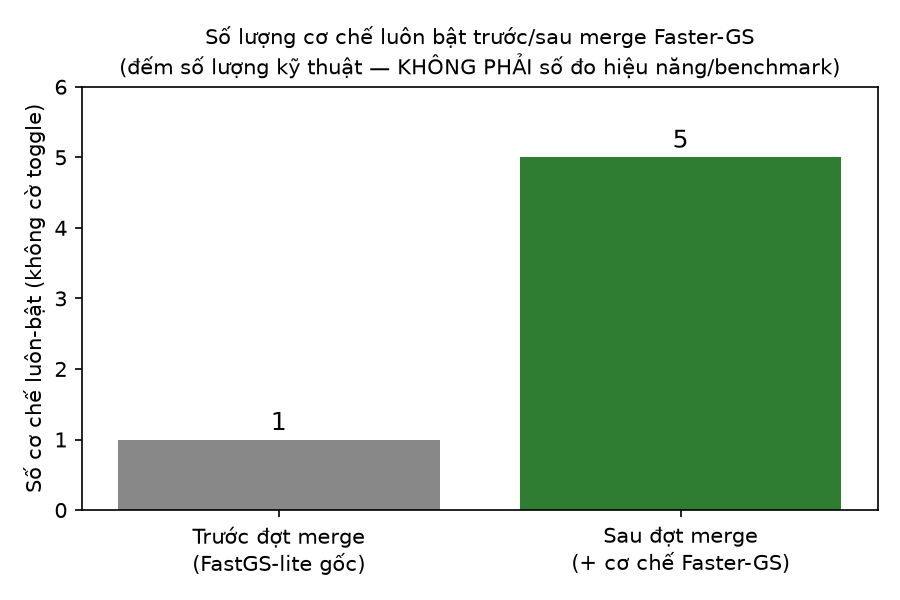
\includegraphics[width=0.3\linewidth]{../BOOK/fastergs_merge_figures/00_techniques_overview.png}
\captionof{figure}{\footnotesize Sơ đồ khối: đường đi dữ liệu từ structure tensor ảnh $\to$ eta 3 kênh $\to$ quyết định split/clone/prune}
\end{frame}

% --- Slide 2: Vì sao cần Structure-Aware? ---
\begin{frame}{Vì sao cần "Structure-Aware"? Trực giác Nyquist}
\begin{columns}[T]
\begin{column}{0.52\linewidth}
\footnotesize
\begin{itemize}
    \item \textbf{3DGS gốc}: tín hiệu densify duy nhất là \emph{screen-space positional gradient} trung bình -- Gaussian nào có gradient vị trí lớn (đóng góp nhiều vào việc giảm loss) thì được clone/split, bất kể kích thước hình học thực tế so với chi tiết ảnh. Rasterizer nền cũng giới hạn vùng ảnh hưởng bằng \emph{compact box} ($3\sigma$, hệ số \texttt{mult}$=0.7$) và một \emph{cost model} để tăng tốc, nhưng phần đó không đổi bản chất tín hiệu densify.
    \item \textbf{SADGS}: bỏ hẳn gradient làm tín hiệu chính, thay bằng \textbf{so khớp trực tiếp} kích thước Gaussian với tần số không gian thực đo được trên ảnh.
    \item Trực giác Nyquist: nếu trục Gaussian trên màn hình \textbf{lớn hơn} bước sóng cục bộ của texture $\Rightarrow$ dưới-lấy-mẫu (undersampling) $\Rightarrow$ mờ/alias chi tiết; nếu \textbf{nhỏ hơn nhiều} $\Rightarrow$ lãng phí bộ nhớ và compute mà không tăng chất lượng.
\end{itemize}
\end{column}
\begin{column}{0.46\linewidth}
\centering
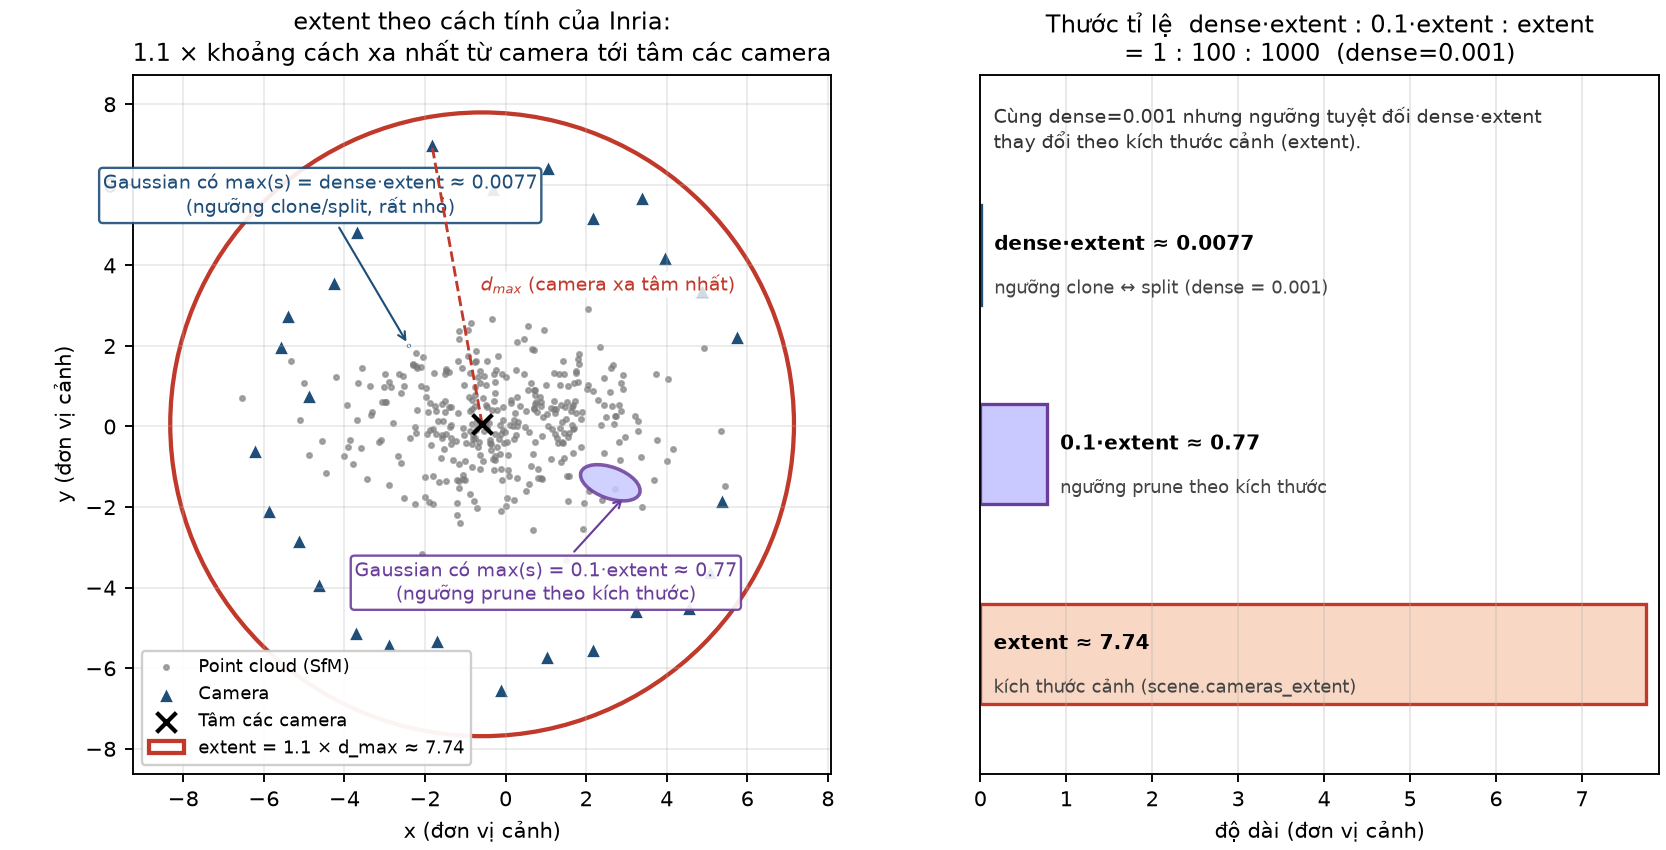
\includegraphics[width=\linewidth]{../BOOK/adc_3dgs/figures/fig_06_scene_extent.png}
\captionof{figure}{\footnotesize Phạm vi cảnh (scene extent) làm cơ sở chuẩn hoá ngưỡng kích thước Gaussian -- điểm khác biệt so với gradient thuần tuý của 3DGS gốc.}
\end{column}
\end{columns}
\end{frame}

% --- Slide 3: Dòng thời gian nghiên cứu + bảng so sánh 2 cột ---
\begin{frame}{Dòng thời gian: 3DGS $\to$ SADGS}
\footnotesize
\begin{itemize}
    \item \textbf{3DGS} (Kerbl et al., SIGGRAPH 2023): đặt nền móng densify/prune dựa trên gradient vị trí tích luỹ, split đẳng hướng bằng lấy mẫu ngẫu nhiên $\mathcal{N}(0, \mathrm{diag}(s^2))$.
    \item \textbf{SADGS} (Lyu et al., SIGGRAPH 2026 -- MPI Informatik, Cambridge, VIA): thay tín hiệu bằng tần số cấu trúc đa tỉ lệ $\eta$, split \textbf{dị hướng theo từng trục}, tích luỹ qua \textbf{nhiều view} trước khi quyết định.
\end{itemize}
\begin{table}
\centering
\begin{tabular}{lcc}
\toprule
\textbf{Tiêu chí} & \textbf{3DGS gốc} & \textbf{SADGS} \\
\midrule
Tín hiệu densify & grad vị trí & tần số $\eta$ đa tỉ lệ \\
Split dị hướng theo trục & không & có ($k_\text{axis}=\lceil\sqrt{\eta_\text{axis}}\rceil$) \\
Số view dùng để quyết định & 1 (tức thời) & nhiều (multiview-consistency) \\
Lưới con khi split & ngẫu nhiên $\mathcal{N}(0,\mathrm{diag}(s^2))$ & lưới tất định theo trục \\
\bottomrule
\end{tabular}
\end{table}
\begin{itemize}
    \item[$\Rightarrow$] Sự khác biệt cốt lõi: SADGS chuyển từ "Gaussian nào đang gây loss lớn" (gradient, tức thời) sang "Gaussian nào có kích thước sai so với tần số ảnh thật, nhất quán qua nhiều góc nhìn" (structure-aware, tích luỹ).
\end{itemize}
\end{frame}

% --- Slide 4: Giới thiệu khái niệm eta bằng ví dụ trực giác ---
\begin{frame}{Khái niệm $\eta$: tỉ số kích thước Gaussian / bước sóng texture}
\begin{columns}[T]
\begin{column}{0.5\linewidth}
\footnotesize
\begin{itemize}
    \item Định nghĩa trực giác: $\eta = \dfrac{\text{độ dài trục Gaussian chiếu màn hình}}{\text{bước sóng cục bộ của texture}}$.
    \item Ví dụ đơn giản: một Gaussian có trục chiếu dài 8 pixel, phủ lên vùng có vân texture lặp lại mỗi 4 pixel (bước sóng $=4$) $\Rightarrow \eta = 8/4 = 2$.
    \item $\eta \approx 1$: kích thước Gaussian \textbf{vừa khớp} bước sóng -- điểm cân bằng Nyquist, không cần densify/prune thêm.
    \item $\eta > 1$ (ví dụ trên, $\eta=2$): Gaussian \textbf{quá to} so với chi tiết $\Rightarrow$ cần \textbf{split} để giảm kích thước, tăng độ phân giải cục bộ.
    \item $\eta < 1$ (ví dụ: trục 2 pixel trên vùng bước sóng 4 pixel $\Rightarrow \eta=0.5$): Gaussian \textbf{quá nhỏ} $\Rightarrow$ ứng viên cho \texttt{expand\_undersized\_gs} (giãn) hoặc giữ nguyên nếu vùng đã đủ mượt.
    \item Ngưỡng cứng dùng trong phân loại: \texttt{TAU\_HIGH}$=1.0$ (trên $\eta$ này coi là "high", cần split), \texttt{TAU\_LOW}$=0.1$ (dưới ngưỡng này coi là "low"). Công thức đầy đủ (2 chế độ \texttt{wavelength}/\texttt{projection}) sẽ trình bày ở phần tiếp theo.
\end{itemize}
\end{column}
\begin{column}{0.48\linewidth}
\centering
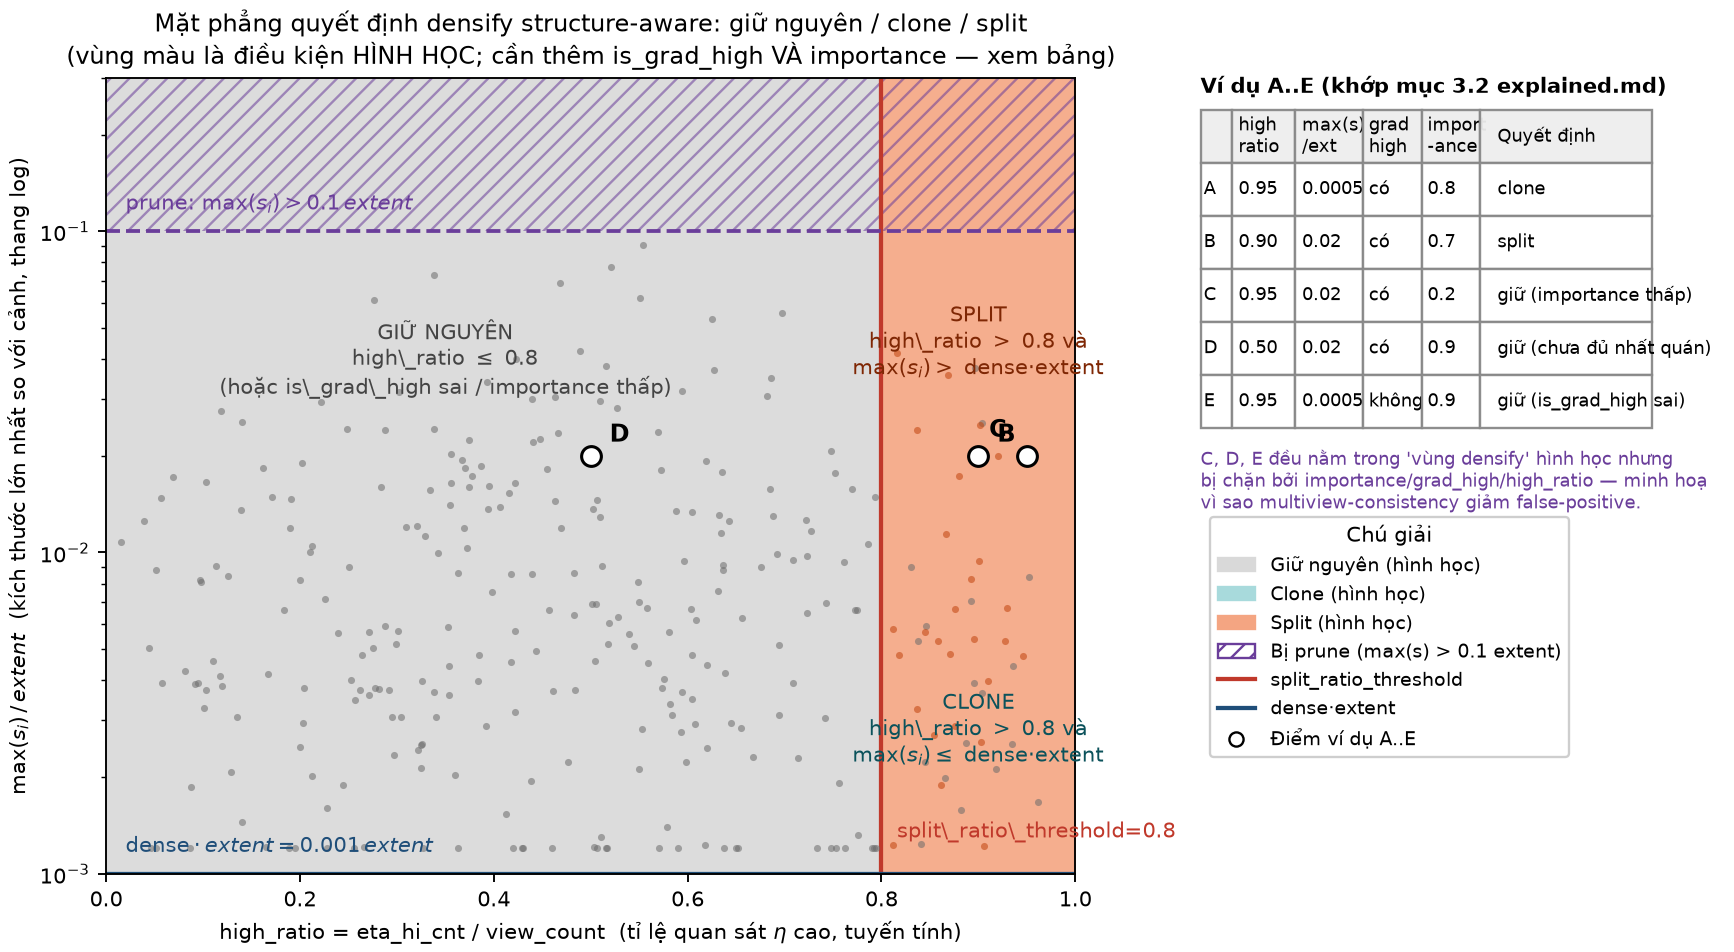
\includegraphics[width=\linewidth]{../BOOK/adc_3dgs/figures/fig_05_decision_plane.png}
\captionof{figure}{\footnotesize Mặt phẳng quyết định theo $\eta$: vùng split ($\eta$ cao), vùng ổn định ($\eta \approx 1$), vùng giãn/expand ($\eta$ thấp).}
\end{column}
\end{columns}
\end{frame}

% --- Slide 5: Lộ trình 8 phần tiếp theo ---
\begin{frame}{Lộ trình: 8 phần trình bày cơ chế SADGS}
\footnotesize
\begin{itemize}
    \item \textbf{Phần 2 -- Đo tần số}: \texttt{update\_freq\_stats\_online} tính structure tensor đa tỉ lệ, hai chế độ \texttt{eta\_compute\_mode} (\texttt{wavelength} dựa trị riêng $\lambda_1$, \texttt{projection} chiếu dạng toàn phương lên từng trục).
    \item \textbf{Phần 3 -- Clone}: \texttt{densify\_and\_clone\_structgs}, điều kiện dựa trên \texttt{importance\_score} (accum view count) so với ngưỡng $0.5$.
    \item \textbf{Phần 4 -- Split dị hướng}: \texttt{densify\_and\_split\_structgs}, lưới con tất định theo từng trục $k_\text{axis}=\lceil\sqrt{\eta_\text{axis}}\rceil$, khác 3DGS gốc lấy mẫu ngẫu nhiên.
    \item \textbf{Phần 5 -- Giãn Gaussian dưới cỡ}: \texttt{expand\_undersized\_gs}, bước giải tích $\Delta\log(\text{scale}) = -0.5\log(\eta)$ để đưa $\eta \to 1$ \alert{(hiện không được gọi trong \texttt{train.py})}.
    \item \textbf{Phần 6 -- Densify + prune 1 vòng}: \texttt{densify\_and\_prune\_structgs}, kết hợp \texttt{high\_ratio}/\texttt{split\_ratio\_threshold} $=0.8$ và \texttt{densify\_grad\_threshold}.
    \item \textbf{Phần 7 -- Prune cuối multi-view}: \texttt{final\_prune\_structgs}, loại bỏ khi \texttt{opacity}$<$\texttt{min\_opacity} hoặc \texttt{pruning\_score}$>0.9$ \alert{(hiện không được gọi trong \texttt{train.py})}.
    \item \textbf{Phần 8 -- Tổng kết}: so sánh hiệu quả, các tham số dead-code, và giới hạn thực nghiệm của SADGS so với 3DGS gốc.
\end{itemize}
\end{frame}

% ============================================================
% PHẦN SADGS — Slide 2/8: Structure Tensor & tỉ số tần số eta
% ============================================================

% --- Frame 1 ---
\begin{frame}{Đo cấu trúc texture đa tỉ lệ: Structure Tensor $\to$ $\eta$}
\footnotesize
\begin{itemize}
    \item Với mỗi camera nhìn thấy Gaussian, lấy mẫu \textbf{structure tensor} $S$ tại điểm chiếu $(u,v)$ trên ảnh gốc (được tiền tính đa tỉ lệ, \texttt{st\_levels} mức, \texttt{st\_mode}):
\end{itemize}
\[
S = \begin{pmatrix} S_{xx} & S_{xy} \\ S_{xy} & S_{yy}\end{pmatrix}, \qquad
\lambda_1 = \frac{\text{tr}(S)}{2} + \sqrt{\left(\frac{\text{tr}(S)}{2}\right)^2 - \det(S)}
\]
\begin{itemize}
    \item $\lambda_1$ là trị riêng lớn nhất (năng lượng gradient cực đại) $\Rightarrow$ \textbf{bước sóng cục bộ} $w_{\min} = 1/(\sqrt{\lambda_1}+\varepsilon)$ (đơn vị pixel) -- vùng chi tiết mịn có $w_{\min}$ nhỏ, vùng phẳng có $w_{\min}$ lớn.
    \item Chiều dài trục chiếu 2D của Gaussian (từ Jacobian phối cảnh $J$, ma trận xoay $R$, scale $\Sigma$): $\text{axis}_k = \lVert J R \,\text{diag}(\Sigma)\, e_k\rVert$, $k\in\{x,y,z\}$.
\end{itemize}
\[
\eta_k^{\text{wavelength}} = \frac{\text{axis}_k}{w_{\min}}, \qquad
\eta_k^{\text{projection}} = \sqrt{\,e_k^\top R^\top J^\top S J R\, e_k\,}
\]
\begin{itemize}
    \item Hai chế độ (\texttt{eta\_compute\_mode}): \texttt{"wavelength"} (mặc định, so kích thước Gaussian với bước sóng texture) hoặc \texttt{"projection"} (chiếu trực tiếp structure tensor lên từng trục).
    \item $\eta_k > 1$: trục $k$ của Gaussian \textbf{lớn hơn} chi tiết ảnh tại đó $\Rightarrow$ nguy cơ alias/mờ $\Rightarrow$ ứng viên split theo trục đó.
    \item $\eta$ được tính \textbf{riêng cho từng trục} ($\eta_{3ch}$, 3 kênh), không phải một số vô hướng chung cho cả Gaussian.
\end{itemize}
\end{frame}

% --- Frame 2 ---
\begin{frame}{Structure tensor đa tỉ lệ là gì?}
\begin{columns}
\begin{column}{0.55\textwidth}
\footnotesize
\begin{itemize}
    \item $S$ được xây từ \textbf{DoG (Difference of Gaussians)} đa octave trên ảnh ground-truth (\texttt{loss\_utils.py: get\_multiscale\_structure\_tensor\_v1}): structure tensor gốc $S_{\text{base}}$ (Di Zenzo + Sobel) được tích phân lại ở mỗi octave với $\rho_i = 3\sigma_i$ thành $S_i$, chuẩn hoá hướng $\hat S_i = S_i/(\mathrm{tr}\,S_i+\varepsilon)$ rồi cộng dồn có trọng số
    $S = \frac{1}{\sum_i w_i+\varepsilon}\sum_i \hat S_i\, w_i\, f_i^2$, với $w_i = \lVert I_{\sigma_i}-I_{\sigma_{i+1}}\rVert_2^{\,p}$ ($p=$\texttt{power\_factor}$=3$) và $f_i = 1/\texttt{octave\_step}^i$.
    \item Kết quả được \textbf{cache theo ảnh} và tra cứu lại trong \texttt{update\_freq\_stats\_online}, không tính lại mỗi iteration -- giữ chi phí runtime thấp.
    \item Trị riêng lớn nhất $\lambda_1$ của $S$ = hướng \& độ mạnh của biến thiên cường độ pixel mạnh nhất tại điểm đó $\Rightarrow$ chính là \textbf{tần số không gian cục bộ} cao nhất của texture.
    \item Vùng cạnh sắc/hoạ tiết dày đặc $\Rightarrow$ $\lambda_1$ lớn $\Rightarrow$ $w_{\min}$ nhỏ $\Rightarrow$ đòi hỏi Gaussian nhỏ để không làm mờ chi tiết.
    \item Vùng mảng màu phẳng (tường, bầu trời) $\Rightarrow$ $\lambda_1$ nhỏ $\Rightarrow$ $w_{\min}$ lớn $\Rightarrow$ Gaussian lớn vẫn đủ, không cần chi tiết thêm.
\end{itemize}
\end{column}
\begin{column}{0.45\textwidth}
\centering
\includegraphics[width=0.95\linewidth]{fig_07_threshold_sweep.png}
\captionof{figure}{\footnotesize Minh hoạ định tính: độ nhạy của phân loại tần số khi quét ngưỡng $\tau$}
\end{column}
\end{columns}
\end{frame}

% --- Frame 3 ---
\begin{frame}{Phân loại quan sát: high / mid / low}
\footnotesize
\begin{itemize}
    \item Mỗi \textbf{quan sát} (một Gaussian trong một view) được gán nhãn dựa trên $\eta_{\max}=\max_k \eta_k$ lấy trên 3 trục (\texttt{freq\_utils.py:401}), theo hai ngưỡng cứng:
\end{itemize}
\[
\text{label}(\eta_{\max}) =
\begin{cases}
\text{\textbf{high}} & \eta_{\max} > \tau_{\text{high}} = 1.0 \quad \text{(chi tiết vượt kích thước hiện tại} \Rightarrow \text{ứng viên split)} \\
\text{\textbf{low}} & \eta_{\max} \le \tau_{\text{low}} = 0.1 \quad \text{(Gaussian thừa chi tiết so với texture} \Rightarrow \text{ứng viên prune)} \\
\text{mid} & \tau_{\text{low}} < \eta_{\max} \le \tau_{\text{high}} \quad \text{(giữ nguyên)}
\end{cases}
\]
\vspace{0.15cm}
\centering
\begin{tabular}{lccccl}
\toprule
\textbf{Ví dụ} & $\eta_x$ & $\eta_y$ & $\eta_z$ & $\eta_{\max}$ & \textbf{Nhãn của quan sát} \\
\midrule
Gaussian A & 1.3 & 0.4 & 0.08 & 1.3 & \textbf{high} $\Rightarrow$ \texttt{eta\_high\_count} $+1$ \\
Gaussian B & 0.6 & 0.5 & 0.7 & 0.7 & mid $\Rightarrow$ \texttt{eta\_mid\_count} $+1$ \\
Gaussian C & 0.08 & 0.05 & 0.03 & 0.08 & \textbf{low} $\Rightarrow$ \texttt{eta\_low\_count} $+1$ \\
\bottomrule
\end{tabular}
\vspace{0.2cm}
\begin{itemize}
    \item Nhãn high/mid/low chỉ quyết định \textbf{có} split/prune hay không. \textbf{Mức độ} chia mới dùng $\eta$ \textbf{riêng từng trục}: \texttt{max\_eta\_3ch} (max qua các view, \texttt{freq\_utils.py:390--392}) $\to k_{\text{axis}}$ ở Slide~4.
    \item Ngưỡng lọc bổ sung \texttt{freq\_grad\_threshold} và \texttt{importance\_score\_threshold} ($=0.5$) giúp loại các tín hiệu tần số yếu/nhiễu trước khi đưa vào quyết định densify.
\end{itemize}
\end{frame}

% --- Frame 4 ---
\begin{frame}{Tính nhất quán đa góc nhìn (multiview-consistency)}
\begin{columns}
\begin{column}{0.55\textwidth}
\footnotesize
\begin{itemize}
    \item Một Gaussian được nhiều camera nhìn thấy trong quá trình huấn luyện; mỗi view cho một ước lượng $\eta_k$ khác nhau (do góc chiếu, occlusion, độ phân giải khác nhau).
    \item \texttt{update\_freq\_stats\_online} \textbf{tích luỹ} qua từng view vào bộ đếm trên mỗi Gaussian: \texttt{accum\_eta}, \texttt{eta\_high\_count}, \texttt{eta\_low\_count}, \texttt{accum\_view\_count}.
\end{itemize}
\[
\text{high\_ratio} = \frac{\texttt{eta\_high\_count}}{\texttt{accum\_view\_count}}, \qquad
\text{low\_ratio} = \frac{\texttt{eta\_low\_count}}{\texttt{accum\_view\_count}}
\]
\begin{itemize}
    \item Chỉ khi \text{high\_ratio} (hoặc \text{low\_ratio}) đủ lớn qua \textbf{nhiều view} thì Gaussian mới thực sự được coi là cần split (hoặc prune).
    \item Lý do: một view đơn lẻ có thể bị occlusion, mờ do chuyển động, hoặc góc nhìn xấu $\Rightarrow$ tín hiệu $\eta$ nhiễu tại view đó. Tích luỹ đa view giúp lọc nhiễu, tránh split/prune sai vì một khung hình bất thường.
\end{itemize}
\end{column}
\begin{column}{0.45\textwidth}
\centering
\includegraphics[width=0.95\linewidth]{fig_04_gbar_history.png}
\captionof{figure}{\footnotesize Minh hoạ khái niệm: giá trị tích luỹ ổn định dần qua nhiều lần cập nhật (hình gốc vẽ cho gradient trung bình, dùng ở đây để minh hoạ ý tưởng tích luỹ theo view, không phải đúng 100\% cơ chế $\eta$)}
\end{column}
\end{columns}
\end{frame}

% --- Frame 5 ---
\begin{frame}{So sánh hai chế độ \texttt{eta\_compute\_mode}}
\footnotesize
\centering
\begin{tabular}{lll}
\toprule
\textbf{Tiêu chí} & \textbf{"wavelength"} & \textbf{"projection"} \\
\midrule
Công thức & $\eta_k = \text{axis}_k / w_{\min}$ & $\eta_k = \sqrt{e_k^\top R^\top J^\top S J R\, e_k}$ \\
Ý nghĩa & So kích thước Gaussian & Chiếu trực tiếp dạng toàn phương \\
 & với 1 con số bước sóng vô hướng & của $S$ lên từng trục Gaussian \\
Thông tin dùng từ $S$ & Chỉ $\lambda_1$ (trị riêng lớn nhất) & Toàn bộ ma trận $S$ (cả hướng) \\
Độ nhạy hướng & Đẳng hướng (isotropic) theo $w_{\min}$ & Bất đẳng hướng, theo đúng hướng trục \\
Vai trò & Chế độ mặc định, đơn giản, ổn định & Lựa chọn thiết kế thay thế, tận dụng \\
 & & đầy đủ thông tin hướng của $S$ \\
\bottomrule
\end{tabular}
\vspace{0.3cm}
\begin{itemize}
    \item \textbf{"wavelength"}: quy $S$ về một đại lượng vô hướng ($\lambda_1 \to w_{\min}$) rồi so trực tiếp với độ dài trục -- đơn giản, dễ diễn giải như "kích thước Gaussian so với chi tiết ảnh".
    \item \textbf{"projection"}: giữ nguyên thông tin hướng của $S$, chiếu quadratic form lên từng trục $e_k$ -- có thể phân biệt tốt hơn khi texture có tính bất đẳng hướng mạnh (vd. vân gỗ, sọc kẻ).
    \item Đây là hai lựa chọn thiết kế đã cài sẵn trong \texttt{arguments/\_\_init\_\_.py} (\texttt{eta\_compute\_mode}); code không kèm ghi chú lý do chọn mặc định, nên không suy diễn thêm ngoài khác biệt công thức nêu trên.
\end{itemize}
\end{frame}

% ============================================================
% PHẦN SADGS — Slide 3/8: Clone dựa trên importance đa view (densify_and_clone_structgs)
% ============================================================

\begin{frame}{Nhân bản Gaussian nhỏ nhưng quan trọng (\texttt{densify\_and\_clone\_structgs})}
\footnotesize
\begin{itemize}
    \item Clone dùng cho Gaussian \textbf{còn nhỏ} (chưa cần chia hình học) nhưng đang thiếu mật độ tại vùng có chi tiết -- nhân đôi giữ nguyên scale/rotation/màu, chỉ khác vị trí do phép cộng tensor.
    \item \textbf{3DGS gốc}: điều kiện clone dựa trên \textit{gradient vị trí trung bình} $\lVert\bar g_{xyz}\rVert \ge \tau_{\text{grad}}$ tích luỹ qua backprop -- tín hiệu gián tiếp, nhiễu theo batch view ngẫu nhiên mỗi bước.
    \item \textbf{SADGS}: thay/bổ sung bằng tín hiệu \textbf{tần số -- importance đa view} $\Rightarrow$ Gaussian chỉ được clone khi nhiều góc nhìn khác nhau \textit{đồng thuận} rằng nó cần thêm mật độ, không chỉ 1 view nhiễu tức thời.
\end{itemize}
\vspace{0.2cm}
\small
\centering
\begin{tabular}{lll}
\toprule
\textbf{Tiêu chí} & \textbf{3DGS gốc} & \textbf{SADGS} \\
\midrule
Tín hiệu chọn & Gradient vị trí $\bar g_{xyz}$ & Importance đa view (\texttt{accum\_view\_count}) \\
Điều kiện scale & $\max(\sigma) \le$ \texttt{percent\_dense}$\times$extent & $\max(\sigma) \le$ \texttt{dense}$\times$extent \\
Hàm nhân bản & \texttt{densify\_and\_clone} & \texttt{densify\_and\_clone\_structgs} \\
\bottomrule
\end{tabular}
\end{frame}

% --- Frame 2 ---
\begin{frame}{Điều kiện clone chi tiết}
\footnotesize
Trong \texttt{densify\_and\_prune\_structgs}, một Gaussian được đưa vào tập ứng viên clone khi thoả \textbf{đồng thời} hai lớp điều kiện:
\[
\texttt{clone\_qualifiers} = \big(\max_{\text{axis}}(\sigma) \le \texttt{dense}\times\text{extent}\big), \qquad \texttt{dense}=0.001
\]
\[
\texttt{final\_clone\_mask} = \big(\texttt{grad\_qualifiers} \lor \texttt{full\_split\_mask}\big) \wedge \texttt{clone\_qualifiers}
\]
\begin{itemize}
    \item $\texttt{grad\_qualifiers} = \lVert\bar g_{xyz}\rVert \ge \texttt{grad\_thresh}\,(0.0002)$ -- vẫn giữ tín hiệu gradient chuẩn làm điều kiện cần.
    \item Nhưng để \textbf{thực sự} được nhân bản, còn phải vượt qua bộ lọc \textbf{importance} tính trên toàn cục:
\end{itemize}
\[
\texttt{importance\_score} = \texttt{accum\_view\_count}, \qquad
\texttt{metric\_mask} = \big(\texttt{importance\_score} > \texttt{importance\_score\_threshold}\big),\ \tau{=}0.5
\]
\begin{itemize}
    \item \texttt{accum\_view\_count}: số lần Gaussian được tích luỹ thống kê tần số $\eta$ qua các view liên tiếp -- Gaussian hiếm khi "được nhìn thấy và cần" (đóng góp tần số cao) sẽ có điểm thấp, bị loại dù gradient tức thời cao.
    \item Lệnh gọi thực thi: \texttt{densify\_and\_clone\_structgs(metric\_mask, final\_clone\_mask)} -- bên trong lấy \texttt{selected = metric\_mask \(\wedge\) final\_clone\_mask} rồi copy nguyên các tensor tại các chỉ số đó.
\end{itemize}
\end{frame}

% --- Frame 3 ---
\begin{frame}{Ví dụ số: Gaussian nào được clone?}
\footnotesize
Giả sử extent$=6.0$ $\Rightarrow$ ngưỡng scale $= \texttt{dense}\times\text{extent} = 0.001\times 6.0 = 0.006$; ngưỡng gradient $\texttt{grad\_thresh}=0.0002$; ngưỡng importance $\tau=0.5$ (giả định thang $[0,1]$ đã chuẩn hoá theo số view tối đa quan sát được).
\vspace{0.15cm}
\centering
\begin{tabular}{lccccc}
\toprule
\textbf{GS} & $\max(\sigma)$ & $\lVert\bar g_{xyz}\rVert$ & importance & scale đạt? & \textbf{Kết luận} \\
\midrule
$A$ & $0.004$ & $0.00035$ & $0.72$ & \checkmark & \textbf{Clone} (nhỏ, gradient cao, đa view đồng thuận) \\
$B$ & $0.004$ & $0.00031$ & $0.30$ & \checkmark & Không clone (importance dưới $0.5$ -- chỉ 1--2 view nhiễu) \\
$C$ & $0.009$ & $0.00040$ & $0.85$ & $\times$ & Không clone -- chuyển sang \textbf{split} (đã đủ lớn, xem Slide~4) \\
\bottomrule
\end{tabular}
\vspace{0.2cm}
\begin{itemize}
    \item $A$: thoả cả 3 điều kiện $\Rightarrow$ nhân bản thành 2 Gaussian trùng vị trí, sau đó optimizer sẽ tách chúng dần qua các bước gradient tiếp theo.
    \item $B$: gradient tức thời cao nhưng importance thấp $\Rightarrow$ SADGS coi đây là nhiễu 1 view, \textbf{không} lãng phí ngân sách điểm.
    \item $C$: điều kiện scale không thoả ($\max(\sigma) > 0.006$) $\Rightarrow$ dù importance cao vẫn không clone, mà rơi vào nhánh split.
\end{itemize}
\end{frame}

% --- Frame 4 ---
\begin{frame}{Trực quan hoá trước/sau clone}
\begin{columns}
\begin{column}{0.5\textwidth}
\centering
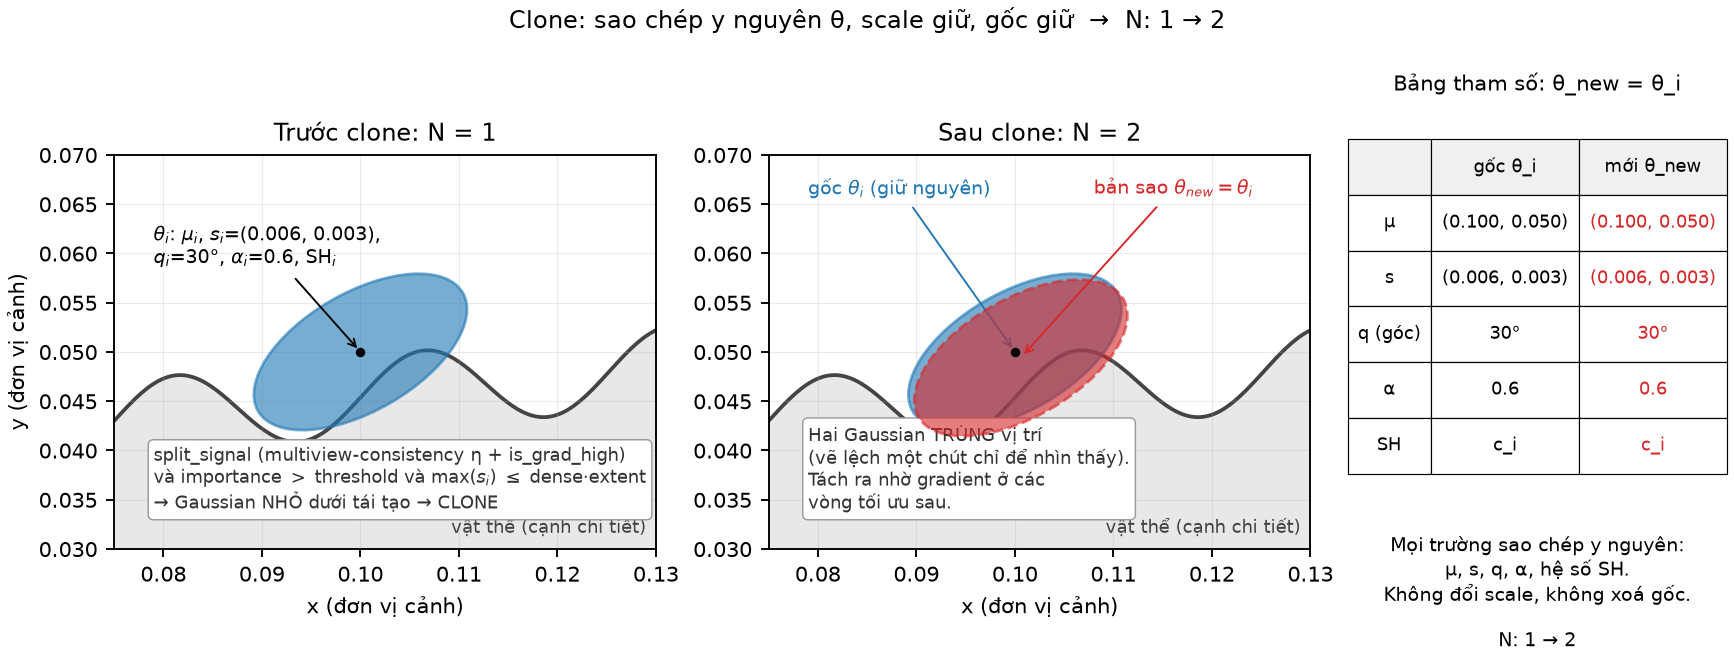
\includegraphics[width=0.95\linewidth]{../BOOK/adc_3dgs/figures/fig_08_clone_before_after.png}
\captionof{figure}{\footnotesize Trước/sau khi clone: Gaussian nhỏ được nhân đôi tại cùng vị trí, giữ nguyên scale/rotation}
\end{column}
\begin{column}{0.5\textwidth}
\footnotesize
\begin{itemize}
    \item Hình minh hoạ \textbf{toy model} tổng quát cơ chế clone (copy nguyên tham số, không đổi hình học) -- \textbf{không} phải render thật từ một cảnh/dataset cụ thể của SADGS.
    \item Sau \texttt{densification\_postfix}: 2 Gaussian con có \textit{cùng} $\mu, \Sigma$, opacity, SH -- chỉ khác nhau ở chỗ chúng là 2 tham số riêng biệt trong optimizer (2 hàng tensor), nên gradient tiếp theo có thể đẩy chúng ra 2 hướng khác nhau.
    \item Bộ đếm \texttt{densify\_count} \textbf{không} tăng khi clone (khác với split) -- vì clone không thay đổi độ mịn hình học, chỉ tăng số lượng điểm phủ vùng đó.
    \item Các bộ tích luỹ tần số (\texttt{accum\_eta}, \texttt{accum\_view\_count}, \texttt{eta\_high/mid/low\_count}) của 2 Gaussian con được khởi tạo lại bằng $0$ -- chúng "bắt đầu lại" quá trình tích luỹ thống kê đa view.
\end{itemize}
\end{column}
\end{columns}
\end{frame}

% --- Frame 5 ---
\begin{frame}{Vì sao clone khác split? Liên hệ sang Slide 4}
\footnotesize
\begin{itemize}
    \item \textbf{Clone}: chỉ \textit{nhân bản} (copy) -- không đổi hình học của từng Gaussian con, không xoay, không co scale. Mục tiêu: tăng \textbf{số lượng điểm} tại vùng mật độ thấp nhưng kích thước Gaussian còn phù hợp với chi tiết ảnh ($\eta$ chưa vượt ngưỡng).
    \item \textbf{Split}: Gaussian đã \textbf{quá lớn} so với chi tiết texture cục bộ ($\max(\sigma) > \texttt{dense}\times\text{extent}$, thường đi kèm $\eta > 1$) $\Rightarrow$ phải \textbf{chia nhỏ hình học} ($\sigma_{\text{new}} = \sigma_{\text{old}}/k$), sinh Gaussian con nhỏ hơn và xoá Gaussian cha.
    \item Cùng dùng chung hàm nội bộ \texttt{densification\_postfix} để nối tensor mới vào optimizer, nhưng khác nhau ở \textbf{có prune Gaussian cha hay không}: clone giữ nguyên cha, split xoá cha (\texttt{prune\_points} sau khi sinh con).
\end{itemize}
\vspace{0.2cm}
\small
\centering
\begin{tabular}{lll}
\toprule
\textbf{Tiêu chí} & \textbf{Clone (Slide 3)} & \textbf{Split (Slide 4)} \\
\midrule
Điều kiện scale & $\max(\sigma)\le\texttt{dense}\times\text{extent}$ & $\max(\sigma) > \texttt{dense}\times\text{extent}$ \\
Hình học con & Giống hệt cha & Chia nhỏ theo $k=\lceil\sqrt{\eta}\rceil$/trục \\
Gaussian cha & Giữ lại & Bị prune (xoá) \\
\texttt{densify\_count} & Không đổi & Tăng $+1$ (kế thừa cha) \\
\bottomrule
\end{tabular}
\end{frame}

% ============================================================
% PHẦN SADGS — Slide 4/8: Giãn Gaussian dưới cỡ (expand_undersized_gs)
% ============================================================

\begin{frame}{Vì sao cần "giãn ngược" -- Gaussian quá nhỏ cũng lãng phí ngân sách \alert{(cơ chế này KHÔNG chạy mặc định, xem Slide 4.5)}}
\footnotesize
\begin{itemize}
    \item \alert{Lưu ý ngay từ đầu:} \texttt{expand\_undersized\_gs} được \textbf{định nghĩa đầy đủ} trong \texttt{gaussian\_model.py}, nhưng lời gọi duy nhất tới nó trong \texttt{train.py:356--359} \textbf{đang bị comment out} -- mặc định SADGS \textbf{không} chạy bước "giãn ngược" mô tả dưới đây, chỉ clone/split. Chi tiết ở frame cuối và ở \texttt{part\_sadgsx\_06}.
    \item ADC gốc (3DGS) chỉ có 2 phản ứng khi Gaussian sai cỡ: \textbf{clone} (nhân bản, cho vùng thiếu điểm) và \textbf{split} (chia nhỏ, cho vùng thừa điểm) -- không có cơ chế \textbf{thu gọn số lượng} khi một vùng đã bị chia \emph{quá mức cần thiết}.
    \item SADGS đo $\eta = \text{axis}_k / w_{\min}$ (\texttt{freq\_utils.py:348}): tỉ số giữa độ dài trục chiếu màn hình của Gaussian và bước sóng cục bộ của texture -- đã dùng để \textbf{chia} khi $\eta$ quá lớn (Slide 3). \alert{Lưu ý:} docstring của \texttt{expand\_undersized\_gs} (\texttt{gaussian\_model.py:838}) lại giả định $\eta=(\sigma\omega)^2$ -- một mâu thuẫn với $\eta$ tuyến tính thực sự được tính (hệ quả ở slide sau).
    \item Chiều ngược lại: nếu $\eta$ \textbf{quá nhỏ} ($0 < \eta < \tau_{\text{expand}}$, tham số \texttt{tau\_expand}, mặc định $1.0$), Gaussian đang \emph{mờ hơn mức cần thiết} so với chi tiết cục bộ -- một Gaussian to hơn có thể phủ đúng vùng đó mà \textbf{không mất chi tiết} và không tốn thêm 1 điểm nào trong ngân sách.
    \item Đây là đòn bẩy thứ ba của SADGS bên cạnh clone/split: \textbf{sửa scale tại chỗ bằng công thức giải tích}, không cần thêm/xoá Gaussian, không cần lặp gradient descent.
\end{itemize}
\end{frame}

% --- Slide mới: công thức giải tích ---
\begin{frame}{Công thức giải tích: co/giãn đúng \emph{một bước} tới biên Nyquist}
\footnotesize
\begin{itemize}
    \item Mục tiêu đặt ra trong docstring: $\eta_{\text{new}} = 1$. Với \emph{giả định} $\eta\propto\sigma^2$ của docstring (\texttt{gaussian\_model.py:837--840}):
\end{itemize}
\[
\eta_{\text{new}} = \Big(\frac{\sigma_{\text{target}}}{\sigma_{\text{old}}}\Big)^2 \eta_{\text{old}} = 1
\;\Longrightarrow\;
\sigma_{\text{target}} = \frac{\sigma_{\text{old}}}{\sqrt{\eta_{\text{old}}}}
\]
\begin{itemize}
    \item Vì scale được lưu trong \textbf{log-space} (\texttt{self.\_scaling}, qua \texttt{scaling\_inverse\_activation}), phép chia trên trở thành một \textbf{phép cộng trực tiếp}:
\end{itemize}
\[
\log\sigma_{\text{target}} = \log\sigma_{\text{old}} - \tfrac12\log\eta_{\text{old}}
\quad\Longleftrightarrow\quad
\Delta\!\log\sigma = -\tfrac12\log\eta
\]
\begin{itemize}
    \item Code (\texttt{expand\_undersized\_gs}, \texttt{gaussian\_model.py:833--864}): \texttt{eta\_vals = clamp(eta, min=1e-6)} (tránh $\log 0$), rồi \texttt{delta\_log\_scale = -0.5*torch.log(eta\_vals)} cộng thẳng vào \texttt{self.\_scaling} -- \textbf{không lặp, không tối ưu}, 1 phép gán tensor là xong.
    \item \alert{Nhưng} $\eta$ thực tế \textbf{tuyến tính} theo $\sigma$ ($\eta=\text{axis}/w_{\min}$), nên $\sigma\!\to\!\sigma/\sqrt{\eta}$ chỉ cho $\eta_{\text{new}}=\sqrt{\eta}$ --- \emph{rút căn} khoảng cách tới $1$, không đạt $1$ như comment \texttt{":853"} tuyên bố. Muốn đúng một bước phải dùng $\Delta\!\log\sigma=-\log\eta$.
\end{itemize}
\end{frame}

% --- Slide mới: dị hướng theo trục + so sánh với split ---
\begin{frame}{Cũng dị hướng theo từng trục -- nhưng ngược chiều với split}
\footnotesize
\begin{itemize}
    \item Giống split (Slide 3), \texttt{expand\_undersized\_gs} nhận \texttt{max\_eta\_3ch} -- $\eta$ tách riêng theo 3 trục $x,y,z$ -- và chỉ sửa trục nào thoả điều kiện:
\end{itemize}
\[
\text{undersized\_mask}_{\text{axis}} = \big(0 < \eta_{\text{axis}} < \tau_{\text{expand}}\big)
\]
\begin{itemize}
    \item Trục không thoả điều kiện (đã đúng cỡ hoặc đang quá lớn, chờ split) được \textbf{giữ nguyên} -- \texttt{delta} chỉ khác 0 tại các trục dưới cỡ, nên một Gaussian có thể vừa "đủ cỡ" theo trục này vừa "được giãn" theo trục khác trong cùng 1 bước.
    \item Khác biệt cốt lõi với split: split dùng $k=\lceil\sqrt{\eta}\rceil$ (làm tròn lên số nguyên $\ge 1$) để nhân bản thành lưới $k_x\times k_y\times k_z$ Gaussian con; expand dùng $\sqrt{\eta}$ \textbf{liên tục} (không làm tròn) để chia scale ngay trên chính Gaussian đó -- \textbf{số lượng Gaussian không đổi}.
\end{itemize}
\centering
\includegraphics[width=0.3\linewidth]{fig_09_split_geometry.png}
\captionof{figure}{\footnotesize Đối chiếu: hình mượn từ cơ chế split dị hướng (Slide 3) -- nơi $\eta$ lớn sinh lưới $k_x\times k_y\times k_z$ Gaussian con; expand xử lý chiều ngược lại ($\eta$ nhỏ) bằng cách co scale tại chỗ, không sinh thêm điểm}
\end{frame}

% --- Slide mới: ví dụ số ---
\begin{frame}{Ví dụ số: một Gaussian dưới cỡ trên 2/3 trục}
\footnotesize
\begin{itemize}
    \item Giả sử $\tau_{\text{expand}}=1.0$ và một Gaussian có $\eta = (\eta_x,\eta_y,\eta_z) = (0.25,\ 0.64,\ 1.5)$:
\end{itemize}
\centering
\begin{tabular}{lccc}
\toprule
\textbf{Trục} & $\eta_{\text{axis}}$ & Dưới cỡ? ($0<\eta<1$) & $\Delta\log\sigma = -\tfrac12\log\eta$ \\
\midrule
$x$ & $0.25$ & Có & $-\tfrac12\log(0.25) \approx +0.693$ \\
$y$ & $0.64$ & Có & $-\tfrac12\log(0.64) \approx +0.223$ \\
$z$ & $1.5$  & Không (chờ split) & $0$ (giữ nguyên) \\
\bottomrule
\end{tabular}
\vspace{0.2cm}
\footnotesize
\begin{itemize}
    \item Kết quả: $\sigma_x$ tăng theo hệ số $1/\sqrt{0.25}=2\times$, $\sigma_y$ tăng $1/\sqrt{0.64}\approx1.25\times$, $\sigma_z$ giữ nguyên -- Gaussian trở nên "phình" đúng theo hướng đang quá mờ so với chi tiết, còn trục $z$ để dành cho vòng split kế tiếp.
    \item Số lượng Gaussian: vẫn là \textbf{1} (so với split cùng $\eta$ thì $k_z=\lceil\sqrt{1.5}\rceil=2$ nếu $\eta_z$ vượt ngưỡng split, sinh thêm điểm) -- minh hoạ đúng vai trò "tiết kiệm ngân sách" của expand.
\end{itemize}
\centering
\includegraphics[width=0.32\linewidth]{fig_11_N_accounting.png}
\captionof{figure}{\footnotesize Kế toán $N$ theo cơ chế split (tham khảo đối chiếu): expand không cộng thêm vào $N$, chỉ cập nhật $\sigma$ tại chỗ}
\end{frame}

% --- Slide mới: bảng so sánh + vị trí trong pipeline ---
\begin{frame}{So sánh expand vs.\ split và vị trí trong vòng lặp ADC}
\footnotesize
\begin{tabular}{lll}
\toprule
\textbf{Tiêu chí} & \texttt{expand\_undersized\_gs} & \texttt{densify\_and\_split\_structgs} \\
\midrule
Điều kiện kích hoạt & $0<\eta_{\text{axis}}<\tau_{\text{expand}}{=}1.0$ & $\eta_{\text{axis}}\ge 1$ (qua $k\ge\sqrt{\eta}$) \\
Số Gaussian & Không đổi (sửa tại chỗ) & Tăng: $N{=}k_x k_y k_z$ mới thay 1 cũ \\
Công thức scale & $\sigma_{\text{old}}/\sqrt{\eta}$ (liên tục $\Rightarrow \eta_{\text{new}}{=}\sqrt{\eta}$) & $\sigma_{\text{old}}/k^{p}$, $k{=}\lceil\sqrt{\eta}\rceil$, $p{=}$\texttt{ks\_scale\_power}${=}1$ \\
Vị trí/hướng & Không đổi & Dịch theo lưới $k$, xoay bởi $R(q)$ \\
Chi phí & $O(1)$, 1 phép cộng log-space & $O(N)$ điểm mới + prune điểm cũ \\
\bottomrule
\end{tabular}
\vspace{0.3cm}
\begin{itemize}
    \item \alert{Thực trạng:} lời gọi \texttt{gaussians.expand\_undersized\_gs(...)} trong \texttt{train.py:356--359} \textbf{đang bị comment out}, nên cơ chế này \textbf{không chạy} trong luồng huấn luyện mặc định. Về thiết kế, nó được đặt \textbf{ngay trước} clone/split trong cùng bước densify.
    \item Vì cả hai cơ chế đều dựa trên cùng một đại lượng $\eta$ 3 kênh, SADGS xử lý \textbf{cả hai đầu} của sai số mật độ (quá thưa lẫn quá thừa) bằng công cụ toán học nhất quán, thay vì chỉ có "chia đôi khi gradient cao" như ADC 3DGS gốc.
\end{itemize}
\end{frame}

% ============================================================
% PHẦN SADGS — Slide 5/8: Split dị hướng theo trục (densify_and_split_structgs)
% ============================================================

\begin{frame}{Quyết định Clone/Split: ngưỡng gradient + tỉ lệ nhất quán đa view}
\footnotesize
\begin{itemize}
    \item Ngoài gradient chuẩn ($\lVert\bar g\rVert\ge$ \texttt{grad\_thresh}, $\lVert\bar g_{\text{abs}}\rVert\ge$ \texttt{grad\_abs\_thresh}) và điều kiện scale (\texttt{dense}$\times$extent để phân biệt clone/split), SADGS thêm điều kiện \textbf{nhất quán đa góc nhìn} dựa trên bộ đếm $\eta$ tích luỹ ở Slide 2:
\end{itemize}
\[
\text{high\_ratio}_i = \frac{\texttt{eta\_high\_count}_i}{\texttt{accum\_view\_count}_i},\qquad
\text{low\_ratio}_i = \frac{\texttt{eta\_low\_count}_i}{\texttt{accum\_view\_count}_i}
\]
\[
\text{split\_mask} = (\text{high\_ratio} > \texttt{split\_ratio\_threshold}) \,\wedge\, \text{is\_grad\_high}
\]
\begin{itemize}
    \item Nghĩa là: Gaussian chỉ bị đánh dấu split khi nó \textbf{thường xuyên} ($> $\texttt{split\_ratio\_threshold}, mặc định $0.8$) bị đánh giá "quá lớn so với texture" ($\eta > \tau_{\text{high}}{=}1.0$) \textbf{ở nhiều góc nhìn khác nhau}, không chỉ 1 view nhiễu.
    \item Khi \texttt{split\_mask} $=$ true và \texttt{max(scale)} $>$ \texttt{dense}$\times$extent (Gaussian đã đủ lớn về hình học), SADGS gọi \texttt{densify\_and\_split\_structgs(...)} -- cơ chế trọng tâm của slide này.
\end{itemize}
\centering
\includegraphics[width=0.38\linewidth]{fig_10_split_samples.png}
\captionof{figure}{\footnotesize high\_ratio: tỉ lệ view mà Gaussian bị coi là quá lớn so với texture, điều kiện AND nhất quán đa view trước khi split}
\end{frame}

% --- Slide 5b ---
\begin{frame}{Split dị hướng theo từng trục: $k_{\text{axis}} = \lceil\sqrt{\eta_{\text{axis}}}\rceil$}
\footnotesize
\begin{itemize}
    \item Khác với 3DGS gốc (luôn chia 1 Gaussian thành đúng \textbf{2} con, lấy mẫu ngẫu nhiên $\mathcal N(0,\mathrm{diag}(s^2))$), SADGS chia dựa trực tiếp trên mức độ "quá cỡ" $\eta$ của \textbf{từng trục riêng biệt}:
\end{itemize}
\[
k_{\text{axis}} = \left\lceil \sqrt{\eta_{\text{axis}}} \right\rceil, \qquad \eta_{\text{axis}} = \mathrm{clamp}(\eta_{\text{axis}},\ \min{=}1.0)
\]
\[
N_{\text{con}} = k_x \times k_y \times k_z
\]
\begin{itemize}
    \item Code (\texttt{densify\_and\_split\_structgs}, \texttt{scene/gaussian\_model.py} dòng $\sim$638--833): mỗi trục $x,y,z$ được chia \textbf{độc lập} thành $k_{\text{axis}}$ phần trên một \textbf{lưới tất định} (deterministic grid) -- không lấy mẫu ngẫu nhiên như bản gốc.
    \item Đã xác nhận trực tiếp trên code: có \texttt{clamp(min=1)} nhưng \textbf{không có clamp trần (max)} trong công thức $k$, dù tham số \texttt{max\_clones\_per\_axis} (mặc định $8$) có khai báo trong \texttt{arguments/\_\_init\_\_.py} -- đây là 1 trong 6 tham số \textbf{dead code}, không thực sự được dùng để giới hạn $k$ trong hàm này.
\end{itemize}
\end{frame}

% --- Slide 5c ---
\begin{frame}{Vị trí và scale của các Gaussian con}
\footnotesize
\begin{itemize}
    \item \textbf{Lưới con tất định}: $N_{\text{con}}=k_x k_y k_z$ vị trí được đặt đều trên lưới cục bộ, sau đó \textbf{dịch chuyển theo đúng hướng xoay thật} của Gaussian gốc bằng ma trận $R(q_i)$ (quaternion rotation) -- không phải dịch theo trục toạ độ thế giới.
    \item \textbf{Scale mới} của mỗi Gaussian con:
\end{itemize}
\[
\sigma_{\text{new}} = \frac{\sigma_{\text{old}}}{k^{\,\texttt{ks\_scale\_power}}}
\]
\begin{itemize}
    \item \texttt{ks\_scale\_power} (\texttt{arguments/\_\_init\_\_.py} dòng $\sim$138) mặc định $1.0$ -- khác 3DGS gốc vốn chia scale cho hằng số cố định $1.6$ bất kể số con sinh ra.
    \item Sau khi tạo $N_{\text{con}}$ Gaussian con, Gaussian gốc bị \textbf{xoá} (không giữ lại như clone) -- toàn bộ $N_{\text{con}}$ điểm mới được nối vào optimizer qua \texttt{densification\_postfix} (hàm dùng chung với clone).
\end{itemize}
\centering
\includegraphics[width=0.32\linewidth]{fig_09_split_geometry.png}
\captionof{figure}{\footnotesize Lưới con $k_x\times k_y\times k_z$ đặt tất định, dịch theo hướng xoay $R(q_i)$ của Gaussian gốc}
\end{frame}

% --- Slide 5d ---
\begin{frame}{Ví dụ số: split dị hướng chỉ theo trục cần thiết}
\footnotesize
Giả sử một Gaussian có $\eta = (\eta_x,\eta_y,\eta_z) = (4.0,\ 1.0,\ 0.5)$ (trục $x$ quá lớn so với texture, trục $y$ vừa đủ, trục $z$ còn nhỏ):
\vspace{0.15cm}
\centering
\begin{tabular}{lcccc}
\toprule
\textbf{Trục} & $\eta_{\text{axis}}$ & $\mathrm{clamp}(\eta,\min{=}1)$ & $k=\lceil\sqrt{\cdot}\rceil$ & Ghi chú \\
\midrule
$x$ & $4.0$ & $4.0$ & $2$ & Chia đôi theo trục này \\
$y$ & $1.0$ & $1.0$ & $1$ & Không chia (đúng ngưỡng) \\
$z$ & $0.5$ & $1.0$ (clamp) & $1$ & Không chia (chờ expand, Slide 4) \\
\bottomrule
\end{tabular}
\vspace{0.2cm}
\begin{itemize}
    \item $N_{\text{con}} = k_x \cdot k_y \cdot k_z = 2\times1\times1 = 2$ -- \textbf{chỉ} chia theo trục $x$, không lãng phí sinh thêm Gaussian theo các trục đã đúng cỡ (khác 3DGS gốc luôn sinh đúng 2 con bất kể hướng nào gây ra gradient cao).
    \item Nếu $\eta=(4.0,\ 4.0,\ 1.0)$: $k=(2,2,1) \Rightarrow N_{\text{con}}=4$ -- số con tăng đúng theo số trục thực sự cần chi tiết hơn.
\end{itemize}
\end{frame}

% --- Slide 5e ---
\begin{frame}{So sánh: split dị hướng SADGS vs.\ split ngẫu nhiên 3DGS gốc}
\footnotesize
\centering
\begin{tabular}{lll}
\toprule
\textbf{Tiêu chí} & \textbf{3DGS gốc} & \textbf{SADGS (\texttt{\_structgs})} \\
\midrule
Tín hiệu quyết định & Positional gradient $\|\bar g\|$ & $\eta$ (tần số) $+$ multiview-consistency \\
Số con & Luôn $2$ & $N_{\text{con}}=k_x k_y k_z$, thay đổi theo $\eta$ \\
Vị trí con & Lấy mẫu $\mathcal N(0,\mathrm{diag}(s^2))$ & Lưới tất định, dịch theo $R(q_i)$ \\
Scale con & $\sigma_{\text{old}}/1.6$ (hằng số) & $\sigma_{\text{old}}/k^{\texttt{ks\_scale\_power}}$ \\
Dị hướng theo trục? & Không & \textbf{Có} -- từng trục độc lập \\
\bottomrule
\end{tabular}
\vspace{0.3cm}
\begin{itemize}
    \item Điểm mấu chốt: SADGS không còn "đoán" hướng cần chia bằng gradient trung bình (dễ bị nhiễu/mất hướng ở vùng nhiều chi tiết theo 1 trục nhưng phẳng theo 2 trục còn lại) -- mà chia \textbf{đúng theo hướng texture đòi hỏi}, đo trực tiếp từ ảnh gốc.
    \item Liên hệ: split (đây) và expand (Slide 4, \texttt{expand\_undersized\_gs}) xử lý \textbf{hai đầu đối lập} của cùng đại lượng $\eta$ -- split khi $\eta$ quá lớn, expand khi $\eta$ quá nhỏ -- cả hai đều \textbf{dị hướng theo trục}, khác biệt căn bản với ADC 1 chiều của 3DGS gốc.
\end{itemize}
\end{frame}

% ============================================================
% PHẦN SADGS — Slide 6/8: densify_and_prune_structgs — "nhạc trưởng" điều phối
% ============================================================

% --- Frame 1 ---
\begin{frame}{\texttt{densify\_and\_prune\_structgs}: nhạc trưởng điều phối 1 vòng ADC}
\footnotesize
\begin{itemize}
    \item Hàm này được gọi mỗi \texttt{densification\_interval} ($100$ vòng), trong khoảng $[\texttt{densify\_from\_iter}{=}500,\ \texttt{densify\_until\_iter}{=}15000]$. Nó \textbf{không tự tính} tín hiệu -- nó \textbf{nhận vào} các mask/score đã tính sẵn ở \texttt{train.py} rồi \textbf{điều phối} clone/split/prune theo đúng thứ tự:
\end{itemize}
\begin{enumerate}
    \item Tính \texttt{grad\_qualifiers}, \texttt{grad\_qualifiers\_abs} từ gradient tích luỹ chuẩn (kế thừa 3DGS gốc).
    \item Tính \texttt{clone\_qualifiers}/\texttt{split\_qualifiers} theo kích thước: $\max(\text{scale}) \le/> \texttt{args.dense}\times\text{extent}$.
    \item Ghép \texttt{custom\_split\_mask}/\texttt{custom\_prune\_mask} (từ high\_ratio/low\_ratio đa view) vào full mask theo \texttt{viewspace\_points\_indices}.
    \item Kết hợp AND/OR ra \texttt{final\_clone\_mask}, \texttt{final\_split\_mask} $\to$ gọi \texttt{densify\_and\_clone\_structgs} rồi \texttt{densify\_and\_split\_structgs}.
    \item Tính \texttt{prune\_mask} (opacity + kích thước) $\to$ tuỳ chọn multinomial resample $\to$ \texttt{prune\_points}.
    \item Ép trần opacity $\alpha \leftarrow \min(\alpha, 0.8)$ cho toàn bộ Gaussian còn lại.
\end{enumerate}
\begin{itemize}
    \item Toàn bộ 6 bước trên nằm gọn trong \textbf{một lệnh gọi hàm} mỗi 100 vòng -- đây là lý do gọi nó là ``nhạc trưởng'': chính \texttt{train.py} chuẩn bị tín hiệu, còn hàm này thực thi đồng bộ và đúng thứ tự.
\end{itemize}
\end{frame}

% --- Frame 2 ---
\begin{frame}{Hai lớp tín hiệu song song: gradient (cũ) vs.\ tần số/đa view (mới)}
\footnotesize
\begin{itemize}
    \item 3DGS gốc chỉ có \textbf{một} loại tín hiệu densify: chuẩn gradient vị trí trung bình. SADGS giữ nguyên lớp này và \textbf{cộng thêm} một lớp tín hiệu thứ hai dựa trên tần số dao động $\eta$ quan sát qua nhiều view, rồi \textbf{kết hợp} hai lớp bằng AND/OR thay vì thay thế:
\end{itemize}
\vspace{0.2em}
\centering
\begin{tabular}{lll}
\toprule
\textbf{Tiêu chí} & \textbf{Gradient (kế thừa 3DGS)} & \textbf{Tần số/đa view (SADGS mới)} \\
\midrule
Đại lượng & $\|\overline{\nabla_{xyz}}\|$, $\|\overline{\nabla_{xyz}^{abs}}\|$ & \texttt{high\_ratio}, \texttt{low\_ratio} từ $\eta$ \\
Ngưỡng & \texttt{grad\_thresh} (0.0002), \texttt{grad\_abs\_thresh} (0.0004) & \texttt{split\_/prune\_ratio\_threshold} (0.8) \\
Nguồn & Tích luỹ mỗi backward, 1 giá trị/Gaussian & Tích luỹ theo view, tỉ lệ \% view đồng thuận \\
Yếu điểm riêng & Nhạy nhiễu 1 view, có thể trồi sụt & Không phản ánh trực tiếp độ khó tối ưu \\
\bottomrule
\end{tabular}
\vspace{0.4em}
\footnotesize
\begin{itemize}
    \item Clone: $\text{final\_clone\_mask} = \big(\text{full\_split\_mask} \lor \text{grad\_qualifiers}\big) \wedge \text{clone\_qualifiers}$
    \item Split: $\text{final\_split\_mask} = \big(\text{full\_split\_mask} \lor \text{grad\_qualifiers\_abs}\big) \wedge \text{split\_qualifiers}$
    \item OR giữa 2 tín hiệu $\Rightarrow$ \textbf{dễ đề xuất} thêm Gaussian hơn (chỉ cần 1 trong 2 báo động); AND với \texttt{clone\_qualifiers}/\texttt{split\_qualifiers} $\Rightarrow$ vẫn phải đúng \textbf{kích thước} mới được thực thi.
\end{itemize}
\end{frame}

% --- Frame 3 ---
\begin{frame}{Ngưỡng $0.8$: high\_ratio/low\_ratio quyết định split/prune như thế nào}
\footnotesize
\begin{itemize}
    \item Với mỗi Gaussian, sau khi tích luỹ $\eta$ (độ dao động màu/hình học) qua nhiều view trong 100 vòng:
\end{itemize}
\[
\text{high\_ratio} = \frac{\texttt{eta\_high\_count}}{\texttt{accum\_view\_count}}, \qquad
\text{low\_ratio} = \frac{\texttt{eta\_low\_count}}{\texttt{accum\_view\_count}}
\]
\[
\text{split\_mask} = (\text{high\_ratio} > \texttt{split\_ratio\_threshold}{=}0.8) \ \wedge\ \text{is\_grad\_high}, \qquad
\text{prune\_mask}_{\text{sơ bộ}} = (\text{low\_ratio} > \texttt{prune\_ratio\_threshold}{=}0.8) \ \wedge\ \text{valid\_mask}
\]
\begin{itemize}
    \item \textbf{Ví dụ số cụ thể}: Gaussian $A$ được quan sát bởi $10$ view; $9/10$ view đo $\eta$ cao ($\eta > \tau_{\text{high}}$) $\Rightarrow$ \texttt{high\_ratio}$=0.9 > 0.8$ $\Rightarrow$ đủ điều kiện split (nếu gradient cũng cao).
    \item Gaussian $B$ được quan sát bởi $10$ view; chỉ $6/10$ view đo $\eta$ cao ($\texttt{high\_ratio}=0.6 < 0.8$) $\Rightarrow$ \textbf{không} split dù có 1--2 view báo động mạnh -- tránh phản ứng thái quá với nhiễu cục bộ.
    \item Gaussian $C$ có $8/10$ view đo $\eta$ thấp ($\texttt{low\_ratio}=0.8$, không $>0.8$ nên \textbf{chưa} đạt ngưỡng prune) -- ngưỡng dùng dấu $>$ nghiêm ngặt, không $\ge$.
    \item Ngưỡng $0.8$ chung cho cả hai chiều thể hiện triết lý \textbf{đối xứng}: cần đa số áp đảo ($>80\%$) view đồng thuận mới được phép thay đổi cấu trúc Gaussian, dù là thêm hay bớt.
\end{itemize}
\end{frame}

% --- Frame 4 ---
\begin{frame}{Prune trong cùng vòng: opacity, kích thước thế giới \& màn hình}
\begin{columns}
\begin{column}{0.55\textwidth}
\footnotesize
\begin{itemize}
    \item Ngay sau clone/split, cùng lệnh gọi \texttt{densify\_and\_prune\_structgs} thực hiện \textbf{prune tiêu chuẩn} (độc lập với high\_ratio/low\_ratio):
\end{itemize}
\[
\text{prune\_mask} = (\alpha < \texttt{min\_opacity})
\]
\[
\vee\ (\texttt{max\_radii2D} > \texttt{max\_screen\_size})
\]
\[
\vee\ \big(\max(\text{scale}) > 0.1\times\text{extent}\big)
\]
\begin{itemize}
    \item \texttt{min\_opacity}: Gaussian quá mờ, gần như vô hình, không còn đóng góp render.
    \item \texttt{big\_points\_ws}: scale thế giới vượt $10\%$ đường chéo cảnh -- Gaussian ``phình'' bất thường, thường do split/clone lỗi hoặc tối ưu chệch hướng.
    \item \texttt{max\_screen\_size} (\texttt{big\_points\_vs}): bán kính trên màn hình quá lớn -- chỉ áp dụng sau \texttt{opacity\_reset\_interval} để tránh xoá nhầm giai đoạn đầu.
    \item Ba điều kiện nối bằng \textbf{OR}: chỉ cần vi phạm 1 trong 3 là đủ bị đề xuất xoá.
\end{itemize}
\end{column}
\begin{column}{0.45\textwidth}
\centering
\includegraphics[width=0.95\linewidth]{fig_12_prune_alpha.png}
\captionof{figure}{\footnotesize Prune theo ngưỡng opacity $\alpha < \texttt{min\_opacity}$}
\vspace{0.4em}
\includegraphics[width=0.95\linewidth]{fig_14_prune_scale.png}
\captionof{figure}{\footnotesize Prune theo scale thế giới $> 0.1\times$extent}
\end{column}
\end{columns}
\end{frame}

% --- Frame 5 ---
\begin{frame}{Tổng hợp: một chu kỳ densify+prune hoàn chỉnh (mỗi 100 vòng)}
\footnotesize
\begin{itemize}
    \item Toàn bộ pipeline bên trong \texttt{densify\_and\_prune\_structgs}, ghép cả tín hiệu gradient cũ và tần số/đa view mới, chạy tuần tự trong một vòng gọi:
\end{itemize}
\[
\underbrace{\text{grad \& }\eta\text{-ratio (2 lớp tín hiệu)}}_{\text{bước 1--3}}
\ \to\
\underbrace{\text{AND/OR} \to \text{clone} \to \text{split}}_{\text{bước 4}}
\ \to\
\underbrace{\text{prune (opacity/scale/screen)}}_{\text{bước 5}}
\ \to\
\underbrace{\text{clamp }\alpha \le 0.8}_{\text{bước 6}}
\]
\begin{itemize}
    \item Vùng Gaussian bị đề xuất xoá có thể đến từ \textbf{một trong hai nhánh}: điều kiện chuẩn (opacity/kích thước) \textbf{HOẶC} điều kiện đa view (\texttt{low\_ratio} $>0.8$) -- hợp thành vùng ``OR'' rộng hơn nếu chỉ dùng một tín hiệu.
    \item Sau prune, các accumulator \textbf{tần số} ($\texttt{accum\_eta}$, $\texttt{accum\_view\_count}$, $\texttt{max\_eta\_3ch}$, $\texttt{accum\_weights\_valid}$, $\texttt{eta\_high/mid/low\_count}$, $\texttt{eta\_high/mid\_sum\_3ch}$) được reset về $0$ ở \texttt{train.py:375--385}. Riêng $\texttt{xyz\_gradient\_accum}$/$\texttt{denom}$ \textbf{không} nằm trong danh sách reset này.
    \item Khác với \texttt{final\_prune\_structgs} (Slide 7) chạy \textbf{một lần duy nhất} sau khi ngừng densify và xoá \textbf{dứt khoát}, prune trong vòng này chạy \textbf{lặp lại nhiều lần} trong suốt giai đoạn densify và có thể đi kèm multinomial resample (xem Slide 7) để tránh xoá quá đà.
\end{itemize}
\centering
\includegraphics[width=0.42\linewidth]{fig_15_prune_or_region.png}
\captionof{figure}{\footnotesize Vùng prune hợp thành từ OR giữa điều kiện chuẩn và điều kiện đa view (low\_ratio)}
\end{frame}

% ============================================================
% PHẦN SADGS — Slide 7/8: Prune cuối theo multi-view consistency (final_prune_structgs)
% ============================================================

\begin{frame}{Vì sao cần một bước dọn dẹp riêng sau densify?}
\footnotesize
\begin{itemize}
    \item Trong suốt vòng lặp \texttt{densify\_from\_iter}..\texttt{densify\_until\_iter}, việc prune (Slide 6) chỉ dựa trên \textbf{tín hiệu cục bộ mỗi 100 vòng}: opacity thấp, \texttt{low\_ratio} theo $\eta$, bán kính/scale vượt ngưỡng -- tất cả đều là chẩn đoán \textbf{trong lúc mô hình còn đang thay đổi}.
    \item Sau khi ngừng densify, một số Gaussian vẫn còn tồn tại dù không thực sự "thật": chúng chỉ khớp tốt với 1--2 camera train (do occlusion sai, do khởi tạo COLMAP nhiễu) nhưng \textbf{không được xác nhận nhất quán bởi nhiều góc nhìn khác} -- đây chính là hiện tượng \textbf{floater} kinh điển của 3D Gaussian Splatting.
    \item SADGS giải quyết bằng \texttt{final\_prune\_structgs}: một bước tỉa \textbf{riêng biệt, dựa trên multi-view reconstruction consistency} thay vì gradient/$\eta$ -- tính điểm \texttt{pruning\_score} bằng cách đối chiếu tái tạo giữa nhiều camera cho cùng một Gaussian.
    \item Trực giác: nếu một Gaussian chỉ "giải thích tốt" ảnh từ 1 view nhưng gây lỗi tái tạo lớn khi nhìn từ các view khác $\Rightarrow$ nghi ngờ cao là floater, không phải hình học thật.
\end{itemize}
\end{frame}

\begin{frame}{Công thức: ngưỡng opacity/consistency và trọng số lấy mẫu}
\footnotesize
\begin{itemize}
    \item Điều kiện đề xuất xoá trong \texttt{final\_prune\_structgs(min\_opacity, pruning\_score)}:
\end{itemize}
\[
\text{prune\_mask} = (\alpha < \texttt{min\_opacity}{=}0.1) \ \vee\ (\text{pruning\_score} > 0.9)
\]
\begin{itemize}
    \item \texttt{pruning\_score} $\in [0,1]$ càng gần $1$ $\Rightarrow$ Gaussian càng \textbf{không nhất quán} giữa các view (floater); ngưỡng cứng $0.9$ dùng để loại các trường hợp rõ ràng nhất.
    \item Cùng họ với cơ chế multinomial đã thấy ở \texttt{densify\_and\_prune\_structgs} (Slide 6): khi cần \textbf{ưu tiên} ai bị xoá trước trong một ngân sách giới hạn, trọng số lấy mẫu tỉ lệ nghịch với độ nhất quán:
\end{itemize}
\[
w_i = \frac{1}{\varepsilon + (1-\text{pruning\_score}_i)} \qquad (\varepsilon{=}10^{-6})
\]
\begin{itemize}
    \item \texttt{pruning\_score}$_i \to 1 \Rightarrow w_i \to$ lớn $\Rightarrow$ xác suất bị chọn xoá cao hơn -- nhưng vẫn là \textbf{lấy mẫu xác suất}, không phải xoá cứng tuyệt đối 100\% mọi ứng viên thoả \texttt{prune\_mask} cùng lúc.
    \item Khác biệt so với prune trong vòng lặp: đây là bước \textbf{cuối cùng}, không còn cơ hội để mô hình "sửa sai" cho Gaussian bị xoá nhầm ở vòng tối ưu tiếp theo.
\end{itemize}
\end{frame}

\begin{frame}{Ví dụ số: 3 Gaussian với pruning\_score khác nhau}
\footnotesize
Giả sử cả 3 Gaussian đều có $\alpha \ge 0.1$ (không bị xoá vì opacity), chỉ xét điều kiện \texttt{pruning\_score}:
\begin{center}
\begin{tabular}{lccc}
\toprule
Gaussian & pruning\_score & $\text{score}>0.9$? & Kết luận \\
\midrule
$G_1$ & $0.20$ & Không & \textbf{Giữ lại} -- nhất quán tốt giữa các view \\
$G_2$ & $0.70$ & Không & \textbf{Giữ lại} -- chưa vượt ngưỡng, nhưng $w_2$ đã bắt đầu tăng \\
$G_3$ & $0.95$ & \textbf{Có} & \textbf{Đề xuất xoá} -- floater rõ ràng \\
\bottomrule
\end{tabular}
\end{center}
\begin{itemize}
    \item Trọng số minh hoạ (nếu dùng lấy mẫu ưu tiên): $w_1 \approx 1.25$, $w_2 \approx 3.33$, $w_3 \approx 20$ -- $G_3$ có xác suất bị chọn xoá cao gấp $\sim$16 lần $G_1$ nếu cả ba cùng nằm trong \texttt{prune\_mask}.
    \item Trong trường hợp này chỉ $G_3$ thoả điều kiện ngưỡng cứng $(> 0.9)$ nên nằm gọn trong \texttt{prune\_mask}; $G_1, G_2$ không bị xoá dù $G_2$ đã "đáng ngờ" hơn -- minh hoạ vì sao ngưỡng $0.9$ được chọn khá cao: tránh xoá nhầm Gaussian chỉ hơi kém nhất quán.
\end{itemize}
\centering
\includegraphics[width=0.42\linewidth]{fig_18_hist_reset.png}
\captionof{figure}{\footnotesize Phân bố minh hoạ: đa số Gaussian tập trung ở pruning\_score thấp, một đuôi nhỏ vượt ngưỡng $0.9$ (floater)}
\end{frame}

\begin{frame}{\alert{Cảnh báo quan trọng}: lời gọi hiện đang bị comment trong \texttt{train.py}}
\footnotesize
\alert{Đây là điểm quan trọng nhất của slide này:} \texttt{final\_prune\_structgs} được \textbf{định nghĩa đầy đủ và đúng đắn} trong \texttt{scene/gaussian\_model.py} (khớp mô tả "multi-view consistency pruning" của paper), nhưng lời gọi của nó trong \texttt{train.py} \textbf{hiện đang bị comment out}:
\begin{itemize}
    \item Trong khối \texttt{if iteration in prune\_iterations:} (\texttt{train.py}, $\sim$dòng 412--419): dòng 416--417 vẫn chạy một prune \textbf{đơn giản} theo $\alpha < 0.1$ (\texttt{gaussians.prune\_points(prune\_mask)}).
    \item Nhưng dòng tính \texttt{pruning\_score} (\texttt{compute\_gaussian\_score\_structgs}, \texttt{train.py:418}) \textbf{và} lời gọi \\ \texttt{gaussians.final\_prune\_structgs(min\_opacity = 0.1, pruning\_score = pruning\_score)} (\texttt{:419}) \alert{đều đang bị comment out}.
    \item \alert{Hơn nữa}: hàm \texttt{compute\_gaussian\_score\_structgs} \textbf{không tồn tại} ở bất kỳ đâu trong \texttt{SADGS/}. Nghĩa là \texttt{pruning\_score} chưa hề có cách tính trong repo này; \texttt{train.py:369} truyền thẳng \texttt{pruning\_score=None} cho \texttt{densify\_and\_prune\_structgs}, nên nhánh multinomial cũng \textbf{không bao giờ} chạy.
\end{itemize}
\[
\alert{\text{Thiết kế paper (multi-view consistency)}} \ \ne\ \ \text{Pipeline mặc định hiện tại (chỉ opacity threshold)}
\]
\begin{itemize}
    \item \alert{Ý nghĩa:} đây là một tính năng \textbf{đã thiết kế, đã cài đặt, nhưng chưa được bật mặc định} trong luồng huấn luyện của repo này -- không suy đoán lý do (có thể đang thử nghiệm/đánh giá riêng); chỉ ghi nhận khoảng cách giữa paper và code thực thi.
    \item Hệ quả: các số liệu/ví dụ ở 3 frame trước là đúng về \textbf{thiết kế và cài đặt}, nhưng \textbf{không phản ánh} hành vi mặc định khi chạy \texttt{train.py} ở trạng thái hiện tại của repo -- floater đa view \textbf{không} bị lọc thêm ngoài ngưỡng opacity đơn giản.
\end{itemize}
\end{frame}

\begin{frame}{Tổng kết chuỗi 6 hàm densify+prune của SADGS}
\footnotesize
\[
\underbrace{\text{đo }\eta\text{ đa view}}_{\text{Phần 1--2}} \to
\underbrace{\text{clone}}_{\text{Phần 3}} \to
\underbrace{\text{split dị hướng}}_{\text{Phần 4}} \to
\underbrace{\text{expand undersized}}_{\text{Phần 5, \alert{off}}} \to
\underbrace{\text{prune trong vòng}}_{\text{Phần 6}} \to
\underbrace{\text{prune cuối multi-view}}_{\text{Phần 7, \alert{off}}}
\]
\begin{itemize}
    \item \textbf{Đang chạy mặc định}: đo $\eta$ đa view, clone, split dị hướng, prune trong vòng (\texttt{densify\_and\_prune\_structgs} với ngưỡng opacity/radius/scale; \texttt{pruning\_score=None} nên nhánh multinomial \textbf{không} chạy), và một prune đơn giản $\alpha<0.1$ tại \texttt{prune\_iterations}$=[4000,8000]$.
    \item \textbf{\alert{Đã cài đặt nhưng bị tắt}}: \texttt{expand\_undersized\_gs} (Phần 5) và \texttt{final\_prune\_structgs} (Phần 7, slide này) -- cả hai lời gọi đều bị comment trong \texttt{train.py} ở trạng thái hiện tại của repo.
    \item Điểm chung: pipeline SADGS mặc định là một \textbf{tập con thận trọng} của thiết kế đầy đủ trong paper -- đo đa view + clone + split + prune cơ bản chạy ổn định, còn hai cơ chế "tinh chỉnh thêm" (giãn Gaussian dưới cỡ, dọn floater cuối) đang chờ được kích hoạt.
    \item Slide 8 (tiếp theo): tổng kết chung toàn bộ phần SADGS -- so sánh với 3DGS gốc, kết quả benchmark, và checklist thiết kế paper vs. code thực thi.
\end{itemize}
\centering
\includegraphics[width=0.4\linewidth]{fig_17_opacity_trajectory.png}
\captionof{figure}{\footnotesize Toàn bộ chuỗi densify+prune: các bước tô đậm \alert{off} hiện không chạy mặc định trong \texttt{train.py}}
\end{frame}

% ============================================================
% PHẦN SADGS — Slide 8/8: Tổng kết mạch Structure-Aware Densification
% ============================================================

% --- Slide 1: Mở đầu tổng kết ---
\begin{frame}{Tổng kết Phần SADGS: từ gradient tới cấu trúc tần số}
\footnotesize
\begin{itemize}
    \item Qua 7 phần trước, SADGS thay \textbf{một} tín hiệu densify duy nhất (gradient vị trí tích luỹ, kiểu 3DGS gốc) bằng \textbf{ba trục điều khiển độc lập}: tần số cấu trúc cục bộ ($\eta$), nhất quán đa góc nhìn (multiview-consistency), và đóng góp thực vào pixel (importance).
    \item Sáu hàm cốt lõi được cài đặt đầy đủ trong \texttt{scene/gaussian\_model.py}: \texttt{update\_freq\_stats\_online}, \texttt{densify\_and\_clone\_structgs}, \texttt{densify\_and\_split\_structgs}, \texttt{expand\_undersized\_gs}, \texttt{densify\_and\_prune\_structgs}, \texttt{final\_prune\_structgs}.
    \item \alert{Nhưng} không phải cả 6 hàm đều chạy trong luồng huấn luyện mặc định -- đây chính là điều slide tiếp theo làm rõ trước khi tổng kết tham số và so sánh.
\end{itemize}
\centering
\includegraphics[width=0.55\linewidth]{fig_01_timeline.png}
\captionof{figure}{\footnotesize Dòng thời gian tổng thể: gradient (3DGS gốc) $\to$ tần số + đa view + importance (SADGS).}
\end{frame}

% --- Slide 2: Bản đồ toàn bộ 6 hàm ---
\begin{frame}{Bản đồ toàn bộ 6 hàm: cái nào THẬT SỰ đang chạy?}
\footnotesize
\begin{table}
\centering
\begin{tabular}{lp{3.3cm}c}
\toprule
\textbf{Hàm} & \textbf{Vai trò} & \textbf{Trạng thái} \\
\midrule
\texttt{update\_freq\_stats\_online} & Đo tần số cấu trúc đa tỉ lệ mỗi ảnh, tích luỹ theo view & \textcolor{green!50!black}{\textbf{Chạy mặc định}} \\
\texttt{densify\_and\_clone\_structgs} & Nhân bản Gaussian dựa importance\_score & \textcolor{green!50!black}{\textbf{Chạy mặc định}} \\
\texttt{densify\_and\_split\_structgs} & Split dị hướng theo từng trục ($\eta_\text{axis}$) & \textcolor{green!50!black}{\textbf{Chạy mặc định}} \\
\texttt{densify\_and\_prune\_structgs} & Gộp 1 vòng: clone+split+prune mỗi \texttt{densification\_interval} & \textcolor{green!50!black}{\textbf{Chạy mặc định}} \\
\texttt{expand\_undersized\_gs} & Giãn giải tích Gaussian dưới cỡ ($\eta<\tau_\text{expand}$) & \alert{\textbf{Bị comment trong train.py}} \\
\texttt{final\_prune\_structgs} & Tỉa cuối theo multi-view consistency (floater) & \alert{\textbf{Bị comment trong train.py}} \\
\bottomrule
\end{tabular}
\end{table}
\begin{itemize}
    \item[$\Rightarrow$] 4/6 hàm định nghĩa được gọi thật trong \texttt{train.py}: đo tần số $\to$ \texttt{densify\_and\_prune\_structgs} (bản thân hàm này đã gộp cả clone lẫn split bên trong) mỗi 100 vòng.
    \item[$\Rightarrow$] \alert{Điểm dễ hiểu lầm nhất:} \texttt{expand\_undersized\_gs} và \texttt{final\_prune\_structgs} là hai hàm \textbf{định nghĩa đúng, kiểm chứng được logic}, nhưng lời gọi của chúng trong \texttt{train.py} đang \textbf{bị comment out} -- nghĩa là cơ chế "giãn Gaussian dưới cỡ bằng giải tích" và "tỉa cuối theo nhất quán đa view" \textbf{không} tác động tới mô hình được huấn luyện mặc định.
\end{itemize}
\centering
\includegraphics[width=0.32\linewidth]{fig_11_N_accounting.png}
\captionof{figure}{\footnotesize Kế toán $N$: chỉ các hàm đang chạy mặc định mới đóng góp vào biến động số Gaussian quan sát được.}
\end{frame}

% --- Slide 3: Bảng đầy đủ tham số ---
\begin{frame}{Bảng đầy đủ tham số: đang hoạt động vs dead code}
\scriptsize
\textbf{(a) 11 tham số đang thực sự được tham chiếu trong code:}
\begin{table}
\centering
\begin{tabular}{lc p{4.6cm}}
\toprule
\textbf{Tham số} & \textbf{Giá trị} & \textbf{Vai trò} \\
\midrule
\texttt{eta\_compute\_mode} & "wavelength" & Cách tính $\eta$: so trục Gaussian với bước sóng, hoặc chiếu structure tensor \\
\texttt{freq\_grad\_threshold} & -- & Ngưỡng gradient lọc điểm "active" trong \texttt{update\_freq\_stats\_online} \\
\texttt{importance\_score\_threshold} & $0.5$ & Ngưỡng view tối thiểu để được clone/split \\
\texttt{split\_ratio\_threshold} & $0.8$ & Tỉ lệ view có $\eta{>}1$ để bị đánh dấu split \\
\texttt{prune\_ratio\_threshold} & $0.8$ & Tỉ lệ view có $\eta{\le}0.1$ để bị đề xuất prune \\
\texttt{tau\_expand} & $1.0$ & Ngưỡng $\eta$ dưới đó Gaussian được giãn đúng bằng giải tích \\
\texttt{dense} & $0.001$ & Ngưỡng mật độ dùng trong logic densify tần số \\
\texttt{ks\_scale\_power} & -- & Hệ số mũ scale khi tính lưới con lúc split dị hướng \\
\texttt{densify\_grad\_threshold} & $0.0002$ & Ngưỡng gradient kế thừa (tín hiệu cũ, vẫn kết hợp trong 1 vòng) \\
\texttt{densify\_grad\_abs\_threshold} & $0.0004$ & Ngưỡng gradient tuyệt đối (kế thừa từ rasterizer/optimizer nền) \\
\texttt{mult} & $0.7$ & Hệ số compact box (kế thừa nguyên vẹn từ rasterizer nền) \\
\bottomrule
\end{tabular}
\end{table}
\vspace{-1mm}
\textbf{(b) 6 tham số khai báo trong \texttt{arguments/\_\_init\_\_.py} nhưng KHÔNG được tham chiếu ở bất kỳ đâu khác (dead code):}
\begin{center}
\begin{tabular}{llll}
\toprule
\texttt{min\_contribution\_threshold} & \texttt{importance\_error\_threshold} & \texttt{expansion\_speed} \\
\texttt{clone\_target\_eta} & \texttt{max\_clones\_per\_axis} & \texttt{densification\_window\_width} \\
\bottomrule
\end{tabular}
\end{center}
\end{frame}

% --- Slide 4: So sánh tổng thể 2 cột 3DGS gốc / SADGS ---
\begin{frame}{So sánh tổng thể: 3DGS gốc vs SADGS}
\footnotesize
\begin{table}
\centering
\begin{tabular}{lcc}
\toprule
\textbf{Tiêu chí} & \textbf{3DGS gốc} & \textbf{SADGS} \\
\midrule
Tín hiệu densify chính & grad vị trí & tần số $\eta$ đa tỉ lệ \\
Split dị hướng theo trục & không & có ($k_\text{axis}{=}\lceil\sqrt{\eta_\text{axis}}\rceil$) \\
Tích luỹ đa view trước quyết định & không (1 view) & có (split/prune\_ratio\_threshold) \\
Giãn Gaussian dưới cỡ bằng giải tích & không & định nghĩa nhưng \alert{bị tắt} \\
Prune cuối theo nhất quán đa view & không & định nghĩa nhưng \alert{bị tắt} \\
Compact box ($3\sigma$, mult=0.7) & không & có \\
3D anti-aliasing filter & tuỳ chọn & có (tắt mặc định) \\
Cost model tối ưu rasterization & không & có \\
Optimizer & Adam thường & Fused/Sparse Adam \\
\bottomrule
\end{tabular}
\end{table}
\begin{itemize}
    \item[$\Rightarrow$] Trục khác biệt thật sự nằm ở \textbf{hàng 1--3}: tín hiệu tần số, split dị hướng, và đa view -- đây là phần "structure-aware" mà SADGS đóng góp thêm vào nền rasterizer/optimizer đã có.
\end{itemize}
\centering
\includegraphics[width=0.55\linewidth]{13_vram_time_real_log.png}
\captionof{figure}{\footnotesize Chi phí VRAM/thời gian vẫn thừa hưởng lợi ích cost model + compact box từ nền rasterizer/optimizer, không đổi do phần structure-aware.}
\end{frame}

% --- Slide 5: Điều gì THẬT SỰ mới trong SADGS ---
\begin{frame}{Điều gì THẬT SỰ mới trong SADGS so với 3DGS gốc?}
\footnotesize
\textbf{Cốt lõi khác biệt (structure-aware densification):}
\begin{itemize}
    \item Đo \textbf{tần số cấu trúc đa tỉ lệ} của ảnh gốc (\texttt{update\_freq\_stats\_online}) thay vì chỉ nhìn gradient loss.
    \item \textbf{Split dị hướng theo từng trục} ($k_\text{axis}=\lceil\sqrt{\eta_\text{axis}}\rceil$) thay vì lấy mẫu ngẫu nhiên đẳng hướng.
    \item Quyết định clone/split/prune dựa trên \textbf{tỉ lệ nhất quán đa góc nhìn} (\texttt{split\_ratio\_threshold}, \texttt{prune\_ratio\_threshold}) thay vì tín hiệu tức thời 1 view.
    \item Kết hợp (không thay thế hoàn toàn) tín hiệu gradient cũ trong \texttt{densify\_and\_prune\_structgs} -- SADGS \textbf{bổ sung}, không xoá bỏ, tín hiệu gradient gốc.
\end{itemize}
\vspace{1mm}
\textbf{Kế thừa nguyên vẹn từ nền rasterizer/optimizer (không đổi):}
\begin{itemize}
    \item Compact box ($3\sigma$, \texttt{mult}$=0.7$), 3D anti-aliasing filter (tắt mặc định), Fused/Sparse Adam, cấu trúc renderer/rasterizer.
\end{itemize}
\begin{itemize}
    \item[$\Rightarrow$] Nói ngắn gọn: SADGS = 3DGS gốc (giữ nguyên phần rasterizer/optimizer nền) $+$ một lớp quyết định densify/prune mới dựa trên cấu trúc tần số và đa view, chạy \textbf{song song với}, không thay thế, tín hiệu gradient gốc.
\end{itemize}
\end{frame}

% --- Slide 6: Hạn chế phát hiện qua rà soát code ---
\begin{frame}{Tình trạng thực tế qua rà soát code (tại thời điểm review)}
\footnotesize
\begin{itemize}
    \item \textbf{6 tham số dead code}: \texttt{min\_contribution\_threshold}, \texttt{importance\_error\_threshold}, \texttt{expansion\_speed}, \texttt{clone\_target\_eta}, \texttt{max\_clones\_per\_axis}, \texttt{densification\_window\_width} -- có khai báo trong \texttt{arguments/\_\_init\_\_.py} nhưng không được đọc ở bất kỳ nơi nào khác trong codebase; thay đổi giá trị các tham số này \textbf{không ảnh hưởng} kết quả huấn luyện.
    \item \textbf{2 hàm bị tắt}: \texttt{expand\_undersized\_gs} và \texttt{final\_prune\_structgs} định nghĩa đúng, logic hợp lý, nhưng lời gọi trong \texttt{train.py} đang bị comment -- cơ chế "giãn giải tích Gaussian dưới cỡ" và "tỉa cuối theo nhất quán đa view" \textbf{không} có mặt trong mô hình huấn luyện mặc định.
    \item Hệ quả trực tiếp: một Gaussian có $\eta$ rất thấp (quá nhỏ so với texture) sẽ \textbf{không} được giãn lại; và các floater không nhất quán giữa các view sẽ \textbf{không} được dọn ở bước cuối -- hai lỗ hổng này chỉ lộ ra khi đọc kỹ \texttt{train.py}, không thấy được nếu chỉ đọc \texttt{gaussian\_model.py}.
    \item Đây là mô tả trạng thái thực tế của bản cài đặt được rà soát, không phải đánh giá về ý tưởng SADGS trong bài báo gốc -- ý tưởng đầy đủ (6 hàm) vẫn hợp lệ về mặt lý thuyết và đã được kiểm chứng logic ở các phần trước.
\end{itemize}
\centering
\includegraphics[width=0.32\linewidth]{15_verification_status.png}
\captionof{figure}{\footnotesize Trạng thái xác minh: 4/6 hàm chạy mặc định, 2/6 định nghĩa đúng nhưng bị tắt, 6 tham số dead code.}
\end{frame}

% --- Slide 7: Kết, cầu nối sang Phần 7 chung ---
\begin{frame}{Kết mạch SADGS}
\footnotesize
\begin{itemize}
    \item Qua 8 phần, mạch SADGS đã đi từ ý tưởng (Nyquist, $\eta$) $\to$ từng hàm cốt lõi (đo tần số, clone, split dị hướng, expand, densify+prune theo vòng, prune cuối) $\to$ bảng tham số đầy đủ $\to$ so sánh với 3DGS gốc $\to$ minh bạch về những gì đang thực sự chạy trong bản cài đặt này.
    \item Thông điệp cốt lõi cần giữ lại: \textbf{ý tưởng structure-aware densification là đóng góp thật}, nhưng \textbf{bản triển khai hiện tại chỉ kích hoạt một phần} (4/6 hàm, 11/17 tham số) trong luồng huấn luyện mặc định.
\end{itemize}
\vspace{2mm}
\centering
{\large Phần tiếp theo: quan sát thực nghiệm và tổng kết chung toàn bộ deck.}
\end{frame}


\section{SADGS B01: Structure Tensor \& cấu trúc ảnh đa tỉ lệ}
% ===== BOT 01: Structure tensor & multiscale image structure =====

\begin{frame}{SADGS đo cấu trúc ảnh thế nào? Từ ảnh tới gradient}
\footnotesize
Toàn bộ cơ chế densification của SADGS dựa trên một bản đồ cấu trúc \texttt{st\_map} tính \emph{một lần} từ ảnh GT.
Bước đầu tiên (\texttt{utils/loss\_utils.py:170--196}) là làm mượt rồi lấy đạo hàm:
\[
\tilde I = G_\sigma * I,\qquad
I_x = S_x * \tilde I,\quad I_y = S_y * \tilde I,\qquad
S_x=\begin{bmatrix}-1&0&1\\-2&0&2\\-1&0&1\end{bmatrix},\;
S_y=S_x^{\top}
\]
\begin{itemize}
\item Làm mượt trước bằng \texttt{fast\_gaussian\_blur} (\texttt{loss\_utils.py:113}), kernel $k=2\cdot4\sigma+1$ (ép lẻ) — \texttt{loss\_utils.py:179--183}.
\item Mặc định $\sigma=1.0$, $\rho=1.0$ (\texttt{loss\_utils.py:170}).
\item Sobel chạy \emph{riêng từng kênh} RGB bằng \texttt{groups=C} (\texttt{loss\_utils.py:191--196}) — phương pháp \textbf{Di Zenzo}, cộng năng lượng 3 kênh nên không bỏ sót cạnh đẳng độ sáng (iso-luminant).
\end{itemize}
\begin{center}
\includegraphics[width=0.72\linewidth]{sadgsx/01_gradient_ix_iy.png}
\captionof{figure}{\footnotesize Ảnh test 4 vùng tần số (sọc dọc chu kỳ 4\,px, sọc ngang 24\,px, sọc chéo 10\,px, vùng phẳng + cung tròn) và hai thành phần gradient $I_x,I_y$.}
\end{center}
\end{frame}


\begin{frame}{Tensor cấu trúc $J_\rho$: ma trận 2$\times$2 mô tả cấu trúc cục bộ}
\footnotesize
\[
J_\rho(x,y) \;=\; G_\rho * \big(\nabla I\,\nabla I^{\top}\big)
\;=\;
\begin{bmatrix}
G_\rho * \sum_c I_{x,c}^2 & G_\rho * \sum_c I_{x,c}I_{y,c}\\[2pt]
G_\rho * \sum_c I_{x,c}I_{y,c} & G_\rho * \sum_c I_{y,c}^2
\end{bmatrix}
=\begin{bmatrix} S_{xx} & S_{xy}\\ S_{xy} & S_{yy}\end{bmatrix}
\]
\begin{itemize}
\item Cộng qua kênh $c$ (\texttt{loss\_utils.py:206--208}) cho ra $(B,1,H,W)$ cho mỗi thành phần.
\item Tích phân cửa sổ bằng Gauss $\rho$ (\texttt{loss\_utils.py:215--217}): \textbf{bắt buộc} — nếu không có $G_\rho$ thì $\det J=0$ ở mọi điểm (ma trận hạng 1) và không phân biệt được cạnh với góc/texture.
\item Chuẩn hoá theo \emph{batch}: chia cả ba kênh cho $\max_{H,W}(S_{xx}+S_{yy})+10^{-6}$ (\texttt{loss\_utils.py:222--227}) để ngưỡng không trôi theo độ sáng cảnh.
\item Trả về \texttt{torch.cat([Sxx,Sxy,Syy], dim=1)} $\Rightarrow$ tensor $(B,3,H,W)$ (\texttt{loss\_utils.py:230}).
\end{itemize}
\begin{center}
\includegraphics[width=0.7\linewidth]{sadgsx/01_structure_tensor_channels.png}
\captionof{figure}{\footnotesize Ba kênh của $J_\rho$. Vùng sọc dọc $\to S_{xx}$ lớn; sọc ngang $\to S_{yy}$ lớn; sọc chéo $\to S_{xy}$ lớn (dấu theo hướng nghiêng).}
\end{center}
\end{frame}


\begin{frame}{Trị riêng $\lambda_1\ge\lambda_2$ và ý nghĩa coherence}
\footnotesize
$J$ đối xứng nửa xác định dương nên có hai trị riêng thực không âm:
\[
\mathrm{tr}=S_{xx}+S_{yy},\quad \det=S_{xx}S_{yy}-S_{xy}^2,\qquad
\lambda_{1,2}=\frac{\mathrm{tr}}{2}\pm\sqrt{\Big(\frac{\mathrm{tr}}{2}\Big)^2-\det}
\]
Đây chính là công thức SADGS dùng lại ở \texttt{utils/freq\_utils.py:325--329}:
\[
\lambda_1=\frac{\mathrm{tr}}{2}+\delta,\qquad
w_{\min}=\frac{1}{\sqrt{\lambda_1}+10^{-5}}\quad\text{(\texttt{freq\_utils.py:334})}
\]
\begin{itemize}
\item $\lambda_1$ = năng lượng biến thiên \emph{mạnh nhất} $\Rightarrow$ tần số cao nhất cục bộ. $w_{\min}$ là \textbf{bước sóng nhỏ nhất} (đơn vị pixel) — "giới hạn tốc độ" cho kích thước Gaussian.
\item $\mathrm{tr}=\lambda_1+\lambda_2$ = tổng năng lượng; $\det=\lambda_1\lambda_2$ lớn khi \emph{cả hai} hướng đều biến thiên (góc, texture 2D).
\item Coherence $\left(\frac{\lambda_1-\lambda_2}{\lambda_1+\lambda_2}\right)^2\in[0,1]$: $\approx 1$ ở cạnh thẳng (1 hướng trội), $\approx 0$ ở vùng phẳng hoặc texture đẳng hướng.
\item Ba chế độ: $\lambda_1\approx\lambda_2\approx0$ (phẳng) — $\lambda_1\gg\lambda_2\approx0$ (cạnh) — $\lambda_1\approx\lambda_2\gg0$ (góc/texture).
\end{itemize}
\begin{center}
\includegraphics[width=0.66\linewidth]{sadgsx/01_eigen_coherence.png}
\captionof{figure}{\footnotesize $\lambda_1$, $\lambda_2$ và coherence tính trực tiếp từ $J_\rho$ của ảnh test.}
\end{center}
\end{frame}


\begin{frame}{Vector riêng: hướng cạnh và hướng texture}
\footnotesize
\[
J v_1=\lambda_1 v_1,\qquad J v_2=\lambda_2 v_2,\qquad v_1\perp v_2,\qquad
v_1 \propto \begin{bmatrix} S_{xy}\\ \lambda_1-S_{xx}\end{bmatrix},\qquad
\theta=\tfrac12\arctan\frac{2S_{xy}}{S_{xx}-S_{yy}}
\]
\begin{itemize}
\item $v_1$: hướng biến thiên mạnh nhất $=$ \textbf{pháp tuyến} của cạnh.
\item $v_2$: hướng biến thiên yếu nhất $=$ \textbf{hướng texture} — cạnh chạy dọc theo $v_2$. Đây là hướng mà Gaussian \emph{được phép} kéo dài.
\item Dạng toàn phương $u^{\top}Ju = S_{xx}u^2+2S_{xy}uv+S_{yy}v^2$ đo năng lượng tần số dọc theo hướng $u$ bất kỳ — SADGS dùng đúng công thức này cho \texttt{eta\_compute\_mode="projection"} (\texttt{freq\_utils.py:371}).
\item Chế độ mặc định \texttt{"wavelength"} thì dùng $\lambda_1$: $\eta = \dfrac{\text{độ dài trục Gaussian chiếu}}{w_{\min}}$ (\texttt{freq\_utils.py:348}); $\eta>1$ nghĩa là Gaussian to hơn chi tiết $\to$ aliasing $\to$ cần tách.
\item \texttt{utils/gaussian\_sampling.py} (module lấy mẫu Gaussian ban đầu, tách biệt khỏi vòng train chính) dùng $S_{xx}+S_{yy}$ làm bản đồ xác suất \emph{chọn vị trí} điểm mẫu (\texttt{:38--43}); phân rã trị riêng/vector riêng của $J_\rho$ chỉ chạy \emph{sau đó}, để gán hướng/độ lệch (orientation) cho từng Gaussian đã chọn vị trí (\texttt{:87--90}) — hai bước khác nhau, không cùng một dòng.
\end{itemize}
\begin{center}
\includegraphics[width=0.62\linewidth]{sadgsx/01_eigenvector_quiver.png}
\captionof{figure}{\footnotesize Quiver $v_1$ (đỏ) và $v_2$ (xanh), độ dài tỉ lệ $\sqrt{\lambda_1}$. Quanh cung tròn, $v_2$ đi theo tiếp tuyến.}
\end{center}
\end{frame}


\begin{frame}{Kim tự tháp đa tỉ lệ: một $\sigma$ là không đủ}
\footnotesize
Một $\sigma$ duy nhất chỉ "nhìn thấy" một dải tần. SADGS quét \texttt{levels} octave
(\texttt{loss\_utils.py:262--306}), mỗi level $i$:
\[
\sigma_i=\underbrace{\sigma_0}_{\texttt{base\_sigma}}\!\cdot s^{\,i},\quad
f_i=s^{-i},\quad s=\texttt{octave\_step},\qquad
\Delta\sigma_i=\sqrt{\sigma_i^2-\sigma_{i-1}^2}\ \ \text{(\texttt{:266})}
\]
\[
b_i=\big\|\,I^{(i)}-G_{\Delta\sigma_i}*I^{(i)}\big\|_{2,\text{kênh}}\ \ \text{(DoG, \texttt{:270})},\qquad
w_i=b_i^{\,p},\ p=\texttt{power\_factor}\ \ \text{(\texttt{:294})}
\]
\[
\boxed{\;
\hat J=\frac{\sum_i \dfrac{J_i}{\mathrm{tr}\,J_i}\; w_i\; f_i^{\,2}}{\sum_i w_i + 10^{-6}}
\;}\qquad \text{(\texttt{loss\_utils.py:300--311})}
\]
\begin{itemize}
\item $J_i/\mathrm{tr}J_i$ = \emph{chỉ giữ hướng} (trace $=1$); $f_i^2$ nạp lại \emph{tần số}, $w_i$ nạp \emph{năng lượng dải}.
\item $\rho_i=3\sigma_i$ (\texttt{:279,:354}) — cửa sổ tích phân lớn là cần thiết để "thấy" độ cong.
\item \texttt{smoothing\_factor} chỉ dùng như \emph{cờ bật/tắt} (\texttt{if i>0 and smoothing\_factor>0}, \texttt{:273,:347}); độ mượt thực tế bị \textbf{hard-code} là $2\sigma_i$ (\texttt{:275,:349}) — giá trị số của tham số này không có tác dụng.
\item \texttt{aggregation\_mode} có trong chữ ký cả v1 lẫn v2 (\texttt{:232,:315}) nhưng \textbf{không được dùng ở đâu cả} — tham số chết.
\end{itemize}
\begin{center}
\includegraphics[width=0.55\linewidth]{sadgsx/01_pyramid_levels.png}
\captionof{figure}{\footnotesize levels=4, $\sigma_0{=}1$, $s{=}1.5$, $p{=}3$: dải DoG $b_i$, trọng số $w_i$, và đóng góp $\cdot f_i^2$ theo từng level.}
\end{center}
\end{frame}


\begin{frame}{v1 vs v2: khác nhau đúng ở một dòng}
\footnotesize
Hai hàm \texttt{get\_multiscale\_structure\_tensor\_v1} (\texttt{:232}) và \texttt{\_v2} (\texttt{:315}) có \emph{cùng} vòng lặp,
cùng DoG, cùng $w_i=b_i^p$, cùng $f_i^2$, cùng chuẩn hoá cuối. Khác biệt duy nhất là cách lấy $J_i$:
\begin{center}\scriptsize
\begin{tabular}{p{4.6cm}p{4.9cm}}
\toprule
\textbf{v1} (\texttt{:241, :282--284}) & \textbf{v2} (\texttt{:357}) \\
\midrule
Tính $J_{\text{base}}$ \textbf{một lần} trên ảnh gốc với $\sigma=\sigma_0$, $\rho=1.0$ & Không có tensor gốc \\
Mỗi level: \emph{làm mờ lại chính $J_{\text{base}}$} bằng $G_{\rho_i}$ & Mỗi level: \emph{tính lại toàn bộ} $J$ trên ảnh đã mờ \texttt{next\_smooth} với $\sigma=\sigma_i,\ \rho=\rho_i$ \\
Gradient luôn đến từ thang mịn nhất $\Rightarrow$ hướng cạnh sắc, ổn định & Gradient tính trên ảnh đã mờ $\Rightarrow$ hướng đúng \emph{của từng thang} \\
Rẻ: 1 lần Sobel $+$ $3\cdot$levels lần blur & Đắt: levels lần gọi đầy đủ \texttt{get\_structure\_tensor\_torch} \\
\bottomrule
\end{tabular}
\end{center}
\begin{itemize}
\item Vì mỗi level đều chia cho $\mathrm{tr}J_i$, phép chuẩn hoá $\max$ bên trong \texttt{get\_structure\_tensor\_torch} (\texttt{:222--227}) \textbf{bị triệt tiêu} — chỉ hướng và $w_i,f_i$ quyết định kết quả.
\item Hệ quả: v1 và v2 chỉ lệch nhau ở vùng có cấu trúc \emph{đổi hướng theo thang} (cạnh cong, texture chồng lớp); vùng sọc thẳng gần như trùng khít.
\item Mặc định huấn luyện: \texttt{st\_mode = "v1"}, \texttt{st\_levels = 4} (\texttt{arguments/\_\_init\_\_.py:120--121}), chọn ở \texttt{train.py:187--190}.
\end{itemize}
\begin{center}
\includegraphics[width=0.62\linewidth]{sadgsx/01_v1_vs_v2.png}
\captionof{figure}{\footnotesize Trace của \texttt{st\_map} theo v1, v2 và hiệu số: khác biệt tập trung ở cung tròn và ranh giới vùng.}
\end{center}
\end{frame}


\begin{frame}{Các siêu tham số điều khiển gì}
\footnotesize
\begin{center}\scriptsize
\begin{tabular}{llp{6.4cm}}
\toprule
Tham số & Mặc định & Vai trò trong công thức \\
\midrule
\texttt{levels} & 3 (train dùng 4) & Số octave quét; dải $\sigma$ từ $\sigma_0$ tới $\sigma_0 s^{L-1}$ \\
\texttt{base\_sigma} & 1.0 & $\sigma_0$ — thang mịn nhất, cũng là $\sigma$ của $J_{\text{base}}$ ở v1 \\
\texttt{octave\_step} & 1.5 & $s$ trong $\sigma_i=\sigma_0 s^i$ và $f_i=s^{-i}$ \\
\texttt{power\_factor} & 3.0 & $p$ trong $w_i=b_i^p$ — độ "winner-take-all" giữa các thang \\
\texttt{smoothing\_factor} & 1.0 & Chỉ bật/tắt bước làm mượt $b_i$ ở $i>0$; độ mượt cố định $2\sigma_i$ \\
\texttt{aggregation\_mode} & 'average' & \textbf{Không được sử dụng} (tham số chết) \\
\bottomrule
\end{tabular}
\end{center}
\vspace{2pt}
Vì $\mathrm{tr}\big(J_i/\mathrm{tr}J_i\big)=1$, trace của kết quả cuối rút gọn thành \emph{trung bình có trọng số của bình phương tần số}:
\[
\mathrm{tr}\,\hat J \;=\; \frac{\sum_i w_i f_i^{\,2}}{\sum_i w_i}\;=\;\overline{f^{\,2}}(x,y)
\]
$p$ càng lớn thì trung bình này càng bị thang có $b_i$ lớn nhất chiếm ưu thế; $s$ càng lớn thì $f_i^2=s^{-2i}$ tụt càng nhanh nên các level thô đóng góp tần số càng thấp.
\begin{center}
\includegraphics[width=0.78\linewidth]{sadgsx/01_power_octave_effect.png}
\captionof{figure}{\footnotesize Trái: $w_i=b_i^p$. Giữa: $f_i^2=s^{-2i}$ (log). Phải: dải $\sigma_i$ và $\rho_i=3\sigma_i$ theo level.}
\end{center}
\end{frame}


\begin{frame}{\texttt{st\_map}: đầu ra, ý nghĩa và cách cache}
\footnotesize
\textbf{Shape:} $(B,3,H,W)$, ba kênh theo thứ tự $(S_{xx},S_{xy},S_{yy})$ — đủ để dựng lại ma trận đối xứng $2\times2$ tại \emph{mỗi pixel}.
\[
\mathrm{tr}\,\hat J=\overline{f^{\,2}}\;\Rightarrow\;
\lambda_1 \text{ (tần số trội)},\quad w_{\min}=1/\sqrt{\lambda_1}\ \text{px},\quad v_2 \text{ (hướng texture)}
\]
\textbf{Cache (\texttt{train.py:160--200}) — tính một lần, trước vòng lặp huấn luyện:}
\begin{itemize}
\item Gom camera theo độ phân giải \texttt{cameras\_by\_res} (\texttt{:169--174}), chạy theo lô \texttt{batch\_size = 100} (\texttt{:179}).
\item \texttt{torch.stack} ảnh GT lên GPU thành $(B,3,H,W)$ (\texttt{:184}), gọi trong \texttt{torch.no\_grad()} (\texttt{:186}).
\item Chọn v1/v2 theo \texttt{opt.st\_mode}, truyền \texttt{levels=opt.st\_levels} (\texttt{:187--190}).
\item Lưu \texttt{structure\_tensor\_cache[cam.image\_name] = st\_batch[j:j+1]} — giữ nguyên shape $(1,3,H,W)$ (\texttt{:193--194}). Thư mục \texttt{structure\_tensors/} vẫn được tạo nhưng phần ghi ảnh debug đang bị comment (\texttt{:165--166, :197--199}).
\end{itemize}
\textbf{Tiêu thụ:} \texttt{update\_freq\_stats\_online} tra cache theo \texttt{image\_name} (\texttt{freq\_utils.py:233}), lấy mẫu bằng \texttt{F.grid\_sample} tại toạ độ 2D có jitter theo hiệp phương sai (\texttt{freq\_utils.py:296}), rồi tính $\eta$ (\texttt{:348} hoặc \texttt{:371}) — gọi từ \texttt{train.py:276}.
\begin{center}
\includegraphics[width=0.72\linewidth]{sadgsx/01_power_factor_stmap.png}
\captionof{figure}{\footnotesize Trace của \texttt{st\_map} khi đổi \texttt{power\_factor}: giá trị cao $=$ tần số trội cao $=$ bước sóng ngắn $=$ cần Gaussian nhỏ.}
\end{center}
\end{frame}

\section{SADGS B02: Chiếu trục Gaussian \& tỉ số $\eta$}
% ===== BOT 02: Chiếu trục Gaussian lên màn hình & tỉ số cấu trúc eta =====

\begin{frame}{SADGS --- Trái tim của cơ chế: từ \texttt{cov2D} của rasterizer}
\scriptsize
Rasterizer trả về tensor \texttt{cov2D} \textbf{7 cột} cho mọi Gaussian
(\texttt{gaussian\_renderer/\_\_init\_\_.py:91,104,124}); \texttt{update\_freq\_stats\_online}
bóc ra dùng lại (\texttt{utils/freq\_utils.py:199--203, 253--255}):
\vspace{-1mm}
\begin{center}\scriptsize
\begin{tabular}{llll}
\hline
cột 0--2 & \texttt{cov\_xx, cov\_xy, cov\_yy} & $\Sigma_{2D}$ trên màn hình & dùng cho jitter Cholesky (fu:263--274)\\
cột 3--4 & \texttt{means2D} & tâm chiếu (pixel) & điểm lấy mẫu structure tensor\\
cột 5 & \texttt{depths} & $z$ trong camera space & chia phối cảnh\\
cột 6 & \texttt{max\_transmittance} & độ nhìn thấy & lọc Gaussian bị che (fu:207)\\
\hline
\end{tabular}
\end{center}
\vspace{-1mm}
Hình dạng Gaussian sinh từ scale $s\in\mathbb{R}^3$ và quaternion $r$:
\[
\Sigma_{3D}=R(r)\,S\,S^\top R(r)^\top,\qquad S=\mathrm{diag}(s),\qquad
\Sigma_{2D}=J\,\Sigma_{3D}\,J^\top
\]
\begin{center}
\includegraphics[width=0.80\linewidth]{sadgsx/02_cov3d_to_cov2d.png}\\
\captionof{figure}{\tiny Cùng một Gaussian, ảnh chiếu co lại theo $1/z$ --- kích thước trên màn hình \emph{phụ thuộc view}.}
\end{center}
\end{frame}


\begin{frame}{Jacobian phối cảnh và 3 trục chiếu (\texttt{compute\_projected\_axes\_subset})}
\scriptsize
\texttt{utils/freq\_utils.py:116--178}. SADGS \textbf{không} dùng $\Sigma_{2D}$ để đo kích thước,
mà chiếu trực tiếp \textbf{3 trục chính} của ellipsoid:
\begin{enumerate}\itemsep0pt
\item Back-project tâm về camera space (fu:134--135):
$x=(u-\tfrac{W}{2})\tfrac{z}{f_x}$, $y=(v-\tfrac{H}{2})\tfrac{z}{f_y}$.
\item Jacobian tại đúng điểm đó (fu:141--147), hàng $u$: $(f_x/z,\,0,\,-f_x x/z^2)$, hàng $v$: $(0,\,f_y/z,\,-f_y y/z^2)$.
\item Xoay về camera space: $R_{total}=R_{view}R_{local}(r)$ rồi \textbf{nhân cột với scale} (fu:160,165):
$A_{cam}=R_{total}\cdot\mathrm{diag}(s)$ --- cột $j$ là trục thứ $j$.
\item Chiếu 2 thành phần (fu:174--175):
$\;u_j=J_{00}A^x_j+J_{02}A^z_j$, $\;v_j=J_{11}A^y_j+J_{12}A^z_j$; trả về tensor $[N,3,2]$.
\end{enumerate}
\vspace{-1mm}
\begin{center}
\includegraphics[width=0.56\linewidth]{sadgsx/02_jacobian_axes.png}\\
\captionof{figure}{\tiny Cột thứ 3 của $J$ (số hạng $-fx/z^2$) chính là méo phối cảnh: trục lệch khỏi tâm ảnh bị "nghiêng" thêm.}
\end{center}
\end{frame}


\begin{frame}{Độ dài trục chiếu: đơn vị pixel, chia theo depth}
\scriptsize
Độ dài vật lý của mỗi trục trên màn hình (\texttt{freq\_utils.py:342}):
\[
\|a_j\|=\sqrt{u_j^2+v_j^2+10^{-8}}\quad[\text{pixel}],\qquad j=1,2,3
\]
Tại tâm ảnh ($x=y=0$) rút gọn thành $\|a_j\|\approx f\,s_j/z$ --- \textbf{tỉ lệ nghịch với khoảng cách}.
\begin{itemize}\itemsep0pt
\item Đây là lý do tiêu chí phải tính \emph{online theo từng view} chứ không phải một lần trong không gian 3D.
\item Cùng một Gaussian: gần camera $\Rightarrow$ trục chiếu lớn $\Rightarrow$ dễ vi phạm tần số; xa $\Rightarrow$ vô hại.
\item $\varepsilon=10^{-8}$ giữ cho gradient/sqrt không NaN với trục suy biến.
\end{itemize}
\begin{center}
\includegraphics[width=0.62\linewidth]{sadgsx/02_axis_vs_depth.png}\\
\captionof{figure}{\tiny Trái: $\|a_j\|\propto 1/z$. Phải: $\eta$ tụt qua $\tau_{high}=1.0$ khi Gaussian lùi xa.}
\end{center}
\end{frame}


\begin{frame}{Bước sóng cục bộ từ trị riêng của structure tensor}
\scriptsize
Structure tensor $S=\begin{pmatrix}S_{xx}&S_{xy}\\S_{xy}&S_{yy}\end{pmatrix}$ được cache trước
(Di Zenzo, cộng năng lượng RGB --- \texttt{utils/loss\_utils.py:170--215}), rồi lấy mẫu bằng
\texttt{F.grid\_sample} tại điểm đã jitter trong ellipse 1-sigma (\texttt{freq\_utils.py:290--298}).

Trị riêng lớn nhất = năng lượng tần số cực đại (\texttt{freq\_utils.py:325--334}):
\[
\lambda_1=\frac{\mathrm{tr}}{2}+\sqrt{\Big(\frac{\mathrm{tr}}{2}\Big)^2-\det},\qquad
\boxed{\;\lambda_{\min}=\frac{1}{\sqrt{\lambda_1}+10^{-5}}\;}
\]
Ý nghĩa: $f\sim\sqrt{\lambda_1}$ nên $\lambda_{\min}\sim 1/f$ là \textbf{bước sóng nhỏ nhất} (pixel)
mà texture cục bộ chứa --- "giới hạn tốc độ" cho kích thước Gaussian.
Vùng phẳng: $\lambda_1\to 0 \Rightarrow \lambda_{\min}\to 10^5$ (rất lớn) $\Rightarrow$ Gaussian to vẫn hợp lệ.
\begin{center}
\includegraphics[width=0.72\linewidth]{sadgsx/02_wavelength_eigen.png}\\
\captionof{figure}{\tiny Sọc càng mịn $\Rightarrow \lambda_1$ càng lớn $\Rightarrow \lambda_{\min}$ càng nhỏ.}
\end{center}
\end{frame}


\begin{frame}{Định nghĩa $\eta$ và 3 kênh \texttt{eta\_3ch}}
\scriptsize
Mode mặc định \texttt{eta\_compute\_mode="wavelength"} (\texttt{arguments/\_\_init\_\_.py:150};
\texttt{freq\_utils.py:313--348}):
\[
\boxed{\;\eta_j=\frac{\|a_j\|}{\lambda_{\min}}=\frac{\text{kích thước Gaussian trên màn hình}}{\text{kích thước chi tiết texture}}\;}
\qquad j=1,2,3
\]
\begin{itemize}\itemsep0pt
\item \textbf{3 kênh} = 3 trục chính của ellipsoid (3 cột của $R_{total}\mathrm{diag}(s)$ sau khi chiếu), \emph{không phải} 3 kênh màu.
Nhờ vậy SADGS biết Gaussian vi phạm \emph{theo hướng nào} $\Rightarrow$ split \emph{đúng trục} đó.
\item Trọng số transmittance: \texttt{eta\_3ch *= weights\_valid} (fu:380) --- Gaussian bị che thì ít quan trọng.
\item Tích luỹ đa view: \texttt{accum\_eta += eta\_3ch.sum(dim=1)} (fu:382--384) và
\texttt{max\_eta\_3ch = max(max\_eta\_3ch, eta\_3ch)} theo từng trục (fu:391--392).
\end{itemize}
\begin{center}
\includegraphics[width=0.55\linewidth]{sadgsx/02_eta_3ch.png}\\
\captionof{figure}{\tiny Trái: $\eta_{3ch}$ cho 3 trục. Phải: phân loại $\eta_{\max}$ qua 40 view.}
\end{center}
\end{frame}


\begin{frame}{Trực giác Nyquist: vì sao tỉ số này là đúng đại lượng cần đo}
\scriptsize
Một Gaussian đóng vai trò \textbf{bộ lọc thông thấp} khi tô lên ảnh. Với texture tần số
$\omega=2\pi/\lambda_{\min}$, biên độ còn lại sau khi Gaussian "lấy mẫu" là
\[
A_{\text{out}}=A_{\text{in}}\exp\!\Big(-\tfrac{1}{2}\|a\|^2\omega^2\Big)
=A_{\text{in}}\exp\!\big(-2\pi^2\eta^2\big)
\]
$\eta$ là biến duy nhất điều khiển việc chi tiết bị mất:
\begin{itemize}\itemsep0pt
\item $\eta>1$: Gaussian rộng hơn cả chu kỳ texture $\Rightarrow$ chi tiết bị xoá/alias $\Rightarrow$ \textbf{SPLIT}.
\item $\eta\approx 0.1\ldots 1$: vừa khớp $\Rightarrow$ \textbf{GIỮ}.
\item $\eta\le 0.1$: Gaussian nhỏ hơn chi tiết hàng chục lần $\Rightarrow$ dư thừa $\Rightarrow$ ứng viên \textbf{PRUNE}.
\end{itemize}
\begin{center}
\includegraphics[width=0.76\linewidth]{sadgsx/02_nyquist.png}\\
\captionof{figure}{\tiny Cùng một texture, 3 kích thước Gaussian: chỉ cái ở giữa/nhỏ giữ được sóng.}
\end{center}
\end{frame}


\begin{frame}{Ngưỡng $\tau_{high}$, $\tau_{low}$ và 3 vùng quyết định}
\scriptsize
Hard-code trong \texttt{utils/freq\_utils.py:395--396}:
\;\texttt{TAU\_HIGH = 1.0},\; \texttt{TAU\_LOW = 0.1}. Phân loại dùng \emph{max} trên 3 trục (fu:399--404):
\[
\eta_{\max}=\max_{j}\eta_j,\qquad
\begin{cases}
\text{high} & \eta_{\max}>\tau_{high}=1.0\\
\text{low} & \eta_{\max}\le\tau_{low}=0.1\\
\text{mid} & \text{còn lại}
\end{cases}
\]
Mỗi view cộng 1 vào \texttt{eta\_high/mid/low\_count} (fu:407--409). Tới kỳ densify,
\texttt{train.py:341--353} quy ra tỉ lệ nhất quán đa view:
\[
\text{split}: \frac{\texttt{eta\_high\_count}}{\texttt{accum\_view\_count}}>\texttt{split\_ratio\_threshold}=0.8
\;\wedge\;\|\nabla\|\ge 10^{-5};\qquad
\text{prune}: \frac{\texttt{eta\_low\_count}}{\texttt{accum\_view\_count}}>0.8
\]
\begin{center}
\includegraphics[width=0.38\linewidth]{sadgsx/02_eta_heatmap.png}\\
\captionof{figure}{\tiny $\eta$ trên lưới (kích thước Gaussian) $\times$ (bước sóng texture); 2 đường đẳng trị chia 3 vùng.}
\end{center}
\end{frame}


\begin{frame}{Mode thứ hai \texttt{"projection"} và bản đồ code}
\scriptsize
\texttt{freq\_utils.py:350--373} --- thay vì chuẩn hoá theo $\lambda_{\min}$ vô hướng, chiếu
structure tensor lên \emph{hướng} của từng trục (dạng toàn phương):
\[
\eta_j=\sqrt{S_{xx}u_j^2+2S_{xy}u_jv_j+S_{yy}v_j^2}
\]
Khác biệt: mode này \emph{có hướng} --- với đường ngang ($S_{yy}$ lớn, $S_{xx}\approx 0$) trục dọc cho $\eta$ cao,
trục ngang cho $\eta$ thấp. Mode \texttt{"wavelength"} thì mọi trục chia cùng một $\lambda_{\min}$.
Mode lạ $\Rightarrow$ \texttt{raise ValueError} (fu:376).
\vspace{1mm}

\begin{center}\scriptsize
\begin{tabular}{ll}
\hline
\texttt{gaussian\_renderer/\_\_init\_\_.py:91,124} & rasterizer xuất \texttt{cov2D} 7 cột\\
\texttt{freq\_utils.py:116--178} & \texttt{compute\_projected\_axes\_subset} $\to$ $[N,3,2]$\\
\texttt{freq\_utils.py:313--348} & mode \texttt{"wavelength"}: $\eta=\|a_j\|/\lambda_{\min}$\\
\texttt{freq\_utils.py:350--373} & mode \texttt{"projection"}: dạng toàn phương\\
\texttt{freq\_utils.py:395--409} & $\tau_{high}=1.0$, $\tau_{low}=0.1$, đếm high/mid/low\\
\texttt{train.py:341--353} & \texttt{split\_ratio\_threshold}/\texttt{prune\_ratio\_threshold} $=0.8$\\
\texttt{scene/gaussian\_model.py:699} & $k=\lceil\sqrt{\max(\eta,1)}\rceil$ --- số lát cắt mỗi trục\\
\hline
\end{tabular}
\end{center}
\vspace{1mm}
Ghi chú: hàm \texttt{normalize} (\texttt{freq\_utils.py:104--114}, chuẩn hoá theo median) hiện \emph{không}
được gọi ở nhánh $\eta$ --- di sản từ phiên bản scoring cũ.
\end{frame}

\section{SADGS B03: Thống kê $\eta$ online đa view}
% ===== BOT 03: Thống kê eta online đa view \& tỉ lệ nhất quán (multiview consistency ratio) =====

\begin{frame}{SADGS --- Vì sao cần thống kê \texttt{eta} online trên nhiều view?}
\footnotesize
\textbf{Bài toán.} Đại lượng vi phạm tần số $\eta$ của một Gaussian được đo \emph{trên mặt phẳng ảnh}, nên nó phụ thuộc view: cùng một Gaussian có thể trông rất lớn so với chi tiết ảnh ở view gần, nhưng lại nhỏ hơn bước sóng kết cấu ở view xa hoặc xiên.

\begin{columns}[T]
\begin{column}{0.54\linewidth}
\textbf{Nếu quyết định theo 1 view:}
\begin{itemize}\itemsep1pt
  \item Chia nhỏ (split) nhầm các Gaussian chỉ tình cờ bị chiếu lớn ở 1 góc nhìn $\Rightarrow$ bùng nổ số điểm.
  \item Xoá (prune) nhầm các Gaussian bị che khuất tạm thời ở view đó.
  \item Ước lượng $\eta$ còn mang nhiễu do \emph{stochastic jitter sampling} khi lấy mẫu structure tensor (\texttt{freq\_utils.py:263--292}).
\end{itemize}
\textbf{Giải pháp SADGS:} tích luỹ \emph{online} các bộ đếm trên từng Gaussian qua nhiều view, rồi ra quyết định theo \textbf{tỉ lệ nhất quán} (consistency ratio) tại thời điểm densify.
\end{column}
\begin{column}{0.44\linewidth}
\centering
\includegraphics[width=\linewidth]{sadgsx/03_view_stability.png}
\captionof{figure}{\footnotesize Sai số quyết định giảm và độ bất định của \texttt{high\_ratio} co lại theo $1/\sqrt{M}$ khi số view tích luỹ $M$ tăng.}
\end{column}
\end{columns}
\end{frame}


\begin{frame}[fragile]{Các bộ đếm online trên từng Gaussian}
\scriptsize
Hàm \texttt{update\_freq\_stats\_online} (\texttt{SADGS/utils/freq\_utils.py:181}) được gọi \emph{cho từng camera trong batch}; các bộ đếm được khởi tạo trong \texttt{scene/gaussian\_model.py:293--304} và được cắt/nối theo prune/densify (\texttt{:551--564}, \texttt{:625--636}).

\begin{center}
\begin{tabular}{lll}
\hline
\textbf{Bộ đếm} & \textbf{Kiểu} & \textbf{Cập nhật (file:dòng)} \\
\hline
\texttt{accum\_eta} & $[N]$ & $+{=}\sum_{k=1}^{3}\eta_k$ --- \texttt{freq\_utils.py:384} \\
\texttt{accum\_view\_count} & $[N]$ & $+{=}1.0$ mỗi view hợp lệ --- \texttt{:385} \\
\texttt{accum\_weights\_valid} & $[N]$ & $+{=}w$ (trọng số transmittance) --- \texttt{:386} \\
\texttt{max\_eta\_3ch} & $[N,3]$ & $\max(\cdot,\eta_{3ch})$ chạy dần --- \texttt{:391--392} \\
\texttt{eta\_high\_count} & $[N]$ & $+{=}1$ nếu $\eta_{\max}>\tau_{high}$ --- \texttt{:407} \\
\texttt{eta\_high\_sum\_3ch} & $[N,3]$ & $+{=}\eta_{3ch}$ khi high --- \texttt{:413} \\
\texttt{eta\_mid\_count} / \texttt{eta\_mid\_sum\_3ch} & $[N]$/$[N,3]$ & vùng trung gian --- \texttt{:408, :415} \\
\texttt{eta\_low\_count} & $[N]$ & $+{=}1$ nếu $\eta_{\max}\le\tau_{low}$ --- \texttt{:409} \\
\hline
\end{tabular}
\end{center}

\textbf{Phân loại mỗi quan sát} (\texttt{freq\_utils.py:395--404}), lấy trục xấu nhất trong 3 trục chiếu:
\[
\eta_{\max}=\max_{k\in\{1,2,3\}}\eta_k,\qquad
\text{lớp}=\begin{cases}
\text{HIGH} & \eta_{\max} > \tau_{high}=1.0\\
\text{LOW} & \eta_{\max} \le \tau_{low}=0.1\\
\text{MID} & \text{còn lại}
\end{cases}
\]
$\eta>1$ nghĩa là trục Gaussian chiếu lên ảnh \emph{dài hơn bước sóng kết cấu cục bộ} $\Rightarrow$ aliasing.
\end{frame}


\begin{frame}{Chuỗi bộ lọc: chỉ mẫu ``đáng tin'' mới được vào thống kê}
\footnotesize
\begin{columns}[T]
\begin{column}{0.52\linewidth}
\texttt{freq\_utils.py:207--218}
\[
\texttt{is\_active\_vis}=\underbrace{(T_{\max}>\tau_T)}_{\text{transmittance}}\wedge\underbrace{(\alpha>\tau_\alpha)}_{\text{opacity}}\wedge\underbrace{(\|\nabla_{xy}\|_2>\tau_g)}_{\text{gradient}}
\]
\begin{itemize}\itemsep1pt
  \item \textbf{visibility\_filter} (\texttt{train.py:249}): bỏ Gaussian không chạm view --- không có $\eta$ để đo.
  \item \textbf{$\tau_T=$\texttt{freq\_transmittance\_threshold}$=0.0$} (\texttt{arguments/\_\_init\_\_.py:146}): Gaussian bị che hoàn toàn thì aliasing của nó không xuất hiện trên ảnh $\Rightarrow$ không nên đếm.
  \item \textbf{$\tau_\alpha=$\texttt{freq\_opacity\_threshold}$=0.05$} (\texttt{:145}): Gaussian gần trong suốt đóng góp màu không đáng kể; chia nhỏ chúng chỉ tốn bộ nhớ.
  \item \textbf{$\tau_g=$\texttt{freq\_grad\_threshold}$=2\!\times\!10^{-5}$} (\texttt{:123}): chỉ đếm nơi \emph{hình học còn sai} (gradient view-space lớn). Vùng đã khớp tốt thì $\eta$ cao cũng không cần chia.
\end{itemize}
\end{column}
\begin{column}{0.48\linewidth}
\centering
\includegraphics[width=\linewidth]{sadgsx/03_filter_impact.png}
\captionof{figure}{\footnotesize Mô phỏng tác động lần lượt của từng ngưỡng lên số mẫu đi vào thống kê $\eta$ --- mẫu số \texttt{accum\_view\_count} chỉ tăng cho các mẫu sống sót.}
\end{column}
\end{columns}
\end{frame}


\begin{frame}{Công thức tỉ lệ nhất quán đa view}
\footnotesize
Tại mỗi lần densify, với $M_i=\texttt{accum\_view\_count}[i]$ là số view hợp lệ đã quan sát Gaussian $i$ kể từ lần reset gần nhất (\texttt{train.py:337--342}):
\[
\texttt{valid\_mask}_i = (M_i>0),\qquad
r^{high}_i=\frac{\texttt{eta\_high\_count}_i}{M_i},\qquad
r^{low}_i=\frac{\texttt{eta\_low\_count}_i}{M_i}
\]
\[
r^{high}_i + r^{mid}_i + r^{low}_i = 1 \quad\text{(ba lớp phủ kín các quan sát)}
\]
\textbf{Vì sao dùng tỉ lệ chứ không dùng số đếm thô?} Mỗi Gaussian được nhìn thấy ở số view khác nhau (vật ở rìa scene có $M_i$ nhỏ). Chia cho $M_i$ chuẩn hoá về $[0,1]$ nên một ngưỡng duy nhất dùng được cho mọi Gaussian. \texttt{valid\_mask} chặn phép chia cho 0 --- Gaussian chưa được quan sát lần nào giữ $r=0$ và không bị prune.
\begin{center}
\includegraphics[width=0.72\linewidth]{sadgsx/03_ratio_hist.png}
\captionof{figure}{\footnotesize Mô phỏng $N=4000$ Gaussian qua $M=24$ view: phân bố $r^{high}$ (trái) và $r^{low}$ (phải); chỉ phần đuôi vượt ngưỡng $0.8$ được chọn.}
\end{center}
\end{frame}


\begin{frame}[fragile]{Ngưỡng so sánh: SPLIT và PRUNE}
\footnotesize
\texttt{SADGS/train.py:345} và \texttt{:353}, với \texttt{split\_ratio\_threshold}$=0.8$ (\texttt{arguments/\_\_init\_\_.py:148}) và \texttt{prune\_ratio\_threshold}$=0.8$ (\texttt{:149}):
\[
\texttt{split\_mask}_i = \big(r^{high}_i > 0.8\big)\ \wedge\ \big(\|\bar{g}_i\|_2 \ge 10^{-5}\big)
\]
\[
\texttt{prune\_mask}_i = \big(r^{low}_i > 0.8\big)\ \wedge\ \texttt{valid\_mask}_i
\]
trong đó $\bar{g}_i=\texttt{xyz\_gradient\_accum}_i/\texttt{denom}_i$ là gradient trung bình chuẩn 3DGS (\texttt{train.py:329--333}).

\begin{itemize}\itemsep1pt
  \item \textbf{Ngưỡng $0.8$ = ``ít nhất 80\% số view đồng ý''.} Một Gaussian chỉ bị chia khi nó vi phạm tần số \emph{một cách nhất quán}, không phải do một góc nhìn cá biệt.
  \item \textbf{SPLIT cần thêm điều kiện gradient} (\texttt{train.py:333}, comment ghi rõ ``We MUST use this to prevent 7M points''): $\eta$ cao mà ảnh đã khớp thì không chia --- đây là chốt chặn chống bùng nổ số Gaussian.
  \item \textbf{PRUNE chỉ cần $r^{low}$ và \texttt{valid\_mask}}: nếu mọi view đều thấy Gaussian nhỏ hơn nhiều so với chi tiết ảnh ($\eta_{\max}\le 0.1$), nó thuộc vùng nền phẳng và dư thừa.
  \item Hai mask được truyền xuống \texttt{densify\_and\_prune\_structgs} dưới dạng \texttt{custom\_split\_mask} / \texttt{custom\_prune\_mask} (\texttt{train.py:357--373}), cùng \texttt{importance\_score=accum\_view\_count}.
\end{itemize}
\end{frame}


\begin{frame}{Trung bình hay cực đại? --- \texttt{avg\_high\_eta\_3ch} vs \texttt{max\_eta\_3ch}}
\footnotesize
\begin{columns}[T]
\begin{column}{0.5\linewidth}
Hai đại lượng 3 kênh được tính song song (\texttt{train.py:348--351}):
\[
\overline{\eta}^{high}_{i,k}=\frac{\texttt{eta\_high\_sum\_3ch}_{i,k}}{\texttt{eta\_high\_count}_i},\quad \texttt{eta\_high\_count}_i>0
\]
\[
\eta^{\max}_{i,k}=\max_{\text{view }v}\ \eta_{i,k}(v)\quad(\texttt{max\_eta\_3ch})
\]
\begin{itemize}\itemsep1pt
  \item $\overline{\eta}^{high}$ \emph{khử nhiễu} (jitter sampling, lỗi lấy mẫu structure tensor) --- hữu ích để \emph{chẩn đoán} mức vi phạm điển hình.
  \item Nhưng cái được truyền vào hàm chia là \texttt{max\_high\_eta = gaussians.max\_eta\_3ch} (\texttt{train.py:351, 373}).
  \item \textbf{Lý do:} kích thước Gaussian con phải đủ nhỏ để \emph{không} aliasing ở \textbf{mọi} view. Nếu dùng trung bình, view xấu nhất vẫn còn vi phạm $\Rightarrow$ phải chia lại nhiều vòng. Dùng $\max$ là ràng buộc ``worst-case'' --- chia một lần là đủ.
  \item Luôn có $\eta^{\max}_{i,k}\ge\overline{\eta}^{high}_{i,k}$, nên bước chia không bao giờ thiếu.
\end{itemize}
\end{column}
\begin{column}{0.5\linewidth}
\centering
\includegraphics[width=\linewidth]{sadgsx/03_avg_vs_max_eta.png}
\captionof{figure}{\footnotesize Cùng một mẫu $1500$ Gaussian $\times\,20$ view: $\max$ luôn nằm trên đường $y=x$ so với trung bình các quan sát HIGH; phân bố của $\max$ dịch hẳn sang phải ngưỡng $\tau_{high}=1.0$.}
\end{column}
\end{columns}
\end{frame}


\begin{frame}{Vòng đời thống kê: cập nhật --- quyết định --- reset}
\footnotesize
\begin{columns}[T]
\begin{column}{0.46\linewidth}
\textbf{1. Cập nhật (mỗi 10 iteration)} --- \texttt{train.py:275--276}
\[
\texttt{iter}<\texttt{densify\_until\_iter}\ \wedge\ \texttt{iter} \bmod 10 = 0
\]
Giảm chi phí: grid\_sample structure tensor + tính trục chiếu chỉ chạy $1/10$ số vòng, nhưng vẫn phủ đủ view nhờ batch nhiều camera.

\textbf{2. Quyết định (mỗi \texttt{densification\_interval})} --- \texttt{train.py:321}
\[
\texttt{iter}>\underbrace{500}_{\texttt{densify\_from\_iter}}\ \wedge\ \texttt{iter}\bmod \underbrace{100}_{\texttt{densification\_interval}}=0
\]
$\Rightarrow$ mỗi chu kỳ tích luỹ khoảng $100/10=10$ lần cập nhật.

\textbf{3. Warm-up} --- \texttt{train.py:322}: khi \texttt{warmup\_densification} bật (mặc định \texttt{False}, \texttt{arguments:130}), các mốc $\bmod\,100$ \emph{không trùng} densify chuẩn sẽ chạy \texttt{densify\_and\_prune} 3DGS cổ điển.
\end{column}
\begin{column}{0.54\linewidth}
\centering
\includegraphics[width=\linewidth]{sadgsx/03_timeline_reset.png}
\captionof{figure}{\footnotesize Mốc cập nhật (xanh, mỗi 10 iter), mốc densify + reset (đỏ), và \texttt{accum\_view\_count} của một Gaussian dạng răng cưa do \texttt{zero\_()}.}
\end{column}
\end{columns}
\end{frame}


\begin{frame}[fragile]{Reset bộ đếm: vì sao phải xoá sau mỗi lần densify?}
\footnotesize
Ngay sau \texttt{densify\_and\_prune\_structgs}, toàn bộ 9 bộ đếm bị đưa về 0 (\texttt{train.py:376--386}):
\begin{block}{\scriptsize \texttt{train.py:377--386}}
\scriptsize
\texttt{gaussians.accum\_eta.zero\_() ; gaussians.accum\_view\_count.zero\_()} \\
\texttt{gaussians.max\_eta\_3ch.zero\_() ; gaussians.accum\_weights\_valid.zero\_()} \\
\texttt{gaussians.eta\_high\_count.zero\_() ; gaussians.eta\_high\_sum\_3ch.zero\_()} \\
\texttt{gaussians.eta\_mid\_count.zero\_() ; gaussians.eta\_mid\_sum\_3ch.zero\_()} \\
\texttt{gaussians.eta\_low\_count.zero\_()}
\end{block}
\begin{itemize}\itemsep1pt
  \item \textbf{Thống kê đã lỗi thời.} Sau khi chia/xoá, hình học đã đổi: Gaussian cha biến mất, các con có scale mới. Giữ lại $r^{high}$ cũ sẽ chia tiếp ngay ở chu kỳ sau dù con đã đủ nhỏ.
  \item \textbf{Tránh tích luỹ đơn điệu.} \texttt{max\_eta\_3ch} là cực đại chạy dần, không bao giờ giảm; không reset thì nó chỉ tăng và mọi Gaussian dần vượt ngưỡng.
  \item \textbf{Cửa sổ trượt cố định.} Reset làm mẫu số $M_i$ luôn nằm trong một chu kỳ $\approx 10$ lần cập nhật $\Rightarrow$ ngưỡng $0.8$ có nghĩa nhất quán theo thời gian.
  \item \textbf{Điểm mới sinh khởi tạo bằng 0} (\texttt{gaussian\_model.py:625--636}) nên tự động có \texttt{valid\_mask}=\texttt{False} và không bị prune ở chu kỳ kế tiếp.
  \item Mặt trái: $M_i$ nhỏ $\Rightarrow$ ước lượng $r^{high}$ còn nhiễu; chính vì thế ngưỡng để khá cao ($0.8$) và SPLIT còn phải kèm điều kiện gradient.
\end{itemize}
\end{frame}


\begin{frame}{Tóm tắt --- multiview consistency ratio trong SADGS}
\footnotesize
\begin{enumerate}\itemsep2pt
  \item Mỗi 10 iteration, mỗi camera: đo $\eta_{3ch}$ cho các Gaussian qua bộ lọc \texttt{visibility} $\wedge$ transmittance $\wedge$ opacity $\wedge$ gradient, rồi phân loại HIGH/MID/LOW theo $\tau_{high}=1.0$, $\tau_{low}=0.1$ (\texttt{freq\_utils.py:395--409}).
  \item Tích luỹ 9 bộ đếm per-Gaussian; \texttt{accum\_view\_count} là mẫu số chung.
  \item Mỗi \texttt{densification\_interval}$=100$ iteration (từ iter 500 đến 15000): tính
        $r^{high}=\texttt{eta\_high\_count}/M$, $r^{low}=\texttt{eta\_low\_count}/M$ trên \texttt{valid\_mask}.
  \item SPLIT khi $r^{high}>0.8$ \emph{và} gradient cao; PRUNE khi $r^{low}>0.8$. Kích thước con được định hình bằng \texttt{max\_eta\_3ch} (worst-case), không phải trung bình.
  \item \texttt{zero\_()} tất cả bộ đếm $\Rightarrow$ chu kỳ mới bắt đầu lại từ thống kê sạch.
\end{enumerate}
\begin{center}
\scriptsize
\begin{tabular}{lll}
\hline
\textbf{Tham số} & \textbf{Giá trị} & \textbf{Nguồn} \\
\hline
\texttt{split\_ratio\_threshold} & $0.8$ & \texttt{arguments/\_\_init\_\_.py:148} \\
\texttt{prune\_ratio\_threshold} & $0.8$ & \texttt{arguments/\_\_init\_\_.py:149} \\
\texttt{freq\_opacity\_threshold} & $0.05$ & \texttt{arguments/\_\_init\_\_.py:145} \\
\texttt{freq\_transmittance\_threshold} & $0.0$ & \texttt{arguments/\_\_init\_\_.py:146} \\
\texttt{freq\_grad\_threshold} & $2\times10^{-5}$ & \texttt{arguments/\_\_init\_\_.py:123} \\
\texttt{densification\_interval} & $100$ & \texttt{arguments/\_\_init\_\_.py:87} \\
\texttt{densify\_from\_iter} / \texttt{densify\_until\_iter} & $500$ / $15000$ & \texttt{arguments/\_\_init\_\_.py:91--92} \\
\texttt{eta\_compute\_mode} & \texttt{"wavelength"} & \texttt{arguments/\_\_init\_\_.py:150} \\
$\tau_{high}$ / $\tau_{low}$ (hard-coded) & $1.0$ / $0.1$ & \texttt{freq\_utils.py:395--396} \\
\hline
\end{tabular}
\end{center}
\end{frame}

\section{SADGS B04: Anisotropic Split --- \texttt{densify\_and\_split\_structgs}}
% ===== BOT 04: densify_and_split_structgs — split dị hướng theo từng trục =====

\begin{frame}{SADGS --- \texttt{densify\_and\_split\_structgs}: tách dị hướng theo từng trục}
\footnotesize
Hàm dài nhất của SADGS (\texttt{scene/gaussian\_model.py:638--832}, $\approx$195 dòng) --- thay thế
\texttt{densify\_and\_split} gốc của 3DGS (\texttt{:866--892}, chỉ 27 dòng).
\vspace{0.2cm}
\begin{columns}[T]
\begin{column}{0.48\linewidth}
\textbf{3DGS gốc --- ``đoán mò''}
\begin{itemize}
  \item Luôn sinh \textbf{đúng $N=2$} con (tham số mặc định \texttt{N=2}, dòng 866).
  \item Vị trí con: \textbf{lấy mẫu ngẫu nhiên} $\Delta\sim\mathcal{N}(0,\Sigma)$ (dòng 877).
  \item Thu nhỏ \textbf{đồng loạt cả 3 trục}: $\sigma'=\sigma/(0.8N)=\sigma/1.6$ (dòng 880).
  \item Tiêu chí chọn: chỉ gradient $\ge$ \texttt{grad\_threshold} (dòng 871).
\end{itemize}
\end{column}
\begin{column}{0.48\linewidth}
\textbf{SADGS --- ``đo rồi cắt''}
\begin{itemize}
  \item Số con $N=k_xk_yk_z$ \textbf{thay đổi theo từng Gaussian} (dòng 714).
  \item $k$ suy ra từ $\eta$ --- tỉ lệ năng lượng tần số vượt Nyquist, \textbf{riêng cho từng trục} (dòng 699).
  \item Vị trí con: \textbf{lưới đều tất định} trong hệ toạ độ local, rồi xoay bằng $R(q)$ (dòng 763--788).
  \item Thu nhỏ \textbf{khác nhau theo trục}: $\sigma'_a=\sigma_a/k_a^{p}$ (dòng 722).
\end{itemize}
\end{column}
\end{columns}
\vspace{0.25cm}
\centering
\emph{Ý tưởng: trục nào vi phạm lấy mẫu (aliasing) nhiều thì cắt nhiều, trục nào đã đủ mịn thì giữ nguyên.}
\end{frame}


\begin{frame}{Công thức 1: $k$ suy ra từ $\eta$ theo lý thuyết lấy mẫu}
\footnotesize
Gọi $\eta_a$ là năng lượng tần số vượt Nyquist trên trục $a$, xấp xỉ $\eta\sim(\sigma\omega_{\max})^2$.
Muốn $\sigma'\omega_{\max}\le 1$ với $\sigma'=\sigma/k$:
\[
\frac{\eta}{k^2}\le 1 \;\Longrightarrow\; k \ge \sqrt{\eta}
\qquad\Longrightarrow\qquad
\boxed{\,k_a=\max\Big(1,\;\big\lceil \sqrt{\max(\eta_a,1)}\,\big\rceil\Big)\,}
\]
\texttt{gaussian\_model.py:699--701}:
\texttt{ks = torch.sqrt(torch.clamp(etavals,min=1.0)).ceil().int()} rồi \texttt{ks = torch.clamp(ks,min=1)}.
\vspace{0.15cm}
\begin{columns}[T]
\begin{column}{0.52\linewidth}
\centering
\includegraphics[width=0.99\linewidth]{sadgsx/04_k_eta_stair.png}
\captionof{figure}{\footnotesize Hàm bậc thang $k=f(\eta)$: nhảy bậc tại $\eta=(k-1)^2$ ($\eta=1,4,9,16,25$).}
\end{column}
\begin{column}{0.46\linewidth}
\begin{itemize}
  \item $\eta\le 1$ $\Rightarrow$ $k=1$: trục đã thoả Nyquist, \textbf{không cắt}.
  \item $1<\eta\le 4 \Rightarrow k=2$;\; $4<\eta\le 9 \Rightarrow k=3$; \dots
  \item \alert{Lưu ý đọc code:} docstring/chú thích dòng 698 ghi ``\emph{Clamp min=2 và max=8}'' nhưng \textbf{code thật chỉ clamp \texttt{min=1}} --- \textbf{không có trần trên}. $k$ có thể rất lớn nếu $\eta$ lớn.
  \item Nhánh dự phòng (dòng 707--709): nếu \texttt{max\_eta\_3ch=None} thì $k=2$ trên trục dài nhất, $k=1$ hai trục còn lại $\Rightarrow$ $N=2$ (mô phỏng 3DGS).
\end{itemize}
\end{column}
\end{columns}
\end{frame}


\begin{frame}{Công thức 2: tổng số con $N=k_xk_yk_z$}
\footnotesize
\[
N_p = k_x^{(p)}\,k_y^{(p)}\,k_z^{(p)}
\qquad\text{(\texttt{gaussian\_model.py:714}: \texttt{N\_per\_point = ks.prod(dim=1)})}
\]
Mọi thuộc tính cha được nhân bản bằng \texttt{repeat\_interleave(repeats)} với \texttt{repeats}$=N_p$ --- \textbf{số lần lặp khác nhau cho từng Gaussian}, nên toàn bộ hàm vẫn \textbf{vector hoá} (không có vòng lặp Python trên điểm).
\vspace{0.1cm}
\begin{columns}[T]
\begin{column}{0.47\linewidth}
\centering
\includegraphics[width=0.92\linewidth]{sadgsx/04_N_heatmap.png}
\captionof{figure}{\footnotesize $N$ theo $(k_x,k_y)$ với $k_z=1$. 3DGS gốc bị khoá ở ô $N=2$.}
\end{column}
\begin{column}{0.51\linewidth}
\textbf{Hệ quả về chi phí}
\begin{itemize}
  \item Gaussian đẳng hướng vi phạm cả 3 trục với $\eta=4$: $k=2$ mỗi trục $\Rightarrow N=8$.
  \item Gaussian dẹt (mặt phẳng) chỉ vi phạm 2 trục: $N=k_xk_y$, \textbf{không phí Gaussian theo phương pháp tuyến}.
  \item Vì không có trần $k$, $N$ tăng theo $\eta^{3/2}$ $\Rightarrow$ đây là điểm nhạy cảm nhất về VRAM.
  \item \texttt{starts = cumsum(repeats) - repeats} (dòng 739) cho chỉ số cục bộ của con: \texttt{child\_indices = arange(total) - starts\_expanded} (dòng 746).
\end{itemize}
\end{column}
\end{columns}
\end{frame}


\begin{frame}{Công thức 3: vị trí con --- lưới đều trong hệ toạ độ local}
\footnotesize
Giải mã chỉ số con $j$ thành $(i_x,i_y,i_z)$ theo thứ tự \texttt{meshgrid(indexing='ij')}, $z$ chạy nhanh nhất (dòng 757--759):
\[
i_z=j \bmod k_z,\quad i_y=\Big\lfloor \tfrac{j}{k_z}\Big\rfloor \bmod k_y,\quad i_x=\Big\lfloor \tfrac{j}{k_yk_z}\Big\rfloor
\]
Toạ độ lưới \textbf{căn giữa} (dòng 763--765), bước lưới và độ lệch (dòng 775--788):
\[
g_a=i_a-\frac{k_a-1}{2},\qquad
s_a=\underbrace{\frac{\sigma_a}{k_a}}_{\sigma'_a\ \text{(std mới)}}\!\cdot\sqrt{12},\qquad
\boxed{\;\mathbf{x}_{\text{con}}=\mathbf{x}_{\text{cha}}+R(q)\,\big(\mathbf{s}\odot\mathbf{g}\big)\;}
\]
\begin{columns}[T]
\begin{column}{0.55\linewidth}
\centering
\includegraphics[width=0.99\linewidth]{sadgsx/04_split_grid_2d.png}
\end{column}
\begin{column}{0.43\linewidth}
\begin{itemize}
  \item $\sqrt{12}$ đến từ phương sai phân bố đều: đoạn dài $L$ có $\mathrm{std}=L/\sqrt{12}$ $\Rightarrow$ đặt các con cách nhau $L=\sqrt{12}\,\sigma'$ để \textbf{tổng các con tái tạo lại phương sai của cha}.
  \item Lưới căn giữa $\Rightarrow$ trọng tâm tập con \textbf{trùng} tâm cha (bảo toàn vị trí).
  \item $k=1$ trên một trục $\Rightarrow$ $g=0$ $\Rightarrow$ \textbf{không lệch} theo trục đó.
  \item Nhân $R(q)$ (\texttt{build\_rotation}, dòng 782--786) đưa lưới local về world $\Rightarrow$ lưới \textbf{bám theo hướng} của ellipsoid.
\end{itemize}
\end{column}
\end{columns}
\end{frame}


\begin{frame}{Công thức 4: scale con và tham số \texttt{scale\_power}}
\footnotesize
\[
\sigma'_a=\frac{\sigma_a}{k_a^{\,p}},\qquad p=\texttt{scale\_power}=\texttt{args.ks\_scale\_power}\ \ (\text{mặc định } 1.0)
\]
\texttt{gaussian\_model.py:722}: \texttt{scaling\_inverse\_activation(current\_scales / ks.float()**scale\_power)} --- lưu ở \textbf{log-space} vì \texttt{scaling\_activation=exp}. Giá trị mặc định đặt tại \texttt{arguments/\_\_init\_\_.py:138}, truyền vào ở \texttt{gaussian\_model.py:1011}.
\vspace{0.1cm}
\begin{center}
\includegraphics[width=0.78\linewidth]{sadgsx/04_scale_power.png}
\captionof{figure}{\footnotesize $p$ chỉ đổi \emph{kích thước} con; \emph{khoảng cách} vẫn tính bằng $\sqrt{12}\,\sigma/k$ (dòng 775) nên $p>1$ tạo khe hở giữa các con.}
\end{center}
\alert{Điểm cần lưu ý:} scale dùng $k^{p}$ (dòng 722) nhưng offset dùng $\sigma/k$ (dòng 775) --- hai công thức \textbf{tách rời}. Với $p=1$ chúng nhất quán; với $p=2$ con nhỏ đi $k$ lần nữa mà lưới không co lại $\Rightarrow$ thủng bề mặt. Ngay cả ở $p=1$, khoảng cách $\sqrt{12}\,\sigma'\approx 3.46\sigma'$ đã lớn hơn bề rộng $1\sigma$ của con.
\end{frame}


\begin{frame}{Kế thừa thuộc tính, xoá cha, và các tensor phụ}
\scriptsize
\begin{columns}[T]
\begin{column}{0.5\linewidth}
\textbf{Kế thừa nguyên vẹn (dòng 723--729)} --- tất cả bằng \texttt{repeat\_interleave(repeats)}:
\begin{itemize}
  \item \texttt{new\_rotation} $\leftarrow$ \texttt{\_rotation} (quaternion): con \textbf{cùng hướng} với cha.
  \item \texttt{new\_features\_dc}, \texttt{new\_features\_rest}: \textbf{toàn bộ SH} sao chép y nguyên $\Rightarrow$ màu con ban đầu giống cha, để optimizer tự tách sau.
  \item \texttt{new\_opacity} $\leftarrow$ \texttt{\_opacity} \textbf{không giảm} (khác một số biến thể 3DGS có hiệu chỉnh $\alpha$) $\Rightarrow$ vùng vừa tách \textbf{đậm hơn} tạm thời.
  \item \texttt{new\_radii} $\leftarrow$ \texttt{tmp\_radii} (bán kính màn hình của vòng render trước).
  \item \texttt{new\_filter\_3D} $\leftarrow$ \texttt{filter\_3D} (bán kính lọc chống alias 3D).
  \item \texttt{new\_densify\_count} $=$ \texttt{densify\_count[cha]} $+\,1$ --- đếm số lần một nhánh đã bị tách.
\end{itemize}
\end{column}
\begin{column}{0.48\linewidth}
\textbf{Ghi vào model --- \texttt{densification\_postfix} (dòng 595--636, gọi ở 812)}
\begin{itemize}
  \item \texttt{cat\_tensors\_to\_optimizer}: nối tensor mới vào \textbf{param\_group} và \textbf{đệm Adam} (\texttt{exp\_avg}, \texttt{exp\_avg\_sq}, kể cả \texttt{max\_exp\_avg\_sq} nếu amsgrad) bằng \textbf{zeros} $\Rightarrow$ con khởi động với momentum sạch (dòng 578--586).
  \item \texttt{tmp\_radii} nối thêm; nếu đang \texttt{None} thì khởi tạo zeros đúng kích thước cũ (dòng 611--613).
  \item \texttt{filter\_3D} \textbf{chỉ nối khi} \texttt{filter\_3D is not None and numel()>0} (dòng 619--620).
  \item \texttt{xyz\_gradient\_accum}, \texttt{\_abs}, \texttt{denom}, \texttt{max\_radii2D} bị \textbf{reset về 0 toàn bộ} (dòng 614--617).
  \item Bộ tích luỹ tần số (\texttt{accum\_eta}, \texttt{max\_eta\_3ch}, \texttt{eta\_high/mid/low\_*}) nối zeros (dòng 625--636).
\end{itemize}
\textbf{Xoá cha (dòng 807--831)}: dựng \texttt{total\_prune\_mask} $=$ True tại \texttt{split\_indices}, nối thêm \texttt{zeros(n\_added)} rồi gọi \texttt{prune\_points} \textbf{sau} khi đã thêm con $\Rightarrow$ cha bị xoá hẳn, không chồng lên con.
\end{column}
\end{columns}
\end{frame}


\begin{frame}{So sánh trực tiếp trên cùng một Gaussian dị hướng}
\footnotesize
\begin{center}
\includegraphics[width=0.86\linewidth]{sadgsx/04_3dgs_vs_sadgs.png}
\captionof{figure}{\footnotesize Trái: \texttt{densify\_and\_split} (dòng 866--892) --- 2 con, tâm lấy mẫu ngẫu nhiên, $\sigma'=\sigma/1.6$ cho cả hai trục. Phải: \texttt{densify\_and\_split\_structgs} --- $k_x{=}4,k_y{=}2$, 8 con trên lưới tất định, $\sigma'_x=\sigma_x/4$, $\sigma'_y=\sigma_y/2$.}
\end{center}
\begin{itemize}
  \item 3DGS: hai con vẫn \textbf{dài theo trục vi phạm} ($\sigma'_x=0.625\sigma_x$) $\Rightarrow$ phải tách lại nhiều vòng mới hết aliasing.
  \item SADGS: \textbf{một lần} đưa mọi trục về ngưỡng Nyquist, và \textbf{không cắt} trục đã đủ mịn.
  \item Tính tất định cũng loại bỏ phương sai do lấy mẫu $\mathcal{N}(0,\Sigma)$ --- kết quả tái lập được.
\end{itemize}
\end{frame}


\begin{frame}{Động lực tăng trưởng \& rủi ro thực tế}
\footnotesize
\[
n_{t+1}=n_t\Big[(1-f)+f\cdot N\Big],\qquad N=k_xk_yk_z,\ \ f=\text{tỉ lệ Gaussian được chọn tách}
\]
\begin{columns}[T]
\begin{column}{0.54\linewidth}
\centering
\includegraphics[width=0.99\linewidth]{sadgsx/04_growth.png}
\end{column}
\begin{column}{0.44\linewidth}
\textbf{Mặt nạ chọn tách (dòng 993--1011)}
\begin{itemize}
  \item \texttt{final\_split\_mask} $=$ (\texttt{custom\_split\_mask} $\lor$ grad-abs $\ge$ \texttt{grad\_abs\_thresh}) $\land$ ($\max\sigma >$ \texttt{args.dense}$\cdot$\texttt{extent}).
  \item Giao thêm với \texttt{metric\_mask} $=$ \texttt{importance\_score} $>$ \texttt{importance\_score\_threshold} ($0.5$, \texttt{arguments:124}) $\Rightarrow$ \textbf{hai tầng lọc} kìm hãm bùng nổ.
\end{itemize}
\textbf{Rủi ro}
\begin{itemize}
  \item Không có trần $k$ $\Rightarrow$ một vùng $\eta$ cao có thể sinh $N$ rất lớn trong một vòng.
  \item Opacity không giảm + khoảng cách $\sqrt{12}\sigma'$ $\Rightarrow$ vùng mới vừa đậm vừa rỗ, phụ thuộc vào vài trăm bước tối ưu tiếp theo.
  \item \texttt{return} sớm nếu \texttt{split\_indices} rỗng (dòng 679--680) --- rẻ khi không có gì để tách.
\end{itemize}
\end{column}
\end{columns}
\end{frame}

\section{SADGS B05: Clone \& ghép tensor vào Optimizer}
% ===== BOT 05: densify_and_clone_structgs & cơ chế ghép tensor vào optimizer =====

\begin{frame}{Clone trong SADGS: vị trí trong chuỗi densification}
\footnotesize
Mọi thao tác nhân bản Gaussian của SADGS đi qua \texttt{densify\_and\_prune\_structgs} (\texttt{scene/gaussian\_model.py:957--1052}), gọi từ \texttt{train.py:362}. Trình tự:
\begin{enumerate}
\item Tính gradient trung bình tích luỹ: $\bar g = \dfrac{\texttt{xyz\_gradient\_accum}}{\texttt{denom}}$, $\bar g_{abs} = \dfrac{\texttt{xyz\_gradient\_accum\_abs}}{\texttt{denom}}$, thay \texttt{NaN} bằng 0 (\texttt{:964--969}).
\item Lập \textbf{ba} loại mặt nạ: \texttt{grad\_qualifiers} / \texttt{grad\_qualifiers\_abs} (\texttt{:971--972}), \texttt{full\_split\_mask} nhận từ ngoài (\texttt{:978--982}), và \texttt{clone\_qualifiers} theo kích thước (\texttt{:990}).
\item Ghép thành \texttt{final\_clone\_mask} (\texttt{:998--1002}) và \texttt{metric\_mask} (\texttt{:1005}).
\item Gọi \texttt{densify\_and\_clone\_structgs(metric\_mask, final\_clone\_mask)} (\texttt{:1007}), rồi mới tới split (\texttt{:1011}) và prune (\texttt{:1014--1044}).
\end{enumerate}
Hàm clone rất ngắn (\texttt{:934--955}) vì \emph{toàn bộ logic chọn điểm đã nằm ở hàm gọi}; nó chỉ làm ba việc: cắt lát theo mask, gọi \texttt{densification\_postfix}, và ghi đè \texttt{densify\_count} kế thừa.
\vspace{2pt}
\begin{block}{\footnotesize Điểm khác biệt cốt lõi so với 3DGS}
3DGS: điều kiện chọn nằm \emph{bên trong} \texttt{densify\_and\_clone} (\texttt{:895--897}). SADGS: hàm clone nhận mask \emph{từ ngoài} $\Rightarrow$ tiêu chí có thể đến từ tần số/đa góc nhìn, không chỉ gradient.
\end{block}
\end{frame}


\begin{frame}{\texttt{metric\_mask} và \texttt{filter} đến từ đâu?}
\scriptsize
Hai đối số của \texttt{densify\_and\_clone\_structgs(metric\_mask, filter)} được hợp bằng phép AND (\texttt{gaussian\_model.py:935}):
\[
\mathcal{S} \;=\; \texttt{metric\_mask} \;\wedge\; \texttt{filter}
\]
\textbf{(a) \texttt{filter} $=$ \texttt{final\_clone\_mask}} (\texttt{:998--1002}):
\[
\texttt{final\_clone\_mask} \;=\; \big(\underbrace{\texttt{full\_split\_mask}}_{\text{đa góc nhìn}} \vee \underbrace{(\|\bar g\|\ge \tau_g)}_{\texttt{grad\_qualifiers}}\big)\;\wedge\;\underbrace{\big(\max_i s_i \le \lambda_d\,\text{extent}\big)}_{\texttt{clone\_qualifiers}\ (:990)}
\]
với $\tau_g=\texttt{args.grad\_thresh}=2\times10^{-4}$ (\texttt{arguments/\_\_init\_\_.py:112}) và $\lambda_d=\texttt{args.dense}=0.001$ (\texttt{arguments/\_\_init\_\_.py:113}).
\texttt{full\_split\_mask} chính là \texttt{split\_mask} của \texttt{train.py:345}: $\texttt{high\_ratio}>\texttt{opt.split\_ratio\_threshold}$ \textbf{và} $\|\bar g\|\ge 10^{-5}$, với $\texttt{high\_ratio}=\texttt{eta\_high\_count}/\texttt{accum\_view\_count}$ (\texttt{train.py:341}).

\textbf{(b) \texttt{metric\_mask}} (\texttt{:1005}): $\texttt{importance\_score} > \texttt{args.importance\_score\_threshold}=0.5$ (\texttt{arguments/\_\_init\_\_.py:124}); \texttt{train.py:368} truyền \texttt{importance\_score = accum\_view\_count}. Thực chất: \emph{chỉ nhân bản Gaussian đã được ít nhất 1 camera nhìn thấy trong chu kỳ vừa rồi}. Nếu không truyền, mask này là \texttt{ones\_like} (vô hiệu).
\begin{center}
\includegraphics[width=0.49\linewidth]{sadgsx/05_decision_region_clone.png}
\captionof{figure}{\scriptsize Vùng quyết định clone trên hai trục (gradient, scale). Vùng cam: phần SADGS mở thêm nhờ tiêu chí đa góc nhìn, kích hoạt cả khi gradient dưới ngưỡng.}
\end{center}
\end{frame}


\begin{frame}{Clone copy nguyên xi — không dịch vị trí}
\footnotesize
Sáu thuộc tính tối ưu được cắt lát bằng \emph{cùng một} mask $\mathcal{S}$ (\texttt{gaussian\_model.py:937--942}):
\[
\mu_{new}=\mu[\mathcal{S}],\quad c^{dc}_{new}=c^{dc}[\mathcal{S}],\quad c^{rest}_{new}=c^{rest}[\mathcal{S}],\quad
\alpha_{new}=\alpha[\mathcal{S}],\quad s_{new}=s[\mathcal{S}],\quad q_{new}=q[\mathcal{S}]
\]
kèm hai tensor phụ \texttt{tmp\_radii} và \texttt{filter\_3D} (\texttt{:943--944}).
\begin{itemize}
\item \textbf{Không} có nhiễu vị trí, \textbf{không} chia scale, \textbf{không} đổi opacity — bản sao trùng khít 100\% với Gaussian cha. Đây cũng là hành vi của 3DGS (\texttt{:899--904}); tương phản với \texttt{densify\_and\_split\_structgs} (\texttt{:638}) vốn lấy mẫu vị trí mới và chia scale theo $k\sim\sqrt{\eta}$.
\item Hai bản trùng nhau chỉ tách ra nhờ gradient ở các iteration sau — cơ chế này là "tăng gấp đôi khối lượng/độ mờ tại chỗ" rồi để tối ưu hoá phân bổ lại.
\item Vì thế điều kiện $\max_i s_i \le \lambda_d\cdot\text{extent}$ mới quan trọng: clone chỉ hợp lý cho Gaussian \emph{nhỏ} phủ chưa đủ chi tiết (under-reconstruction); Gaussian lớn thì phải split.
\item \texttt{densify\_count} được \textbf{kế thừa} chứ không tăng (\texttt{:946--947, 952--954}): lưu \texttt{parent\_counts} và \texttt{n\_old} trước khi postfix, rồi ghi đè lên dải \texttt{[n\_old : n\_old+n\_new]} vốn bị postfix điền 0 (\texttt{:630}). Clone không bị tính là một lần "chẻ nhỏ".
\end{itemize}
\begin{center}
\includegraphics[width=0.60\linewidth]{sadgsx/05_clone_under_reconstruction.png}
\captionof{figure}{\footnotesize Vùng under-reconstruction được chọn (đỏ) sinh bản sao trùng khít tại đúng vị trí cũ.}
\end{center}
\end{frame}


\begin{frame}{So sánh trực tiếp: 3DGS vs SADGS}
\scriptsize
\begin{center}
\begin{tabular}{p{3.1cm}|p{4.5cm}|p{4.9cm}}
\hline
 & \textbf{3DGS} \texttt{densify\_and\_clone} (\texttt{:893--910}) & \textbf{SADGS} \texttt{densify\_and\_clone\_structgs} (\texttt{:934--955}) \\
\hline
Nơi quyết định & trong chính hàm & ở \texttt{densify\_and\_prune\_structgs:998--1007} \\
Tiêu chí gradient & $\|\bar g\|\ge$ \texttt{grad\_threshold} (bắt buộc) & $\|\bar g\|\ge\tau_g$ \textbf{hoặc} \texttt{full\_split\_mask} \\
Tiêu chí kích thước & $\max_i s_i \le \texttt{percent\_dense}\cdot\text{extent}$ & $\max_i s_i \le \texttt{args.dense}\cdot\text{extent}$ \\
Tiêu chí bổ sung & không & \texttt{metric\_mask}: \texttt{accum\_view\_count} $>0.5$ \\
Ngưỡng mặc định & \texttt{percent\_dense}$=0.01$ (gốc) & \texttt{percent\_dense}$=0.001$ (\texttt{arguments:85}), \texttt{dense}$=0.001$ (\texttt{arguments:113}) \\
Vị trí bản sao & $\mu_{new}=\mu_{old}$ & $\mu_{new}=\mu_{old}$ (giống hệt) \\
Bộ đếm & không có & \texttt{densify\_count} kế thừa, không tăng \\
\hline
\end{tabular}
\end{center}
\vspace{3pt}
\textbf{Ba hệ quả thực tế:}
\begin{itemize}
\item Ngưỡng scale chặt hơn 10$\times$ ($0.001$ thay vì $0.01$) $\Rightarrow$ phần lớn Gaussian rơi vào nhánh \emph{split} (\texttt{split\_qualifiers} là phần bù đúng của \texttt{clone\_qualifiers}, \texttt{:990--991}), clone trở thành thao tác cho các Gaussian rất nhỏ.
\item Nhánh $\vee$ \texttt{full\_split\_mask} cho phép nhân bản Gaussian có gradient \emph{thấp} nhưng vi phạm tần số nhất quán qua nhiều view — đúng động cơ của SADGS.
\item \texttt{metric\_mask} chặn Gaussian "vô hình" (không camera nào thấy) khỏi việc sinh thêm điểm vô ích.
\end{itemize}
\end{frame}


\begin{frame}{\texttt{densification\_postfix}: gắn M điểm mới vào toàn bộ trạng thái}
\footnotesize
\texttt{densification\_postfix} (\texttt{:595--636}) là điểm hội tụ chung của clone và split. Nó chia trạng thái làm ba nhóm:
\begin{enumerate}
\item \textbf{Tham số tối ưu} (6 tensor) đóng gói vào dict \texttt{d} theo \emph{tên param group} rồi đẩy qua \texttt{cat\_tensors\_to\_optimizer} (\texttt{:596--609}). Khoá dict phải khớp \texttt{"xyz", "f\_dc", "f\_rest", "opacity", "scaling", "rotation"} đúng như khai báo ở \texttt{training\_setup:306--313}.
\item \textbf{Bộ tích luỹ gradient bị XOÁ TRẮNG}, không phải nối thêm (\texttt{:614--617}):
\[
\texttt{xyz\_gradient\_accum}\leftarrow \mathbf{0}_{(N+M)\times1},\quad
\texttt{denom}\leftarrow \mathbf{0},\quad
\texttt{max\_radii2D}\leftarrow \mathbf{0}
\]
tức là \emph{mọi} Gaussian — kể cả những cái không bị đụng tới — mất sạch lịch sử gradient sau mỗi lần densify. Đây là lý do densification chạy theo chu kỳ chứ không mỗi iteration.
\item \textbf{Bộ tích luỹ riêng của SADGS} được nối thêm $M$ số 0 (\texttt{:624--636}): \texttt{accum\_eta}, \texttt{accum\_view\_count}, \texttt{max\_eta\_3ch} $(M\times3)$, \texttt{accum\_weights\_valid}, \texttt{densify\_count}, và 5 tensor nhất quán đa view (\texttt{eta\_high\_count}, \texttt{eta\_high\_sum\_3ch}, \texttt{eta\_mid\_count}, \texttt{eta\_mid\_sum\_3ch}, \texttt{eta\_low\_count}).
\end{enumerate}
Chú thích trong code nói rõ lý do (\texttt{:623}): \emph{"We append zeros because new points haven't been seen yet"} — điểm mới chưa được camera nào quan sát nên mọi thống kê $\eta$ phải bắt đầu từ 0. Hệ quả: ngay sau densify, \texttt{metric\_mask} của chính các điểm mới bằng \texttt{False}, chúng không thể được clone tiếp cho tới chu kỳ quan sát kế.
\end{frame}


\begin{frame}{\texttt{cat\_tensors\_to\_optimizer}: ghép tensor \emph{và} trạng thái Adam}
\footnotesize
Với mỗi param group (\texttt{:566--593}), mở rộng chiều 0 từ $N$ lên $N+M$ cho \emph{ba} tensor song song:
\[
\theta' = \mathrm{cat}(\theta,\ \theta_{ext}),\qquad
m' = \mathrm{cat}\big(m,\ \mathbf{0}_M\big),\qquad
v' = \mathrm{cat}\big(v,\ \mathbf{0}_M\big)
\]
(\texttt{:578--579, 585}); nếu Adam bật \texttt{amsgrad} thì \texttt{max\_exp\_avg\_sq} cũng được nối 0 (\texttt{:581--582}) — cần thiết vì chế độ \texttt{"hybrid"} tạo Adam với \texttt{amsgrad=True} (\texttt{:323}).
\begin{itemize}
\item Vòng lặp chạy trên \emph{danh sách} optimizer: \texttt{self.optimizer} và thêm \texttt{self.shoptimizer} nếu tồn tại (\texttt{:568--569}) — vì \texttt{f\_rest} (SH bậc cao) nằm ở optimizer riêng với learning rate \texttt{highfeature\_lr/20} (\texttt{:313, 318, 324}).
\item \texttt{assert len(group["params"]) == 1} (\texttt{:573}): mỗi group đúng một tensor, nên có thể dùng \texttt{group['params'][0]} làm khoá trạng thái.
\item Nhánh \texttt{stored\_state is None} (\texttt{:589--591}): khi Adam \emph{chưa} bước lần nào thì chưa có state, chỉ cần cat tham số.
\end{itemize}
\begin{center}
\includegraphics[width=0.60\linewidth]{sadgsx/05_cat_tensor_optimizer.png}
\captionof{figure}{\footnotesize Sơ đồ chiều tensor trước/sau: tham số được sao chép, còn hai moment của Adam nhận toàn số 0 cho $M$ dòng mới.}
\end{center}
\end{frame}


\begin{frame}{Vì sao phải dựng lại param group, không gán trực tiếp?}
\footnotesize
Ba dòng then chốt, đúng thứ tự (\texttt{:584--586}):
\begin{center}
\texttt{del opt.state[group['params'][0]]} $\;\to\;$ \texttt{group["params"][0] = nn.Parameter(cat(...).requires\_grad\_(True))} $\;\to\;$ \texttt{opt.state[group['params'][0]] = stored\_state}
\end{center}
\begin{itemize}
\item \textbf{Lý do 1 — khoá của \texttt{optimizer.state} là chính đối tượng \texttt{Parameter}.} \texttt{opt.state} là một dict đánh khoá theo danh tính (identity) của tensor. Nối thêm hàng làm đổi shape $\Rightarrow$ bắt buộc tạo \texttt{Parameter} \emph{mới} (tensor mới, địa chỉ mới). Nếu không \texttt{del} bản ghi cũ, dict sẽ giữ lại entry mồ côi trỏ tới tensor $N$ hàng: rò bộ nhớ GPU và trạng thái sai lệch.
\item \textbf{Lý do 2 — không thể gán in-place.} \texttt{group["params"][0].data = ...} sẽ giữ nguyên khoá cũ nhưng làm shape của \texttt{data} lệch với shape của \texttt{exp\_avg}/\texttt{exp\_avg\_sq} đã lưu; bước Adam kế tiếp sẽ lỗi broadcast hoặc âm thầm tính sai.
\item \textbf{Lý do 3 — \texttt{group["params"]} là list được optimizer duyệt mỗi \texttt{step()}.} Phải thay \emph{phần tử trong list} thì optimizer mới nhìn thấy tensor mới; tạo biến Python mới ở ngoài là vô nghĩa.
\item \textbf{Lý do 4 — phải đồng bộ lại thuộc tính của model.} Sau khi cat, \texttt{densification\_postfix:604--609} gán lại \texttt{self.\_xyz, self.\_features\_dc, \dots} từ dict trả về; nếu quên, model vẫn trỏ tới tensor cũ $N$ hàng trong khi optimizer cập nhật tensor $N{+}M$ hàng.
\end{itemize}
Cùng một khuôn mẫu xuất hiện ở \texttt{replace\_tensor\_to\_optimizer} (\texttt{:485--501}) và \texttt{\_prune\_optimizer} (\texttt{:503--526}) — chỉ khác phép biến đổi (thay hẳn / cắt theo mask) áp lên cả ba tensor.
\end{frame}


\begin{frame}{Trạng thái Adam của Gaussian mới: khởi tạo 0 và hệ quả}
\scriptsize
Bản sao \textbf{kế thừa giá trị tham số} nhưng \textbf{không kế thừa moment}: $m_{new}=0,\ v_{new}=0$ (\texttt{:578--579}). Trong khi đó biến đếm bước \texttt{step} của Adam là một scalar dùng chung cho cả tensor, nên vẫn giữ giá trị lớn $t\gg1$. Bước cập nhật đầu tiên của điểm mới với gradient $g$:
\[
\hat m_1 = \frac{(1-\beta_1)g}{1-\beta_1^{t}} \approx (1-\beta_1)g,\qquad
\hat v_1 = \frac{(1-\beta_2)g^2}{1-\beta_2^{t}} \approx (1-\beta_2)g^2
\;\Longrightarrow\;
\frac{|\Delta\theta|}{\eta}\approx\frac{1-\beta_1}{\sqrt{1-\beta_2}}=\frac{0.1}{\sqrt{0.001}}=3.16
\]
với $\beta=(0.9,\,0.999)$ (\texttt{:317--318, 323}). Tức là \emph{bước đi đầu tiên của Gaussian mới lớn hơn $\approx3\times$ bước bình thường}, và chỉ trở về $\approx1$ sau vài chục iteration.
\begin{itemize}
\item Hiệu ứng này thực ra \textbf{có lợi cho clone}: hai bản sao trùng khít cần một cú hích để tách nhau; nếu kế thừa moment của cha thì cả hai đi cùng hướng, cùng tốc độ và mãi không tách.
\item Mặt trái: kèm \texttt{eps}$=10^{-\texttt{adam\_eps\_order}}$ (\texttt{:315}) rất nhỏ, điểm mới có thể bị "đá" quá xa trong vài bước đầu — một phần lý do vẫn cần prune opacity ngay sau đó (\texttt{:1014}) và reset opacity về $\min(\alpha,0.8)$ qua \texttt{replace\_tensor\_to\_optimizer} (\texttt{:1046--1048}).
\end{itemize}
\begin{center}
\includegraphics[width=0.62\linewidth]{sadgsx/05_adam_moment_reset.png}
\captionof{figure}{\scriptsize Mô phỏng $|\Delta\theta|/\eta$ vài chục iteration đầu sau densify: bản sao (đỏ) vọt lên $\approx3.16$ rồi cao hơn nữa trước khi hồi về mức của Gaussian cha (xanh).}
\end{center}
\end{frame}


\begin{frame}{Tóm tắt và các cạm bẫy kỹ thuật}
\footnotesize
\begin{block}{\footnotesize Toàn bộ cơ chế trong 5 dòng}
\begin{enumerate}
\item $\mathcal{S}=\texttt{metric\_mask}\wedge\texttt{final\_clone\_mask}$ — chọn Gaussian nhỏ, gradient cao \emph{hoặc} vi phạm tần số nhất quán đa view, và đã được nhìn thấy.
\item Cắt lát 6 tham số $+$ \texttt{tmp\_radii} $+$ \texttt{filter\_3D} theo $\mathcal{S}$, không biến đổi giá trị.
\item \texttt{densification\_postfix}: cat tham số qua optimizer, xoá trắng accum gradient, nối 0 cho 9 bộ tích luỹ SADGS.
\item \texttt{cat\_tensors\_to\_optimizer}: $\theta,\ m,\ v$ (và \texttt{max\_exp\_avg\_sq} nếu amsgrad) cùng lên $N+M$; dựng lại \texttt{Parameter} và di dời khoá \texttt{opt.state}.
\item Ghi đè \texttt{densify\_count[n\_old:n\_old+n\_new]} bằng \texttt{parent\_counts}.
\end{enumerate}
\end{block}
\textbf{Cạm bẫy đã được code xử lý:}
\begin{itemize}
\item \texttt{tmp\_radii is None} lần đầu $\Rightarrow$ tạo đệm 0 đúng kích thước cũ trước khi cat (\texttt{:611--613}).
\item \texttt{filter\_3D} chỉ cat khi thực sự tồn tại và khác rỗng (\texttt{:619--620}); \texttt{\_prune\_optimizer} cũng kiểm tra tương tự (\texttt{:547--548}).
\item Chụp \texttt{n\_old} \emph{trước} khi gọi postfix (\texttt{:948}) — sau đó \texttt{self.get\_xyz.shape[0]} đã là $N+M$.
\item Ở chế độ \texttt{"sparse\_adam"} (\texttt{:320--321}) chỉ có một optimizer chứa cả \texttt{f\_rest}, còn \texttt{"default"}/\texttt{"hybrid"} tách hai — vòng lặp \texttt{:568--569} xử lý được cả hai cấu hình.
\end{itemize}
\textbf{Điểm cần lưu ý khi đọc code:} \texttt{densify\_and\_clone\_structgs} \emph{không} tự kiểm tra scale hay gradient; nếu gọi trực tiếp với mask tuỳ ý thì không có bất kỳ rào chắn nào ngăn nhân bản Gaussian khổng lồ.
\end{frame}

\section{SADGS B06: \texttt{expand\_undersized\_gs}}
% ===== BOT 06: expand_undersized_gs — giãn giải tích Gaussian dưới cỡ =====

% --- Frame 1: Tổng quan + trạng thái thật ---
\begin{frame}{\texttt{expand\_undersized\_gs}: nhánh "giãn giải tích" --- và sự thật là nó \emph{không chạy}}
\footnotesize
\begin{columns}[T]
\begin{column}{0.46\textwidth}
\begin{itemize}
    \item SADGS có \textbf{ba} thao tác thích nghi theo tần số: \textbf{split} (Gaussian quá to so với texture), \textbf{prune} (đóng góp thấp), và \textbf{expand} (Gaussian \emph{quá nhỏ} so với texture $\Rightarrow$ lãng phí, nhiều điểm thừa).
    \item Hàm \texttt{expand\_undersized\_gs} nằm ở \texttt{scene/gaussian\_model.py:833--864}, hoàn chỉnh và có thể chạy.
    \item \textbf{Nhưng} lời gọi duy nhất trong \texttt{train.py:356--359} \textbf{đã bị comment out}. Mặc định SADGS \textbf{chỉ} SPLIT/PRUNE.
    \item Tham số \texttt{tau\_expand} vẫn được khai báo (\texttt{arguments/\_\_init\_\_.py:135}, giá trị $1.0$) nhưng \textbf{không ảnh hưởng} tới kết quả huấn luyện hiện tại.
\end{itemize}
\end{column}
\begin{column}{0.54\textwidth}
\centering
\includegraphics[width=0.99\linewidth]{sadgsx/06_timeline_commented.png}
\captionof{figure}{\footnotesize Vị trí nhánh bị vô hiệu hoá trong khối densification của \texttt{train.py}.}
\end{column}
\end{columns}
\end{frame}

% --- Frame 2: eta là gì + điều kiện "dưới cỡ" ---
\begin{frame}{Điều kiện chọn Gaussian "dưới cỡ": $\eta < \tau_{expand}$}
\scriptsize
Chỉ báo tần số $\eta$ (chế độ \texttt{wavelength}, \texttt{utils/freq\_utils.py:335--348}) là \textbf{tỉ số không thứ nguyên} giữa kích thước Gaussian chiếu lên ảnh và bước sóng texture cục bộ:
\[
\lambda_{\min}=\frac{1}{\sqrt{\lambda_1(S)}+10^{-5}},\qquad
\eta_{3ch}=\frac{\ell_{\text{truc}}}{\lambda_{\min}},\qquad \ell_{\text{truc}}=\sqrt{u^2+v^2}
\]
với $\lambda_1(S)$ là trị riêng lớn nhất của structure tensor 2D tại điểm chiếu. $\eta>1\Rightarrow$ Gaussian \emph{to hơn} chi tiết (aliasing, cần split); $\eta<1\Rightarrow$ Gaussian \emph{nhỏ hơn} chi tiết (dư điểm, đáng giãn).
\[
\texttt{undersized\_mask}=(\texttt{max\_eta\_3ch}<\tau_{expand})\ \wedge\ (\texttt{max\_eta\_3ch}>0)
\qquad \text{(\texttt{gaussian\_model.py:846})}
\]
\begin{itemize}\itemsep1pt
    \item Mask là \textbf{per-axis} trên tensor $[N,3]$: mỗi trục chính của một Gaussian được xét độc lập.
    \item Điều kiện $>0$ loại các Gaussian chưa từng được quan sát (accumulator còn $0$) --- nếu không chúng sẽ bị giãn vô hạn.
    \item $\tau_{expand}=1.0$ chính là ngưỡng Nyquist, trùng với \texttt{TAU\_HIGH}$=1.0$ dùng để phân loại high-$\eta$ (\texttt{freq\_utils.py:395}).
\end{itemize}
\begin{center}
\includegraphics[width=0.78\linewidth]{sadgsx/06_tau_expand_region.png}\\
\captionof{figure}{\footnotesize Vùng $\eta$ bị tác động ứng với vài giá trị $\tau_{expand}$; ngoài vùng đó hệ số giãn $=1$ (không đổi).}
\end{center}
\end{frame}

% --- Frame 3: công thức cập nhật log-scale ---
\begin{frame}{Công thức cập nhật: cộng thẳng vào \emph{log-scale}}
\scriptsize
Vì $\sigma=\exp(\texttt{\_scaling})$ (\texttt{gaussian\_model.py:39}, \texttt{scaling\_activation = torch.exp}), việc nhân scale trở thành phép \textbf{cộng} trong không gian log:
\[
\boxed{\ \Delta_{\log} = -\tfrac{1}{2}\,\ln\!\big(\max(\eta,10^{-6})\big)\ }
\qquad\Longrightarrow\qquad
\frac{s_{\text{mới}}}{s_{\text{cũ}}}=e^{\Delta_{\log}}=\eta^{-1/2}
\]
\begin{itemize}\itemsep1pt
    \item Hệ số là \textbf{$-0.5$} và \textbf{dấu âm}: \texttt{delta\_log\_scale = -0.5 * torch.log(eta\_vals)} (\texttt{gaussian\_model.py:855}).
    \item Với $\eta<1$ thì $\ln\eta<0\Rightarrow\Delta_{\log}>0\Rightarrow$ \textbf{scale tăng} (giãn). Đúng chiều mong muốn.
    \item \texttt{torch.clamp(...,\,min=1e-6)} (\texttt{:854}) chặn trên biên độ: $\Delta_{\log}\le -0.5\ln 10^{-6}\approx 6.91$, tức hệ số giãn tối đa $\approx\!1000\times$ --- vẫn là một con số rất lớn.
    \item Cập nhật viết vào tensor thưa: \texttt{delta = zeros\_like(\_scaling)}; \texttt{delta[undersized\_mask] = delta\_log\_scale}; \texttt{new\_scaling = \_scaling + delta} (\texttt{:857--860}) --- các trục không thoả mask giữ nguyên tuyệt đối.
\end{itemize}
\begin{center}
\includegraphics[width=0.52\linewidth]{sadgsx/06_scale_ratio_eta.png}\\
\captionof{figure}{\footnotesize Hệ số giãn $s_{\text{mới}}/s_{\text{cũ}}=\eta^{-1/2}$ (log--log), kèm ngưỡng $\tau_{expand}$ và biên clamp $10^{-6}$.}
\end{center}
\end{frame}

% --- Frame 4: vì sao gọi là "giải tích" ---
\begin{frame}{Vì sao gọi là "giải tích" (analytic) --- và vì sao nó \emph{miễn phí} bộ nhớ}
\scriptsize
\begin{columns}[T]
\begin{column}{0.44\textwidth}
\begin{itemize}\itemsep2pt
    \item Không lấy mẫu, không sinh con, không đợi gradient hội tụ: từ $\eta$ đo được, \textbf{nghiệm đóng} $\sigma^\ast=\sigma\,\eta^{-1/2}$ được áp \textbf{một lần}.
    \item Không gọi \texttt{densification\_postfix}, không \texttt{cat} tensor $\Rightarrow$ $N$ \textbf{không đổi}; toàn bộ accumulator (\texttt{max\_eta\_3ch}, \texttt{densify\_count}, \dots) giữ nguyên chỉ số.
    \item Đối lập với \texttt{densify\_and\_split\_structgs} (\texttt{:698}): $k=\lceil\sqrt{\eta}\rceil$ mỗi trục, sinh $N_{\text{con}}=k_xk_yk_z$ Gaussian mới.
    \item Chi phí duy nhất: một lần ghi đè tensor \texttt{\_scaling} $[N,3]$.
\end{itemize}
\end{column}
\begin{column}{0.56\textwidth}
\centering
\includegraphics[width=0.99\linewidth]{sadgsx/06_ellipse_expand.png}\\
\captionof{figure}{\footnotesize Ellipse chiếu trước/sau khi giãn trên nền texture bước sóng $\lambda$: chỉ tham số đổi, số Gaussian không đổi.}
\end{column}
\end{columns}
\end{frame}

% --- Frame 5: bất nhất docstring vs code ---
\begin{frame}{Phát hiện: docstring giả định $\eta\propto(\sigma\omega)^2$, code thực tế đo $\eta$ \emph{tuyến tính}}
\scriptsize
Docstring (\texttt{gaussian\_model.py:837--840}) viết: \emph{"eta = (sigma * omega)$^2$ \dots\ log(sigma\_target) = log(sigma\_old) - 0.5 * log(eta)"}, tức giả định $\eta$ \textbf{bậc hai} theo scale, khi đó một bước đưa $\eta\to 1$ \emph{chính xác}.
Nhưng \texttt{freq\_utils.py:348} tính $\eta=\ell_{\text{truc}}/\lambda_{\min}$ --- \textbf{bậc nhất} theo scale. Thay vào:
\[
\eta_{\text{mới}}=\frac{\ell\cdot \eta^{-1/2}}{\lambda_{\min}}=\eta\cdot\eta^{-1/2}=\sqrt{\eta}\ \ne\ 1
\qquad\Longrightarrow\qquad \eta_k=\eta_0^{(1/2)^k}
\]
\begin{itemize}\itemsep1pt
    \item Hệ quả: một lần gọi \textbf{không} đạt Nyquist như comment "\texttt{This makes eta\_new = 1.0 exactly}" (\texttt{:853}) tuyên bố --- chỉ \textbf{rút căn} khoảng cách log tới $1$.
    \item Hội tụ vẫn rất nhanh (bậc hai trong không gian $\ln\eta$): $\eta_0=10^{-4}$ cần $\approx 4$ lần gọi để lên $>0.5$.
    \item Lưu ý chế độ \texttt{projection} (\texttt{freq\_utils.py:371--373}) cũng lấy \texttt{sqrt} nên cũng tuyến tính theo scale $\Rightarrow$ kết luận không đổi.
\end{itemize}
\begin{center}
\includegraphics[width=0.76\linewidth]{sadgsx/06_eta_convergence.png}\\
\captionof{figure}{\footnotesize Trái: $\eta$ sau 1 lần gọi (giả định docstring vs code thật). Phải: dãy $\eta_k=\eta_0^{(1/2)^k}$.}
\end{center}
\end{frame}

% --- Frame 6: ghi vào _scaling qua optimizer ---
\begin{frame}{Ghi kết quả vào \texttt{\_scaling}: đi \emph{qua} optimizer, không gán trực tiếp}
\footnotesize
\begin{itemize}\itemsep2pt
    \item Toàn bộ phép giãn nằm trong \texttt{with torch.no\_grad():} (\texttt{:851}) --- đây là can thiệp ngoài đồ thị tính đạo hàm.
    \item Không gán \texttt{self.\_scaling.data = \dots}, mà gọi
    \texttt{optimizable\_tensors = self.replace\_tensor\_to\_optimizer(new\_scaling, "scaling")} rồi
    \texttt{self.\_scaling = optimizable\_tensors["scaling"]} (\texttt{:863--864}).
    \item Trong \texttt{replace\_tensor\_to\_optimizer} (\texttt{:485--501}): tìm \texttt{param\_group} tên \texttt{"scaling"}, \textbf{đặt lại} \texttt{exp\_avg} và \texttt{exp\_avg\_sq} (và \texttt{max\_exp\_avg\_sq} nếu có, do \texttt{optimizer\_type="hybrid"} bật \texttt{amsgrad=True} tại \texttt{:323}) về $0$, xoá state cũ, bọc tensor mới thành \texttt{nn.Parameter} và gắn lại state.
    \item \textbf{Điểm đau}: moment Adam bị xoá cho \textbf{toàn bộ} $N$ Gaussian, kể cả các Gaussian không hề bị giãn --- một cú sốc động lượng toàn cục mỗi \texttt{densification\_interval}.
    \item \textbf{Rủi ro kỹ thuật}: \texttt{stored\_state} được dùng ngay mà \emph{không} kiểm tra \texttt{None} (\texttt{:489--490}) $\Rightarrow$ nếu gọi trước bước \texttt{optimizer.step()} đầu tiên sẽ \texttt{AttributeError}.
\end{itemize}
\end{frame}

% --- Frame 7: chi phí bộ nhớ ---
\begin{frame}{Expand vs.\ "tile bằng bản sao cũ": chênh lệch bộ nhớ bậc ba}
\scriptsize
\texttt{densify\_and\_split\_structgs} chỉ kích hoạt khi $\eta>1$ (Gaussian \emph{quá to}) --- nó
\textbf{không hề chạy} cho Gaussian dưới cỡ ($\eta<1$). Vậy nếu tắt \texttt{expand}, cách duy nhất để một
vùng dưới cỡ đạt cùng độ phủ là \textbf{xếp nhiều bản sao giữ nguyên kích thước cũ} lấp đầy chỗ đó --- đây
là một phép \emph{ước lượng bậc độ lớn} minh hoạ, \textbf{không phải} hành vi thật của bất kỳ hàm nào trong code:
\[
\text{expand: } N\mapsto N\ (\Delta=0)
\qquad\text{vs.}\qquad
\text{"tile bằng bản sao cũ": } N\mapsto N\cdot k^3,\quad k=\Big\lceil\frac{1}{\eta}\Big\rceil
\]
(hệ số $1/\eta$, \textbf{không phải} $\eta^{-1/2}$: theo Frame 5, $\eta$ đo được là tỉ số \emph{tuyến tính}
theo scale, nên cần nhân đúng $1/\eta$ để đưa $\eta_{\text{mới}}\to 1$; luỹ thừa $3$ vì đang lấp một \emph{thể tích} 3D theo cả 3 trục.)
\begin{itemize}\itemsep1pt
    \item Mỗi Gaussian chiếm $59$ float32 $=236$\,B (\texttt{xyz}\,3 $+$ \texttt{scaling}\,3 $+$ \texttt{rotation}\,4 $+$ \texttt{opacity}\,1 $+$ \texttt{f\_dc}\,3 $+$ \texttt{f\_rest}\,45), chưa kể trạng thái Adam.
    \item $\eta=0.1\Rightarrow k=10\Rightarrow k^3=1000\times$ số Gaussian để lấp cùng thể tích; $\eta=0.01\Rightarrow k=100\Rightarrow k^3=10^6\times$.
    \item Đây là lý do thiết kế cho \texttt{expand}: một \textbf{van giảm áp VRAM tiềm năng} của SADGS --- nhưng vì nó đang bị tắt (Frame 1), lợi ích này \textbf{không có thật} trong pipeline đang chạy.
\end{itemize}
\begin{center}
\includegraphics[width=0.82\linewidth]{sadgsx/06_memory_expand_vs_clone.png}\\
\captionof{figure}{\footnotesize Ước lượng bậc độ lớn: bộ nhớ tham số để lấp cùng một thể tích bằng bản sao
kích thước cũ ($N\cdot k^3$, $k=\lceil 1/\eta\rceil$) so với expand ($\Delta N=0$). Đây không phải hành vi
của \texttt{densify\_and\_split\_structgs}, vốn không chạy khi $\eta<1$.}
\end{center}
\end{frame}

% --- Frame 8: rủi ro nếu bật lại ---
\begin{frame}{Rủi ro nếu bật lại nhánh expand}
\footnotesize
\begin{enumerate}\itemsep2pt
    \item \textbf{Sai đầu vào}: \texttt{train.py:358} truyền \texttt{avg\_high\_eta\_3ch}, mà tensor này \emph{chỉ} khác $0$ ở các Gaussian có \texttt{eta\_high\_count}$>0$ (\texttt{train.py:349--350}), tức các Gaussian \textbf{đã} vi phạm Nyquist. Kết hợp với điều kiện $>0$, expand sẽ chỉ chạm đúng nhóm đang chờ \textbf{split} --- giãn và chia cùng một lúc, mâu thuẫn trực tiếp.
    \item \textbf{Nổ scale}: clamp $10^{-6}$ cho phép nhân scale tới $\approx\!1000\times$ trong một lần; Gaussian khổng lồ làm hỏng tile-sorting, tăng thời gian raster và nuốt gradient của hàng xóm.
    \item \textbf{Reset Adam toàn cục} cho param group \texttt{scaling} mỗi lần gọi (xem frame trước) $\Rightarrow$ dao động loss quanh mốc densify.
    \item \textbf{Chống lại prune}: Gaussian $\eta$ thấp cũng là ứng viên prune (\texttt{low\_ratio > prune\_ratio\_threshold}$=0.8$, \texttt{train.py:353}); giãn chúng ngay trước \texttt{densify\_and\_prune\_structgs} là làm việc thừa.
    \item \textbf{Crash sớm}: \texttt{stored\_state} \texttt{None} nếu gọi trước bước optimizer đầu tiên.
    \item \textbf{Chưa hiệu chỉnh}: do $\eta$ tuyến tính, một bước chỉ đạt $\sqrt{\eta}$ --- muốn đúng Nyquist phải dùng $\Delta_{\log}=-\ln\eta$ (hệ số $-1.0$), hoặc lặp nhiều chu kỳ.
\end{enumerate}
\vspace{0.1cm}
\textbf{Kết luận trạng thái:} \texttt{expand\_undersized\_gs} là code \emph{có mặt nhưng chết} --- \textbf{KHÔNG chạy mặc định}. Mọi kết quả SADGS báo cáo hiện tại đều \textbf{không} bao gồm cơ chế giãn giải tích; \texttt{tau\_expand}, \texttt{expansion\_speed}, \texttt{adaptive\_clone} (\texttt{arguments/\_\_init\_\_.py:135--137}) là tham số ngủ đông.
\end{frame}

\section{SADGS B07: Vòng Densify+Prune hợp nhất}
% ===== BOT 07: densify_and_prune_structgs — vòng densify+prune hợp nhất =====

\begin{frame}{Một hàm, một vòng: vì sao SADGS gộp densify và prune?}
\footnotesize
\begin{itemize}
    \item Trong \texttt{train.py}, cứ mỗi \texttt{densification\_interval}$=100$ vòng (kể từ \texttt{densify\_from\_iter}$=500$, \texttt{arguments/\_\_init\_\_.py:87,91}) SADGS gọi \textbf{đúng một} hàm điều phối toàn bộ việc thay đổi số lượng Gaussian:
\end{itemize}
\begin{center}\scriptsize
\begin{tabular}{ll}
\hline
\textbf{Tham số truyền thật} (\texttt{train.py:362--374}) & \textbf{Giá trị} \\
\hline
\texttt{max\_screen\_size} & \texttt{20 if iteration > opt.opacity\_reset\_interval else None} ($3000$) \\
\texttt{min\_opacity} & \textbf{0.1} \quad (comment trong code ghi ``0.005 is a good default'') \\
\texttt{extent} & \texttt{scene.cameras\_extent} \\
\texttt{radii} & bán kính 2D trả về từ rasterizer của iteration hiện tại \\
\texttt{args} & \texttt{opt} (chứa \texttt{grad\_thresh}, \texttt{grad\_abs\_thresh}, \texttt{dense}, \texttt{ks\_scale\_power}\dots) \\
\texttt{importance\_score} & \texttt{gaussians.accum\_view\_count} \\
\texttt{pruning\_score} & \texttt{None} $\Rightarrow$ nhánh lấy mẫu multinomial \textbf{không chạy} \\
\texttt{custom\_split\_mask} & \texttt{high\_ratio} $>0.8$ \ và \ $\|\bar g\| \ge 10^{-5}$ \\
\texttt{custom\_prune\_mask} & \texttt{low\_ratio} $>0.8$ \ và \ \texttt{accum\_view\_count} $>0$ \\
\texttt{viewspace\_points\_indices} & \texttt{None} $\Rightarrow$ mask gán trực tiếp, không cần scatter theo chỉ số \\
\texttt{max\_eta\_3ch} & \texttt{gaussians.max\_eta\_3ch} (dẫn hướng chia tách theo tần số) \\
\hline
\end{tabular}
\end{center}
\begin{itemize}
    \item Gộp lại giúp \textbf{một mask duy nhất} quyết định số phận mỗi Gaussian trong cùng một lần: sinh thêm ở chỗ thiếu, xoá bớt ở chỗ thừa, rồi đồng bộ lại toàn bộ tensor và trạng thái Adam \textbf{một lần duy nhất}.
\end{itemize}
\end{frame}

\begin{frame}{Thứ tự thực thi thật trong code: CLONE $\rightarrow$ SPLIT $\rightarrow$ PRUNE}
\footnotesize
\begin{center}
\includegraphics[width=0.52\linewidth]{sadgsx/07_so_do_khoi_luong.png}
\captionof{figure}{\footnotesize Sơ đồ khối \texttt{densify\_and\_prune\_structgs} (\texttt{gaussian\_model.py:957--1053}). Prune luôn chạy \textbf{sau} khi $N$ đã tăng.}
\end{center}
\begin{itemize}\scriptsize
    \item Hệ quả quan trọng: mọi mask prune được tính trên \textbf{tập Gaussian đã mở rộng}, nên Gaussian con vừa sinh ra cũng nằm trong tầm ngắm của các tiêu chí opacity/bán kính/scale.
    \item Bước cuối cùng không phải prune mà là \textbf{áp trần opacity} $0.8$, rồi trả \texttt{tmp\_radii} về \texttt{None} và giải phóng cache GPU.
\end{itemize}
\end{frame}

\begin{frame}{Giai đoạn sinh: mặt nạ clone và split loại trừ nhau theo kích thước}
\footnotesize
Hai chỉ báo gradient (\texttt{gaussian\_model.py:964--972}):
\[
\bar g = \frac{\texttt{xyz\_gradient\_accum}}{\texttt{denom}},\qquad
\bar g_{abs} = \frac{\texttt{xyz\_gradient\_accum\_abs}}{\texttt{denom}}
\]
\[
Q = \big[\;\|\bar g\|\ \ge\ \texttt{grad\_thresh}=2\!\times\!10^{-4}\;\big],\qquad
Q_{abs} = \big[\;\|\bar g_{abs}\|\ \ge\ \texttt{grad\_abs\_thresh}=2\!\times\!10^{-4}\;\big]
\]
Phân vùng theo kích thước với \texttt{args.dense}$=0.001$ (\texttt{gaussian\_model.py:990--1002}):
\[
\texttt{clone\_qual} = \big[s_{\max} \le \texttt{dense}\cdot\texttt{extent}\big],\qquad
\texttt{split\_qual} = \big[s_{\max} > \texttt{dense}\cdot\texttt{extent}\big]
\]
\[
\boxed{\;\texttt{final\_clone} = (S \vee Q)\wedge \texttt{clone\_qual},\qquad
\texttt{final\_split} = (S \vee Q_{abs})\wedge \texttt{split\_qual}\;}
\]
với $S=$ \texttt{full\_split\_mask} lấy từ \texttt{custom\_split\_mask}. Cuối cùng nhân thêm điều kiện quan sát:
\[
\texttt{metric\_mask} = \big[\texttt{importance\_score} > \texttt{args.importance\_score\_threshold}=0.5\big]
\]
\begin{itemize}\scriptsize
    \item \texttt{clone\_qual} và \texttt{split\_qual} là \textbf{phân hoạch} (bù nhau) $\Rightarrow$ một Gaussian không bao giờ vừa clone vừa split trong cùng một vòng.
    \item Điểm cần lưu ý: tín hiệu multi-view $S$ được OR vào \textbf{cả hai} nhánh, nên một Gaussian có \texttt{high\_ratio}$>0.8$ vẫn được nhân bản ngay cả khi gradient của nó chưa vượt ngưỡng.
\end{itemize}
\end{frame}

\begin{frame}{Giai đoạn xoá: \texttt{prune\_mask} là hợp (OR) của bốn tiêu chí}
\footnotesize
\[
\boxed{\;
\texttt{prune\_mask} \;=\;
\underbrace{\big[\alpha < \texttt{min\_opacity}\big]}_{\text{mờ}}
\;\vee\;
\underbrace{\big[\texttt{max\_radii2D} > \texttt{max\_screen\_size}\big]}_{\text{to trên màn hình}}
\;\vee\;
\underbrace{\big[s_{\max} > 0.1\cdot\texttt{extent}\big]}_{\text{to trong không gian}}
\;\vee\;
\underbrace{P}_{\text{multi-view}}
\;}
\]
với $P=$ \texttt{full\_prune\_mask}, tức \texttt{low\_ratio} $>$ \texttt{prune\_ratio\_threshold} $=0.8$ \ và \ \texttt{accum\_view\_count} $>0$ (\texttt{train.py:353}).
\begin{center}
\includegraphics[width=0.66\linewidth]{sadgsx/07_mat_na_prune_or.png}
\captionof{figure}{\footnotesize OR nới lỏng dần tập bị xoá; vì các tiêu chí chồng lấn, $|{\cup}|$ luôn nhỏ hơn tổng các phần riêng lẻ (mô phỏng $N=4000$).}
\end{center}
\begin{itemize}\scriptsize
    \item Hai tiêu chí kích thước chỉ bật khi \texttt{max\_screen\_size} \textbf{truthy}; trước iteration $3000$ nó là \texttt{None} $\Rightarrow$ cả \texttt{big\_points\_vs} lẫn \texttt{big\_points\_ws} đều bị bỏ qua (\texttt{gaussian\_model.py:1015}).
\end{itemize}
\end{frame}

\begin{frame}{Ngưỡng thật: \texttt{min\_opacity}$=0.1$ chứ không phải $0.005$}
\footnotesize
\begin{center}
\includegraphics[width=0.50\linewidth]{sadgsx/07_scatter_opacity_radius.png}
\captionof{figure}{\footnotesize Mặt phẳng $(\alpha,\ \texttt{max\_radii2D})$: hai đường đứt là hai siêu phẳng quyết định; màu thể hiện tiêu chí OR nào kích hoạt.}
\end{center}
\begin{itemize}\scriptsize
    \item \texttt{train.py:364} truyền \texttt{min\_opacity=0.1} -- \textbf{gấp 20 lần} giá trị $0.005$ của 3DGS gốc (cũng là giá trị dùng ở nhánh warm-up, \texttt{train.py:390}). Đây là lựa chọn \textbf{tỉa mạnh tay}: mọi Gaussian có $\alpha<0.1$ bị loại mỗi 100 vòng.
    \item Nó bắt tay với trần opacity $0.8$ ở cuối hàm: opacity bị ép nằm trong dải hữu ích $[0.1,\ 0.8]$, ngoài dải là bị xoá hoặc bị cắt.
    \item \texttt{max\_screen\_size}$=20$ px chỉ bật sau \texttt{opacity\_reset\_interval}$=3000$, tránh xoá nhầm trong giai đoạn hình học còn thô.
\end{itemize}
\end{frame}

\begin{frame}{Hai chi tiết dễ bỏ sót: padding mask và nhánh multinomial không chạy}
\footnotesize
\textbf{(1) Padding \texttt{full\_prune\_mask}} (\texttt{gaussian\_model.py:1021--1027}). Sau clone+split, $N$ đã tăng từ $N_{old}$ lên $N_{new}$, trong khi $P$ vẫn dài $N_{old}$:
\[
P' = \big[\,P\ ;\ \mathbf{0}_{N_{new}-N_{old}}\,\big] \quad (\text{nối thêm } N_{new}-N_{old} \text{ giá trị } 0),\qquad
\texttt{prune\_mask} \leftarrow \texttt{prune\_mask} \vee P'
\]
\begin{itemize}\scriptsize
    \item Ý nghĩa: các Gaussian \textbf{vừa được sinh ra} được gán $0$ $\Rightarrow$ \textbf{miễn nhiễm} với tiêu chí multi-view ở chính vòng này (chúng chưa được camera nào quan sát nên \texttt{low\_ratio} vô nghĩa). Nhưng chúng \textbf{vẫn} chịu ba tiêu chí còn lại vì các tiêu chí đó được tính lại trên tensor đã mở rộng.
\end{itemize}
\vspace{0.4em}
\textbf{(2) Nhánh \texttt{pruning\_score}} (\texttt{gaussian\_model.py:1029--1044}) -- code có, nhưng \texttt{train.py:369} truyền \texttt{None} nên \textbf{không bao giờ chạy} trong cấu hình hiện tại:
\[
w_i = \frac{1}{10^{-6} + (1-\texttt{pruning\_score}_i)},\qquad
B = \Big\lfloor 0.5\sum_i \texttt{prune\_mask}_i \Big\rfloor,\qquad
\texttt{final\_prune} = \texttt{prune\_mask} \wedge \texttt{sampled}(w, B)
\]
\begin{itemize}\scriptsize
    \item Nếu bật, nó chỉ xoá \textbf{một nửa} số ứng viên, chọn ngẫu nhiên có trọng số. Vì đang là \texttt{None}, đường đi thực tế là \texttt{prune\_points(prune\_mask)} -- \textbf{xoá cứng 100\%} ứng viên.
\end{itemize}
\vspace{0.3em}
\textbf{(3) Trần opacity} (\texttt{gaussian\_model.py:1046--1048}):
$\ \texttt{\_opacity} \leftarrow \sigma^{-1}\!\big(\min(\alpha,\ 0.8)\big)$, ghi đè qua \texttt{replace\_tensor\_to\_optimizer} (reset state Adam của riêng nhóm \texttt{opacity}).
\end{frame}

\begin{frame}{\texttt{prune\_points}: cắt đồng bộ tensor tham số và state Adam}
\footnotesize
\begin{center}
\includegraphics[width=0.54\linewidth]{sadgsx/07_cat_tensor_adam.png}
\captionof{figure}{\footnotesize \texttt{valid} $= \lnot$\texttt{prune\_mask} được dùng lại cho mọi tensor có chiều đầu $=N$, kể cả moment của Adam.}
\end{center}
\begin{itemize}\scriptsize
    \item \texttt{\_prune\_optimizer} (\texttt{gaussian\_model.py:503--527}) duyệt \textbf{cả} \texttt{self.optimizer} \textbf{và} \texttt{self.shoptimizer}; với mỗi nhóm: cắt \texttt{exp\_avg}, \texttt{exp\_avg\_sq} (và \texttt{max\_exp\_avg\_sq} nếu amsgrad), \texttt{del opt.state[p]}, tạo \texttt{nn.Parameter(p[valid])} rồi gắn state đã cắt vào \textbf{đối tượng tham số mới}.
    \item Bước \texttt{del} là bắt buộc: khoá của \texttt{opt.state} là chính tensor tham số, nếu không xoá thì state cũ (dài $N$) sẽ lệch chiều với tham số mới (dài $N'$) ngay ở bước Adam kế tiếp.
    \item \texttt{prune\_points} (\texttt{:528--565}) cắt tiếp bộ đếm: \texttt{xyz\_gradient\_accum(\_abs)}, \texttt{denom}, \texttt{max\_radii2D}, \texttt{tmp\_radii}, \texttt{filter\_3D}, \texttt{accum\_eta}, \texttt{accum\_view\_count}, \texttt{max\_eta\_3ch}, \texttt{accum\_weights\_valid}, \texttt{densify\_count}, \texttt{eta\_high/mid/low\_count}, \texttt{eta\_high/mid\_sum\_3ch}.
    \item Thống kê được nạp lại bởi \texttt{add\_densification\_stats} (\texttt{:1054--1058}): $\bar g$ từ 2 kênh đầu của \texttt{viewspace\_point\_tensor.grad}, $\bar g_{abs}$ từ 2 kênh sau, \texttt{denom} $+{=}1$.
\end{itemize}
\end{frame}

\begin{frame}{Quỹ đạo $N(t)$: sinh và xoá cân bằng trong cùng một lời gọi}
\footnotesize
\begin{center}
\includegraphics[width=0.72\linewidth]{sadgsx/07_duong_cong_N_t.png}
\captionof{figure}{\footnotesize Mỗi $100$ iteration một vòng; $\Delta N = N_{clone} + N_{split} - N_{prune}$ giảm dần $\Rightarrow$ $N$ bão hoà thay vì bùng nổ.}
\end{center}
\begin{itemize}
    \item Vì prune chạy \textbf{ngay sau} split trong cùng lời gọi, các Gaussian con quá mờ hoặc quá to bị loại lập tức -- đây chính là cơ chế tự hãm giữ $N$ không tăng theo cấp số nhân.
    \item Sau khi trả về, \texttt{train.py:377--386} \textbf{reset toàn bộ} bộ tích luỹ $\eta$ về $0$ (\texttt{accum\_eta}, \texttt{accum\_view\_count}, \texttt{max\_eta\_3ch}, \texttt{eta\_high/mid/low\_*}) -- mỗi chu kỳ 100 vòng là một cửa sổ quan sát độc lập.
\end{itemize}
\end{frame}

\begin{frame}{So sánh với \texttt{densify\_and\_prune} gốc (\texttt{gaussian\_model.py:911--933})}
\footnotesize
\begin{center}\scriptsize
\begin{tabular}{p{0.22\linewidth}p{0.34\linewidth}p{0.36\linewidth}}
\hline
 & \textbf{\texttt{densify\_and\_prune}} (gốc, dùng ở warm-up) & \textbf{\texttt{densify\_and\_prune\_structgs}} (SADGS) \\
\hline
Chọn clone/split & chỉ gradient: \texttt{clone} nếu $\|\bar g\|\ge$ ngưỡng \textbf{và} nhỏ; \texttt{split} theo $\bar g_{abs}$ & gradient \textbf{OR} tín hiệu multi-view $\eta$; thêm \texttt{metric\_mask} theo số view quan sát \\
Định hướng split & tách $N{=}2$ đồng nhất & tách theo $k_x,k_y,k_z \sim \lceil\sqrt{\eta}\rceil$, có \texttt{ks\_scale\_power} \\
\texttt{min\_opacity} & $0.005$ (\texttt{train.py:390}) & $\mathbf{0.1}$ (\texttt{train.py:364}) \\
Tiêu chí prune & 3 tiêu chí: $\alpha$, \texttt{radii2D}, scale & \textbf{4} tiêu chí: thêm \texttt{low\_ratio}$>0.8$ (multi-view) \\
Ngân sách xoá & xoá hết ứng viên & có nhánh multinomial $50\%$ (hiện tắt vì \texttt{pruning\_score=None}) \\
Sau prune & không đụng opacity & áp trần $\min(\alpha, 0.8)$ + \texttt{replace\_tensor\_to\_optimizer} \\
\hline
\end{tabular}
\end{center}
\textbf{Tóm lại.} \texttt{densify\_and\_prune\_structgs} giữ nguyên khung ADC của 3DGS nhưng thay ``ai được nhân bản / ai bị xoá'' từ tiêu chí \textbf{gradient thuần tuý} sang tiêu chí \textbf{nhất quán tần số qua nhiều view}, đồng thời siết opacity vào dải $[0.1,\ 0.8]$ và luôn đảm bảo tính toàn vẹn chỉ số bằng một \texttt{valid} mask dùng chung cho tham số lẫn moment của Adam.
\end{frame}

\section{SADGS B08: \texttt{final\_prune\_structgs} \& Multiview Consistency}
% ===== BOT 08: final_prune_structgs — prune cuối theo pruning score & multi-view consistency =====

% --- Frame 1: Vị trí trong pipeline ---
\begin{frame}{\texttt{final\_prune\_structgs}: tỉa cuối cùng nằm ở đâu?}
\scriptsize
\begin{itemize}
    \item SADGS có \textbf{hai tầng tỉa} tách biệt: (1) tỉa \emph{trong} vòng mật độ hoá, gọi mỗi \texttt{densification\_interval} từ \texttt{densify\_and\_prune\_structgs} (\texttt{gaussian\_model.py:1012--1046}); (2) tỉa \emph{cuối giai đoạn} bằng \texttt{final\_prune\_structgs} (\texttt{gaussian\_model.py:1059--1066}).
    \item Tầng (2) được thiết kế để chạy tại các mốc \texttt{prune\_iterations}, mặc định \texttt{[4000, 8000]} (\texttt{train.py:529}), được truyền thẳng vào \texttt{training(...)} như tham số cuối (\texttt{train.py:38}, \texttt{train.py:555}).
    \item Mốc kiểm tra: \texttt{if iteration in prune\_iterations:} (\texttt{train.py:412}). Tại đó code lấy toàn bộ camera huấn luyện rồi lọc qua \texttt{sampling\_cameras} (\texttt{train.py:413--414}, \texttt{utils/freq\_utils.py:12}, mặc định \texttt{mode="fps", num\_cams=60}) -- tức đã chuẩn bị sẵn tập view để đánh giá nhất quán đa góc nhìn.
    \item \alert{Nhưng} hai dòng dùng tập view đó lại đang bị comment (\texttt{train.py:418--419}) -- xem Frame 5.
\end{itemize}
\centering
\includegraphics[width=0.62\linewidth]{sadgsx/08_timeline.png}
\captionof{figure}{\footnotesize Dòng thời gian huấn luyện 30k iteration: vùng mật độ hoá 500--15\,000, hai mốc \texttt{prune\_iterations} 4000 và 8000 (\texttt{train.py:412, 529}; \texttt{arguments/\_\_init\_\_.py:75, 91--92}).}
\end{frame}

% --- Frame 2: Đọc code từng dòng ---
\begin{frame}[fragile]{Đọc từng dòng: công thức tỉa là một phép OR hai điều kiện}
\scriptsize
\begin{block}{\texttt{scene/gaussian\_model.py:1059--1066}}
\begin{semiverbatim}
def final_prune_structgs(self, min_opacity, pruning_score = None):   # :1059
    prune_mask  = (self.get_opacity < min_opacity).squeeze()         # :1063
    scores_mask = pruning_score > 0.9                                # :1064
    final_prune = torch.logical_or(prune_mask, scores_mask)          # :1065
    self.prune_points(final_prune)                                   # :1066
\end{semiverbatim}
\end{block}
\footnotesize
Toàn bộ hàm chỉ gồm một công thức mặt nạ, với $\alpha_i$ là opacity sau sigmoid và $s_i$ là \texttt{pruning\_score}:
\[
\text{prune}_i \;=\; \underbrace{\big[\alpha_i < \tau_\alpha\big]}_{\text{opacity yếu}} \;\vee\; \underbrace{\big[s_i > \tau_s\big]}_{\text{bất nhất đa view}},\qquad \tau_\alpha = \texttt{min\_opacity},\quad \tau_s = 0{,}9 \text{ (hằng số cứng)}
\]
\begin{itemize}\scriptsize
    \item $\tau_s = 0{,}9$ \textbf{hard-code} ngay trong thân hàm (\texttt{:1064}) -- không có tham số dòng lệnh nào chỉnh được, khác hẳn \texttt{prune\_ratio\_threshold} $=0{,}8$ vốn khai báo trong \texttt{arguments/\_\_init\_\_.py:149}.
    \item $\tau_\alpha$ do lời gọi quyết định; lời gọi duy nhất trong repo dùng \texttt{min\_opacity = 0.1} (\texttt{train.py:419}).
    \item Mặt nạ đi thẳng vào \texttt{prune\_points} (\texttt{gaussian\_model.py:528}), hàm này cắt đồng bộ \emph{cả} tensor tham số lẫn mọi bộ tích luỹ: \texttt{xyz\_gradient\_accum}, \texttt{max\_radii2D}, \texttt{filter\_3D}, \texttt{accum\_eta}, \texttt{accum\_view\_count}, \texttt{eta\_high/mid/low\_count} (\texttt{:540--560}).
\end{itemize}
\end{frame}

% --- Frame 3: Ngưỡng cắt, minh hoạ phân bố ---
\begin{frame}{Ngưỡng cắt $\tau_s=0{,}9$ và $\tau_\alpha=0{,}1$ trên phân bố thực tế}
\footnotesize
\begin{columns}[T]
\begin{column}{0.56\textwidth}
\centering
\includegraphics[width=\linewidth]{sadgsx/08_score_hist.png}
\end{column}
\begin{column}{0.42\textwidth}
\scriptsize
\begin{itemize}
    \item Vế trái: $[s_i > 0{,}9]$ chỉ bắt \emph{đuôi phải} của phân bố -- đây là thiết kế \textbf{bảo thủ}: chỉ Gaussian bất nhất ở gần như mọi view mới bị loại.
    \item Vế phải: $[\alpha_i < 0{,}1]$ là ngưỡng \textbf{rất mạnh} so với 3DGS gốc. Code ghi rõ trong comment \texttt{train.py:364}: \texttt{min\_opacity=0.1, \# 0.005 is a good default} -- tức SADGS chủ động dùng ngưỡng cao gấp 20 lần mặc định.
    \item Vì là phép \textbf{OR}, tổng số Gaussian bị loại $\ge$ số bị loại bởi từng vế. Trên phân bố minh hoạ ($N=20\,000$): $\approx 5{,}6\%$ bị loại, trong đó nhánh opacity $\approx 1{,}0\%$ và nhánh nhất quán $\approx 4{,}7\%$.
    \item Ước lượng: ở quy mô $\sim 1$--$3$ triệu Gaussian điển hình, mỗi mốc prune loại bậc $10^4$--$10^5$ điểm.
\end{itemize}
\end{column}
\end{columns}
\captionof{figure}{\footnotesize Hai nhánh của $\text{prune}_i=[\alpha_i<0{,}1]\vee[s_i>0{,}9]$ (\texttt{gaussian\_model.py:1063--1066}).}
\end{frame}

% --- Frame 4: pruning_score đến từ đâu ---
\begin{frame}{\texttt{pruning\_score} được truyền từ đâu? -- và điều gì xảy ra nếu \texttt{None}}
\footnotesize
\begin{columns}[T]
\begin{column}{0.52\textwidth}
\scriptsize
\begin{itemize}
    \item Nguồn dự kiến duy nhất là dòng đã bị comment: \\ \texttt{\_, pruning\_score, \_, \_, \_, \_ = compute\_gaussian\_score\_structgs(camlist, gaussians, pipe, bg, opt)} (\texttt{train.py:418}) -- một hàm trả về 6 giá trị, tính trên \texttt{camlist} gồm 60 camera lấy bằng FPS.
    \item \alert{Phát hiện quan trọng:} \texttt{grep -rn "compute\_gaussian\_score\_structgs"} trên toàn bộ repo chỉ trả về \textbf{đúng 1 kết quả} -- chính dòng comment đó. Hàm \textbf{không được định nghĩa và không được import} ở bất kỳ đâu. Bỏ comment ngay sẽ lỗi \texttt{NameError}.
    \item Chữ ký hàm khai báo \texttt{pruning\_score = None} (\texttt{:1059}), nhưng thân hàm \textbf{không kiểm tra None}: dòng \texttt{:1064} thực hiện \texttt{None > 0.9} $\Rightarrow$ \texttt{TypeError}. Tức giá trị mặc định là một cái bẫy, hàm bắt buộc phải nhận tensor thật.
    \item Tín hiệu nhất quán đa view \emph{đang} được đo ở nơi khác: \texttt{low\_ratio}$_i=$\texttt{eta\_low\_count}$_i/$\texttt{accum\_view\_count}$_i$ (\texttt{train.py:341--342}), dùng cho prune trong vòng densify.
\end{itemize}
\end{column}
\begin{column}{0.46\textwidth}
\centering
\includegraphics[width=\linewidth]{sadgsx/08_mvconsistency.png}
\end{column}
\end{columns}
\captionof{figure}{\footnotesize Ý nghĩa $s_i$: gộp bất nhất tái dựng trên 60 view (\texttt{sampling\_cameras}, \texttt{freq\_utils.py:12}) thành 1 điểm số; chỉ hàng vượt $\tau_s=0{,}9$ mới bị cắt.}
\end{frame}

% --- Frame 5: So sánh với prune trong vòng densify ---
\begin{frame}{Khác biệt với phép prune trong vòng mật độ hoá}
\scriptsize
\begin{table}
\centering
\begin{tabular}{p{2.4cm}p{4.4cm}p{4.4cm}}
\toprule
 & \textbf{Prune trong vòng densify} \newline \texttt{densify\_and\_prune\_structgs} & \textbf{Prune cuối} \newline \texttt{final\_prune\_structgs} \\
\midrule
Vị trí code & \texttt{gaussian\_model.py:1012--1046} & \texttt{gaussian\_model.py:1059--1066} \\
Tần suất & mỗi \texttt{densification\_interval}, trong 500--15\,000 & chỉ tại \texttt{prune\_iterations} $=[4000,8000]$ \\
Điều kiện & $[\alpha<0{,}1]\vee[r_{2D}>\texttt{max\_screen}]\vee[\max s>0{,}1\cdot\text{extent}]\vee$ \texttt{custom\_prune\_mask} & $[\alpha<0{,}1]\vee[s>0{,}9]$ -- \emph{chỉ} opacity và điểm số đa view \\
Tín hiệu đa view & \texttt{low\_ratio}$>$\texttt{prune\_ratio\_threshold}$=0{,}8$ (\texttt{train.py:354}, \texttt{arguments:149}), reset bộ đếm sau mỗi vòng & \texttt{pruning\_score} tính lại \emph{một lần} trên 60 view FPS, không phụ thuộc bộ đếm đang tích luỹ \\
Khi có score & \alert{ngẫu nhiên hoá}: \texttt{remove\_budget = int(0.5*to\_remove)}, lấy mẫu \texttt{torch.multinomial} theo $1/(10^{-6}+1-s)$ rồi AND với \texttt{prune\_mask} (\texttt{:1029--1042}) $\Rightarrow$ chỉ bỏ \textbf{một nửa} ứng viên & \textbf{tất định}: OR rồi cắt hết, không có budget, không lấy mẫu \\
Hậu xử lý & ép $\alpha \leftarrow \min(\alpha, 0{,}8)$ qua \texttt{inverse\_sigmoid} (\texttt{:1048--1050}) & không có -- chỉ \texttt{prune\_points} \\
\bottomrule
\end{tabular}
\end{table}
\footnotesize
$\Rightarrow$ Tầng trong vòng densify là \emph{tỉa tăng dần, có phanh} (giữ lại 50\% ứng viên); tầng cuối là \emph{tỉa dứt khoát} nhằm dọn floater còn sót.
\end{frame}

% --- Frame 6: Trạng thái comment out ---
\begin{frame}[fragile]{Trạng thái thực tế: lời gọi \textbf{đang bị comment}}
\scriptsize
\begin{block}{\texttt{train.py:412--419} -- nguyên văn}
\begin{semiverbatim}
if iteration in prune_iterations:                                          # :412
    my_viewpoint_stack = scene.getTrainCameras().copy()                    # :413
    camlist = sampling_cameras(my_viewpoint_stack)                         # :414
    prune_mask = (gaussians.get_opacity < 0.1).squeeze()                   # :416
    gaussians.prune_points(prune_mask)                                     # :417
    # _, pruning_score, ... = compute_gaussian_score_structgs(...)         # :418
    # gaussians.final_prune_structgs(min_opacity=0.1, pruning_score=...)   # :419
\end{semiverbatim}
\end{block}
\footnotesize
\begin{itemize}\scriptsize
    \item Cái \emph{đang chạy} tại iteration 4000 và 8000 chỉ là nhánh opacity thuần: $\text{prune}_i=[\alpha_i<0{,}1]$. Toàn bộ vế $[s_i>0{,}9]$ biến mất.
    \item \texttt{camlist} ở dòng \texttt{:414} vẫn được tính nhưng \textbf{không ai dùng} -- dấu vết rõ ràng rằng nhánh multi-view đã bị tắt chứ không phải chưa từng có.
    \item Đây không phải trường hợp cá biệt: nhánh \texttt{pruning\_score} trong vòng densify cũng bị vô hiệu vì lời gọi truyền \texttt{pruning\_score=None} (\texttt{train.py:369}) $\Rightarrow$ khối \texttt{multinomial} \texttt{:1029--1042} không bao giờ chạy, code rơi vào \texttt{else: self.prune\_points(prune\_mask)} (\texttt{:1044}).
    \item Hệ quả: \textbf{cả hai} đường dùng \texttt{pruning\_score} trong repo đều đang chết. Tín hiệu nhất quán đa view duy nhất còn sống là \texttt{low\_ratio} qua \texttt{custom\_prune\_mask}.
\end{itemize}
\end{frame}

% --- Frame 7: Hệ quả về kích thước mô hình ---
\begin{frame}{Hệ quả: mô hình cuối to hơn mức cần thiết}
\footnotesize
\begin{columns}[T]
\begin{column}{0.54\textwidth}
\centering
\includegraphics[width=\linewidth]{sadgsx/08_modelsize.png}
\end{column}
\begin{column}{0.44\textwidth}
\scriptsize
\begin{itemize}
    \item Mỗi Gaussian lưu 62 float32 trong \texttt{.ply} kiểu 3DGS (xyz, normal, 3 hệ số SH bậc 0, 45 hệ số SH bậc cao, opacity, 3 scale, 4 quaternion) $\Rightarrow$ $\approx 248$ byte/điểm.
    \item Bỏ mất vế $[s_i>0{,}9]$ nghĩa là các \textbf{floater} -- Gaussian có opacity cao nhưng chỉ đúng ở một vài góc nhìn -- \emph{không bị vế nào bắt}: chúng vượt qua $\tau_\alpha=0{,}1$ một cách thoải mái.
    \item Floater gây hại kép: (i) phình dung lượng \texttt{.ply} và giảm FPS render; (ii) tạo vệt sương/đốm khi camera rời khỏi quỹ đạo train -- đúng lỗi mà tỉa theo nhất quán đa view sinh ra để khử.
    \item Với mô hình digital twin cần xem tự do quanh vật thể, đây là mất mát chất lượng \emph{chỉ thấy ở view mới}, không thấy trên PSNR tập train.
\end{itemize}
\end{column}
\end{columns}
\captionof{figure}{\footnotesize So sánh kích thước mô hình: không tỉa cuối / chỉ $\alpha<0{,}1$ (code hiện tại) / đủ $[\alpha<0{,}1]\vee[s>0{,}9]$.}
\end{frame}

% --- Frame 8: Đánh đổi ngưỡng ---
\begin{frame}{Đánh đổi: hạ $\tau_s$ tỉa mạnh hơn -- đổi lấy gì?}
\footnotesize
\begin{columns}[T]
\begin{column}{0.52\textwidth}
\centering
\includegraphics[width=\linewidth]{sadgsx/08_tradeoff.png}
\end{column}
\begin{column}{0.46\textwidth}
\scriptsize
Quét $\tau_s$ trong công thức $\text{prune}_i=[\alpha_i<\tau_\alpha]\vee[s_i>\tau_s]$:
\begin{itemize}
    \item $\tau_s\to 1$: gần như không tỉa theo đa view -- tương đương trạng thái hiện tại của code.
    \item $\tau_s=0{,}9$ (giá trị hard-code): giữ $\approx 94\%$ Gaussian, cắt gọn đuôi bất nhất mà gần như không đụng phần thân phân bố $\Rightarrow$ chất lượng bão hoà, dung lượng giảm.
    \item $\tau_s<0{,}7$: bắt đầu ăn vào vùng Gaussian hợp lệ; số điểm giữ lại rơi nhanh và chất lượng tụt -- vùng tỉa quá tay.
    \item Đường PSNR trong hình là \textbf{mô phỏng dạng bão hoà} để minh hoạ hình dạng đánh đổi, không phải số đo từ repo (repo không chứa log benchmark cho nhánh này).
\end{itemize}
\end{column}
\end{columns}
\captionof{figure}{\footnotesize Tỉ lệ Gaussian giữ lại (trục trái) và chất lượng mô phỏng (trục phải) theo $\tau_s$; vạch chấm là $\tau_s=0{,}9$ trong \texttt{gaussian\_model.py:1064}.}
\end{frame}

% --- Frame 9: Tổng kết & khuyến nghị ---
\begin{frame}{Tổng kết \texttt{final\_prune\_structgs}}
\footnotesize
\begin{enumerate}
    \item \textbf{Công thức:} $\text{prune}_i=[\alpha_i<\texttt{min\_opacity}]\vee[s_i>0{,}9]$ -- một phép OR tất định, không budget, không lấy mẫu ngẫu nhiên (\texttt{gaussian\_model.py:1063--1066}).
    \item \textbf{Tham số:} $\tau_\alpha$ truyền vào ($=0{,}1$ tại lời gọi), $\tau_s=0{,}9$ hard-code; mốc chạy \texttt{prune\_iterations} mặc định \texttt{[4000, 8000]} (\texttt{train.py:529}).
    \item \textbf{Trạng thái:} lời gọi bị comment (\texttt{train.py:419}); nguồn điểm số \texttt{compute\_gaussian\_score\_structgs} \alert{không tồn tại trong repo}; \texttt{pruning\_score=None} mặc định sẽ gây \texttt{TypeError} vì hàm không kiểm tra None.
    \item \textbf{Đang chạy thay thế:} \texttt{prune\_points}$([\alpha<0{,}1])$ tại cùng hai mốc (\texttt{train.py:416--417}) -- giữ nhánh opacity, mất nhánh nhất quán đa view.
    \item \textbf{Để khôi phục an toàn:} (a) cài đặt \texttt{compute\_gaussian\_score\_structgs} trả về $s\in[0,1]$ theo \emph{độ bất nhất} (giá trị lớn = xấu, khớp hướng so sánh \texttt{>} ở \texttt{:1064}); (b) thêm \texttt{if pruning\_score is None: scores\_mask = torch.zeros\_like(prune\_mask)}; (c) đưa $0{,}9$ ra \texttt{arguments/\_\_init\_\_.py} cạnh \texttt{prune\_ratio\_threshold}.
\end{enumerate}
\end{frame}

\section{SADGS B09: Optimizer, LR Schedule \& Opacity Reset}
% ===== BOT 09: Optimizer, learning-rate schedule & opacity reset trong SADGS =====

% --- Frame 1 ---
\begin{frame}{Bức tranh chung: ba lịch trình điều khiển tối ưu hoá trong SADGS}
\footnotesize
Toàn bộ quá trình huấn luyện SADGS được điều khiển bởi \textbf{ba lịch trình} chạy song song, tất cả khai báo trong \texttt{scene/gaussian\_model.py} và được gọi từ \texttt{train.py}:
\begin{enumerate}
    \item \textbf{Lịch learning rate} -- \texttt{training\_setup} (286--340) khai báo lr riêng cho từng nhóm tham số; \texttt{update\_learning\_rate} (341--356) cập nhật lr của nhóm \texttt{xyz} mỗi iteration (gọi tại \texttt{train.py:214}).
    \item \textbf{Lịch reset opacity} -- \texttt{reset\_opacity} (415--433) được gọi mỗi \texttt{opacity\_reset\_interval} $=3000$ iteration (\texttt{train.py:402--403}), \textbf{nhân} opacity với \texttt{opacity\_reset\_decay} $=0.1$.
    \item \textbf{Lịch nâng bậc SH} -- \texttt{oneupSHdegree} (257--259) tăng \texttt{active\_sh\_degree} lên tối đa \texttt{sh\_degree} $=3$; SADGS gọi nó \textbf{mỗi iteration} (\texttt{train.py:216--217}).
\end{enumerate}
\vspace{0.15cm}
\begin{itemize}
    \item Optimizer nền: \texttt{torch.optim.Adam} với $\beta=(0.9,\,0.999)$ và $\varepsilon = 10^{-\texttt{adam\_eps\_order}} = 10^{-8}$ (\texttt{gaussian\_model.py:315--324}, \texttt{arguments/\_\_init\_\_.py:156}).
    \item Điểm khác 3DGS gốc: SADGS tách \textbf{hai} optimizer -- \texttt{self.optimizer} cho hình học/màu DC và \texttt{self.shoptimizer} riêng cho hệ số SH bậc cao \texttt{\_features\_rest}.
\end{itemize}
\end{frame}

% --- Frame 2 ---
\begin{frame}{Learning rate riêng cho từng nhóm tham số}
\scriptsize
\texttt{training\_setup} chia tham số thành 5 nhóm cho \texttt{optimizer} và 1 nhóm riêng cho \texttt{shoptimizer} (306--313):
\vspace{0.1cm}
\centering
\begin{tabular}{llll}
\toprule
\textbf{Nhóm} & \textbf{Tensor} & \textbf{Learning rate (code)} & \textbf{Giá trị thật} \\
\midrule
\texttt{xyz}      & \texttt{\_xyz}           & \texttt{position\_lr\_init}$\times$\texttt{spatial\_lr\_scale} & $1.6\times10^{-4}\cdot s$ (có lịch) \\
\texttt{f\_dc}    & \texttt{\_features\_dc}   & \texttt{lowfeature\_lr}   & $0.0025$ \\
\texttt{opacity}  & \texttt{\_opacity}        & \texttt{opacity\_lr}      & $0.05$ \\
\texttt{scaling}  & \texttt{\_scaling}        & \texttt{scaling\_lr}      & $0.01$ \\
\texttt{rotation} & \texttt{\_rotation}       & \texttt{rotation\_lr}     & $0.002$ \\
\midrule
\texttt{f\_rest}  & \texttt{\_features\_rest} & \texttt{highfeature\_lr}\,$/\,20.0$ & $0.005/20 = 2.5\times10^{-4}$ \\
\bottomrule
\end{tabular}
\vspace{0.2cm}
\flushleft
\begin{itemize}
    \item Mọi giá trị lấy từ \texttt{arguments/\_\_init\_\_.py:76--82, 110--111} -- SADGS tăng \texttt{opacity\_lr} lên $0.05$ (3DGS gốc $0.025$), \texttt{scaling\_lr} $0.01$ (gốc $0.005$), \texttt{rotation\_lr} $0.002$ (gốc $0.001$): \textbf{gấp đôi} tốc độ học hình học/độ đục.
    \item Hệ số chia $20.0$ cho \texttt{f\_rest} là quy ước 3DGS: SH bậc cao học chậm hơn DC 20 lần để tránh dao động màu.
    \item Adam được khởi tạo với \texttt{lr=0.0} ở mức optimizer -- lr thực nằm ở từng \texttt{param\_group}.
\end{itemize}
\end{frame}

% --- Frame 3 ---
\begin{frame}{Công thức lịch learning rate mũ (\texttt{get\_expon\_lr\_func})}
\footnotesize
\texttt{utils/general\_utils.py:32--64} -- nội suy \textbf{log-tuyến tính} giữa $lr_{\text{init}}$ và $lr_{\text{fin}}$:
\[
t = \mathrm{clip}\!\left(\frac{k}{\texttt{max\_steps}},\,0,\,1\right), \qquad
\mathrm{lr}(k) = r_{\text{delay}}(k)\cdot\exp\!\big[(1-t)\ln lr_{\text{init}} + t\,\ln lr_{\text{fin}}\big]
\]
\[
r_{\text{delay}}(k) = \begin{cases}
m + (1-m)\sin\!\Big(\dfrac{\pi}{2}\,\mathrm{clip}\big(\tfrac{k}{\texttt{lr\_delay\_steps}},0,1\big)\Big), & \texttt{lr\_delay\_steps} > 0\\[2mm]
1, & \texttt{lr\_delay\_steps} = 0
\end{cases}
\]
\begin{itemize}
    \item Tham số thật: $lr_{\text{init}}=1.6\times10^{-4}$, $lr_{\text{fin}}=1.6\times10^{-6}$ (giảm $100\times$), \texttt{max\_steps}$=30000$ khớp đúng \texttt{iterations}$=30000$.
    \item \textbf{Phát hiện quan trọng}: \texttt{training\_setup} (325--328) chỉ truyền \texttt{lr\_delay\_mult}$=0.01$ mà \textbf{không} truyền \texttt{lr\_delay\_steps} $\Rightarrow$ giữ mặc định $0$ $\Rightarrow$ nhánh warm-up \textbf{không bao giờ kích hoạt}, $r_{\text{delay}}\equiv 1$. Đường lr là mũ thuần tuý từ iteration 0.
    \item lr vị trí còn nhân \texttt{spatial\_lr\_scale} (= bán kính bao cảnh) để bước dịch chuyển tỉ lệ với kích thước cảnh.
\end{itemize}
\begin{center}
\includegraphics[width=0.52\linewidth]{sadgsx/09_lr_xyz_schedule.png}
\captionof{figure}{\footnotesize Đường lr(xyz) (trục $y$ log): đường liền là hành vi thật trong SADGS; đường đứt là kịch bản giả định nếu \texttt{lr\_delay\_steps}$>0$.}
\end{center}
\end{frame}

% --- Frame 4 ---
\begin{frame}{Ảnh hưởng \texttt{max\_steps} và bức tranh lr toàn cục}
\footnotesize
\begin{itemize}
    \item \texttt{max\_steps} quyết định \textbf{độ dốc} của đường log-tuyến tính: $\ln \mathrm{lr}$ giảm tuyến tính với hệ số $\dfrac{\ln lr_{\text{fin}} - \ln lr_{\text{init}}}{\texttt{max\_steps}}$. Đặt \texttt{max\_steps} nhỏ hơn số iteration thật $\Rightarrow$ lr bị kẹp ở $lr_{\text{fin}}$ và vị trí ``đóng băng'' sớm.
    \item Chỉ nhóm \texttt{xyz} có lịch; 5 nhóm còn lại giữ lr \textbf{hằng số} suốt 30k iteration (\texttt{update\_learning\_rate} chỉ ghi đè \texttt{param\_group['lr']} khi \texttt{name=="xyz"}).
    \item Tuỳ chọn \texttt{scale\_rotation\_scheduler} (\texttt{arguments:154}, mặc định \texttt{False}) nếu bật sẽ thêm hai lịch mũ cho scaling/rotation: $lr_{\text{init}}=3\times lr$ và $lr_{\text{fin}}=0.5\times lr$ (330--339) -- tức khởi động \textbf{nhanh gấp 3} rồi hãm còn một nửa.
\end{itemize}
\begin{center}
\includegraphics[width=0.78\linewidth]{sadgsx/09_lr_groups_maxsteps.png}
\captionof{figure}{\footnotesize Trái: so sánh nhiều \texttt{max\_steps}. Phải: lr thật của 6 nhóm tham số -- chỉ \texttt{xyz} giảm, các nhóm khác phẳng.}
\end{center}
\end{frame}

% --- Frame 5 ---
\begin{frame}{Optimizer: \texttt{default} / \texttt{sparse\_adam} / \texttt{hybrid}}
\scriptsize
\texttt{training\_setup:315--324} chọn optimizer theo \texttt{optimizer\_type} (mặc định \textbf{\texttt{"hybrid"}}, \texttt{arguments:128}):
\vspace{0.1cm}
\centering
\begin{tabular}{lll}
\toprule
\textbf{Chế độ} & \texttt{self.optimizer} (hình học) & \texttt{self.shoptimizer} (SH bậc cao) \\
\midrule
\texttt{default}     & \texttt{Adam}, $\varepsilon=10^{-8}$ & \texttt{Adam}, \texttt{weight\_decay}=0 \\
\texttt{sparse\_adam}& \texttt{SparseGaussianAdam}(cả 6 nhóm) & -- (gộp chung) \\
\texttt{hybrid}      & \texttt{Adam} + \texttt{amsgrad=True} & \texttt{SparseGaussianAdam} \\
\bottomrule
\end{tabular}
\vspace{0.2cm}
\flushleft
\begin{itemize}
    \item \texttt{SparseGaussianAdam} (\texttt{submodules/diff-gaussian-rasterization\_structgs/.../\_\_init\_\_.py:249}) chỉ cập nhật các Gaussian \textbf{hiển thị} trong view hiện tại: \texttt{step(visible, N)} với \texttt{visible = radii > 0} (\texttt{train.py:429--432}) -- bỏ qua Gaussian ngoài khung hình, tiết kiệm băng thông bộ nhớ.
    \item \texttt{hybrid} = tốt nhất cả hai: hình học dùng Adam dày đặc + \texttt{amsgrad} (ổn định hơn khi gradient bùng nổ lúc densify), SH bậc cao -- nhóm tham số \textbf{lớn nhất} ($45$ hệ số/Gaussian khi $\ell=3$) -- dùng cập nhật thưa.
    \item Hàm \texttt{optimizer\_step(iteration)} (357--378) \textbf{giãn tần suất} cập nhật theo giai đoạn: bước mỗi iteration khi $k\le 15000$; mỗi $32$ iteration khi $15000<k\le 20000$; mỗi $64$ iteration khi $k>20000$ (ý tưởng tương tự sparse Adam của Taming-3DGS). Lưu ý: hàm này chỉ được \texttt{train.py:422--423} gọi khi \texttt{optimizer\_type=="default"}.
\end{itemize}
\end{frame}

% --- Frame 6 ---
\begin{frame}{\texttt{reset\_opacity}: nhân suy giảm thay vì kẹp hằng số}
\footnotesize
\texttt{gaussian\_model.py:415--433}, gọi tại \texttt{train.py:402--403} với \texttt{opacity\_reset\_decay}$=0.1$:
\[
\alpha^{\text{3D}} = \sigma(o)\cdot c, \qquad c=\sqrt{\frac{\prod_j s_j^2}{\prod_j (s_j^2 + f_{3D}^2)}} \;\;(\le 1)
\]
\[
\alpha_{\text{new}} = \frac{\alpha^{\text{3D}}\cdot \texttt{decay\_factor}}{c}
= \frac{\sigma(o)\,c\cdot 0.1}{c} = 0.1\,\sigma(o), \qquad
o_{\text{new}} = \sigma^{-1}\!\big(0.1\,\sigma(o)\big)
\]
\begin{itemize}
    \item \textbf{Phát hiện then chốt}: hệ số 3D filter $c$ được nhân vào rồi chia ra $\Rightarrow$ \textbf{triệt tiêu hoàn toàn}. Kết quả cuối chỉ là phép \textbf{nhân opacity với $0.1$} trong không gian $[0,1]$, không phụ thuộc \texttt{filter\_3D}.
    \item \textbf{Khác 3DGS gốc}: 3DGS dùng $\alpha \leftarrow \min(\alpha,\,0.01)$ -- \textit{kẹp về một hằng số}, mọi Gaussian rơi xuống cùng mức. SADGS dùng $\alpha \leftarrow 0.1\alpha$ -- \textit{giảm theo tỉ lệ}, \textbf{giữ nguyên thứ tự} độ đục giữa các Gaussian. Dòng \texttt{torch.min(..., 0.1)} kiểu cũ vẫn còn trong code nhưng đã bị comment (418).
    \item Hệ quả: Gaussian đang rất đục ($\alpha=0.9\to 0.09$) vẫn sống sót gần ngưỡng prune $0.1$, còn Gaussian mờ ($\alpha=0.2\to0.02$) bị đẩy sâu xuống -- reset trở thành phép \textbf{lọc mềm} thay vì san phẳng.
\end{itemize}
\begin{center}
\includegraphics[width=0.72\linewidth]{sadgsx/09_opacity_reset_hist.png}
\captionof{figure}{\footnotesize Trái: histogram $\alpha$ trước/sau reset theo đúng công thức code. Phải: ánh xạ reset của SADGS ($0.1\alpha$, giữ thứ tự) so với 3DGS gốc ($\min(\alpha,0.01)$, san phẳng).}
\end{center}
\end{frame}

% --- Frame 7 ---
\begin{frame}{Chu kỳ reset opacity qua toàn bộ quá trình huấn luyện}
\footnotesize
\begin{itemize}
    \item Điều kiện kích hoạt (\texttt{train.py:402}): \texttt{iteration \% opacity\_reset\_interval == 0} với \texttt{opacity\_reset\_interval}$=3000$ (\texttt{arguments:89}), hoặc trường hợp đặc biệt nền trắng tại \texttt{iteration == densify\_from\_iter} ($=500$).
    \item Với $30000$ iteration $\Rightarrow$ tối đa \textbf{10 lần reset} tại $k=3000, 6000, \dots, 30000$. Sau mỗi lần, Gaussian nào không được gradient ``kéo lên'' kịp sẽ rơi dưới ngưỡng và bị loại bởi \texttt{prune\_mask = (get\_opacity < 0.1)} (\texttt{train.py:415--416}).
    \item Vì reset là phép nhân, sau $n$ chu kỳ mà không hồi phục thì $\alpha_n = 0.1^n\alpha_0$ -- suy giảm \textbf{hàm mũ}, Gaussian ``chết'' rất nhanh (2 chu kỳ đã giảm $100\times$).
    \item \texttt{opacity\_lr}$=0.05$ cao gấp đôi 3DGS chính là để opacity hồi phục kịp giữa hai lần reset cách nhau 3000 bước.
\end{itemize}
\begin{center}
\includegraphics[width=0.6\linewidth]{sadgsx/09_opacity_reset_traj.png}
\captionof{figure}{\footnotesize Quỹ đạo $\alpha$ (log) của vài Gaussian qua 10 chu kỳ reset: răng cưa ``rơi $10\times$ rồi hồi phục''. Gaussian hồi phục chậm liên tục nằm dưới ngưỡng prune $0.1$.}
\end{center}
\end{frame}

% --- Frame 8 ---
\begin{frame}{Lịch nâng bậc Spherical Harmonics}
\footnotesize
\texttt{oneupSHdegree} (257--259) rất đơn giản:
\[
d_{k+1} = \begin{cases} d_k + 1, & d_k < \texttt{max\_sh\_degree}\\ d_k, & \text{ngược lại}\end{cases}
\qquad \texttt{max\_sh\_degree}=\texttt{sh\_degree}=3
\]
\begin{itemize}
    \item \textbf{Khác biệt lớn so với 3DGS gốc}: 3DGS gọi \texttt{oneupSHdegree()} mỗi \textbf{1000} iteration nên $d_k = \min(\lfloor k/1000\rfloor, 3)$, đạt bậc tối đa ở $k=3000$. SADGS gọi tại \texttt{train.py:216--217} với điều kiện \texttt{if iteration \% 1 == 0} tức \textbf{mỗi iteration} $\Rightarrow$
    \[ d_k = \min(k,\,3) \]
    bậc SH đạt tối đa ngay tại iteration \textbf{3}.
    \item Nói cách khác, SADGS thực chất \textbf{vô hiệu hoá} cơ chế warm-up SH: toàn bộ $(3+1)^2 = 16$ hệ số $\times 3$ kênh được tối ưu gần như từ đầu.
    \item Bù lại, rủi ro overfit màu theo góc nhìn sớm được kiềm chế bằng lr rất nhỏ cho \texttt{f\_rest} ($2.5\times10^{-4}$) và bằng cập nhật thưa qua \texttt{shoptimizer} (\texttt{SparseGaussianAdam}) -- chỉ Gaussian đang hiển thị mới được cập nhật SH.
\end{itemize}
\begin{center}
\includegraphics[width=0.72\linewidth]{sadgsx/09_sh_degree_schedule.png}
\captionof{figure}{\footnotesize Bậc thang \texttt{active\_sh\_degree} theo iteration: SADGS bão hoà tại $k=3$, 3DGS gốc tại $k=3000$.}
\end{center}
\end{frame}

% --- Frame 9 ---
\begin{frame}{Tổng kết: những khác biệt tối ưu hoá của SADGS so với 3DGS}
\scriptsize
\centering
\begin{tabular}{lll}
\toprule
\textbf{Thành phần} & \textbf{3DGS gốc} & \textbf{SADGS (code thật)} \\
\midrule
Optimizer & 1 Adam cho tất cả & \texttt{hybrid}: Adam+amsgrad \,$\oplus$\, SparseGaussianAdam \\
Adam $\varepsilon$ & $10^{-15}$ & $10^{-8}$ (\texttt{adam\_eps\_order}$=8$) \\
\texttt{opacity\_lr} & $0.025$ & $\mathbf{0.05}$ \\
\texttt{scaling\_lr} & $0.005$ & $\mathbf{0.01}$ \\
\texttt{rotation\_lr} & $0.001$ & $\mathbf{0.002}$ \\
lr SH bậc cao & \texttt{feature\_lr}$/20$ & \texttt{highfeature\_lr}$/20 = 2.5\times10^{-4}$ \\
Lịch lr xyz & mũ $1.6\!\times\!10^{-4}\!\to\!1.6\!\times\!10^{-6}$ & giống, nhưng \texttt{lr\_delay\_steps}$=0$ (warm-up tắt) \\
Reset opacity & $\alpha \leftarrow \min(\alpha, 0.01)$ & $\alpha \leftarrow \mathbf{0.1\,\alpha}$ (giữ thứ tự) \\
Nâng bậc SH & mỗi 1000 iter & \textbf{mỗi iteration} (bão hoà ở $k=3$) \\
Lịch cập nhật & mỗi iteration & \texttt{optimizer\_step}: 1 / 32 / 64 theo giai đoạn \\
\bottomrule
\end{tabular}
\vspace{0.25cm}
\flushleft
\begin{itemize}
    \item \textbf{Triết lý chung}: SADGS học hình học và độ đục \textbf{nhanh hơn} (lr gấp đôi), để cơ chế densify/prune theo tần số có tín hiệu rõ ràng sớm; đồng thời \textbf{giữ thứ tự} độ đục qua các lần reset thay vì san phẳng, nên việc prune bằng ngưỡng $0.1$ chọn lọc chính xác hơn.
    \item \textbf{Điểm cần lưu ý khi đọc code}: hệ số \texttt{filter\_3D} trong \texttt{reset\_opacity} triệt tiêu về mặt toán học; \texttt{lr\_delay\_mult} khai báo nhưng vô tác dụng; \texttt{optimizer\_step} chỉ chạy ở chế độ \texttt{default}.
\end{itemize}
\end{frame}

\section{SADGS B10: Bộ lọc 3D chống alias (Nyquist)}
% ===== BOT 10: Bộ lọc 3D chống alias (3D filter / Mip-splatting style) trong SADGS =====

% --- Frame 1 ---
\begin{frame}{Vì sao cần bộ lọc 3D? Alias khi zoom xa}
\footnotesize
\begin{itemize}
    \item Một Gaussian 3D có thể nhỏ tuỳ ý. Khi camera lùi ra xa, hình chiếu của nó xuống ảnh nhỏ hơn \textbf{một pixel} $\Rightarrow$ tần số không gian của tín hiệu vượt giới hạn Nyquist của lưới pixel $\Rightarrow$ \textbf{alias}: nhấp nháy, moiré, hạt li ti khi đổi góc nhìn/độ phân giải.
    \item Cách chữa theo lý thuyết lấy mẫu: \textbf{tiền lọc} (pre-filter) tín hiệu trước khi lấy mẫu. Vì tích chập của Gaussian với Gaussian vẫn là Gaussian, ta có thể lọc \textit{giải tích}, không cần mipmap:
    \[
        G(\mathbf{x};\Sigma) * G(\mathbf{x}; \sigma_f^2 I) \;=\; G\!\left(\mathbf{x};\; \Sigma + \sigma_f^2 I\right)
    \]
    \item SADGS đặt $\sigma_f = $ \texttt{filter\_3D}, một giá trị \textbf{riêng cho từng Gaussian}, lưu ở \texttt{self.filter\_3D} (\texttt{scene/gaussian\_model.py:71}), được ghi cả vào file PLY (\texttt{:391, :405, :410}) nên \textbf{giữ nguyên khi load lại} (\texttt{:444}).
    \item Bật/tắt bằng cờ \texttt{--compute\_3d\_filter} (mặc định \texttt{False}, \texttt{arguments/\_\_init\_\_.py:132}); nếu tắt thì \texttt{filter\_3D} được gán 0 cho mọi điểm (\texttt{train.py:158}) và toàn bộ cơ chế thành vô hiệu (identity).
\end{itemize}
\vspace{0.15cm}
\begin{center}
\includegraphics[width=0.86\linewidth]{sadgsx/10_alias_demo.png}
\captionof{figure}{\footnotesize Lấy mẫu thưa tín hiệu sine 23 chu kỳ bằng 18 mẫu sinh tần số giả (trái). Tiền lọc Gaussian $\hat{G}(\omega)=e^{-\omega^2\sigma_f^2/2}$ dập tắt phần vượt Nyquist (giữa, phải).}
\end{center}
\end{frame}

% --- Frame 2 ---
\begin{frame}{\texttt{compute\_3D\_filter}: lấy độ sâu tới camera \textit{gần nhất}}
\footnotesize
Hàm \texttt{compute\_3D\_filter(cameras)} (\texttt{gaussian\_model.py:207--255}), chạy dưới \texttt{@torch.no\_grad()}, duyệt \textbf{toàn bộ camera train}:
\begin{enumerate}
    \item Khởi tạo \texttt{distance}$=10^5$ cho mọi Gaussian, \texttt{valid\_points}$=$False (\texttt{:211--212}).
    \item Đưa tâm Gaussian về hệ camera (\texttt{:222}) --- lưu ý $R$ đã được lưu \textbf{chuyển vị sẵn} do quy ước \texttt{glm} trong CUDA nên không transpose lại:
    \[
        \mathbf{x}_{cam} = \mathbf{x}\,R + \mathbf{T}
    \]
    \item Điều kiện hợp lệ: (a) \textbf{độ sâu} $z>0.2$ (\texttt{:227}); (b) \textbf{trong màn hình nới rộng} --- chiếu phối cảnh $u=\frac{x}{z}f_x+\frac{W}{2},\; v=\frac{y}{z}f_y+\frac{H}{2}$ (\texttt{:233--234}, với $z$ đã \texttt{clamp(min=0.001)}) rồi kiểm tra biên \textbf{nới} $\pm 15\%$ (tangent-space filtering, \texttt{:239}):
    \[
        -0.15\,W \le u \le 1.15\,W, \qquad -0.15\,H \le v \le 1.15\,H
    \]
    \item Cập nhật khoảng cách nhỏ nhất. Điểm quan trọng: code dùng \textbf{độ sâu} $z$ chứ không dùng khoảng cách Euclid $\lVert \mathbf{x}_{cam}\rVert$ (dòng dùng \texttt{xyz\_to\_cam} đã bị comment ở \texttt{:244}):
    \[
        \texttt{distance}[v] \leftarrow \min\big(\texttt{distance}[v],\; z[v]\big) \qquad (\texttt{:245})
    \]
    \item Gaussian \textbf{không camera nào thấy} được gán giá trị lớn nhất trong nhóm nhìn thấy: \texttt{distance[\textasciitilde valid] = distance[valid].max()} (\texttt{:250}) --- tức lọc mạnh nhất, an toàn.
    \item \texttt{focal\_length} $=\max_i f_x^{(i)}$ --- tiêu cự của camera \textbf{độ phân giải cao nhất} (\texttt{:247--248}).
\end{enumerate}
\end{frame}

% --- Frame 3 ---
\begin{frame}{Công thức \texttt{filter\_3D} và ý nghĩa hình học}
\footnotesize
Dòng \texttt{gaussian\_model.py:254--255}:
\[
\boxed{\;\texttt{filter\_3D} \;=\; \frac{\texttt{distance}}{\texttt{focal\_length}}\cdot\sqrt{0.2}\;}
\qquad \sqrt{0.2}\approx 0.4472
\]
\begin{itemize}
    \item $\dfrac{z}{f}$ chính là \textbf{kích thước thế giới của 1 pixel} tại độ sâu $z$ (từ đồng dạng tam giác: $\Delta u = 1\text{ px} \Leftrightarrow \Delta x = z/f$). Vậy \texttt{filter\_3D} $\approx 0.447\times$ "một pixel quy về 3D" --- đúng là \textbf{giới hạn Nyquist} của lưới pixel chiếu ngược vào không gian 3D.
    \item Hệ số $\sqrt{0.2}$ là \textbf{hard-code} trong source (\texttt{\#TODO remove hard coded value}, \texttt{:252}) --- nó biến hộp lấy mẫu 1 pixel thành độ lệch chuẩn Gaussian tương đương (box $\to$ Gaussian).
    \item Dùng \texttt{distance} \textbf{nhỏ nhất} (camera gần nhất) $\Rightarrow$ chọn ràng buộc \textbf{chặt nhất} qua mọi view: nếu một view nào đó nhìn rất gần, Gaussian được phép nhỏ; view xa hơn sẽ tự động bị lọc nhiều hơn ở khâu chiếu 2D.
    \item Dùng \texttt{focal\_length} \textbf{lớn nhất} $\Rightarrow$ lấy chuẩn theo camera phân giải cao nhất để không làm mờ quá mức ảnh nét nhất trong tập train.
\end{itemize}
\begin{center}
\includegraphics[width=0.75\linewidth]{sadgsx/10_filter_vs_dist_focal.png}
\captionof{figure}{\footnotesize \texttt{filter\_3D} tuyến tính theo độ sâu $z$ và tỉ lệ nghịch với tiêu cự $f$. Xa camera hoặc ống kính góc rộng $\Rightarrow$ ngưỡng lọc lớn hơn.}
\end{center}
\end{frame}

% --- Frame 4 ---
\begin{frame}{Scale hiệu dụng: \texttt{get\_scaling\_with\_3D\_filter}}
\footnotesize
\texttt{gaussian\_model.py:156--161}:
\[
\texttt{scales} = \exp(\_\texttt{scaling}), \qquad
\boxed{\; s^{\text{eff}}_i \;=\; \sqrt{s_i^2 + \texttt{filter\_3D}^2 } \;},\quad i\in\{x,y,z\}
\]
\begin{itemize}
    \item Đây chính là dạng đường chéo của $\Sigma + \sigma_f^2 I$: tích chập với Gaussian đẳng hướng cộng thêm $\sigma_f^2$ vào phương sai \textbf{mỗi trục}.
    \item Tác dụng: \textbf{sàn (floor) kích thước}. Nếu $s_i \ll \sigma_f$ thì $s^{\text{eff}}_i \to \sigma_f$ --- không Gaussian nào nhỏ hơn 1 pixel-tại-độ-sâu-gần-nhất. Nếu $s_i \gg \sigma_f$ thì $s^{\text{eff}}_i \approx s_i$ --- \textbf{không đụng chạm} Gaussian lớn.
    \item \texttt{filter\_3D} có shape $[N,1]$ (\texttt{:255}) nên broadcast sang cả 3 trục $\Rightarrow$ lọc \textbf{đẳng hướng} trong không gian thế giới; hình dạng dị hướng của Gaussian được giữ, chỉ "béo" thêm đều.
    \item Giá trị này được truyền thẳng vào rasterizer: \texttt{scales = pc.get\_scaling\_with\_3D\_filter} (\texttt{gaussian\_renderer/\_\_init\_\_.py:74}). Lưu ý \textbf{nhánh \texttt{compute\_cov3D\_python}} (\texttt{:71--72}) gọi \texttt{get\_covariance(...)} dùng \texttt{get\_scaling} \textbf{thô} $\Rightarrow$ đường này \textbf{bỏ qua} bộ lọc.
\end{itemize}
\begin{center}
\includegraphics[width=0.52\linewidth]{sadgsx/10_scale_effective.png}
\captionof{figure}{\footnotesize $s^{\text{eff}}=\sqrt{s^2+\sigma_f^2}$: tiệm cận $\sigma_f$ khi $s\to 0$ và tiệm cận đường chéo $s^{\text{eff}}=s$ khi $s$ lớn.}
\end{center}
\end{frame}

% --- Frame 5 ---
\begin{frame}{Bù opacity theo tỉ số định thức: \texttt{get\_opacity\_with\_3D\_filter}}
\footnotesize
\texttt{gaussian\_model.py:190--201} --- chính xác từng dòng:
\[
\texttt{det1}=\prod_{i=1}^{3} s_i^2, \qquad
\texttt{det2}=\prod_{i=1}^{3}\big(s_i^2 + \texttt{filter\_3D}^2\big), \qquad
\boxed{\;\texttt{coef}=\sqrt{\frac{\texttt{det1}}{\texttt{det2}}}\;},\qquad
\alpha^{\text{eff}} = \alpha\cdot \texttt{coef}
\]
với $\alpha = \texttt{opacity\_activation}(\_\texttt{opacity})$ --- mặc định \texttt{sigmoid} (\texttt{:43}), nhưng \texttt{modify\_functions} (\texttt{:48--52}) có thể đổi sang \texttt{torch.abs}.
\begin{itemize}
    \item \textbf{Bảo toàn năng lượng}: tích phân của một Gaussian 3D là $\alpha\,(2\pi)^{3/2}\sqrt{\det\Sigma}$. Nếu chỉ phình $\Sigma \to \Sigma + \sigma_f^2 I$ mà giữ $\alpha$, \textbf{tổng năng lượng tăng} theo $\sqrt{\det2/\det1}$ --- vật thể xa sẽ \textbf{sáng/đậm lên}, các Gaussian nhỏ tụ lại thành mảng mờ đục. Nhân \texttt{coef} khử đúng hệ số đó: $\alpha^{\text{eff}}\sqrt{\det2} = \alpha\sqrt{\det1}$.
    \item Trường hợp đẳng hướng $s_i=s$, đặt $r=\texttt{filter\_3D}/s$: $\;\texttt{coef}=(1+r^2)^{-3/2}$. Ví dụ $r=1 \Rightarrow \texttt{coef}=2^{-3/2}\approx 0.354$; $r=2 \Rightarrow \approx 0.089$. Gaussian càng bé so với pixel thì càng \textbf{mờ hẳn đi} thay vì nhấp nháy.
    \item Được dùng ngay tại render: \texttt{opacity = pc.get\_opacity\_with\_3D\_filter} (\texttt{gaussian\_renderer/\_\_init\_\_.py:63}).
\end{itemize}
\begin{center}
\includegraphics[width=0.78\linewidth]{sadgsx/10_opacity_coef.png}
\captionof{figure}{\footnotesize \texttt{coef} theo $r=\texttt{filter\_3D}/s$ cho các mức dị hướng (1/2/3 trục bị lọc) và opacity hiệu dụng tương ứng.}
\end{center}
\end{frame}

% --- Frame 6 ---
\begin{frame}{Trực quan: profile 1D trước/sau lọc \& \texttt{reset\_opacity} nhất quán}
\footnotesize
\begin{columns}[T]
\begin{column}{0.56\textwidth}
\includegraphics[width=\linewidth]{sadgsx/10_gauss_profile.png}
\captionof{figure}{\footnotesize Trái: chỉ nới scale $\Rightarrow$ diện tích (năng lượng) phồng lên. Phải: nhân \texttt{coef} $\Rightarrow$ diện tích bảo toàn, đỉnh hạ xuống.}
\end{column}
\begin{column}{0.44\textwidth}
\textbf{\texttt{reset\_opacity} (\texttt{:415--433})} phải \textbf{đi vòng} qua bộ lọc để không phá vỡ tính nhất quán:
\[
\alpha^{\text{new}} = \frac{(\alpha\cdot\texttt{coef})\cdot \texttt{decay}}{\texttt{coef}}
\]
rồi \texttt{inverse\_opacity\_activation} trước khi ghi vào optimizer.
\begin{itemize}
    \item \texttt{decay} $=$ \texttt{opt.opacity\_reset\_decay} $=0.1$ (\texttt{arguments:90}), gọi mỗi \texttt{opacity\_reset\_interval}$=3000$ iteration (\texttt{arguments:89}, \texttt{train.py:402--403}).
    \item Vì reset thao tác trên \textbf{opacity đã lọc} rồi chia ngược lại, giá trị \textbf{quan sát được} giảm đúng $10\times$ --- nếu reset trực tiếp trên \texttt{\_opacity} thô thì mức suy giảm thật sự sẽ lệch theo từng Gaussian tuỳ $r$.
\end{itemize}
\end{column}
\end{columns}
\end{frame}

% --- Frame 7 ---
\begin{frame}{Vòng đời \texttt{filter\_3D}: densify, prune và lịch cập nhật}
\footnotesize
\textbf{(a) Giữ đồng bộ số phần tử $N$.} \texttt{filter\_3D} là tensor $[N,1]$ \textbf{không nằm trong optimizer}, nên mọi thao tác thay đổi $N$ phải chỉnh tay:
\begin{itemize}
    \item \texttt{prune\_points} (\texttt{:547--548}): \texttt{self.filter\_3D = self.filter\_3D[valid\_points\_mask]}, có bọc \texttt{if ... numel() > 0} để an toàn khi tắt cờ.
    \item \texttt{densification\_postfix} nhận thêm \textbf{tham số thứ 8} \texttt{new\_filter\_3D} (\texttt{:595}) và nối: \texttt{cat((self.filter\_3D, new\_filter\_3D), dim=0)} (\texttt{:619--620}).
    \item Mọi nơi sinh Gaussian mới đều \textbf{kế thừa} \texttt{filter\_3D} của cha: clone \texttt{[mask]} (\texttt{:907}), split chuẩn \texttt{[mask].repeat(N,1)} (\texttt{:886}), split theo $\eta$ của SADGS \texttt{[split\_indices].repeat\_interleave(repeats,dim=0)} (\texttt{:728, :798, :820}), và nhánh \texttt{:944}.
    \item \textbf{Ngoại lệ}: các điểm khởi tạo trên 6 mặt bounding box trong \texttt{train.py} được gán \texttt{new\_filter\_3D = zeros} (\texttt{train.py:148, :150}) --- tức \textbf{không lọc} cho tới lần \texttt{compute\_3D\_filter} kế tiếp.
\end{itemize}
\textbf{(b) Lịch cập nhật (\texttt{train.py}).}
\begin{itemize}
    \item \textbf{Một lần trước vòng lặp}: \texttt{compute\_3D\_filter(cameras=scene.getTrainCameras())} nếu \texttt{opt.compute\_3d\_filter} (\texttt{train.py:154--155}); ngược lại gán 0 (\texttt{:158}).
    \item \textbf{Trong huấn luyện}: chỉ chạy lại khi \texttt{iteration \% 100 == 0} \textbf{và} \texttt{iteration > opt.densify\_until\_iter} ($15\,000$, \texttt{arguments:92}) \textbf{và} \texttt{iteration < opt.iterations - 100} (\texttt{train.py:405--409}) --- "không cập nhật ở cuối huấn luyện" để tránh dịch chuyển mục tiêu tối ưu ngay trước khi hội tụ.
    \item \textbf{Hệ quả cần lưu ý}: trong toàn bộ pha densification ($\le 15\,000$), \texttt{filter\_3D} \textbf{không} được tính lại --- con sinh ra nhỏ hơn cha nhưng vẫn mang \texttt{filter\_3D} của cha, nên tỉ lệ $r=\sigma_f/s$ \textbf{tăng} $\Rightarrow$ \texttt{coef} giảm mạnh, con mới ra đời đã bị mờ sẵn.
\end{itemize}
\end{frame}

% --- Frame 8 ---
\begin{frame}{Tương tác với $\eta$ và densification của SADGS}
\footnotesize
\begin{itemize}
    \item SADGS chia Gaussian theo \textbf{lý thuyết lấy mẫu} với hệ số riêng từng trục (\texttt{:688--701}):
    \[
        k_i \;=\; \Big\lceil \sqrt{\max(\eta_i,\,1)} \Big\rceil, \qquad
        s_i^{\text{new}} \;=\; \frac{s_i}{k_i^{\texttt{scale\_power}}} \quad (\texttt{:722})
    \]
    với $\eta$ là tỉ lệ năng lượng tần số $\sim(\sigma\,\omega_{\max})^2$ --- lập luận trong comment \texttt{:692--695}: cần $\sigma/k\cdot\omega\le 1 \Rightarrow k\ge\sqrt{\eta}$.
    \item \textbf{Hai cơ chế cùng nói về Nyquist nhưng ngược chiều nhau}:
\end{itemize}
\vspace{0.1cm}
\centering
\begin{tabular}{lll}
\toprule
 & \textbf{Bộ lọc 3D} & \textbf{Chia theo $\eta$ (SADGS)} \\
\midrule
Tín hiệu & Hình học: $z/f$ (pixel $\to$ 3D) & Ảnh: năng lượng tần số $\eta$ \\
Tác động & \textbf{Chặn dưới} kích thước: $s\!\uparrow$ tới $\sigma_f$ & \textbf{Giảm} kích thước: $s \to s/k^{p}$ \\
Ở đâu & Chỉ lúc render (property) & Sửa thật \texttt{\_scaling} trong densify \\
Chi phí & 0 Gaussian mới & Sinh $\prod_i k_i$ con \\
\bottomrule
\end{tabular}
\vspace{0.15cm}
\begin{itemize}\footnotesize
    \item Điểm cân bằng: chia theo $\eta$ làm $s$ nhỏ đi cho tới khi $s\lesssim \sigma_f$; lúc đó bộ lọc \textbf{chặn} lại, $s^{\text{eff}}$ bão hoà ở $\sigma_f$ còn \texttt{coef} lao xuống $\Rightarrow$ các con quá nhỏ \textbf{mất dần opacity} và bị dọn bởi prune \texttt{get\_opacity < 0.1} (\texttt{train.py:412--417}).
    \item Vậy bộ lọc 3D đóng vai trò \textbf{"phanh vật lý"} cho densification theo $\eta$: ngăn SADGS chia vô hạn để đuổi theo chi tiết mà lưới pixel vốn dĩ không thể tái hiện.
    \item Lưu ý thực nghiệm: điều kiện split/clone dùng \texttt{get\_scaling} \textbf{thô} (\texttt{:683, :897}) chứ không dùng \texttt{get\_scaling\_with\_3D\_filter} $\Rightarrow$ quyết định densify \textbf{độc lập} với bộ lọc; bộ lọc chỉ điều tiết ảnh render và gradient chảy ngược.
\end{itemize}
\end{frame}

\section{SADGS B11: Hàm mất mát --- L1, SSIM, Tone-curve, Frequency}
% ===== BOT 11: Hàm mất mát của SADGS — L1, SSIM, tone-curve, frequency loss =====

% --- Frame 1: Loss tổng hợp THỰC TẾ trong train.py ---
\begin{frame}{Hàm mất mát SADGS: cái gì thực sự được tối ưu?}
\footnotesize
\begin{itemize}
    \item Toàn bộ tín hiệu huấn luyện của SADGS đi qua \textbf{đúng một dòng} --- \texttt{train.py:259}:
\end{itemize}
\[
\mathcal{L} \;=\; (1-\lambda_{\text{dssim}})\,L_1 \;+\; \lambda_{\text{dssim}}\,\bigl(1-\mathrm{SSIM}\bigr) \;+\; \lambda_{L_2}\,L_2
\]
\begin{itemize}
    \item Giá trị mặc định (\texttt{arguments/\_\_init\_\_.py}): $\lambda_{\text{dssim}}=0.2$ (dòng 86), $\lambda_{L_2}=\mathbf{2.0}$ (dòng 117). Thay số:
\end{itemize}
\[
\mathcal{L} \;=\; 0.8\,L_1 \;+\; 0.2\,(1-\mathrm{SSIM}) \;+\; 2.0\,L_2
\]
\begin{itemize}
    \item So với 3DGS gốc (chỉ $0.8L_1+0.2\,\mathrm{D\text{-}SSIM}$), SADGS \textbf{thêm một số hạng $L_2$ với trọng số rất lớn} ($2.0$) --- đây là khác biệt duy nhất ở tầng photometric. $L_2$ phạt mạnh các sai số lớn (outlier pixel), đẩy nhanh giai đoạn hội tụ đầu.
    \item SSIM dùng \textbf{\texttt{fused\_ssim}} (kernel CUDA, \texttt{train.py:18}: \texttt{from fused\_ssim import fused\_ssim as fast\_ssim}), \emph{không} dùng hàm \texttt{ssim()} thuần PyTorch trong \texttt{loss\_utils.py:46}.
    \item \alert{Quan trọng:} \texttt{tone\_curve\_loss} và \texttt{frequency\_loss} \textbf{không} có mặt trong $\mathcal{L}$. Trọng số của chúng tồn tại nhưng bằng 0 và \textbf{không được tham chiếu ở bất kỳ đâu}: \texttt{lambda\_tone=0.} (dòng 118), \texttt{lambda\_freq=0.} (dòng 119).
\end{itemize}
\centering
\includegraphics[width=0.72\linewidth]{sadgsx/11_l1_vs_ssim.png}
\captionof{figure}{\footnotesize Độ nhạy của $L_1$ và D-SSIM với ba loại lỗi khác nhau (mô phỏng theo đúng công thức \texttt{loss\_utils.py:56-76}).}
\end{frame}

% --- Frame 2: L1 và L2 ---
\begin{frame}{$L_1$ và $L_2$: hai hàm cơ sở}
\footnotesize
\begin{columns}[T]
\begin{column}{0.46\linewidth}
\texttt{loss\_utils.py:22-26} --- hai hàm ngắn nhất file:
\[
L_1 = \frac{1}{N}\sum_i \bigl|p_i - g_i\bigr|,
\qquad
L_2 = \frac{1}{N}\sum_i \bigl(p_i - g_i\bigr)^2
\]
\begin{itemize}
    \item $p$ = \texttt{network\_output} (ảnh render), $g$ = \texttt{gt} (ảnh gốc). Cả hai lấy \texttt{.mean()} trên \emph{toàn bộ} tensor (3 kênh $\times H \times W$).
    \item \textbf{Đạo hàm}: $\partial L_1/\partial e = \mathrm{sign}(e)$ --- hằng số, không tắt dần khi $e\to 0$ $\Rightarrow$ bền với outlier nhưng "rung" quanh nghiệm.
    \item $\partial L_2/\partial e = 2e$ --- tỉ lệ với sai số $\Rightarrow$ ép mạnh các pixel sai nhiều, nhưng mờ chi tiết (trung bình hoá).
    \item SADGS chọn \textbf{cả hai}, với $\lambda_{L_2}=2.0$. Vì $L_2 \ll L_1$ về độ lớn khi $|e|<1$ (ví dụ $e=0.1$: $L_1=0.1$ còn $L_2=0.01$), hệ số $2.0$ đưa hai số hạng về cùng bậc độ lớn thay vì thực sự "ưu tiên" $L_2$.
\end{itemize}
\end{column}
\begin{column}{0.52\linewidth}
\centering
\includegraphics[width=\linewidth]{sadgsx/11_l1_l2_tone.png}
\captionof{figure}{\footnotesize Trái: giá trị mất mát theo sai số $e=p-g$. Phải: đạo hàm. $L_1$ cho gradient hằng, $L_2$ cho gradient tuyến tính, tone-curve khuếch đại gradient theo $1/\hat{p}^2$.}
\end{column}
\end{columns}
\end{frame}

% --- Frame 3: tone_curve_loss ---
\begin{frame}{\texttt{tone\_curve\_loss}: chuẩn hoá sai số theo độ sáng}
\footnotesize
\texttt{loss\_utils.py:28-34}, chữ ký \texttt{tone\_curve\_loss(network\_output, gt, epsilon=1e-6, norm=2)}:
\[
\mathcal{L}_{\text{tone}} \;=\; \frac{1}{N}\sum_i
\left(\frac{p_i - g_i}{\;\mathrm{sg}(p_i) + \varepsilon\;}\right)^{\!\text{norm}},
\qquad \varepsilon = 10^{-6},\ \ \text{norm}=2
\]
\begin{itemize}
    \item Trong code, $\mathrm{sg}(\cdot)$ hiện thực bằng \texttt{network\_output.detach()} --- \textbf{stop-gradient}: mẫu số chỉ đóng vai trò \emph{hệ số tỉ lệ}, không nhận gradient. Nhờ vậy đạo hàm còn lại rất gọn:
    \[
    \frac{\partial \mathcal{L}_{\text{tone}}}{\partial p_i} \;=\; \frac{2\,(p_i-g_i)}{(\hat{p}_i+\varepsilon)^2},
    \qquad \hat{p}_i = \mathrm{sg}(p_i)
    \]
    \item \textbf{Vai trò của $\varepsilon=10^{-6}$}: chống chia 0 ở pixel đen ($p\approx 0$). Nó \emph{cũng} là trần khuếch đại: gradient bị chặn ở $2e/\varepsilon^2$.
    \item \textbf{Vai trò của \texttt{norm}=2}: luỹ thừa áp lên \emph{sai số tương đối}. Với norm$=2$ đây là $L_2$ trên thang tương đối; đổi norm$=1$ sẽ thành $L_1$ tương đối. Lưu ý cài đặt hiện tại \textbf{không} lấy trị tuyệt đối, nên norm lẻ sẽ cho loss âm --- chỉ an toàn với norm chẵn.
    \item \textbf{Có "nén dải sáng" không?} Không nén ảnh, mà \textbf{nén sai số}: chia cho độ sáng dự đoán biến sai số tuyệt đối thành sai số \emph{tương đối}. Hệ quả là vùng \textbf{tối} ($\hat{p}$ nhỏ) được khuếch đại gradient mạnh --- đúng tinh thần cảm nhận Weber--Fechner và tương đương học trên thang tone-curve/log, thay vì để vùng sáng thống trị gradient như $L_2$ thuần.
    \item \alert{Trạng thái:} định nghĩa đầy đủ nhưng \textbf{chưa bao giờ được gọi}. \texttt{train.py} không import nó (\texttt{train.py:17} chỉ import \texttt{l1\_loss, l2\_loss} và 2 hàm structure tensor); \texttt{lambda\_tone} $=0$ và cũng không xuất hiện trong bất kỳ biểu thức loss nào.
\end{itemize}
\end{frame}

% --- Frame 4: SSIM ---
\begin{frame}{SSIM: cửa sổ Gaussian $11\times 11$ và bản đồ tương đồng}
\footnotesize
\begin{columns}[T]
\begin{column}{0.44\linewidth}
\texttt{loss\_utils.py:36-76}. Cửa sổ 1D (dòng 37), chuẩn hoá về tổng $1$, rồi nhân ngoài thành cửa sổ 2D (dòng 41-42) với $\sigma$ \textbf{cố định} $=1.5$:
\[
w_k \propto \exp\!\left(-\frac{(k-\lfloor W/2\rfloor)^2}{2\sigma^2}\right),\quad
W=11,\ \sigma=1.5
\]
Các thống kê cục bộ là tích chập \emph{depthwise} (\texttt{groups=channel}, \texttt{padding}=5):
\[
\mu_1 = w * p,\quad \sigma_1^2 = w*p^2 - \mu_1^2,\quad \sigma_{12} = w*(pg) - \mu_1\mu_2
\]
\[
\mathrm{SSIM} = \frac{(2\mu_1\mu_2 + C_1)(2\sigma_{12}+C_2)}{(\mu_1^2+\mu_2^2+C_1)(\sigma_1^2+\sigma_2^2+C_2)}
\]
với $C_1 = 0.01^2$, $C_2 = 0.03^2$ (dòng 68-69, lặp lại hằng số ở dòng 19-20).
\end{column}
\begin{column}{0.54\linewidth}
\centering
\includegraphics[width=\linewidth]{sadgsx/11_ssim_window.png}
\captionof{figure}{\footnotesize Cửa sổ Gaussian $11\times11$ ($\sum w = 1$) và bản đồ SSIM tính đúng theo \texttt{\_ssim}. Vùng nhiễu cấu trúc rơi xuống SSIM $\approx 0$; vùng chỉ lệch độ sáng nhẹ vẫn gần $1$.}
\end{column}
\end{columns}
\vspace{2pt}
\begin{itemize}
    \item Tử số tách thành 2 nhân tử: \emph{luminance} $(2\mu_1\mu_2+C_1)$ và \emph{contrast--structure} $(2\sigma_{12}+C_2)$. Chính nhân tử thứ hai khiến SSIM phạt \textbf{mất tương quan cục bộ} (mờ, nhiễu, sai texture) nặng hơn nhiều so với $L_1$.
    \item \texttt{size\_average=True} $\Rightarrow$ trả về vô hướng \texttt{ssim\_map.mean()}; ngược lại trả về vector theo batch (dòng 73-76).
    \item \alert{Trong huấn luyện thực tế} hàm này \textbf{không} chạy: \texttt{train.py:258} gọi \texttt{fast\_ssim} $=$ \texttt{fused\_ssim} (CUDA fused, \texttt{submodules/fused-ssim}). \texttt{ssim()} thuần PyTorch chỉ còn dùng cho đánh giá/so sánh.
\end{itemize}
\end{frame}

% --- Frame 5: frequency_loss công thức ---
\begin{frame}{\texttt{frequency\_loss}: phạt Gaussian lớn hơn bước sóng texture}
\scriptsize
\texttt{loss\_utils.py:80-110}, \texttt{frequency\_loss(means2D, cov2D, st\_map, H, W)} --- điểm riêng của SADGS: loss không tính trên \emph{pixel} mà tính trên \emph{từng Gaussian}.
\begin{columns}[T]
\begin{column}{0.48\linewidth}
\textbf{Bước 1 --- lấy mẫu structure tensor tại tâm Gaussian} (dòng 82-87):
\[
n_x = \frac{2\,m_x}{W-1}-1,\qquad n_y = \frac{2\,m_y}{H-1}-1
\]
\[
(S_{xx}, S_{xy}, S_{yy}) = \mathrm{grid\_sample}\bigl(\texttt{st\_map}, (n_x,n_y)\bigr)
\]
\textbf{Bước 2 --- kích thước tuyến tính của Gaussian trên màn hình} (dòng 90-98), từ $\Sigma_{2D}=\bigl(\begin{smallmatrix}a & b\\ b & c\end{smallmatrix}\bigr)$:
\[
\det = ac - b^2,\quad
\sigma_{\text{area}} = \sqrt{\det + 10^{-6}},\quad
\sigma_{\text{lin}} = \sqrt{\sigma_{\text{area}} + 10^{-6}}
\]
\end{column}
\begin{column}{0.48\linewidth}
\textbf{Bước 3 --- bước sóng cho phép} (dòng 102-104):
\[
f_{\text{target}} = \sqrt{S_{xx}+S_{yy}+10^{-6}},
\qquad
\lambda_{\text{lim}} = \frac{1}{f_{\text{target}} + 10^{-6}}
\]
\textbf{Bước 4 --- phạt một phía} (dòng 108):
\[
\boxed{\;\mathcal{L}_{\text{freq}} = \frac{1}{N}\sum_{i}\ \mathrm{ReLU}\!\bigl(\sigma_{\text{lin},i} - \lambda_{\text{lim},i}\bigr)\;}
\]
\begin{itemize}
    \item $\mathrm{ReLU}$ $\Rightarrow$ chỉ phạt khi Gaussian \textbf{quá to}; Gaussian nhỏ hơn bước sóng thì loss $=0$ và gradient $=0$.
    \item Hai lần căn: $\sqrt{\det}$ là \emph{diện tích} ($s^2$), căn lần nữa ra \emph{bán kính} ($s$) --- để so sánh pixel với pixel (chú thích ngay trong code, dòng 95-98).
\end{itemize}
\end{column}
\end{columns}
\vspace{-2pt}
\centering
\includegraphics[width=0.60\linewidth]{sadgsx/11_frequency_loss.png}
\captionof{figure}{\scriptsize Trái: Gaussian trên texture chirp. Giữa: $\lambda_{\text{lim}}$ co lại khi texture rậm hơn, vùng tô đỏ là nơi $\sigma_{\text{lin}}>\lambda_{\text{lim}}$. Phải: dạng ReLU một phía.}
\end{frame}

% --- Frame 6: vai trò 3 đầu vào + đối chiếu với eta ---
\begin{frame}{\texttt{frequency\_loss}: vai trò của \texttt{means2D}, \texttt{cov2D}, \texttt{st\_map}}
\footnotesize
\begin{table}
\centering
\begin{tabular}{lll}
\toprule
\textbf{Đầu vào} & \textbf{Nội dung} & \textbf{Dùng để làm gì} \\
\midrule
\texttt{means2D} $[N,2]$ & tâm Gaussian, toạ độ pixel & chọn \emph{ở đâu} trên ảnh để đọc tần số (dòng 82-84) \\
\texttt{cov2D} $[N,3]$ & $(a,b,c)$ của $\Sigma_{2D}$ & suy ra \emph{cỡ} Gaussian $\sigma_{\text{lin}}$ (dòng 90-98) \\
\texttt{st\_map} $[1,3,H,W]$ & $(S_{xx},S_{xy},S_{yy})$ đa tỉ lệ & suy ra \emph{bước sóng} cục bộ $\lambda_{\text{lim}}$ (dòng 87,102) \\
\bottomrule
\end{tabular}
\end{table}
\begin{itemize}
    \item \texttt{st\_map} do \texttt{get\_multiscale\_structure\_tensor\_v1/v2} sinh (\texttt{loss\_utils.py:232}/\texttt{:315}), đã \textbf{chuẩn hoá theo max toàn ảnh} (dòng 222-227) nên $S_{xx}+S_{yy}\in[0,1]$ --- chính vì vậy $\lambda_{\text{lim}} = 1/\sqrt{\text{trace}} \ge 1$ pixel, đúng đơn vị pixel như comment dòng 101 yêu cầu.
    \item \texttt{grid\_sample} dùng \texttt{align\_corners=True}, \texttt{padding\_mode='border'} $\Rightarrow$ Gaussian trôi ra ngoài khung vẫn lấy được giá trị biên thay vì 0.
    \item \textbf{Đối chiếu:} cùng ý tưởng "cỡ Gaussian so với bước sóng" \emph{có} chạy trong SADGS, nhưng không phải ở dạng loss --- nó chạy ở dạng \textbf{thống kê không gradient} trong \texttt{freq\_utils.py:181} \texttt{update\_freq\_stats\_online} (bọc trong \texttt{torch.no\_grad()} qua \texttt{compute\_projected\_axes\_subset}, \texttt{freq\_utils.py:120}), với $\eta = \ell_{\text{axis}}/\lambda_{\min}$ tính riêng cho \textbf{3 trục} (\texttt{freq\_utils.py:348}) rồi dùng để quyết định split/clone.
    \item[$\Rightarrow$] Khác biệt cốt lõi: \texttt{frequency\_loss} là \emph{isotropic} (chỉ 1 con số $\sigma_{\text{lin}}$ từ định thức) và \emph{khả vi}; còn $\eta$ trong \texttt{freq\_utils} là \emph{dị hướng} (3 trục) và \emph{không khả vi}. SADGS chọn đường thứ hai: điều khiển tần số qua \textbf{densification}, không qua gradient.
\end{itemize}
\end{frame}

% --- Frame 7: frequency_loss_simple + estimate_required_gaussians ---
\begin{frame}{\texttt{frequency\_loss\_simple} và \texttt{estimate\_required\_gaussians}}
\footnotesize
\begin{columns}[T]
\begin{column}{0.44\linewidth}
\textbf{(a) \texttt{frequency\_loss\_simple}} (\texttt{loss\_utils.py:389-392}) --- biến thể "trên ảnh" thay vì "trên Gaussian":
\[
\mathcal{L} = L_1\Bigl(\mathrm{ST}\bigl(I_{\text{render}}\bigr),\ \texttt{st\_map}\Bigr)
\]
khớp trực tiếp structure tensor của ảnh render với structure tensor của ảnh gốc. Lưu ý nó gọi \texttt{get\_structure\_tensor\_torch} (\emph{đơn} tỉ lệ) trong khi \texttt{st\_map} được sinh \emph{đa} tỉ lệ $\Rightarrow$ hai vế không cùng thang đo.
\vspace{4pt}

\textbf{(b) \texttt{estimate\_required\_gaussians}} (\texttt{loss\_utils.py:394-437}) --- không phải loss, mà là \emph{ước lượng ngân sách} số Gaussian:
\[
N \;=\; \underbrace{H\,W\cdot b}_{\text{coverage}} \;+\; \underbrace{\Bigl(\textstyle\sum_{x,y}(S_{xx}+S_{yy})\Bigr)\cdot d}_{\text{detail}}
\]
với $b=$ \texttt{base\_density} $=0.01$ (1 GS / khối $10\times10$), $d=$ \texttt{detail\_sensitivity} $=0.5$.
\end{column}
\begin{column}{0.54\linewidth}
\centering
\includegraphics[width=\linewidth]{sadgsx/11_estimate_gaussians.png}
\captionof{figure}{\footnotesize $N$ là hàm \textbf{tuyến tính} theo cả $b$ và $d$. $b$ dịch đường (nền phủ, không phụ thuộc cảnh); $d$ đổi \emph{độ dốc} theo năng lượng cấu trúc $E$ --- cảnh nhiều texture nhạy với $d$ hơn hẳn.}
\end{column}
\end{columns}
\vspace{2pt}
\begin{itemize}
    \item \alert{Lỗi trong code:} dòng 411 gọi \texttt{get\_multiscale\_structure\_tensor(image)} --- tên này \textbf{không tồn tại} trong file (chỉ có hậu tố \texttt{\_v1} ở dòng 232 và \texttt{\_v2} ở dòng 315). Hàm sẽ ném \texttt{NameError} nếu bị gọi; bằng chứng gián tiếp rằng nó là tàn dư chưa dọn.
\end{itemize}
\end{frame}

% --- Frame 8: tổng kết dùng / không dùng ---
\begin{frame}{Tổng kết: thành phần nào thực sự chạy?}
\footnotesize
\begin{table}
\centering
\begin{tabular}{lccl}
\toprule
\textbf{Hàm} (\texttt{utils/loss\_utils.py}) & \textbf{Dòng} & \textbf{Vào $\mathcal{L}$?} & \textbf{Ghi chú} \\
\midrule
\texttt{l1\_loss} & 22 & \textbf{CÓ} & hệ số $1-\lambda_{\text{dssim}} = 0.8$ \\
\texttt{l2\_loss} & 25 & \textbf{CÓ} & hệ số $\lambda_{L_2} = 2.0$ --- bổ sung riêng của SADGS \\
\texttt{fused\_ssim} (submodule) & --- & \textbf{CÓ} & hệ số $\lambda_{\text{dssim}} = 0.2$, dạng $1-\mathrm{SSIM}$ \\
\midrule
\texttt{ssim} / \texttt{\_ssim} thuần torch & 46/56 & không & bị \texttt{fused\_ssim} thay thế ở \texttt{train.py:258} \\
\texttt{tone\_curve\_loss} & 28 & \textbf{KHÔNG} & không import; \texttt{lambda\_tone=0.} (args:118), không tham chiếu \\
\texttt{frequency\_loss} & 80 & \textbf{KHÔNG} & không import; \texttt{lambda\_freq=0.} (args:119), không tham chiếu \\
\texttt{frequency\_loss\_simple} & 389 & \textbf{KHÔNG} & chỉ được \texttt{freq\_utils.py:5} import, rồi bỏ không dùng \\
\texttt{estimate\_required\_gaussians} & 394 & \textbf{KHÔNG} & lỗi \texttt{NameError} ở dòng 411 \\
\midrule
\texttt{freq\_utils.get\_loss} & 92 & \textbf{KHÔNG} & bản đồ $L_1$ chuẩn hoá min--max, có \texttt{.detach()} \\
\texttt{freq\_utils.compute\_photometric\_loss} & 98 & \textbf{KHÔNG} & $0.8L_1 + 0.2(1-\mathrm{SSIM})$, hằng số \textbf{hard-code}, thiếu $L_2$ \\
\bottomrule
\end{tabular}
\end{table}
\begin{itemize}
    \item[$\Rightarrow$] \textbf{Kết luận:} loss của SADGS về bản chất vẫn là loss photometric của 3DGS \emph{cộng thêm một số hạng $L_2$ nặng}. Toàn bộ "structure-aware" nằm ở \textbf{nhánh densification} chứ không nằm trong hàm mất mát.
    \item Các hàm \texttt{tone\_curve\_loss} / \texttt{frequency\_loss} là \textbf{hạ tầng để mở rộng}: chỉ cần đặt \texttt{--lambda\_tone} hoặc \texttt{--lambda\_freq} $>0$ và nối vào \texttt{train.py:259} là kích hoạt được --- nhưng hiện tại \emph{dòng nối đó chưa tồn tại}, nên đặt trọng số qua CLI cũng không có tác dụng.
    \item Structure tensor vẫn được tính mỗi lần khởi động (\texttt{train.py:186-194}, \texttt{st\_mode="v1"} mặc định, \texttt{st\_levels=4}) --- nhưng để \emph{nuôi thống kê $\eta$}, không để tính loss.
\end{itemize}
\end{frame}

\section{SADGS B12: Chọn mẫu Camera (FPS) \& lấy mẫu Gaussian dị hướng}
% ===== BOT 12: Chọn mẫu camera (FPS sampling) & lấy mẫu Gaussian dị hướng 2D =====

\begin{frame}{SADGS --- Hai bộ lấy mẫu: camera \& Gaussian 2D}
\footnotesize
Hai tiện ích lấy mẫu độc lập trong SADGS, phục vụ hai mục đích khác nhau:
\begin{columns}[T]
\column{0.5\linewidth}
\textbf{(1) \texttt{sampling\_cameras}} --- \texttt{utils/freq\_utils.py:12--87}
\begin{itemize}\scriptsize
  \item Chữ ký: \texttt{sampling\_cameras(my\_viewpoint\_stack, mode="fps", num\_cams=60, weights=None)}
  \item Hai chế độ: \texttt{"random"} (dòng 26--32) và \texttt{"fps"} (dòng 34--83); mọi giá trị khác $\Rightarrow$ \texttt{ValueError} (dòng 86--87).
  \item Tham số \texttt{weights} \emph{khai báo nhưng không dùng} trong thân hàm --- chỗ để cắm lấy mẫu có trọng số về sau.
  \item Cả hai chế độ đều \texttt{pop()} camera ra khỏi stack gốc $\Rightarrow$ hàm có \emph{side effect}.
\end{itemize}

\column{0.5\linewidth}
\textbf{(2) \texttt{sample\_anisotropic\_gaussians\_2d}} --- \texttt{utils/gaussian\_sampling.py:11--128}
\begin{itemize}\scriptsize
  \item Chữ ký: \texttt{(image\_tensor, num\_samples=2000, sigma=1.0, rho=1.5, seed=42)}
  \item Đặt mẫu Gaussian 2D theo \emph{structure tensor} của ảnh: vị trí theo năng lượng gradient, hướng/độ dẹt theo trị riêng.
  \item Docstring dòng 1--3: \emph{``Extracted from \texttt{fit\_2d\_image.py} for reusability''}.
\end{itemize}
\end{columns}
\vspace{0.3em}
\scriptsize Cả hai đều dựa trên cùng một nền tảng: \texttt{get\_structure\_tensor\_torch} (\texttt{utils/loss\_utils.py:170}), phương pháp Di Zenzo cộng năng lượng qua 3 kênh RGB.
\end{frame}


\begin{frame}{FPS trên tập camera --- thuật toán \& metric khoảng cách}
\footnotesize
\begin{columns}[T]
\column{0.46\linewidth}
\textbf{Bước 1 --- trích vị trí camera} (\texttt{freq\_utils.py:40--50}). Từ \texttt{world\_view\_transform} (chuyển vị để lấy $W2C$), tách $R\in\mathbb{R}^{3\times3}$, $t\in\mathbb{R}^{3}$:
\[ c_i \;=\; -R^{\top} t \quad\in\mathbb{R}^{3} \]
\textbf{Bước 2 --- vòng lặp FPS} (dòng 52--72), khởi tạo $d_i=+\infty$, hạt giống $i_1$ \emph{ngẫu nhiên} (\texttt{random.randint}, dòng 58):
\[ d_i \leftarrow \min\big(d_i,\ \lVert c_i - c_{i_{k-1}}\rVert_2\big),\qquad
   i_k = \arg\max_i d_i \]
với $d_i \leftarrow -1$ cho mọi $i$ đã chọn (dòng 68) để không chọn lại.

\vspace{0.4em}
\alert{Metric chỉ là VỊ TRÍ camera}, hoàn toàn không dùng hướng nhìn/trục quang: $R$ chỉ xuất hiện để \emph{giải ra} $c_i$, sau đó bị bỏ. Hai camera cùng chỗ nhưng nhìn ngược nhau $\Rightarrow$ khoảng cách $0$.

\column{0.52\linewidth}
\centering
\includegraphics[width=0.92\linewidth]{sadgsx/12_fps_selection.png}
\captionof{figure}{\footnotesize FPS trên tập vị trí camera: số/màu là thứ tự được chọn. Mẫu trải đều dù mật độ camera gốc rất lệch.}
\end{columns}
\end{frame}


\begin{frame}{Vì sao FPS? Độ phủ so với lấy mẫu ngẫu nhiên}
\footnotesize
\begin{columns}[T]
\column{0.48\linewidth}
Chất lượng tập con $S$ đo bằng \textbf{bán kính phủ} (covering radius):
\[ r(S) \;=\; \max_{i}\ \min_{j\in S}\ \lVert c_i - c_j\rVert_2 \]
FPS là thuật toán tham lam xấp xỉ $2$ của bài toán $k$-center, nên $r(S)$ giảm nhanh và \emph{ổn định} theo \texttt{num\_cams}.

\vspace{0.4em}
Ý nghĩa cho SADGS: thống kê tần số $\eta$ tích lũy theo từng view (\texttt{update\_freq\_stats\_online}). Nếu tập camera bị dồn vào một cung quỹ đạo, các Gaussian ở phía đối diện gần như không bao giờ được cập nhật $\Rightarrow$ ước lượng vi phạm tần số bị thiên lệch. FPS ép mỗi vùng không gian đều có ít nhất một view đại diện.

\vspace{0.3em}
\scriptsize Random còn có phương sai lớn (vùng tô đỏ): một lần rút xấu có thể bỏ trống cả một phía cảnh.

\column{0.50\linewidth}
\centering
\includegraphics[width=0.95\linewidth]{sadgsx/12_fps_vs_random_coverage.png}
\captionof{figure}{\footnotesize $r(S)$ theo \texttt{num\_cams}: FPS (xanh) luôn nằm dưới trung bình của random (đỏ), càng ít camera càng chênh nhiều.}
\end{columns}
\end{frame}


\begin{frame}{Chi phí tính toán \& cách SADGS thực sự gọi \texttt{sampling\_cameras}}
\footnotesize
\begin{columns}[T]
\column{0.48\linewidth}
Vòng lặp dòng 61--72 chạy \texttt{num\_cams}$-1$ lần, mỗi lần tính $N$ chuẩn L2:
\[ \text{Cost}_{\text{FPS}} = O\!\big(N \cdot \texttt{num\_cams}\big),\qquad
   \text{Cost}_{\text{rand}} = O(N) \]
Đây chính là lý do cần \emph{tập con}: \texttt{num\_cams=60} (mặc định, dòng 12) thay vì toàn bộ $N$.

\vspace{0.5em}
\alert{Ba nơi gọi thật trong \texttt{train.py}:}
\begin{itemize}\scriptsize
  \item \texttt{train.py:224} và \texttt{240}: \texttt{sampling\_cameras(viewpoint\_stack, mode="fps", num\_cams=len(viewpoint\_stack))} --- lấy \emph{TOÀN BỘ}, chỉ khi \texttt{opt.camera\_sampling=="fps"}; mặc định là \texttt{"random"} (\texttt{arguments/\_\_init\_\_.py:131}).
  \item \texttt{train.py:414}: \texttt{camlist = sampling\_cameras(my\_viewpoint\_stack)} --- dùng mặc định (fps, 60 cam) tại \texttt{prune\_iterations} $=[4000,8000]$ (\texttt{train.py:529}).
\end{itemize}

\column{0.50\linewidth}
\centering
\includegraphics[width=0.95\linewidth]{sadgsx/12_fps_cost.png}
\captionof{figure}{\footnotesize Số phép tính khoảng cách (thang log). Lấy $k=60$ rẻ hơn hẳn $k=N$ khi $N$ lớn.}
\end{columns}
\end{frame}


\begin{frame}{Hai điểm cần nói thẳng về cách dùng FPS trong code}
\footnotesize
\begin{block}{\footnotesize 1. Thứ tự FPS bị xoá ngay sau khi tính (\texttt{freq\_utils.py:74--81})}
\scriptsize
Code pop theo chỉ số \emph{giảm dần} để tránh lệch index, rồi \texttt{camlist.reverse()}:
\begin{itemize}
  \item Kết quả: \texttt{camlist} được sắp theo \textbf{chỉ số gốc tăng dần}, KHÔNG phải theo thứ tự FPS.
  \item Do đó comment ``Pop from the start of the FPS-sorted list'' ở \texttt{train.py:234} không đúng với hành vi thực tế.
\end{itemize}
\end{block}
\begin{block}{\footnotesize 2. Khi \texttt{num\_cams} $=N$, FPS trở thành phép hoán vị đồng nhất}
\scriptsize
Tại \texttt{train.py:224,240} ta chọn đủ $N$ camera. Kết hợp với điểm (1), tập trả về là toàn bộ stack \emph{theo đúng thứ tự ban đầu} --- khác hẳn nhánh \texttt{else} là \texttt{random.shuffle}. Nghĩa là:
\begin{itemize}
  \item \texttt{camera\_sampling="fps"} $\approx$ \emph{tắt xáo trộn} + trả thêm $O(N^2)$ phép tính khoảng cách;
  \item lợi ích ``phủ đều'' của FPS chỉ thực sự phát huy ở lời gọi \texttt{train.py:414} với \texttt{num\_cams=60} --- nhưng ở đó \texttt{camlist} hiện \emph{không được dùng} (dòng gọi \texttt{compute\_gaussian\_score\_structgs} đã bị comment).
\end{itemize}
\end{block}
\scriptsize Kết luận: FPS đã được cài đặt đúng thuật toán, nhưng trong cấu hình huấn luyện hiện tại nó là một \emph{hook} chưa được khai thác, không phải nguồn gốc chất lượng của SADGS.
\end{frame}


\begin{frame}{Structure tensor --- nền tảng của lấy mẫu dị hướng}
\footnotesize
\texttt{get\_structure\_tensor\_torch(image\_tensor, sigma, rho)} --- \texttt{utils/loss\_utils.py:170}
\begin{enumerate}\scriptsize
  \item Làm mượt trước bằng Gaussian $\sigma$, cỡ nhân $k=2\cdot4\sigma+1$ (dòng 179--183).
  \item Đạo hàm Sobel $I_x, I_y$ cho từng kênh, \texttt{groups=C} (dòng 187--196).
  \item Cộng năng lượng qua RGB (Di Zenzo, dòng 203--208) $\Rightarrow$ không bỏ sót biên đẳng sáng.
  \item Tích phân cửa sổ bằng Gaussian $\rho$ (dòng 210--215).
\end{enumerate}
\[
S(x,y)=
\begin{bmatrix} S_{xx} & S_{xy}\\ S_{xy} & S_{yy}\end{bmatrix}
= G_{\rho} * \sum_{c\in\{R,G,B\}}
\begin{bmatrix} I_{x,c}^2 & I_{x,c}I_{y,c}\\ I_{x,c}I_{y,c} & I_{y,c}^2\end{bmatrix}
\]
Trị riêng (mã dùng \texttt{torch.linalg.eigh}, \texttt{gaussian\_sampling.py:90}, rồi sắp giảm dần dòng 99--104):
\[
\lambda_{1,2}=\frac{\mathrm{tr}\,S}{2}\pm\sqrt{\Big(\frac{\mathrm{tr}\,S}{2}\Big)^{2}-\det S},
\qquad \lambda_1\ \text{(gradient)} \ \ge\ \lambda_2\ \text{(cạnh)}
\]
Vector riêng $v_2$ ứng với $\lambda_2$ là \textbf{hướng cạnh}; góc lưu theo độ: \texttt{angles = rad2deg(atan2(v2[:,1], v2[:,0]))} (dòng 113).
\vspace{0.2em}
\scriptsize Ba chế độ hình học của $S$: $\lambda_1\!\approx\!\lambda_2\!\approx\!0$ (phẳng) --- $\lambda_1\!\gg\!\lambda_2$ (cạnh, \emph{dị hướng}) --- $\lambda_1\!\approx\!\lambda_2\!\gg\!0$ (góc/nhiễu).
\end{frame}


\begin{frame}{\texttt{sample\_anisotropic\_gaussians\_2d}: đặt Gaussian theo hướng texture}
\footnotesize
\begin{columns}[T]
\column{0.42\linewidth}
\textbf{Vị trí} --- lấy mẫu quan trọng theo vết của $S$ (dòng 42--57):
\[ p(x,y)=\frac{S_{xx}+S_{yy}}{\sum_{x',y'}\big(S_{xx}+S_{yy}\big)} \]
\texttt{rng.choice(H*W, num\_samples, p=prob, replace=False)}, \texttt{rng=default\_rng(seed)} $\Rightarrow$ tái lập được. Nếu tổng năng lượng $=0$ thì rơi về phân bố đều (dòng 50--53).

\vspace{0.4em}
\textbf{Hình dạng} --- tại mỗi điểm, $S$ được làm sạch \texttt{nan\_to\_num} và cộng $\varepsilon=10^{-6}$ vào đường chéo (dòng 71--78) để đảm bảo nửa xác định dương, rồi \texttt{eigh}. Ellipse $1\sigma$ có trục $\propto 1/\sqrt{\lambda_{1,2}}$, trục \emph{dài} nằm dọc $v_2$:
\[ \text{texture mạnh } (\lambda_1\!\uparrow) \Rightarrow \text{trục ngắn}\ \perp\ \text{cạnh} \]
Đây đúng là hành vi mong muốn: Gaussian mỏng, dài, bám theo cạnh.

\column{0.56\linewidth}
\centering
\includegraphics[width=\linewidth]{sadgsx/12_aniso_ellipses.png}
\captionof{figure}{\footnotesize Ảnh test dị hướng (sọc dọc/ngang/xiên/phẳng) và các ellipse mẫu dựng đúng theo $\lambda_{1,2}, v_2$ với \texttt{sigma=1.0, rho=1.5, seed=42}. Ellipse tự xoay bám hướng sọc.}
\end{columns}
\end{frame}


\begin{frame}{Lấy mẫu đều vs theo structure tensor --- và câu hỏi ``đây có phải khởi tạo point cloud?''}
\footnotesize
\begin{columns}[T]
\column{0.56\linewidth}
\centering
\includegraphics[width=\linewidth]{sadgsx/12_uniform_vs_st.png}
\captionof{figure}{\footnotesize Cùng 900 mẫu: lấy đều để $25{,}3\%$ số điểm rơi vào vùng phẳng vô ích, còn lấy theo $\mathrm{tr}(S)$ chỉ $0{,}3\%$.}

\column{0.42\linewidth}
\alert{\textbf{KHÔNG} --- đây không phải cách SADGS khởi tạo point cloud.} Kiểm tra thực tế:
\begin{itemize}\scriptsize
  \item \texttt{grep} toàn repo: \texttt{sample\_anisotropic\_gaussians\_2d} chỉ xuất hiện tại chỗ \emph{định nghĩa} (\texttt{utils/gaussian\_sampling.py:11}); không nơi nào import/gọi.
  \item \texttt{scene/\_\_init\_\_.py:82--83}: khởi tạo thật vẫn là \texttt{gaussians.create\_from\_pcd(scene\_info.point\_cloud, self.cameras\_extent)} --- tức point cloud thưa từ COLMAP/Blender (dòng 43--49), y như 3DGS gốc.
  \item File \texttt{fit\_2d\_image.py} mà docstring nhắc tới \emph{không tồn tại} trong repo.
\end{itemize}
\vspace{0.3em}
\scriptsize Vai trò đúng của nó: tiện ích nghiên cứu cho bài toán khớp ảnh 2D, đồng thời là bản \emph{mẫu} cho ý tưởng cốt lõi của SADGS --- dùng structure tensor để quyết định kích thước/hướng Gaussian --- ý tưởng này được hiện thực hoá trong huấn luyện 3D qua $\eta$ của \texttt{update\_freq\_stats\_online}, chứ không qua hàm này.
\end{columns}
\end{frame}

\section{SADGS B13: Siêu tham số \& lịch huấn luyện thực tế}
% ===== BOT 13: Toàn bộ siêu tham số của SADGS & lịch trình huấn luyện thực tế =====

% --- Frame 1: Tổng quan ---
\begin{frame}{Bản đồ siêu tham số của SADGS}
\footnotesize
SADGS kế thừa toàn bộ \texttt{ModelParams}/\texttt{PipelineParams} của 3DGS và mở rộng \texttt{OptimizationParams}
(\texttt{arguments/\_\_init\_\_.py:73--160}) lên \textbf{hơn 50 cờ}, chia thành 5 nhóm:
\begin{itemize}\itemsep1pt
    \item \textbf{(A) Rasterizer compact box} -- \texttt{mult} (duy nhất, truyền thẳng xuống CUDA).
    \item \textbf{(B) Thống kê tần số (frequency stats)} -- \texttt{eta\_compute\_mode}, \texttt{freq\_grad\_threshold}, \texttt{freq\_opacity\_threshold}, \texttt{freq\_transmittance\_threshold}, \texttt{st\_levels}, \texttt{st\_mode}.
    \item \textbf{(C) Densify/prune đồng thuận đa view} -- \texttt{split\_ratio\_threshold}, \texttt{prune\_ratio\_threshold}, \texttt{dense}, \texttt{grad\_thresh}, \texttt{grad\_abs\_thresh}, \texttt{ks\_scale\_power}, \texttt{warmup\_densification}.
    \item \textbf{(D) Tối ưu hoá} -- \texttt{optimizer\_type}, \texttt{adam\_eps\_order}, \texttt{highfeature\_lr}/\texttt{lowfeature\_lr}, \texttt{batch\_size}, \texttt{lambda\_l2}, \texttt{opacity\_reset\_decay}, \texttt{scale\_rotation\_scheduler}.
    \item \textbf{(E) Cờ khai báo nhưng chưa nối vào code} -- \texttt{tau\_expand}, \texttt{clone\_target\_eta}, \texttt{lambda\_freq}, \texttt{min\_weight}, \dots
\end{itemize}
\vspace{0.15cm}
\begin{block}{\footnotesize Lưu ý quan trọng}
\footnotesize
Hai ngưỡng \textbf{then chốt nhất} của SADGS lại \textbf{KHÔNG} nằm trong \texttt{arguments}: $\tau_{high}=1.0$ và $\tau_{low}=0.1$
được \textbf{hard-code} trong \texttt{utils/freq\_utils.py:395--396}, muốn đổi phải sửa mã nguồn.
\end{block}
\end{frame}

% --- Frame 2: Bảng 1 ---
\begin{frame}{Bảng 1 -- Tham số rasterizer \& thống kê tần số (giá trị mặc định thật)}
\scriptsize
\centering
\begin{tabular}{llp{4.6cm}p{3.3cm}}
\toprule
\textbf{Cờ} & \textbf{Mặc định} & \textbf{Ý nghĩa} & \textbf{Ảnh hưởng} \\
\midrule
\texttt{--mult} & \texttt{0.7} & Hệ số thu nhỏ hộp bao compact: $t=\text{mult}\cdot 2\log(255\alpha)$ (\texttt{auxiliary.h:331}) & Giảm số tile/splat $\Rightarrow$ render nhanh; quá nhỏ gây cắt đuôi Gaussian \\
\texttt{--eta\_compute\_mode} & \texttt{"wavelength"} & Cách tính $\eta$: \textit{wavelength} $\eta=\ell_{axis}\sqrt{\lambda_1}$, hoặc \textit{projection} $\eta=\sqrt{a^{\!\top}\!Sa}$ (\texttt{freq\_utils.py:313--373}) & Đổi hoàn toàn thang đo $\eta$, kéo theo ý nghĩa của $\tau_{high}/\tau_{low}$ \\
\texttt{--freq\_grad\_threshold} & \texttt{2e-5} & Chỉ tích luỹ $\eta$ cho GS có $\lVert\nabla_{uv}\rVert$ vượt ngưỡng (\texttt{freq\_utils.py:208--216}) & Lọc nhiễu; tăng $\Rightarrow$ ít GS được thống kê $\Rightarrow$ ít split \\
\texttt{--freq\_opacity\_threshold} & \texttt{0.05} & Bỏ qua GS gần trong suốt & Tránh tách GS vô hình \\
\texttt{--freq\_transmittance\_threshold} & \texttt{0.0} & Bỏ qua GS bị che khuất ($T_{max}$ thấp) & Mặc định $0$ = không lọc \\
\texttt{--st\_levels} & \texttt{4} & Số mức kim tự tháp của structure tensor đa tỉ lệ & Nhiều mức $\Rightarrow$ bắt cả tần số thấp \\
\texttt{--st\_mode} & \texttt{"v1"} & Chọn \texttt{get\_multiscale\_structure\_tensor\_v1/v2} (\texttt{train.py:187--190}) & Đổi công thức $S$ tiền tính \\
\texttt{--batch\_size} & \texttt{1} & Số camera gộp gradient trước 1 bước optimizer (\texttt{train.py:235}) & $>1$ ổn định hơn nhưng chậm hơn \\
\bottomrule
\end{tabular}
\vspace{0.1cm}\\
\scriptsize Hai hằng số quyết định phân loại nằm trong code: \texttt{TAU\_HIGH = 1.0}, \texttt{TAU\_LOW = 0.1} (\texttt{freq\_utils.py:395--396}).
\end{frame}

% --- Frame 3: Bảng 2 ---
\begin{frame}{Bảng 2 -- Tham số densify/prune \& lịch trình}
\scriptsize
\centering
\begin{tabular}{llp{4.4cm}p{3.2cm}}
\toprule
\textbf{Cờ} & \textbf{Mặc định} & \textbf{Ý nghĩa} & \textbf{Ảnh hưởng} \\
\midrule
\texttt{--split\_ratio\_threshold} & \texttt{0.8} & Split khi $n_{high}/n_{view} > 0.8$ (\texttt{train.py:345}) & Giảm $\Rightarrow$ bùng nổ số Gaussian \\
\texttt{--prune\_ratio\_threshold} & \texttt{0.8} & Prune khi $n_{low}/n_{view} > 0.8$ (\texttt{train.py:353}) & Giảm $\Rightarrow$ cắt mạnh, mất chi tiết nền \\
\texttt{--dense} & \texttt{0.001} & Ranh giới clone/split: $\max\sigma \lessgtr \texttt{dense}\cdot\text{extent}$ (\texttt{gaussian\_model.py:990--991}) & Thay vai trò \texttt{percent\_dense} của 3DGS \\
\texttt{--grad\_thresh} & \texttt{2e-4} & Ngưỡng gradient cho nhánh \textbf{clone} & Kênh dự phòng khi tín hiệu $\eta$ yếu \\
\texttt{--grad\_abs\_thresh} & \texttt{2e-4} & Ngưỡng gradient tuyệt đối cho nhánh \textbf{split} & Như trên \\
\texttt{--ks\_scale\_power} & \texttt{1.0} & Mũ chia scale khi split: $\sigma'=\sigma/k^{p}$ & $p$ lớn $\Rightarrow$ con nhỏ hơn nhiều \\
\texttt{--densification\_interval} & \texttt{100} & Chu kỳ gọi \texttt{densify\_and\_prune\_structgs} & Quyết định tần suất tăng/giảm số GS \\
\texttt{--densify\_from\_iter} & \texttt{500} & Bắt đầu densify & \\
\texttt{--densify\_until\_iter} & \texttt{15000} & Kết thúc densify \textbf{và} kết thúc cập nhật $\eta$ & Sau mốc này chỉ tinh chỉnh \\
\texttt{--opacity\_reset\_interval} & \texttt{3000} & Chu kỳ reset opacity & Cũng là mốc bật \texttt{size\_threshold}=20 \\
\texttt{--opacity\_reset\_decay} & \texttt{0.1} & Reset \textbf{nhân} $\alpha \leftarrow 0.1\alpha$ (\texttt{gaussian\_model.py:419}) & Khác 3DGS: 3DGS dùng $\min(\alpha,0.01)$ \\
\texttt{--warmup\_densification} & \texttt{False} & Bật nhánh densify kiểu 3DGS mỗi 100 iter (\texttt{train.py:322,388--390}) & Chỉ khi bật mới dùng \texttt{densify\_grad\_(abs\_)threshold} \\
\texttt{--densify\_grad\_threshold} & \texttt{2e-4} & \multicolumn{2}{p{7.8cm}}{Chỉ có tác dụng trong nhánh warmup} \\
\texttt{--densify\_grad\_abs\_threshold} & \texttt{4e-4} & \multicolumn{2}{p{7.8cm}}{Chỉ có tác dụng trong nhánh warmup} \\
\bottomrule
\end{tabular}
\end{frame}

% --- Frame 4: Bảng 3 + LR ---
\begin{frame}{Bảng 3 -- Learning rate \& optimizer (hình: đường cong LR theo cờ)}
\scriptsize
\begin{columns}[T]
\begin{column}{0.45\textwidth}
\begin{tabular}{llp{2.1cm}}
\toprule
\textbf{Cờ} & \textbf{Mặc định} & \textbf{Ghi chú} \\
\midrule
\texttt{optimizer\_type} & \texttt{"hybrid"} & Adam(amsgrad) cho hình học + SparseAdam cho SH \\
\texttt{adam\_eps\_order} & \texttt{8} & $\varepsilon=10^{-8}$ \\
\texttt{lowfeature\_lr} & \texttt{0.0025} & LR của \texttt{f\_dc} \\
\texttt{highfeature\_lr} & \texttt{0.005} & Chia 20 khi gán: \texttt{f\_rest} $=2.5\!\times\!10^{-4}$ \\
\texttt{opacity\_lr} & \texttt{0.05} & 3DGS: 0.025 \\
\texttt{scaling\_lr} & \texttt{0.01} & 3DGS: 0.005 \\
\texttt{rotation\_lr} & \texttt{0.002} & 3DGS: 0.001 \\
\texttt{scale\_rot\_sched} & \texttt{False} & Nếu bật: $3\times$lr $\rightarrow 0.5\times$lr \\
\texttt{lambda\_l2} & \texttt{2.0} & Thêm hạng L2 vào loss \\
\texttt{lambda\_dssim} & \texttt{0.2} & Như 3DGS \\
\bottomrule
\end{tabular}
\vspace{0.15cm}\\
\scriptsize
$\mathcal{L}=(1-\lambda_{d})L_1+\lambda_d(1-\text{SSIM})+\lambda_{L2}L_2$ (\texttt{train.py:259}).
\end{column}
\begin{column}{0.55\textwidth}
\centering
\includegraphics[width=\linewidth]{sadgsx/13_lr.png}
\captionof{figure}{\footnotesize LR thực tế: chỉ \texttt{xyz} có lịch expon; các LR khác là hằng số trừ khi bật \texttt{scale\_rotation\_scheduler}.}
\end{column}
\end{columns}
\end{frame}

% --- Frame 5: 3DGS vs SADGS ---
\begin{frame}{Đối chiếu siêu tham số: 3DGS gốc vs SADGS}
\scriptsize
\centering
\begin{tabular}{lll}
\toprule
\textbf{Khía cạnh} & \textbf{3DGS gốc} & \textbf{SADGS} \\
\midrule
Tiêu chí densify & $\lVert \bar g_{xyz}\rVert > $ \texttt{densify\_grad\_threshold} & Đồng thuận đa view trên $\eta$ + gradient \\
Ngưỡng clone/split & \texttt{percent\_dense} $=0.01$ & \texttt{dense} $=0.001$ (nhỏ hơn $10\times$) \\
Tiêu chí prune & $\alpha <$ \texttt{min\_opacity}, bán kính lớn & Thêm $n_{low}/n_{view} >$ \texttt{prune\_ratio\_threshold} \\
Reset opacity & $\alpha \leftarrow \min(\alpha, 0.01)$ & $\alpha \leftarrow$ \texttt{opacity\_reset\_decay} $\cdot\,\alpha$ ($=0.1\alpha$) \\
Nâng bậc SH & mỗi 1000 iter & \textbf{mỗi iteration} (\texttt{train.py:216}) $\Rightarrow$ đạt bậc 3 sau 3 iter \\
LR màu & \texttt{feature\_lr} $=0.0025$, \texttt{f\_rest}$/20$ & Tách \texttt{lowfeature\_lr} / \texttt{highfeature\_lr} \\
Optimizer & Adam & \texttt{hybrid}: Adam(amsgrad) + SparseGaussianAdam(SH) \\
Rasterizer & hộp bao theo bán kính $3\sigma$ & Compact box co bởi \texttt{mult} $=0.7$ \\
Loss & $L_1$ + DSSIM & $L_1$ + DSSIM + $\lambda_{L2}L_2$ ($\lambda_{L2}=2.0$) \\
Tiền xử lý & -- & Tiền tính structure tensor đa tỉ lệ cho mọi ảnh (\texttt{train.py:160--200}) \\
\bottomrule
\end{tabular}
\vspace{0.2cm}\\
\footnotesize
Các tham số 3DGS vẫn khai báo nhưng \textbf{đã bị thay thế}: \texttt{feature\_lr}, \texttt{shfeature\_lr}, \texttt{percent\_dense} (chỉ còn dùng trong \texttt{densify\_and\_clone/split} kiểu cũ của nhánh warmup).
\end{frame}

% --- Frame 6: Lịch trình ---
\begin{frame}{Lịch trình huấn luyện thực tế theo iteration}
\scriptsize
\centering
\includegraphics[width=0.72\linewidth]{sadgsx/13_lich_trinh.png}
\captionof{figure}{\footnotesize Sơ đồ Gantt dựng từ đúng các điều kiện \texttt{if} trong \texttt{train.py:202--440}.}
\vspace{0.1cm}
\scriptsize
\begin{itemize}\itemsep0pt
    \item \texttt{iter \% 1}: \texttt{oneupSHdegree()} $\Rightarrow$ \texttt{active\_sh\_degree} chạm 3 ngay iteration 3.
    \item \texttt{iter < 15000 and iter \% 10 == 0}: \texttt{update\_freq\_stats\_online} tích luỹ $\eta$, \texttt{eta\_high/mid/low\_count}.
    \item \texttt{iter > 500 and iter \% 100 == 0}: \texttt{densify\_and\_prune\_structgs} $\rightarrow$ ngay sau đó \textbf{xoá sạch} mọi bộ đếm $\eta$ (\texttt{train.py:377--386}) $\Rightarrow$ mỗi cửa sổ 100 iter chỉ có $\approx 10$ lần quan sát.
    \item \texttt{iter \% 3000 == 0}: \texttt{reset\_opacity(0.1)}; từ iter $>3000$ bật \texttt{size\_threshold}$=20$.
    \item \texttt{iter in prune\_iterations} (mặc định \texttt{[4000, 8000]}): prune thô $\alpha<0.1$.
    \item \texttt{iter} $\ge 15000$: dừng densify \textbf{và} dừng thống kê tần số -- 15k iteration cuối chỉ tinh chỉnh tham số.
\end{itemize}
\end{frame}

% --- Frame 7: Độ nhạy ---
\begin{frame}{Độ nhạy của số Gaussian theo ba ngưỡng cốt lõi}
\scriptsize
\centering
\includegraphics[width=0.88\linewidth]{sadgsx/13_do_nhay.png}
\captionof{figure}{\footnotesize Mô phỏng $2\!\times\!10^4$ Gaussian $\times$ 60 view với $\eta$ phân phối log-chuẩn; ba panel quét đúng ba biểu thức trong code.}
\vspace{0.1cm}
\scriptsize
\begin{itemize}\itemsep0pt
    \item (a) \texttt{prune\_ratio\_threshold} rất nhạy ở vùng $<0.4$: hạ từ 0.8 xuống 0.4 làm tỉ lệ prune tăng gấp $\approx 3$ lần.
    \item (b) $\tau_{high}$ (hard-code $=1.0$) là "van" chính của split; giảm nhẹ xuống 0.7 đã gần gấp đôi số GS được tách.
    \item (c) \texttt{mult}$=0.7$ thu bán trục hộp bao còn $\sqrt{0.7}\approx 84\%$ $\Rightarrow$ ít tile hơn, render nhanh hơn mà hầu như không đổi ảnh.
\end{itemize}
\end{frame}

% --- Frame 8: Heatmap ---
\begin{frame}{Bảng nhiệt ảnh hưởng \& khuyến nghị tinh chỉnh}
\footnotesize
\begin{columns}[T]
\begin{column}{0.56\textwidth}
\centering
\includegraphics[width=\linewidth]{sadgsx/13_heatmap.png}
\end{column}
\begin{column}{0.44\textwidth}
\scriptsize
\textbf{Thứ tự nên chỉnh:}
\begin{enumerate}\itemsep1pt
    \item \texttt{split\_ratio\_threshold} / \texttt{prune\_ratio\_threshold} -- điều khiển trực tiếp ngân sách Gaussian.
    \item \texttt{dense} -- quyết định tỉ lệ clone so với split.
    \item \texttt{mult} -- đổi tốc độ render, gần như không đổi chất lượng.
    \item \texttt{freq\_grad\_threshold} -- khử nhiễu thống kê $\eta$.
    \item \texttt{lambda\_l2}, \texttt{highfeature\_lr} -- tinh chỉnh chất lượng cuối.
\end{enumerate}
\vspace{0.1cm}
\textbf{Không nên chỉnh qua CLI} (vô tác dụng): \texttt{feature\_lr}, \texttt{shfeature\_lr}, \texttt{lambda\_freq}, \texttt{lambda\_tone}, \texttt{min\_weight}, \texttt{prune\_from\_iter}, \texttt{prune\_interval}, \texttt{densify\_prune\_ratio}, \texttt{after\_densify\_prune\_ratio}, \texttt{min\_contribution\_threshold}, \texttt{importance\_error\_threshold}, \texttt{loss\_thresh}, \texttt{sample\_far\_plane}, \texttt{far\_plane\_dist}, \texttt{far\_plane\_res}, \texttt{densification\_window\_width}, \texttt{clone\_target\_eta}, \texttt{max\_clones\_per\_axis}, \texttt{expansion\_speed}, \texttt{adaptive\_clone}.
\end{column}
\end{columns}
\vspace{0.12cm}
\begin{alertblock}{\footnotesize Các nhánh bị comment-out trong code}
\scriptsize
(1) \texttt{expand\_undersized\_gs(tau\_expand=\dots)} -- \texttt{train.py:356--359} $\Rightarrow$ \texttt{tau\_expand} hiện vô hiệu;
(2) prune theo đồng thuận trong nhánh warmup -- \texttt{train.py:392--400};
(3) \texttt{final\_prune\_structgs} cuối huấn luyện -- \texttt{train.py:418--419} (chỉ còn prune $\alpha<0.1$);
(4) lọc \texttt{densify\_count} $\le 3$ -- \texttt{freq\_utils.py:222--227};
(5) \texttt{training\_report(\dots)} -- \texttt{train.py:306} $\Rightarrow$ không log PSNR trong lúc train.
\end{alertblock}
\end{frame}

\section{SADGS B14: Rasterizer riêng \texttt{diff-gaussian-rasterization\_structgs}}
% ===== BOT 14: Rasterizer riêng của SADGS — diff-gaussian-rasterization\_structgs \& render\_structgs =====

% --- Frame 1 ---
\begin{frame}{Vì sao SADGS cần một rasterizer riêng?}
\footnotesize
SADGS không dùng được \texttt{diff-gaussian-rasterization} gốc của 3DGS, mà fork thành submodule riêng
\texttt{submodules/diff-gaussian-rasterization\_structgs}. Lý do: cơ chế densify theo \textbf{tần số} cần hai đại lượng mà bản gốc \textbf{không hề xuất ra}.
\begin{itemize}\itemsep2pt
    \item \textbf{$\Sigma_{2D}$ (cov2D)} của mỗi Gaussian trên mặt phẳng ảnh $\Rightarrow$ để so hình chiếu của splat với structure tensor của ảnh (tính $\eta$).
    \item \textbf{$T^{\max}$ (transmittance lớn nhất)} mà Gaussian đạt được trên mọi pixel $\Rightarrow$ để biết Gaussian có thực sự \textit{nhìn thấy được} hay đang bị che, trước khi đưa vào thống kê.
    \item \textbf{\texttt{mult}} -- hệ số thu nhỏ hộp bao (compact box) trong bước gán tile, đánh đổi tốc độ/chất lượng.
    \item \textbf{\texttt{metric\_map} / \texttt{accum\_metric\_counts}} -- đếm số lần mỗi Gaussian đóng góp vào vùng mask do người dùng chỉ định.
    \item \textbf{\texttt{compute\_extra}} -- xuất thêm \texttt{depth\_map}, \texttt{opacity\_map}, \texttt{normal\_map} trong cùng một lượt render.
\end{itemize}
\vspace{0.15cm}
\centering
\begin{tabular}{ll}
\toprule
\textbf{3DGS gốc trả về} & \textbf{SADGS trả về (13 tensor từ \texttt{\_C.rasterize\_gaussians})}\\
\midrule
\texttt{color, radii} & \texttt{color, radii, accum\_metric\_counts, cov2D,}\\
(+ 3 buffer nội bộ) & \texttt{depth\_map, opacity\_map, normal\_map} (+ 4 buffer, \texttt{num\_buckets})\\
\bottomrule
\end{tabular}
\vspace{0.1cm}
\scriptsize\raggedright
\texttt{diff\_gaussian\_rasterization\_structgs/\_\_init\_\_.py:100,113} --- \texttt{rasterize\_points.cu:183}
\end{frame}

% --- Frame 2 ---
\begin{frame}[fragile]{API: \texttt{render\_structgs} và \texttt{GaussianRasterizationSettings}}
\scriptsize
\textbf{Chữ ký} (\texttt{gaussian\_renderer/\_\_init\_\_.py:18}):
\begin{verbatim}
render_structgs(viewpoint_camera, pc, pipe, bg_color, mult,
                scaling_modifier=1.0, override_color=None,
                get_flag=None, metric_map=None, compute_extra=False)
\end{verbatim}
\begin{columns}[T]
\begin{column}{0.49\textwidth}
\textbf{Field MỚI trong settings} (so với 3DGS gốc), \texttt{\_\_init\_\_.py:177--193}:
\begin{itemize}\itemsep1pt
    \item \texttt{mult : float} --- box multiplier, mặc định \texttt{opt.mult = 0.7} (\texttt{arguments/\_\_init\_\_.py:114}).
    \item \texttt{get\_flag : bool} --- bật đếm \texttt{metricCount}.
    \item \texttt{metric\_map : torch.Tensor} --- mask nhị phân $H\!\times\!W$ (int), mặc định tensor 0.
    \item \texttt{compute\_extra : bool = False} --- bật depth/opacity/normal.
\end{itemize}
\textbf{Lưu ý}: \texttt{screenspace\_points} có shape $(N,4)$ chứ không phải $(N,3)$ (\texttt{:27}); \texttt{opacity} lấy từ \texttt{get\_opacity\_with\_3D\_filter}, \texttt{scales} từ \texttt{get\_scaling\_with\_3D\_filter} (\texttt{:63,74}) --- Mip-splatting 3D filter.
\end{column}
\begin{column}{0.49\textwidth}
\textbf{10 key của \texttt{render\_pkg}} (\texttt{:118--127}):
\begin{itemize}\itemsep0pt
    \item \texttt{render} --- ảnh $3\times H\times W$
    \item \texttt{viewspace\_points}, \texttt{means2D} --- tensor $(N,4)$ giữ grad
    \item \texttt{visibility\_filter} $=$ \texttt{(radii>0).nonzero()} --- \textbf{chỉ số nguyên}, không phải mask bool
    \item \texttt{radii}
    \item \texttt{accum\_metric\_counts}
    \item \texttt{\textbf{cov2D}} --- $(N,7)$, trái tim của nhánh tần số
    \item \texttt{depth\_map}, \texttt{opacity\_map}, \texttt{normal\_map}
\end{itemize}
\end{column}
\end{columns}
\end{frame}

% --- Frame 3 ---
\begin{frame}{Tile-based rasterization \& alpha blending trong nhân CUDA}
\scriptsize
Ảnh được chia thành tile $16\times16$ (\texttt{cuda\_rasterizer/config.h:16--17}: \texttt{BLOCK\_X}=\texttt{BLOCK\_Y}=16, mỗi tile = 1 CUDA block, 256 thread = 256 pixel). Key sort 64-bit ghép $\big[\text{tileID}\;\big|\;\text{depth}\big]$ (\texttt{auxiliary.h:294--298}) nên sau radix-sort mỗi tile có danh sách Gaussian đã sắp theo độ sâu.
\[
\alpha_i=\min\!\Big(0.99,\;\sigma_{o,i}\exp\big(-\tfrac12\,d_i^\top\Sigma_{2D,i}^{-1}d_i\big)\Big),\qquad
T_i=\prod_{j<i}(1-\alpha_j),\qquad
C=\sum_i c_i\,\alpha_i\,T_i + T_{\text{last}}\,c_{bg}
\]
\begin{columns}[T]
\begin{column}{0.47\textwidth}
\begin{itemize}\itemsep1pt
    \item Bỏ qua nếu $\alpha < 1/255$ (\texttt{forward.cu:438}).
    \item \textbf{Early stop} cả block khi $T<10^{-4}$ (\texttt{forward.cu:440--444}).
    \item $T$ được \textbf{lấy mẫu mỗi 32 Gaussian} vào \texttt{sampled\_T} $\Rightarrow$ backward chạy theo \textit{bucket} thay vì duyệt ngược (\texttt{forward.cu:412--419}).
    \item \texttt{compute\_extra}: $D=\sum_i z_i\alpha_iT_i$, $\;O=1-T$, normal chuẩn hoá (\texttt{forward.cu:451--459, 499--517}).
\end{itemize}
\end{column}
\begin{column}{0.51\textwidth}
\centering
\includegraphics[width=0.99\linewidth]{sadgsx/14_alpha_blending_transmittance.png}
\captionof{figure}{\footnotesize Đóng góp $\alpha_iT_i$, màu tích luỹ và đường cong $T$ theo thứ tự depth; $T^{\max}$ được ghi về \texttt{cov2D[:,6]}.}
\end{column}
\end{columns}
\end{frame}

% --- Frame 4 ---
\begin{frame}{\texttt{mult}: compact box thay cho hộp bao $3\sigma$}
\scriptsize
3DGS gốc gán tile bằng \textbf{AABB} quanh bán kính $r=\lceil 3\sqrt{\lambda_{\max}}\rceil$ --- hộp vuông, phủ rất nhiều tile mà Gaussian không hề đóng góp. SADGS thay bằng \textbf{compact box + AccuTile} (\texttt{auxiliary.h:311--375}): xác định chính xác ellipse mức
\[
\Omega_{\text{mult}}=\Big\{d:\;d^\top\Sigma_{2D}^{-1}d\;\le\;t\Big\},\qquad
t=\underbrace{2\ln\!\big(255\,\sigma_o\big)}_{\text{ngưỡng }\alpha=1/255}\times\;\texttt{mult}
\]
(\texttt{auxiliary.h:332--333}: \texttt{float t = 2.0f*log(con\_o.w*255.0f); t = mult*t;}) rồi cắt ellipse theo từng \textit{slice} tile (theo trục có ít tile hơn, \texttt{auxiliary.h:366}) để đếm đúng tile giao.
\begin{columns}[T]
\begin{column}{0.53\textwidth}
\centering
\includegraphics[width=0.99\linewidth]{sadgsx/14_mult_vs_3sigma.png}
\captionof{figure}{\footnotesize Vùng ảnh hưởng theo \texttt{mult} so với AABB $3\sigma$, và số tile $16\times16$ phải xử lý.}
\end{column}
\begin{column}{0.45\textwidth}
\begin{itemize}\itemsep1pt
    \item \texttt{mult} \textbf{nhỏ hơn 1} $\Rightarrow$ siết ngưỡng $\alpha$: cắt bỏ phần đuôi Gaussian mà $\alpha$ vốn đã $<1/255$.
    \item \texttt{radii} vẫn tính theo $3\sqrt{\lambda_{\max}}$ (\texttt{forward.cu:263}) --- dùng cho \texttt{visibility\_filter}, KHÔNG dùng để gán tile nữa.
    \item Gaussian bị loại sớm nếu ellipse suy biến: \texttt{con\_o.x<=0 || con\_o.z<=0 || disc>=0} (\texttt{auxiliary.h:325}).
    \item Cùng một hàm \texttt{duplicateToTilesTouched} được gọi \textbf{hai lần}: đếm (\texttt{forward.cu:268}) rồi ghi key (\texttt{rasterizer\_impl.cu:144}) --- đảm bảo nhất quán.
\end{itemize}
\end{column}
\end{columns}
\end{frame}

% --- Frame 5 ---
\begin{frame}{Đánh đổi tốc độ / chất lượng theo \texttt{mult}}
\scriptsize
\begin{columns}[T]
\begin{column}{0.50\textwidth}
Sai số cắt tại biên hộp:
\[
\alpha_{\text{biên}}=\sigma_o\,e^{-t/2}=\sigma_o\big(255\,\sigma_o\big)^{-\texttt{mult}}
\]
\begin{itemize}\itemsep1pt
    \item \texttt{mult}$=1$: $\alpha_{\text{biên}}=1/255$ --- đúng ngưỡng mà nhân render đã bỏ qua $\Rightarrow$ \textbf{không mất mát}.
    \item \texttt{mult}$<1$: cắt sớm hơn, một phần $\alpha\in[\alpha_{\text{biên}},1/255]$ bị loại --- gần như không nhìn thấy nhưng số tile giảm mạnh.
    \item \texttt{mult}$>1$: phủ rộng hơn ngưỡng cần thiết $\Rightarrow$ chỉ tốn thời gian.
    \item Chi phí render $\propto$ số cặp (tile, Gaussian) $=\sum_i$\texttt{tiles\_touched}$_i$, quyết định độ dài mảng key cần radix-sort.
    \item SADGS chọn \textbf{\texttt{opt.mult}$=0.7$} (\texttt{arguments/\_\_init\_\_.py:114}, chú thích gốc: \textit{``multiplier for the compact box to control the tile number of each splat''}).
\end{itemize}
\end{column}
\begin{column}{0.48\textwidth}
\centering
\includegraphics[width=0.99\linewidth]{sadgsx/14_cost_vs_mult.png}
\captionof{figure}{\footnotesize Chi phí render (trái) và sai số cắt $\alpha_{\text{biên}}$ (phải, log) theo \texttt{mult}.}
\end{column}
\end{columns}
\end{frame}

% --- Frame 6 ---
\begin{frame}{Sơ đồ tile $16\times16$ và footprint của một Gaussian}
\scriptsize
\begin{columns}[T]
\begin{column}{0.55\textwidth}
\centering
\includegraphics[width=0.98\linewidth]{sadgsx/14_tile_grid_footprint.png}
\captionof{figure}{\footnotesize Tile SADGS thực sự đưa vào danh sách (xanh) so với vùng thừa của AABB $3\sigma$ (hồng).}
\end{column}
\begin{column}{0.43\textwidth}
\textbf{Pipeline mỗi frame} (\texttt{rasterizer\_impl.cu}):
\begin{enumerate}\itemsep1pt
    \item \texttt{preprocessCUDA}: frustum cull $\to$ \texttt{computeCov3D} $\to$ \texttt{computeCov2D} (EWA) $\to$ nghịch đảo thành \texttt{conic} $\to$ \texttt{duplicateToTilesTouched(\dots,nullptr)} chỉ để \textbf{đếm}.
    \item Prefix-sum \texttt{tiles\_touched} $\to$ tổng số cặp.
    \item \texttt{duplicateWithKeys} (\texttt{:120--149}) ghi key $\big[\text{tile}|\text{depth}\big]$, \textbf{có truyền \texttt{mult}} (\texttt{:122,144}).
    \item Radix-sort theo key $\to$ \texttt{identifyTileRanges}.
    \item \texttt{renderCUDA}: mỗi block nạp Gaussian vào shared memory theo lô 256, alpha-blend đến khi $T<10^{-4}$.
\end{enumerate}
\textbf{Điểm mấu chốt}: \texttt{mult} \textbf{không} ảnh hưởng công thức $\alpha$ --- nó chỉ quyết định \textit{Gaussian nào được đưa vào tile nào}, nên giảm \texttt{mult} là giảm công việc chứ không làm sai blending.
\end{column}
\end{columns}
\end{frame}

% --- Frame 7 ---
\begin{frame}[fragile]{\texttt{cov2D} $(N,7)$: kênh dữ liệu GPU $\to$ CPU cho $\eta$}
\scriptsize
Tensor được cấp phát ở \texttt{rasterize\_points.cu:92} --- \texttt{torch::full(\{P,7\},0.0)} --- và ghi tại hai nơi khác nhau trong nhân CUDA:
\vspace{0.1cm}
\centering
\begin{tabular}{clll}
\toprule
\textbf{Cột} & \textbf{Nội dung} & \textbf{Ghi ở đâu} & \textbf{Dùng làm gì ở CPU}\\
\midrule
0,1,2 & $\Sigma_{2D}=[\,\sigma_{xx},\sigma_{xy},\sigma_{yy}\,]$ & \texttt{forward.cu:241--243} & Cholesky jitter lấy mẫu trong ellipse $1\sigma$\\
3,4 & \texttt{ndc2Pix}$(x,y)$ --- tâm theo pixel & \texttt{forward.cu:244--245} & tra cứu structure tensor tại điểm chiếu\\
5 & \texttt{p\_view.z} --- độ sâu view-space & \texttt{forward.cu:246} & quy đổi tần số ảnh $\leftrightarrow$ kích thước 3D\\
6 & $T^{\max}$ --- transmittance lớn nhất & \texttt{forward.cu:470} \texttt{atomicMax} & lọc Gaussian bị che\\
\bottomrule
\end{tabular}
\raggedright
\vspace{0.15cm}
\begin{columns}[T]
\begin{column}{0.48\textwidth}
\centering
\includegraphics[width=0.99\linewidth]{sadgsx/14_cov2d_dataflow.png}
\captionof{figure}{\footnotesize Đường đi của \texttt{cov2D} từ nhân CUDA tới \texttt{update\_freq\_stats\_online}.}
\end{column}
\begin{column}{0.50\textwidth}
\textbf{Thủ thuật \texttt{atomicMax} trên float}: cột 6 được khởi tạo $0$ ở \texttt{preprocess} rồi mỗi pixel gọi
\begin{verbatim}
atomicMax((int*)&cov2Ds[id*7+6],
          __float_as_int(T));
\end{verbatim}
--- ép kiểu bit-pattern float sang int, hợp lệ vì $T\in[0,1]$ luôn dương nên thứ tự bit trùng thứ tự số thực. Nhờ đó lấy được $\max$ trên toàn ảnh mà không cần buffer phụ.
\vspace{0.1cm}
\\ \texttt{cov2D} cũng được \texttt{save\_for\_backward} (\texttt{\_\_init\_\_.py:112}) nhưng gradient của nó bị bỏ qua (\texttt{backward(\dots,\_cov2D,\dots)}, \texttt{:116}) --- đây là kênh \textbf{thống kê một chiều}, không tham gia tối ưu.
\end{column}
\end{columns}
\end{frame}

% --- Frame 8 ---
\begin{frame}[fragile]{$T^{\max}$ làm ngưỡng lọc thống kê tần số}
\scriptsize
\begin{columns}[T]
\begin{column}{0.47\textwidth}
Trong \texttt{utils/freq\_utils.py:181--207}, \texttt{cov2D} được chỉ số hoá theo \texttt{visibility\_filter} rồi tách:
\begin{verbatim}
means2D  = current_cov2D[:, 3:5]
depths   = current_cov2D[:, 5]
max_transmittance = current_cov2D[:, 6]
\end{verbatim}
và mask hoạt động là
\[
\mathcal{M}=\big(T^{\max}>\tau_T\big)\wedge\big(\sigma_o>\tau_o\big)\wedge\big(\lVert\nabla_{xy}\rVert>\tau_g\big)
\]
\begin{itemize}\itemsep1pt
    \item $\tau_T=$ \texttt{freq\_transmittance\_threshold} $=0.0$ (\texttt{arguments/\_\_init\_\_.py:146})
    \item $\tau_o=$ \texttt{freq\_opacity\_threshold} $=0.05$ (\texttt{:145})
    \item $\tau_g=$ \texttt{freq\_grad\_threshold} $=2\times10^{-5}$ (\texttt{:123})
\end{itemize}
\textbf{Ý nghĩa}: $T^{\max}$ nhỏ $\Rightarrow$ Gaussian luôn nằm sau một lớp đã đục $\Rightarrow$ nó không quyết định tần số quan sát được, đưa vào thống kê chỉ gây nhiễu cho $\eta$. Tăng $\tau_T$ là siết thống kê về \textbf{lớp bề mặt nhìn thấy trực tiếp}.
\end{column}
\begin{column}{0.51\textwidth}
\centering
\includegraphics[width=0.99\linewidth]{sadgsx/14_transmittance_filter.png}
\captionof{figure}{\footnotesize Mask lọc theo $(T^{\max},\sigma_o)$ và tỉ lệ Gaussian còn lại khi tăng $\tau_T$.}
\end{column}
\end{columns}
\end{frame}

% --- Frame 9 ---
\begin{frame}{Tổng kết: SADGS đã sửa gì trong CUDA so với 3DGS gốc}
\scriptsize
\centering
\begin{tabular}{p{3.0cm}p{4.3cm}p{4.9cm}}
\toprule
\textbf{Hạng mục} & \textbf{3DGS gốc} & \textbf{SADGS (\texttt{\_structgs})}\\
\midrule
Gán tile & \texttt{getRect} + AABB quanh $3\sqrt{\lambda_{\max}}$ & \texttt{duplicateToTilesTouched} --- compact box $t=\texttt{mult}\cdot 2\ln(255\sigma_o)$ + AccuTile cắt theo slice (\texttt{auxiliary.h:311})\\
Tham số mới & --- & \texttt{mult}, \texttt{get\_flag}, \texttt{metric\_map}, \texttt{compute\_extra}\\
Xuất $\Sigma_{2D}$ & không & \texttt{cov2Ds[7i+0..2]} + tâm pixel + depth (\texttt{forward.cu:241--247})\\
Xuất transmittance & chỉ \texttt{final\_T} theo pixel & thêm $T^{\max}$ \textbf{theo Gaussian} qua \texttt{atomicMax} (\texttt{forward.cu:470})\\
Đầu ra phụ & không & \texttt{depth\_map}, \texttt{opacity\_map}, \texttt{normal\_map} khi \texttt{compute\_extra} (normal suy từ trục $z$ của quaternion, \texttt{forward.cu:291--300})\\
Đếm theo mask & không & \texttt{metricCount} atomicAdd khi \texttt{metric\_map[pix]==1} (\texttt{forward.cu:461--467})\\
Backward & duyệt ngược toàn tile & chia \textbf{bucket 32 Gaussian}, lưu \texttt{sampled\_T}/\texttt{sampled\_ar}, trả thêm \texttt{num\_buckets}, \texttt{sampleBuffer}\\
Optimizer & Adam PyTorch & \texttt{SparseGaussianAdam} fused CUDA theo \texttt{visibility} (\texttt{\_\_init\_\_.py:249--276})\\
\bottomrule
\end{tabular}
\raggedright
\vspace{0.2cm}
\textbf{Ba câu chốt}:
\begin{enumerate}\itemsep1pt
    \item \texttt{mult} là \textbf{nút vặn tốc độ}: thu nhỏ vùng ảnh hưởng $\Rightarrow$ ít cặp (tile, Gaussian) $\Rightarrow$ sort ngắn hơn, ít vòng blending hơn; tại $0.7$ phần bị cắt có $\alpha$ nhỏ hơn cả ngưỡng $1/255$ vốn đã bị nhân render bỏ qua.
    \item \texttt{cov2D} biến rasterizer thành \textbf{cảm biến}: hình dạng chiếu, vị trí, độ sâu và độ nhìn thấy của từng Gaussian được trả thẳng về Python trong cùng lượt forward, không cần render lại.
    \item $T^{\max}$ là \textbf{bộ lọc độ tin cậy}: chỉ Gaussian thực sự lộ ra mới được góp phiếu vào thống kê tần số $\eta$ dẫn dắt densify.
\end{enumerate}
\end{frame}

\section{SADGS B15: Tổng hợp đầu-cuối --- pipeline, so sánh, chi phí, rủi ro}
% ===== BOT 15: Tổng hợp đầu-cuối SADGS — pipeline, so sánh 3 phương pháp, mô hình chi phí, rủi ro =====

% --- Frame 1: Sơ đồ pipeline đầy đủ 1 iteration ---
\begin{frame}{Pipeline đầy đủ của \emph{một} iteration SADGS (\texttt{train.py:202--440})}
\scriptsize
Các phần trước mô tả từng cơ chế riêng lẻ. Ở đây ta ghép chúng lại theo \textbf{đúng thứ tự thực thi} trong mã nguồn:
\begin{columns}[T]
\begin{column}{0.46\textwidth}
\begin{enumerate}\setlength{\itemsep}{0pt}
    \item \texttt{update\_learning\_rate} + \texttt{oneupSHdegree} (214--217)
    \item Chọn camera: \texttt{random} hoặc \texttt{fps} (220--243)
    \item \texttt{render\_structgs} $\to$ \texttt{image}, \texttt{cov2D[N,7]} (249--252)
    \item Loss $\mathcal{L}=(1{-}\lambda)L_1+\lambda(1{-}\text{SSIM})+\lambda_{L2}L_2$ (256--259)
    \item \texttt{loss.backward()} (263)
    \item \texttt{update\_freq\_stats\_online} --- \alert{chỉ khi} \texttt{iteration\%10==0} (275--276)
    \item \texttt{add\_densification\_stats} (318--319)
\end{enumerate}
\end{column}
\begin{column}{0.46\textwidth}
\begin{enumerate}\setcounter{enumi}{7}\setlength{\itemsep}{0pt}
    \item \texttt{high\_ratio}/\texttt{low\_ratio} $\to$ \texttt{split\_mask}, \texttt{prune\_mask} (337--353)
    \item \texttt{densify\_and\_prune\_structgs} (362--374)
    \item Reset 9 bộ tích luỹ về 0 (377--386)
    \item \texttt{reset\_opacity(0.1)} mỗi 3000 vòng (402--403)
    \item Prune \texttt{opacity<0.1} tại \texttt{prune\_iterations} (412--417)
    \item \texttt{optimizer.step()} + \texttt{zero\_grad} (422--434)
\end{enumerate}
\end{column}
\end{columns}
\vspace{1mm}
\textbf{Điểm bất ngờ:} dòng 216 là \texttt{if iteration \% 1 == 0: gaussians.oneupSHdegree()} --- bậc SH tăng \textbf{mỗi vòng}, nên \texttt{active\_sh\_degree} chạm \texttt{max\_sh\_degree=3} chỉ sau 3 iteration (3DGS gốc: mỗi 1000 vòng). Toàn bộ 48 hệ số SH được tối ưu ngay từ đầu.
\end{frame}

% --- Frame 2: sơ đồ khối ---
\begin{frame}{Sơ đồ khối: cái gì chạy mỗi vòng, cái gì chạy theo nhịp}
\scriptsize
\begin{center}
\includegraphics[width=0.82\linewidth]{sadgsx/15_pipeline_blocks.png}
\end{center}
\vspace{-2mm}
\captionof{figure}{\footnotesize Sơ đồ khối 13 bước của một iteration SADGS, màu theo nguồn gốc cơ chế; khối xám nét đứt là nhánh mặc định TẮT.}
\vspace{1mm}
\textbf{Nhịp kích hoạt} (các phép chia dư quyết định chi phí trung bình):
\begin{center}
\begin{tabular}{lll}
\toprule
\textbf{Cơ chế} & \textbf{Điều kiện} & \textbf{Tần suất} \\
\midrule
Render + loss + backward & mỗi vòng ($\times$\texttt{batch\_size}) & $1/1$ \\
\texttt{update\_freq\_stats\_online} & \texttt{iter<15000 and iter\%10==0} & $1/10$ \\
\texttt{densify\_and\_prune\_structgs} & \texttt{iter>500 and iter\%100==0} & $1/100$ \\
\texttt{reset\_opacity} & \texttt{iter\%3000==0} & $1/3000$ \\
Prune \texttt{opacity<0.1} & \texttt{iter in \{4000,8000\}} & 2 lần \\
\bottomrule
\end{tabular}
\end{center}
\end{frame}

% --- Frame 3: Bảng so sánh 2 cột ---
\begin{frame}{Bảng so sánh theo \emph{cơ chế và chi phí}: 3DGS gốc / SADGS}
\scriptsize
\begin{table}
\centering
\begin{tabular}{p{2.6cm} p{4.6cm} p{5.2cm}}
\toprule
 & \textbf{3DGS gốc} & \textbf{SADGS} \\
\midrule
Tín hiệu densify &
$\|\nabla_{\mathbf{x}_{2D}}\mathcal{L}\|\!\ge\!2{\cdot}10^{-4}$ &
\textbf{AND} của grad ($\ge 10^{-5}$) với \texttt{high\_ratio}$>$\texttt{split\_ratio\_threshold}$=0.8$ \\[1mm]
Kiểu split &
$N{=}2$ bản sao, lấy mẫu từ $\mathcal{N}(0,\Sigma)$, chia scale cho $1.6$ &
\textbf{dị hướng}: $k_{\text{axis}}{=}\lceil\sqrt{\eta_{\text{axis}}}\rceil$, lưới con, scale chia $k^{\texttt{ks\_scale\_power}}$ \\[1mm]
Tiêu chí prune &
$\alpha<0.005$; $r_{2D}{>}20$; $\sigma{>}0.1\,\text{extent}$ &
thêm \texttt{low\_ratio}$>0.8$ (đa view) và ngưỡng $\alpha<0.1$ cao hơn 20$\times$ \\[1mm]
Tham số mới &
--- &
\texttt{mult}$=0.7$ (compact box, tăng từ mặc định $0.5$), \texttt{dense}, \texttt{grad\_abs\_thresh} kế thừa từ rasterizer/optimizer nền, cộng \texttt{st\_levels}, \texttt{st\_mode}, \texttt{eta\_compute\_mode}, \texttt{split/prune\_ratio\_threshold}, \texttt{freq\_*\_threshold}, \texttt{ks\_scale\_power}, \texttt{tau\_expand} \\[1mm]
Chi phí thêm &
cơ sở $aN+bP+c$ &
$a$ giảm nhờ compact box $3\sigma$, \texttt{mult}$=0.7$; cộng cache structure tensor (1 lần, $O(|\text{views}|\!\cdot\!P)$ RAM GPU) $+\;a_\eta N/10$ $+\;a_D N/100$ \\
\bottomrule
\end{tabular}
\end{table}
\vspace{-1mm}
$\Rightarrow$ SADGS \textbf{không thay} nền rasterization gốc; nó chỉ thêm \emph{một tầng tín hiệu} và \emph{một kiểu split} lên trên.
\end{frame}

% --- Frame 4: Radar ---
\begin{frame}{Biểu đồ radar: đánh đổi giữa chất lượng tín hiệu và độ phức tạp}
\scriptsize
\begin{columns}[T]
\begin{column}{0.48\textwidth}
\begin{center}
\includegraphics[width=0.99\linewidth]{sadgsx/15_radar.png}
\end{center}
\end{column}
\begin{column}{0.48\textwidth}
\vspace{4mm}
Sáu trục, thang $1$--$5$, chấm điểm \emph{định tính} từ đặc tính đọc được trong mã nguồn:
\begin{itemize}\setlength{\itemsep}{1pt}
    \item \textbf{Tín hiệu densify}: SADGS $5$ --- kết hợp gradient + tần số + đa view.
    \item \textbf{Split có cấu trúc}: chỉ SADGS có split dị hướng theo trục.
    \item \textbf{Tiết kiệm $N$}: prune \texttt{low\_ratio}$>0.8$ + ngưỡng $\alpha<0.1$ cắt mạnh hơn.
    \item \textbf{Tốc độ/iteration}: SADGS thấp hơn ADC gốc vì trả thêm $a_\eta N/10$ và $a_D N/100$ --- nhưng bù lại bằng $N$ nhỏ hơn.
    \item \textbf{Độ đơn giản}: SADGS thấp nhất --- thêm $\ge 17$ tham số mới, trong đó 6 tham số là dead code.
\end{itemize}
\vspace{1mm}
$\Rightarrow$ Diện tích radar \emph{không} nói ai tốt hơn; nó nói SADGS \textbf{đổi độ đơn giản lấy chất lượng tín hiệu}.
\end{column}
\end{columns}
\captionof{figure}{\footnotesize So sánh 6 trục giữa 3DGS gốc và SADGS; thang 1--5 định tính, không phải số đo benchmark.}
\end{frame}

% --- Frame 5: Mô hình chi phí ---
\begin{frame}{Mô hình chi phí thời gian mỗi iteration}
\scriptsize
Gọi $N$ là số Gaussian, $P$ số pixel của ảnh huấn luyện. Chi phí trung bình một vòng:
\begin{equation*}
\boxed{\;
t_{\text{iter}} \;=\; \underbrace{a\,N}_{\text{forward+backward+Adam}}
\;+\; \underbrace{b\,P}_{\text{rasterize/blend}}
\;+\; \underbrace{c}_{\text{overhead cố định}}
\;+\; \underbrace{\frac{a_\eta N}{10}}_{\text{freq stats}}
\;+\; \underbrace{\frac{a_D N}{100}}_{\text{densify+prune}} \;}
\end{equation*}
Ba số hạng đầu là mô hình chung của mọi biến thể 3DGS; hai số hạng cuối là phần \emph{riêng} của SADGS, đã được chia cho chu kỳ kích hoạt ($10$ và \texttt{densification\_interval}$=100$).
\begin{center}
\includegraphics[width=0.85\linewidth]{sadgsx/15_cost_model.png}
\end{center}
\vspace{-1.5mm}
\captionof{figure}{\footnotesize Trái: $t_{\text{iter}}$ tuyến tính theo $N$ ở nhiều cấu hình (độ phân giải, compact box). Phải: phân rã 5 số hạng tại $N{=}2.4$M, 1080p. Hệ số $a,b,c$ là giá trị minh hoạ để thấy \emph{tỉ lệ}, không phải số đo trên máy cụ thể.}
\vspace{1mm}
\textbf{Hệ quả:} vì $t_{\text{iter}}$ tuyến tính theo $N$, mọi cơ chế \emph{giảm $N$} có hiệu ứng nhân trên toàn bộ 30k vòng --- đây là lý do prune đa view đáng giá hơn nhiều so với việc tối ưu vi mô một kernel.
\end{frame}

% --- Frame 6: Waterfall ---
\begin{frame}{Các đòn bẩy giảm chi phí: biểu đồ thác nước}
\scriptsize
Tách $t_{\text{iter}}$ theo từng đòn bẩy, mỗi đòn bẩy tác động lên \emph{một} số hạng của công thức:
\begin{center}
\includegraphics[width=0.74\linewidth]{sadgsx/15_waterfall.png}
\end{center}
\vspace{-2mm}
\captionof{figure}{\footnotesize Đóng góp từng đòn bẩy; xanh = giảm chi phí, cam = chi phí phải trả thêm. Giá trị minh hoạ.}
\vspace{1mm}
\begin{tabular}{lll}
\toprule
\textbf{Đòn bẩy} & \textbf{Tác động lên} & \textbf{Vị trí trong code} \\
\midrule
Compact box $3\sigma$, \texttt{mult}$=0.7$ & hệ số $a$ (số tile/splat) & \texttt{arguments/\_\_init\_\_.py:114} \\
\texttt{optimizer\_type="hybrid"} & hệ số $a$ (chỉ update điểm visible) & \texttt{train.py:429--434} \\
Prune \texttt{low\_ratio}$>0.8$ & biến $N$ & \texttt{train.py:353} \\
Freq stats mỗi 10 vòng & chia $a_\eta$ cho 10 & \texttt{train.py:275} \\
\texttt{densification\_interval}$=100$ & chia $a_D$ cho 100 & \texttt{arguments/\_\_init\_\_.py:87} \\
\alert{Chi phí phải trả} & $+a_\eta$, split dị hướng sinh nhiều con & \texttt{train.py:276}, \texttt{gaussian\_model.py:638} \\
\bottomrule
\end{tabular}
\end{frame}

% --- Frame 7: Cơ chế cài nhưng KHÔNG chạy ---
\begin{frame}{\alert{Trung thực}: những gì đã cài nhưng KHÔNG chạy ở cấu hình mặc định}
\scriptsize
\textbf{(a) Lời gọi bị comment trong \texttt{train.py}} --- code tồn tại, nhưng không bao giờ được thực thi:
\begin{center}
\begin{tabular}{p{1.9cm} p{5.2cm} p{4.5cm}}
\toprule
\textbf{Dòng} & \textbf{Nội dung bị tắt} & \textbf{Hệ quả} \\
\midrule
\texttt{356--359} & \texttt{gaussians.expand\_undersized\_gs(tau\_expand, avg\_high\_eta\_3ch)} & Gaussian \emph{dưới cỡ} không bao giờ được giãn lại; biến \texttt{avg\_high\_eta\_3ch} tính ở 348--350 trở thành vô dụng \\
\texttt{418--419} & \texttt{compute\_gaussian\_score\_structgs} + \texttt{final\_prune\_structgs} & Tỉa cuối theo nhất quán đa view không chạy; chỉ còn prune \texttt{opacity<0.1} ở dòng 416--417 \\
\texttt{393--400} & Prune đa view trong nhánh warmup & Cộng thêm \texttt{warmup\_densification=False} $\Rightarrow$ cả nhánh 388--400 là code chết \\
\texttt{306} & \texttt{training\_report(...)} & Không log PSNR/SSIM/LPIPS trong lúc train; \texttt{tb\_writer} được tạo nhưng không ghi gì \\
\texttt{442} & \texttt{scene.save(iteration)} & Không tự lưu ở vòng cuối --- chỉ lưu tại \texttt{save\_iterations} \\
\texttt{197--199} & Lưu ảnh structure tensor & Thư mục \texttt{structure\_tensors/} vẫn được tạo (166) nhưng luôn rỗng \\
\bottomrule
\end{tabular}
\end{center}
\textbf{(b) Nhánh chết do đối số truyền vào:} \texttt{train.py:369} truyền \texttt{pruning\_score=None} $\Rightarrow$ khối lấy mẫu ngẫu nhiên \texttt{remove\_budget = int(0.5*to\_remove)} (\texttt{gaussian\_model.py:1029--1042}) không bao giờ chạy; \texttt{train.py:372} truyền \texttt{viewspace\_points\_indices=None} $\Rightarrow$ nhánh scatter theo chỉ số (\texttt{gaussian\_model.py:978--988}) không chạy.\\[1mm]
\textbf{(c) Tính toán dư:} \texttt{train.py:257} tính \texttt{Ll2} mỗi vòng; nếu \texttt{lambda\_l2} bị đặt $0$ thì đây là chi phí thuần. \texttt{train.py:262} và \texttt{266} có \texttt{\#/ opt.batch\_size} và \texttt{\#* opt.batch\_size} bị comment $\Rightarrow$ với \texttt{batch\_size>1} gradient \textbf{cộng dồn chứ không trung bình}, learning rate hiệu dụng tăng $\times$\texttt{batch\_size}.
\end{frame}

% --- Frame 8: Timeline nhánh bị tắt ---
\begin{frame}{Timeline 30k iteration: nơi các nhánh bị tắt \emph{lẽ ra} phải kích hoạt}
\scriptsize
\begin{center}
\includegraphics[width=0.84\linewidth]{sadgsx/15_timeline_disabled.png}
\end{center}
\vspace{-2mm}
\captionof{figure}{\footnotesize Dấu $\times$ đỏ = thời điểm nhánh bị comment lẽ ra phải chạy. Hai vùng màu: giai đoạn densify (500--15000) và giai đoạn chỉ tối ưu (15000--30000).}
\vspace{1mm}
\textbf{Cờ mặc định khiến nhánh không bao giờ vào} (\texttt{arguments/\_\_init\_\_.py}):
\begin{center}
\begin{tabular}{llll}
\toprule
\texttt{sample\_bbox\_faces=False} (129) & \texttt{compute\_3d\_filter=False} (132) & \texttt{warmup\_densification=False} (130) \\
\texttt{camera\_sampling="random"} (131) & \texttt{batch\_size=1} (147) & \texttt{adaptive\_clone=False} (136) \\
\texttt{scale\_rotation\_scheduler=False} (154) & \texttt{sample\_far\_plane=False} (141) & \texttt{lambda\_freq=0.} (119), \texttt{lambda\_tone=0.} (118) \\
\bottomrule
\end{tabular}
\end{center}
\vspace{1mm}
$\Rightarrow$ Tổng cộng: \textbf{6 lời gọi bị comment} $+$ \textbf{10 cờ mặc định tắt} $+$ \textbf{2 nhánh chết do đối số} $+$ 6 tham số dead code. Phần \emph{thực sự chạy} của SADGS là: structure tensor cache $\to$ \texttt{update\_freq\_stats\_online} $\to$ \texttt{high/low\_ratio} $\to$ \texttt{densify\_and\_prune\_structgs} (clone + split dị hướng + prune).
\end{frame}

% --- Frame 9: Giới hạn & hướng mở rộng ---
\begin{frame}{Giới hạn của bản cài đặt \& hướng mở rộng}
\scriptsize
\textbf{Giới hạn ở khâu \emph{đo đạc}} (\texttt{render.py}, \texttt{metrics.py}, \texttt{full\_eval.py}):
\begin{itemize}\setlength{\itemsep}{1pt}
    \item \texttt{render.py:40--44} đo FPS bằng \texttt{time.time()} \emph{không} có \texttt{torch.cuda.synchronize()} $\Rightarrow$ CUDA bất đồng bộ khiến con số FPS báo cáo có thể \textbf{lạc quan}; chỉ vòng lặp có \texttt{save\_image} (46--47) mới ép đồng bộ ngầm.
    \item \texttt{metrics.py:74--76} dùng \texttt{ssim} chuẩn (cửa sổ Gauss $11{\times}11$, \texttt{loss\_utils.py:46}) và \texttt{lpips(net\_type='vgg')}, \emph{khác} với \texttt{fused\_ssim} dùng khi train (\texttt{train.py:18,258}) $\Rightarrow$ SSIM lúc train và SSIM báo cáo không cùng một hàm.
    \item \texttt{metrics.py:94--95} bọc toàn bộ trong \texttt{except:} trần $\Rightarrow$ mọi lỗi bị nuốt thành một dòng ``Unable to compute metrics''; không phân biệt thiếu file với lỗi CUDA.
    \item \alert{\texttt{full\_eval.py} không chạy được như đang viết}: các lệnh sinh ra ở dòng 90, 95, 121 truyền \texttt{--budget}, \texttt{--mode}, \texttt{--sh\_lower} cho \texttt{train.py}, nhưng ba tham số này \textbf{không được khai báo} ở bất kỳ đâu trong \texttt{arguments/\_\_init\_\_.py} hay \texttt{train.py} $\Rightarrow$ \texttt{argparse} sẽ báo lỗi. Thêm nữa \texttt{full\_eval.py:151--153} ghi \texttt{timing.txt} từ \texttt{m360\_timing} --- biến chưa gán nếu dùng \texttt{--skip\_training}.
\end{itemize}
\textbf{Giới hạn ở khâu \emph{mô hình}:}
\begin{itemize}\setlength{\itemsep}{1pt}
    \item Structure tensor được cache cho \emph{mọi} camera huấn luyện trước vòng lặp (\texttt{train.py:160--200}) --- bộ nhớ $O(|\text{views}|\cdot 3HW)$ nằm thường trú trên GPU, là nút thắt ở cảnh độ phân giải cao.
    \item $\eta$ đo trên ảnh \emph{ground truth}, không phải trên ảnh render $\Rightarrow$ tín hiệu tần số là \emph{tĩnh}; nếu Gaussian đã đủ mịn, $\eta$ vẫn báo ``cần split''. Ngưỡng gradient ở \texttt{train.py:333} ($10^{-5}$) là chốt chặn duy nhất chống bùng nổ $N$.
\end{itemize}
\textbf{Hướng mở rộng theo thứ tự ưu tiên:} (1) bật lại \texttt{expand\_undersized\_gs} và \texttt{final\_prune\_structgs} rồi đo chênh lệch; (2) bổ sung \texttt{--budget/--mode/--sh\_lower} vào \texttt{arguments} để \texttt{full\_eval.py} chạy được; (3) thêm \texttt{cuda.synchronize()} trước khi đo FPS; (4) thống nhất hàm SSIM giữa train và metrics; (5) khôi phục chia \texttt{batch\_size} ở \texttt{train.py:262} trước khi dùng \texttt{batch\_size>1}.
\end{frame}


% ============================================================================
\part{SADGS --- Đào sâu công thức}
\begin{frame}{Phần V --- SADGS: đào sâu công thức (Input $\to$ Công thức $\to$ Output)}
\small
\tableofcontents
\end{frame}

\section{Đ17a: Structure Tensor --- ba khoảng trống bằng số liệu thật}
% ===== BOT 17a: Dao sau muc 17.1 -- 3 khoang trong bang so lieu that =====

\begin{frame}{Vì sao cộng 3 kênh RGB thay vì luminance -- đo trên ảnh thật}
\footnotesize
Trên crop thật \texttt{samples\_drjohnson.png} (panel "gt IMG\_6292", $440{\times}288$px), tính thêm gradient luminance ITU-R BT.709 để đối chứng với công thức Di Zenzo thật:
\[
\boxed{\ \text{grad}_{\text{DiZenzo}}=\sqrt{I_{xx}+I_{yy}},\ \ I_{xx}=\sum_{\text{ch}}I_x^{(\text{ch})2},\ I_{yy}=\sum_{\text{ch}}I_y^{(\text{ch})2}\ }\quad\text{(\texttt{loss\_utils.py:198--208}) vs.}\quad \text{grad}_{\text{lum}}=\sqrt{L_x^2+L_y^2}
\]
\begin{itemize}
\item Quét toàn crop, tìm pixel thật nơi tỉ lệ $\text{grad}_{\text{DiZenzo}}/\text{grad}_{\text{lum}}$ lớn nhất (vùng grad Di Zenzo top-30\%, tránh nhiễu nền phẳng).
\item Rơi đúng viền bình chữa cháy đỏ áp sát cửa gỗ be, tại $(x{=}293,y{=}260)$: $\text{grad}_{\text{lum}}=0.0029$ nhưng $\text{grad}_{\text{DiZenzo}}=0.3227$ -- \textbf{lớn hơn 81.8 lần}.
\item Per-channel tại điểm đó: $|\text{grad}\,R|=0.309$, $|\text{grad}\,G|=0.091$, $|\text{grad}\,B|=0.021$ -- kênh R mang gần hết tín hiệu cạnh, luminance gần như triệt tiêu vì độ sáng hai bên viền xấp xỉ nhau.
\item Bằng chứng số thật (không phải ví dụ lý thuyết) cho câu "luminance bỏ sót cạnh iso-luminant" ở \texttt{loss\_utils.py:172--173}.
\end{itemize}
\begin{center}
\includegraphics[width=0.82\linewidth]{deep17a_01_iso_luminant_dizenzo.png}
\captionof{figure}{\footnotesize Ảnh thật đánh dấu điểm tìm được, zoom cận cảnh, biểu đồ cột 5 đại lượng tại điểm, và ba bản đồ toàn crop (grad luminance / grad Di Zenzo / tỉ lệ).}
\end{center}
\end{frame}


\begin{frame}{Vai trò của $\rho$ ở bước 4: từ ước lượng điểm ảnh giòn tới coherence thật}
\footnotesize
Cùng $I_{xx},I_{xy},I_{yy}$ thô (bước 3, chưa tích hợp) trên crop thật, so sánh ba trạng thái $\rho=0$ (thô), $\rho=1.5$, $\rho=6.0$:
\[
\boxed{\ S_{xx}=G_\rho*I_{xx},\ S_{xy}=G_\rho*I_{xy},\ S_{yy}=G_\rho*I_{yy}\ }\ \text{(\texttt{loss\_utils.py:210--217})},\qquad
\text{coherence}=\Big(\tfrac{\lambda_1-\lambda_2}{\lambda_1+\lambda_2}\Big)^2
\]
\begin{itemize}
\item Coherence trung bình toàn crop \textbf{giảm} theo $\rho$: $\rho{=}0\!:0.884 \to \rho{=}1.5\!:0.726 \to \rho{=}6.0\!:0.590$ -- ngược với trực giác "blur nhiều hơn thì coherent hơn".
\item Lý do: ở $\rho=0$, $I_{xx}$ tại mỗi pixel là ma trận \textbf{hạng-1} theo đúng một hướng gradient điểm ảnh đó $\Rightarrow$ coherence $\approx1$ \emph{giả tạo} ở hầu hết pixel có cạnh -- không phân biệt được cạnh thẳng thật với góc/texture.
\item Chỉ sau khi $G_\rho$ thật sự trung bình hoá không gian, vùng nhiều hướng gần nhau (góc cửa, khung cửa sổ, chân ghế) mới lộ coherence thấp; đoạn cạnh dài đơn hướng (mép cửa, thanh dàn sưởi) vẫn giữ coherence cao, mượt hơn hẳn bản đồ thô đầy nhiễu hạt.
\item Đây là bằng chứng số cho lý do bước 4 \textbf{bắt buộc} phải có $G_\rho$: không có nó, coherence "ảo" ở khắp nơi, không phân biệt cạnh với góc/texture (khớp lý luận đã nêu ở slide "Tensor cấu trúc $J_\rho$").
\end{itemize}
\begin{center}
\includegraphics[width=0.86\linewidth]{deep17a_02_rho_integration_window.png}
\captionof{figure}{\footnotesize $S_{xx},S_{xy},S_{yy}$ và coherence ở $\rho{=}0$/$1.5$/$6.0$ trên cùng crop thật -- $\rho$ lớn hơn "gộp" cạnh lân cận thành mảng liền, lộ đúng vùng góc/texture thay vì nhiễu điểm ảnh giả-coherent.}
\end{center}
\end{frame}


\begin{frame}{Chuẩn hoá batch ở bước 5: bất biến thật với độ sáng, trừ vùng cháy sáng}
\footnotesize
Cùng crop thật, nhân trực tiếp pixel với hệ số độ sáng $k\in\{0.5,1.0,1.5\}$ (clip $[0,1]$ như ảnh 8-bit thật):
\[
\boxed{\ S_{xx},S_{xy},S_{yy}\ \leftarrow\ \dfrac{S_{xx},S_{xy},S_{yy}}{\max_{\text{batch}}(S_{xx}+S_{yy})+10^{-6}}\ }\quad\text{(\texttt{loss\_utils.py:219--227}})
\]
\begin{itemize}
\item \textbf{Trước} chuẩn hoá: $\max(S_{xx}{+}S_{yy})=9.730\ (\times0.5)$, $38.920\ (\times1.0)$, $44.275\ (\times1.5)$ -- lệch rất lớn theo độ sáng.
\item Tỉ lệ $\times0.5$: đo được $9.730/38.920=0.250$, khớp gần tuyệt đối lý thuyết bậc hai $0.5^2=0.250$ (không bão hoà).
\item \textbf{Sau} chuẩn hoá: bản đồ $S_{xx}$ của $\times0.5$ và $\times1.0$ \textbf{giống hệt nhau} -- $\max|\text{diff}|=0.0000$ toàn crop -- vì $k^2$ triệt tiêu đúng đại số ở tử/mẫu tại từng pixel.
\item Với $\times1.5$: đa số pixel vẫn giống hệt, nhưng $\max|\text{diff}|=0.3032$ tại vùng cửa sổ/khung cửa bị \textbf{bão hoà} $[0,1]$ -- tỉ lệ max đo được chỉ $1.138$ thay vì $1.5^2{=}2.25$ lý thuyết, đúng dấu hiệu giả định tuyến tính bị phá vỡ khi ảnh over-expose.
\item Kết luận thực nghiệm: ngưỡng $\eta$ (mục 17.3) bất biến \emph{chính xác} với độ sáng scene ở vùng không bão hoà -- một giới hạn thật đã đo được, không phải giả định suông.
\end{itemize}
\begin{center}
\includegraphics[width=0.62\linewidth]{deep17a_03_brightness_normalization.png}
\captionof{figure}{\footnotesize Trên: crop thật ở 3 mức sáng. Giữa: $S_{xx}{+}S_{yy}$ trước chuẩn hoá (lệch $\sim$4.5 lần). Dưới: $S_{xx}$ sau chuẩn hoá (gần như giống hệt) và hai bản đồ hiệu số.}
\end{center}
\end{frame}

\section{Đ17b: Multiscale v1/v2 --- chi phí, độ nhạy $r,p$, kiểm chứng đẳng thức}
% ===== BOT 17b: Multiscale structure tensor -- so lieu that di sau v1/v2 =====
% Anh dung: DOCS/assets/samples_drjohnson.png, crop (924,381)-(1365,671)
% ("gt IMG_6500" -- tu sach go + cua kinh luoi mullion cheo), khac vung crop
% cua samples_train.png ma cac hinh sadgsx/01_*.png va real_st_*.png da dung.
% Nguon: DOCS/BOOK/adc_figures/deep17b_multiscale.py (numpy thuan, khong torch).

\begin{frame}{v1 vs v2: chi phi va do lech THAT, khong chi ly thuyet}
\footnotesize
Bang so sanh chi phi o slide truoc la ly thuyet ($O(1)$ vs $O(L)$ Sobel). O day chay that ca hai
bien the tren cung anh, quet \texttt{st\_levels} $L\in\{2,3,4,6\}$, do wall-clock that va \textbf{dem
so lan goi that} \texttt{sobel\_channel}/\texttt{fast\_gaussian\_blur}:
\[
\#\text{Sobel}_{v1}=3\ \text{(co dinh)},\qquad \#\text{Sobel}_{v2}=3L\qquad\text{(\texttt{loss\_utils.py:241 vs :357}})
\]
\begin{itemize}
\item Do that xac nhan dung ly thuyet: dem duoc $\#\text{Sobel}_{v1}=3$ voi \emph{moi} $L$; $\#\text{Sobel}_{v2}=9,12,15,21$ tai $L=2,3,4,6$ -- khop chinh xac $3L$.
\item Wall-clock: v1 tu 50$\to$202\,ms, v2 tu 67$\to$285\,ms khi $L{:}2{\to}6$ -- khoang cach v1/v2 \textbf{gian ra} theo $L$ (chi phi them cua v2 tuyen tinh theo $L$).
\item Do lech $\overline{|\mathrm{tr}_{v1}-\mathrm{tr}_{v2}|}$ tren toan anh \textbf{rat nho} ($\approx10^{-4}$) va \textbf{giam dan} khi $L$ tang -- nhieu octave hon pha loang dong gop cua cac octave tho, noi v1/v2 lech nhau nhieu nhat.
\end{itemize}
\begin{center}
\includegraphics[width=0.92\linewidth]{deep17b_01_cost_divergence.png}
\captionof{figure}{\footnotesize Chi phi that (wall-clock + so lan goi) va do lech trace v1/v2, quet $L\in\{2,3,4,6\}$ tren anh crop that (tu sach go, cua kinh luoi).}
\end{center}
\end{frame}


\begin{frame}{Do nhay $r=$\texttt{octave\_step} va $p=$\texttt{power\_factor}: luoi 3$\times$3 that}
\footnotesize
Cong thuc gop trace da biet:
\[
\mathrm{tr}(\hat S)=\frac{\sum_i w_i f_i^2}{\sum_i w_i},\qquad w_i=R_i^{\,p},\quad f_i=r^{-i}
\]
Quet that $r\in\{1.2,1.5,2.0\}\times p\in\{1,3,6\}$ (9 to hop, \texttt{levels=4}) tren cung anh:
\begin{itemize}
\item Theo hang ($p$ tang, $r$ co dinh): \texttt{mean\_tr} giam manh -- vi du $r{=}1.5$: $0.4595\to0.4072\to0.0739$ khi $p{=}1\to3\to6$ -- xac nhan bang so hieu ung winner-take-all cua $p$.
\item Theo cot ($r$ tang, $p{=}1$ co dinh): \texttt{mean\_tr} giam don dieu $0.7473\to0.4595\to0.2555$ -- $r$ lon lam $f_i^2=r^{-2i}$ giam nhanh hon o cac octave sau.
\item Quan sat thi giac: o $p{=}6$, ca ba gia tri $r$ cho ban do \textbf{gan nhu giong het nhau ve cau truc khong gian} (chi con vien luoi kinh) -- $p$ du lon thi chi phoi hoan toan, $r$ chi con anh huong nhe toi bien do ($<0.5\%$ chenh lech \texttt{mean\_tr}).
\end{itemize}
\begin{center}
\includegraphics[width=0.5\linewidth]{deep17b_02_rp_sensitivity.png}
\captionof{figure}{\footnotesize Luoi $\mathrm{tr}(\hat S)$ that, quet $r\times p$, cung anh crop, \texttt{get\_multiscale\_structure\_tensor\_v1}.}
\end{center}
\end{frame}


\begin{frame}{Kiem chung dang thuc: chuan hoa $\mathrm{tr}_i$ $\Rightarrow$ trace cuoi chi phu thuoc $w_i,f_i$}
\footnotesize
Vi moi octave chia cho $\mathrm{tr}_i=S_{xx,i}+S_{yy,i}+10^{-6}$ truoc khi gop (\texttt{:287--291}), nen
$\frac{S_{xx,i}}{\mathrm{tr}_i}+\frac{S_{yy,i}}{\mathrm{tr}_i}=\frac{\mathrm{tr}_i-10^{-6}}{\mathrm{tr}_i}\approx1$. Suy ra dang thuc
\textbf{khong can biet} gia tri $S_{xx,i},S_{yy,i}$ cu the:
\[
\boxed{\;\mathrm{tr}(\hat S)\ \approx\ \frac{\sum_i w_i f_i^2}{\sum_i w_i}\;}\qquad\text{(\texttt{loss\_utils.py:296--298, 309--311})}
\]
Kiem chung bang hai cach tinh trace \textbf{doc lap} tren cung anh: (i) chay thuat toan day du roi lay $S_{xx}+S_{yy}$; (ii) chi dung $w_i,f_i$ thu duoc trong vong lap, ap dung thang cong thuc tren.
\begin{itemize}
\item Hai ban do (i) va (ii) giong het nhau bang mat thuong; $\overline{|\text{residual}|}=3.7\times10^{-4}$ tren toan anh.
\item $\max|\text{residual}|=4.0\times10^{-2}$, khu tru \textbf{dung o vung phang/toi} (tuong xanh, khe toi giua sach) -- noi $\mathrm{tr}_i$ nho toi muc $\epsilon=10^{-6}$ khong con "khong dang ke" -- dung nhu du doan tu chinh cong thuc, \textbf{khong phai loi tinh toan}.
\end{itemize}
\begin{center}
\includegraphics[width=0.85\linewidth]{deep17b_03_trace_identity.png}
\captionof{figure}{\footnotesize Trace that (i) vs cong thuc dai so (ii) vs residual, tren cung anh crop, \texttt{levels=4}, $r{=}1.5$, $p{=}3$.}
\end{center}
\end{frame}

\section{Đ17c: $\eta$ wavelength vs projection --- bất biến hướng, jitter Cholesky}
% ===== BOT 17c: Dao sau eta wavelength vs projection, jitter Cholesky, bug w_valid =====

\begin{frame}{Chứng minh bằng số: \texttt{"wavelength"} bất biến hướng, \texttt{"projection"} thì không}
\scriptsize
Trên cùng một cạnh ngang \textbf{thật} (pixel $(132,128)$ của một crop mới,
$S=(S_{xx},S_{xy},S_{yy})=(0.0024,-0.0141,0.1866)$), đặt 3 trục tổng hợp cùng
độ dài $L=20$px, hướng $\theta\in\{0^\circ,45^\circ,90^\circ\}$:
\[
\ell_k=\sqrt{u_k^2+v_k^2+10^{-8}}=L\ \ (\text{không đổi theo }\theta)
\quad\Rightarrow\quad
\boxed{\;\eta_k^{\text{wavelength}}=\ell_k/w_{\min}\;}\ \text{const.}
\]
\[
\boxed{\;\eta_k^{\text{projection}}=\sqrt{S_{xx}u_k^2+2S_{xy}u_kv_k+S_{yy}v_k^2}\;}\ \text{thay đổi theo }\theta
\]
\begin{itemize}\itemsep0pt
\item \texttt{freq\_utils.py:342,348} vs \texttt{freq\_utils.py:350-373}.
\item $\eta^{\text{wavelength}}=(8.665,8.665,8.665)$ ở cả 3 hướng — phẳng tuyệt đối.
\item $\eta^{\text{projection}}=(0.971,5.673,8.640)$ tại $0^\circ/45^\circ/90^\circ$ — gấp \textbf{8.9 lần} từ trục song song đến vuông góc cạnh.
\end{itemize}
\begin{center}
\includegraphics[width=0.92\linewidth]{deep17c_01_orientation_invariance.png}\\
\captionof{figure}{\tiny Trái: ảnh thật + 3 trục tổng hợp. Giữa: $\eta^{wavelength}$ phẳng. Phải: $\eta^{projection}$ tăng dần theo hướng.}
\end{center}
\end{frame}


\begin{frame}{Jitter Cholesky thật: hình dạng theo $\Sigma_{2D}$, phương sai $\eta$}
\scriptsize
Tại pixel nhạy cảm thật $(144,121)$ (độ lệch chuẩn cục bộ của $S_{xx}{+}S_{yy}$
lớn nhất), 400 lần jitter mỗi $\Sigma_{2D}$ (\texttt{freq\_utils.py:257-274}):
\[
\boxed{\;L_{11}=\sqrt{\sigma_{xx}},\ L_{21}=\sigma_{xy}/L_{11},\ L_{22}=\sqrt{\sigma_{yy}-L_{21}^2},\quad
(\delta_x,\delta_y)=(L_{11}\epsilon_1,\,L_{21}\epsilon_1{+}L_{22}\epsilon_2)\;}
\]
\begin{itemize}\itemsep0pt
\item Isotropic $\Sigma{=}\mathrm{diag}(9,9)$ vs dị hướng $\Sigma{=}\left(\begin{smallmatrix}25&14\\14&10\end{smallmatrix}\right)$ (giả định hợp lý, không đo được nếu thiếu scene 3DGS train).
\item Vệt jitter dị hướng kéo dài đúng theo trục chính của $\Sigma_{2D}$ — xác nhận trực quan công thức Cholesky.
\item $\eta$(tâm cố định)$=7.219$ cả hai trường hợp, nhưng $\eta$(TB qua jitter)$=4.351{\pm}2.349$ (isotropic) và $2.783{\pm}2.296$ (dị hướng) — lấy mẫu tâm cố định đánh giá cao hơn thực tế \textbf{65--160\%} tại vị trí này.
\end{itemize}
\begin{center}
\includegraphics[width=0.92\linewidth]{deep17c_02_cholesky_jitter.png}\\
\captionof{figure}{\tiny Trái/giữa: 400 điểm jitter thật overlay ảnh thật. Phải: histogram $\eta$ qua jitter, nét đứt = $\eta$ tâm cố định.}
\end{center}
\end{frame}


\begin{frame}{Bug \texttt{w\_valid=1}: hệ quả số THẬT vs GIẢ ĐỊNH theo comment}
\scriptsize
6 lớp Gaussian chồng lấn tại 1 pixel, $\eta_k$ lấy lại giá trị thật từ khung
trước; profile transmittance $T_i$ alpha-compositing chuẩn \textbf{giả định
hợp lý} (không có pipeline render thật trong script numpy này):
\[
T_i=\prod_{j<i}(1-\alpha_j),\qquad
\boxed{\;\eta_{\text{total},i}=\textstyle\sum_k\eta_{k,i}\cdot w_{\text{valid},i}\;}
\]
\[
w_{\text{valid},i}=\underbrace{1}_{\textbf{THẬT --- code hiện tại, fu:238,378-380}}
\quad\text{vs}\quad
\underbrace{T_i}_{\textbf{GIẢ ĐỊNH --- theo ý comment ``Weight by Transmittance''}}
\]
\begin{itemize}\itemsep0pt
\item THẬT: $\eta_{\text{total}}\approx24$--$28$ ở \emph{mọi} lớp, kể cả lớp gần như bị che hết ($T_5{=}0.031$).
\item GIẢ ĐỊNH: $28.07\to18.45\to11.25\to5.37\to2.62\to1.31$ --- giảm đúng theo $T_i$.
\item Chênh lệch THẬT so GIẢ ĐỊNH: $+0\%$ (lớp 0) $\to$ \textbf{+2046\%} (lớp 5) --- Gaussian bị che gần hết vẫn được tính $\eta$ y hệt Gaussian lộ hoàn toàn trong code hiện tại.
\end{itemize}
\begin{center}
\includegraphics[width=0.92\linewidth]{deep17c_03_weighting_bug.png}\\
\captionof{figure}{\tiny Trái: $w_{valid}$ THẬT (phẳng, =1) vs GIẢ ĐỊNH ($=T_i$, giảm dần). Giữa: $\eta_{total}$ hai cách. Phải: \% chênh lệch, tăng vọt ở lớp bị che sâu.}
\end{center}
\end{frame}

\section{Đ17d: Multiview Consistency --- quỹ đạo ratio, bất biến độ phân giải}
% ===== BOT 17d: Vi du so sau cho multiview consistency ratio (dao sau 17.4) =====

\begin{frame}{SADGS --- Vì sao ngưỡng $0.8$ tính theo \emph{tỉ lệ}, không theo 1 view?}
\footnotesize
\textbf{Mô phỏng.} Một Gaussian được quan sát $M=30$ lần (mỗi 10 iteration, đúng nhịp \texttt{update\_freq\_stats\_online}), mỗi lần cho $\eta_{\max}$ rút từ 1 trong 3 kịch bản: (a) duoi-giải nhất quán, (b) đã đủ mịn nhất quán, (c) chỉ bị ``flag'' khi nhìn cạnh nghiêng ($\approx22\%$ view).

\[
\text{is\_high}=[\eta_{\max}>1.0],\quad \text{is\_low}=[\eta_{\max}\le0.1] \qquad \texttt{(freq\_utils.py:395--404)}
\]
\[
\text{high\_ratio}(M)=\tfrac1M\textstyle\sum_m \text{is\_high}_m,\qquad
\text{low\_ratio}(M)=\tfrac1M\textstyle\sum_m \text{is\_low}_m
\]

\begin{center}
\includegraphics[width=0.92\linewidth]{deep17d_01_ratio_trajectories.png}
\captionof{figure}{\footnotesize Quỹ đạo (mô phỏng) high\_ratio/low\_ratio qua $M$ quan sát: (a) hội tụ $0.93>0.8\Rightarrow$ SPLIT; (b) $1.00>0.8\Rightarrow$ PRUNE; (c) dao động quanh $0.15$--$0.25$, không vượt $0.8\Rightarrow$ không hành động dù có view outlier.}
\end{center}
\end{frame}


\begin{frame}[fragile]{Bất biến theo độ phân giải: Importance tuyệt đối vs tỉ lệ}
\footnotesize
\begin{columns}[T]
\begin{column}{0.5\linewidth}
Mô phỏng $N{=}400$ Gaussian, hạ độ phân giải $r\in\{1,2,4,8\}$ (quy ước \texttt{-r} của ADC gốc, chương 12):
\begin{itemize}\itemsep1pt
  \item \textbf{Importance} (ADC gốc, đếm pixel-lỗi): diện tích footprint $\propto 1/r^2$ $\Rightarrow$ Importance mô phỏng cũng co theo $1/r^2$.
  \item \textbf{$\eta$} (SAD-GS): tỉ số axis\_length\_px / wavelength\_min\_px --- cả tử và mẫu cùng đo bằng pixel-đã-downsample nên $r$ tự triệt tiêu $\Rightarrow$ high\_ratio gần như không đổi.
\end{itemize}
\[
\text{Importance}(r)\approx\text{Importance}(1)/r^2,\qquad \eta(r)\approx\eta(1)
\]
Số liệu mô phỏng: Importance $= \{24.4,6.1,1.5,0.4\}$ (giảm $4^\times$ mỗi khi $r$ gấp đôi) trong khi high\_ratio $=\{0.826,0.826,0.825,0.825\}$ (đổi $<0.2\%$).
\end{column}
\begin{column}{0.5\linewidth}
\centering
\includegraphics[width=\linewidth]{deep17d_02_resolution_invariance.png}
\captionof{figure}{\footnotesize Trái: Importance (mô phỏng) cắt qua ngưỡng cố định $5$ giữa $r{=}1$ và $r{=}2$. Phải: high\_ratio (mô phỏng) luôn trên $\tau_{split}=0.8$, không đổi theo $r$.}
\end{column}
\end{columns}
\end{frame}


\begin{frame}{Trục $\eta_{\max}$ thật: histogram thật chồng lên 3 vùng HIGH/MID/LOW}
\footnotesize
Dùng lại pipeline structure tensor thật (\texttt{real\_eta\_axis.py}) trên ảnh thật \texttt{DOCS/assets/samples\_train.png} (panel ``gt 00097'', box $(468,394,908,638)$, $440\times244$ pixel). Với $(\sigma_{major},\sigma_{minor})=(18,6)$px neo (giả định hình học, ghi rõ trong code), tính $\eta_{\max}(x,y)$ THẬT trên \textbf{mọi pixel}:
\[
\eta_{\max}(x,y)=\max\!\Big(\tfrac{\sigma_{major}}{\lambda_{\min}(x,y)},\ \tfrac{\sigma_{minor}}{\lambda_{\min}(x,y)}\Big) \qquad \texttt{(freq\_utils.py:325--348,\,399)}
\]

\begin{center}
\includegraphics[width=0.74\linewidth]{deep17d_03_threshold_bands.png}
\captionof{figure}{\footnotesize Histogram $\eta_{\max}$ THẬT (structure tensor trên ảnh thật) chồng lên 3 dải màu theo đúng $\tau_{high}=1.0$, $\tau_{low}=0.1$: LOW $18.9\%$ pixel, MID $47.6\%$, HIGH $33.5\%$.}
\end{center}
\end{frame}


\begin{frame}{Tóm tắt --- ba minh hoạ số cho multiview consistency}
\footnotesize
\begin{enumerate}\itemsep2pt
  \item \textbf{Ngưỡng tỉ lệ chặn view lẻ tẻ:} kịch bản ``chỉ bị flag khi nhìn cạnh nghiêng'' (22\% số view) không đẩy được high\_ratio qua $0.8$ --- đúng thiết kế ``$\ge80\%$ số view đồng ý''.
  \item \textbf{Ngưỡng tỉ lệ bất biến theo $r$:} trong khi Importance tuyệt đối của ADC gốc đổi ý nghĩa khi đổi \texttt{-r} (cùng Gaussian: quan trọng ở $r{=}1$, không quan trọng ở $r{=}4$), high\_ratio giữ nguyên quyết định ở mọi $r$.
  \item \textbf{Cả 3 lớp đều xuất hiện đáng kể trên dữ liệu thật:} $18.9\%$/$47.6\%$/$33.5\%$ (LOW/MID/HIGH) trên một ảnh đơn lẻ --- không phải trường hợp biên hiếm.
\end{enumerate}
\begin{center}
\scriptsize
\begin{tabular}{lll}
\hline
\textbf{Hình} & \textbf{Loại dữ liệu} & \textbf{Kết luận số} \\
\hline
\texttt{deep17d\_01} & Mô phỏng chuỗi $M{=}30$ quan sát & (a) 0.93$\to$SPLIT, (b) 1.00$\to$PRUNE, (c) 0.17$\to$không \\
\texttt{deep17d\_02} & Mô phỏng $N{=}400$ Gaussian, $r{=}1..8$ & Importance $\propto 1/r^2$; high\_ratio phẳng \\
\texttt{deep17d\_03} & Structure tensor THẬT trên ảnh thật & LOW 18.9\% / MID 47.6\% / HIGH 33.5\% \\
\hline
\end{tabular}
\end{center}
\end{frame}

\section{Đ17e: Anisotropic Split --- nổ $N$, scale\_power, vì sao $\sqrt{12}$}
% ===== BOT 17e: dao sau muc 17.5 -- no N khong tran, scale_power, sqrt(12) =====

\begin{frame}{Đào sâu 17.5 (1/3): rủi ro nổ $N$ khi không có trần cho $k$}
\footnotesize
Mục 17.5 đã nêu: \texttt{gaussian\_model.py:698} (comment) ghi ``clamp min=2 và max=8'' nhưng
\texttt{:701} (code thật) chỉ \texttt{ks = torch.clamp(ks, min=1)} --- \textbf{không có trần trên}.
Ở đây định lượng mức độ nổ khi giả định cả 3 trục cùng vi phạm bằng $\eta$ (worst case đối xứng):
\[
k=\Big\lceil\sqrt{\max(\eta,1)}\Big\rceil,\qquad N=k_xk_yk_z
\]
\vspace{0.1cm}
\begin{center}
\includegraphics[width=0.92\linewidth]{deep17e_01_N_explosion_no_clamp.png}
\end{center}
\begin{itemize}
  \item $\eta{=}(9,9,9)\Rightarrow N{=}27$ (ví dụ đã nêu ở 17.5); tới $\eta{=}64$ code thật và bản
        ``có trần max=8'' còn trùng nhau --- lệch nhau chỉ lộ rõ từ $\eta{>}64$: tại $\eta{=}100$,
        code thật cho $N{=}1000$ so với $N{=}512$ nếu có trần --- gần \textbf{gấp đôi}.
  \item $\eta$ lớn nhất \textbf{đo được thật} trong checkpoint (G2, trục $z$) $=491.3\Rightarrow k_z{=}23$
        trên \emph{một} trục; $N$ thật của G2 chỉ là $184$ (2 trục còn lại $\eta$ nhỏ) --- bằng chứng số
        cho tính dị hướng: $N$ chỉ nổ theo trục thật sự vi phạm.
\end{itemize}
\end{frame}


\begin{frame}{Đào sâu 17.5 (2/3): \texttt{scale\_power} $p$ đổi kích thước, không đổi vị trí}
\footnotesize
Trên Gaussian $G_1$ \textbf{thật} của checkpoint \texttt{point\_cloud\_iter5000.ply}
($s_{\text{old}}{=}0.53156$, $k{=}3$ thật trên trục $z$), cố định $k$, so sánh $p\in\{1.0,1.5,2.0\}$:
\[
\boxed{\,s_{\text{new}}=\dfrac{s_{\text{old}}}{k^{\,p}}\,}\quad(\texttt{gaussian\_model.py:722})
\qquad\qquad
\text{offset}=\dfrac{s_{\text{old}}}{k}\sqrt{12}\cdot\text{grid}\ \ (\texttt{:775--778, không phụ thuộc }p)
\]
\vspace{0.1cm}
\begin{center}
\includegraphics[width=0.92\linewidth]{deep17e_02_scale_power_effect.png}
\end{center}
\begin{itemize}
  \item Khoảng cách giữa 2 con liền kề \textbf{cố định} $=\sqrt{12}\,(s_{\text{old}}/k)=0.6138$ (không đổi theo $p$).
  \item $p{=}1.0$: khe hở $=0.2594$; $p{=}1.5$: khe hở $=0.4092$; $p{=}2.0$: khe hở $=0.4957$ ---
        \textbf{gần gấp đôi} từ $p{=}1$ lên $p{=}2$, vì offset không co lại cùng tốc độ với kích thước con.
\end{itemize}
\end{frame}


\begin{frame}{Đào sâu 17.5 (3/3): vì sao $\sqrt{12}$, không phải $\sqrt3$ hay $\sqrt6$}
\footnotesize
Suy luận đúng theo code: \texttt{separations} là bề rộng \textbf{một ô lưới} (nửa bề rộng $a=\text{sep}/2$),
$\mathrm{Var}(\mathcal U(-a,a))=a^2/3$ phải khớp $\sigma_{\text{new}}^2$:
\[
\boxed{\,\dfrac{(\text{sep}/2)^2}{3}=\sigma_{\text{new}}^2 \;\Longleftrightarrow\; \text{sep}=\sigma_{\text{new}}\sqrt{12}\,}
\qquad(\texttt{gaussian\_model.py:775--776})
\]
\vspace{0.1cm}
\begin{center}
\includegraphics[width=0.78\linewidth]{deep17e_03_sqrt12_grid_variance.png}
\end{center}
\begin{itemize}
  \item Trên $G_1$ thật ($k{=}3$, $\sigma_{\text{new}}^2{=}0.031395$): chỉ $\sqrt{12}$ cho
        $\mathrm{Var}(\text{1 ô lưới})=0.031395$ khớp \textbf{chính xác}; $\sqrt3\Rightarrow0.007849$
        (nhỏ hơn 4 lần), $\sqrt6\Rightarrow0.015698$ (nhỏ hơn 2 lần).
  \item \alert{Sắc thái chưa nêu ở 17.5:} phương sai \textbf{thực nghiệm} của $k{=}3$ điểm lưới rời rạc
        lại lớn hơn mục tiêu theo hệ số $(k^2{-}1){=}8$ ở cả 3 lựa chọn --- $\sqrt{12}$ chỉ khớp đúng
        phương sai giả định cho \textbf{một ô lưới}, không phải đẳng thức chính xác cho toàn bộ $k$ điểm.
\end{itemize}
\end{frame}

\section{Đ17f: Toàn cảnh --- README $\to$ cơ chế, SAD-GS sửa gì của ADC gốc}
% ===== BOT 17f: SAD-GS toàn cảnh — README->cơ chế, so sánh với 3DGS gốc =====
% Hình: DOCS/BOOK/adc_figures/deep17f_overview_comparison.py
%   deep17f_01_readme_mapping.png    -> mục 17.0
%   deep17f_02_weakness_matrix.png   -> mục 17.7 (bảng 5 điểm yếu, đối chiếu 12.0.3)
%   deep17f_03_new_problems.png      -> mục 17.7 (bảng vấn đề mới)
%   deep17f_04_pipeline_recap.png    -> tổng hợp công thức 17.1->17.5
% Đây là 4 hình schematic (matplotlib patches/text/arrows), vẽ lại trung thực
% các bảng/kết luận đã có trong 17-sadgs-structure-aware-densification.md,
% không phát sinh số liệu/kết luận mới.

% --- Frame 1: bản đồ README -> cơ chế (mở đầu / nhắc lại toàn chương) ---
\begin{frame}{Toàn cảnh SAD-GS: từ README tới 5 cơ chế}
\scriptsize
\vspace{-3mm}
\begin{center}
\includegraphics[width=0.92\linewidth]{deep17f_01_readme_mapping.png}
\end{center}
\vspace{-2mm}
\captionof{figure}{\scriptsize Ba cụm từ khoá trong câu mô tả của \texttt{SADGS/README.md:7-10} ánh xạ
trực tiếp sang ba cơ chế có code cụ thể (mục 17.0): không phải khẩu hiệu marketing, mỗi cụm từ
đều truy được ra đúng hàm và đúng mục trong sách.}
\end{frame}

% --- Frame 2: sơ đồ toàn tuyến công thức, dùng làm hình tổng kết đóng chương ---
\begin{frame}{Toàn tuyến công thức: §17.1 $\to$ §17.5 trong một hình}
\scriptsize
\vspace{-3mm}
\begin{center}
\includegraphics[width=0.98\linewidth]{deep17f_04_pipeline_recap.png}
\end{center}
\vspace{-2mm}
\captionof{figure}{\scriptsize Nhánh \textbf{ảnh} (structure tensor $\to$ multiscale) chạy một lần trước train;
nhánh \textbf{Gaussian} ($\eta\to$ multiview ratio $\to$ anisotropic split) chạy lặp lại mỗi 10--100 iteration.
Ngưỡng thật lấy từ mục 17.4: $\tau_{\text{high}}=1.0$, $\tau_{\text{low}}=0.1$, $\tau_{\text{split}}=\tau_{\text{prune}}=0.8$.}
\end{frame}

% --- Frame 3: SAD-GS sửa được gì của 3DGS gốc (ma trận 5 điểm yếu) ---
\begin{frame}{SAD-GS sửa được gì của 3DGS gốc — nhìn bằng hình}
\scriptsize
\vspace{-3mm}
\begin{center}
\includegraphics[width=0.7\linewidth]{deep17f_02_weakness_matrix.png}
\end{center}
\vspace{-2mm}
\captionof{figure}{\scriptsize Vẽ lại đúng bảng 5 điểm yếu ở mục 17.7 (đối chiếu §12.0.3 của chương 12):
xanh lá = SAD-GS đã sửa (kế thừa cơ chế nền, không đổi); xanh dương = SAD-GS sửa theo cơ chế khác/triệt để hơn (điểm \#2, dấu gradient
triệt tiêu); vàng = có nhánh code nhưng bị vô hiệu hoá mặc định (điểm \#3, \texttt{pruning\_score=None});
xám = không liên quan (điểm \#4, \#5 — opacity và final-prune, SAD-GS không đụng tới).}
\end{frame}

% --- Frame 4: vấn đề mới SAD-GS giải quyết, ngoài 5 điểm của 12.0.3 ---
\begin{frame}{Ngoài 5 điểm cũ: SAD-GS còn giải vấn đề gì 3DGS gốc không thấy?}
\scriptsize
\vspace{-3mm}
\begin{center}
\includegraphics[width=0.92\linewidth]{deep17f_03_new_problems.png}
\end{center}
\vspace{-2mm}
\captionof{figure}{\scriptsize Ba vấn đề mới ở mục 17.7 (bảng thứ hai), 3DGS gốc không có khái niệm tương
đương: hai hàng đầu là vấn đề 3DGS gốc \emph{không thấy} vì khác hẳn miền tín hiệu (màu render vs.\ cấu
trúc GT); hàng thứ ba (viền đỏ) là điểm yếu \textbf{thật} của ADC gốc đã ghi nhận ở mục 17.4 — ngưỡng
Importance tuyệt đối không co giãn theo độ phân giải, còn \texttt{high\_ratio}/\texttt{low\_ratio} thì có.}
\end{frame}


% ============================================================================
\part{SADGS --- Chi phí \& Kết quả}
\begin{frame}{Phần VI --- SADGS: chi phí \& kết quả}
\small
\tableofcontents
\end{frame}

\section{Ba đòn bẩy tăng tốc SADGS \& mô hình chi phí}
% ============================================================
% PHẦN 5 (Slide 41--50): Quy trình Render 3D Gaussian Splatting
% và cải tiến SADGS -- Mô hình chi phí & ba đòn bẩy tăng tốc
% ============================================================

% --- Slide 41 ---
\begin{frame}{Vì sao 3DGS gốc chậm?}
\begin{itemize}
    \item Mỗi iteration huấn luyện gồm 4 khâu chính: \textbf{render} (chiếu + rasterize), \textbf{tính loss}, \textbf{backward} (lan truyền ngược), và định kỳ \textbf{densify/prune}.
    \item Với cảnh thực tế có hàng trăm nghìn đến hàng triệu Gaussian, chi phí \textbf{rasterize} và \textbf{backward} chiếm phần lớn thời gian mỗi bước.
    \item Densify/prune chỉ chạy định kỳ (không phải mỗi iteration) nhưng gây đột biến chi phí khi thực thi.
\end{itemize}
\vspace{0.3cm}
\centering
\footnotesize
\begin{tabular}{lcc}
\toprule
\textbf{Khâu} & \textbf{Tần suất} & \textbf{Tỉ trọng thời gian (ước lượng)} \\
\midrule
Render (project + rasterize) & mỗi iteration & \textasciitilde 45\% \\
Backward (gradient) & mỗi iteration & \textasciitilde 35\% \\
Tính loss & mỗi iteration & \textasciitilde 10\% \\
Densify/Prune & định kỳ & \textasciitilde 10\% (đột biến) \\
\bottomrule
\end{tabular}
\end{frame}

% --- Slide 42 ---
\begin{frame}{Định luật Amdahl áp dụng cho 3DGS}
\footnotesize
\begin{columns}[T]
\begin{column}{0.52\textwidth}
\begin{itemize}
    \item Tăng tốc một phần hệ thống chỉ mang lại lợi ích bị giới hạn bởi tỉ trọng thời gian phần đó chiếm trong toàn pipeline.
\end{itemize}
\begin{block}{Công thức Amdahl}
\[
\text{Speedup} = \dfrac{1}{(1-p) + \dfrac{p}{s}}
\]
\footnotesize $p$: tỉ trọng thời gian phần được tối ưu; $s$: hệ số tăng tốc riêng của phần đó.
\end{block}
\begin{itemize}
    \item Rasterize + backward chiếm $p$ lớn nhất $\Rightarrow$ SADGS tập trung tối ưu \textbf{đúng chỗ này}.
    \item Tối ưu phần chiếm $p$ nhỏ (vd.\ tính loss) dù $s$ lớn vẫn cho speedup tổng thể không đáng kể.
\end{itemize}
\end{column}
\begin{column}{0.48\textwidth}
\centering
\includegraphics[width=0.95\linewidth]{ch8_amdahl.png}
\end{column}
\end{columns}
\end{frame}

% --- Slide 43 ---
\begin{frame}{Mô hình chi phí chi tiết của một iteration}
\footnotesize
\begin{columns}[T]
\begin{column}{0.52\textwidth}
\begin{itemize}
    \item Gọi $N$ là số Gaussian hiện có, $T_i$ là số tile mà Gaussian thứ $i$ chạm tới (tile\_touched).
\end{itemize}
\begin{block}{Chi phí rasterize}
\[
C_{\text{rasterize}} \sim O\!\left(\sum_{i=1}^{N} T_i\right) = O(N \times \overline{T})
\]
\footnotesize $\overline{T}$: số tile trung bình mỗi Gaussian chạm.
\end{block}
\begin{itemize}
    \item Chi phí densify/prune: $C_{\text{densify}} \sim O(N)$.
    \item Giảm $N$ (prune tốt hơn) hoặc giảm $\overline{T}$ (box nhỏ hơn) đều giảm trực tiếp chi phí -- cơ sở cho 2 trong 3 đòn bẩy của SADGS.
\end{itemize}
\end{column}
\begin{column}{0.48\textwidth}
\centering
\includegraphics[width=0.95\linewidth]{ch8_cost_model.png}
\end{column}
\end{columns}
\end{frame}

% --- Slide 44 ---
\begin{frame}{Ba đòn bẩy tăng tốc của SADGS (tổng quan)}
\begin{columns}[t]
\column{0.33\linewidth}
\centering
\textbf{1. Multi-view score}
\begin{itemize}
    \footnotesize
    \item Đánh giá tầm quan trọng Gaussian qua nhiều góc nhìn
    \item Pruning thông minh hơn
\end{itemize}
\column{0.33\linewidth}
\centering
\textbf{2. Compact Box}
\begin{itemize}
    \footnotesize
    \item Giảm hệ số nhân bounding-box
    \item Giảm số tile mỗi Gaussian chạm
\end{itemize}
\column{0.33\linewidth}
\centering
\textbf{3. Sparse Adam}
\begin{itemize}
    \footnotesize
    \item Lịch cập nhật phân tầng
    \item Giảm tần suất optimizer.step()
\end{itemize}
\end{columns}
\vspace{0.4cm}
\begin{itemize}
    \item Cả ba đòn bẩy đều nhắm vào khâu chiếm tỉ trọng lớn nhất theo phân tích Amdahl: rasterize, densify/prune và cập nhật tham số.
\end{itemize}
\end{frame}

% --- Slide 45 ---
\begin{frame}{Đòn bẩy 1: multi-view eta ratio (đối chiếu code thật)}
\begin{itemize}
    \item Code thật (\texttt{train.py:337-342,368}) tích luỹ \texttt{eta\_high\_count}/\texttt{eta\_low\_count}/\texttt{accum\_view\_count} qua nhiều view, rồi tính \texttt{high\_ratio}/\texttt{low\_ratio} = số view eta cao/thấp chia cho số view hợp lệ -- đây là tỉ lệ nhất quán đa view của \textbf{eta} (structure tensor), \textbf{không} phải một "điểm chất lượng ảnh render" $\text{Importance}(g)=\sum_v w_v\cdot\text{Contribution}(g,v)$.
    \item \texttt{accum\_view\_count} (\texttt{gaussian\_model.py:1005}) chỉ gate clone/split (\texttt{metric\_mask}), \textbf{không} dùng để prune.
    \item Prune thật (\texttt{gaussian\_model.py:1014-1018}) vẫn theo opacity/kích thước, giống 3DGS gốc -- nhánh \texttt{pruning\_score} theo multinomial tồn tại trong code nhưng chưa được kích hoạt trong \texttt{train.py} (\texttt{pruning\_score=None}).
\end{itemize}
\end{frame}

% --- Slide 46 ---
\begin{frame}{Đòn bẩy 2: Compact Box multiplier}
\begin{itemize}
    \item Nhắc lại (Phần 2): bounding-box mặc định lấy theo $3\sigma$ của Gaussian để xác định vùng ảnh hưởng khi rasterize.
    \item SADGS giảm hệ số nhân \texttt{--mult} xuống \textbf{0.5} (cảnh nhỏ/vừa) hoặc \textbf{0.7} (cảnh lớn) thay vì 3.0 mặc định.
    \item Diện tích ellipse chiếu (và do đó số tile chạm $\overline{T}$) giảm theo bình phương hệ số nhân $\Rightarrow$ giảm trực tiếp $C_{\text{rasterize}}$.
    \item Đây là đòn bẩy \textbf{rẻ nhất} về mặt cài đặt (chỉ đổi 1 tham số) nhưng hiệu quả cao.
\end{itemize}
\vspace{0.2cm}
\centering
\footnotesize
\begin{tabular}{lcc}
\toprule
& \textbf{Mặc định (mult=3.0)} & \textbf{Compact box (mult=0.5--0.7)} \\
\midrule
Số tile trung bình/Gaussian & cao & thấp hơn đáng kể \\
Thời gian rasterize & baseline & giảm rõ rệt \\
\bottomrule
\end{tabular}
\end{frame}

% --- Slide 47 ---
\begin{frame}{Đòn bẩy 3: Sparse Adam schedule}
\begin{itemize}
    \item Nhắc lại (Phần 3): lịch step tối ưu hoá phân tầng theo bậc hệ số cầu điều hoà (SH).
    \item SH bậc cao: step mỗi 16 iteration cho đến 15k iteration đầu.
    \item Sau 15k: step mỗi 32 iteration; sau 20k: step mỗi 64 iteration cho các tham số ít quan trọng.
    \item Cơ sở: hệ số SH bậc cao biến thiên chậm sau giai đoạn đầu, gọi \texttt{optimizer.step()} dày đặc là lãng phí.
\end{itemize}
\vspace{0.2cm}
\centering
\footnotesize
\begin{tabular}{lcc}
\toprule
\textbf{Giai đoạn} & \textbf{Step đầy đủ (mỗi iter)} & \textbf{Sparse Adam} \\
\midrule
0 -- 15k & 15{,}000 lần & \textasciitilde 938 lần (/16) \\
15k -- 20k & 5{,}000 lần & \textasciitilde 156 lần (/32) \\
$>$20k & còn lại & /64 \\
\bottomrule
\end{tabular}
\begin{itemize}
    \item Chất lượng gần như không đổi, số lần gọi optimizer giảm mạnh $\Rightarrow$ giảm chi phí cập nhật tham số.
\end{itemize}
\end{frame}

% --- Slide 48 ---
\begin{frame}{Hiệu năng tích luỹ: Biểu đồ thác nước}
\footnotesize
\begin{itemize}
    \item Waterfall chart minh hoạ mức tăng tốc \textbf{tích luỹ} khi bật lần lượt từng đòn bẩy lên baseline 3DGS gốc.
    \item Thứ tự: baseline $\to$ + Compact Box $\to$ + Multi-view score $\to$ + Sparse Adam $\to$ SADGS đầy đủ.
    \item Mỗi đòn bẩy đóng góp độc lập, tổng hợp lại cho mức tăng tốc vượt trội so với chỉ áp dụng riêng lẻ.
\end{itemize}
\begin{center}
\includegraphics[width=0.68\linewidth]{ch8_levers_waterfall.png}
\end{center}
\end{frame}

% --- Slide 49 ---
\begin{frame}{Pipeline SADGS: ba đòn bẩy nằm ở đâu?}
\begin{center}
\includegraphics[width=0.95\linewidth]{pipe.png}
\end{center}
\begin{itemize}
    \footnotesize
    \item \textbf{Compact Box} $\to$ tác động tại bước \emph{rasterize} (giảm $\overline{T}$, giảm chi phí render).
    \item \textbf{Multi-view score} $\to$ tác động tại bước \emph{densify/prune} (chọn lọc Gaussian chính xác hơn).
    \item \textbf{Sparse Adam} $\to$ tác động tại bước \emph{optimizer step} (giảm tần suất cập nhật tham số).
\end{itemize}
\end{frame}

% --- Slide 50 ---
\begin{frame}{Tổng kết: từ 3DGS gốc đến SADGS}
\centering
\footnotesize
\begin{tabular}{lll}
\toprule
\textbf{Tham số} & \textbf{3DGS gốc} & \textbf{SADGS} \\
\midrule
\texttt{loss\_thresh} & không có & mới, 0.1 \\
\texttt{grad\_abs\_thresh} & gradient thường & Abs-GS, 0.0012 \\
\texttt{--dense} & cố định & 0.001--0.013 (theo scene extent) \\
\texttt{--highfeature\_lr} & lr chuẩn & 0.005--0.02 (chia thêm /20 trong code) \\
\texttt{--mult} (box multiplier) & 3.0 & 0.5--0.7 \\
\bottomrule
\end{tabular}
\vspace{0.4cm}
\begin{itemize}
    \item SADGS không thay đổi mô hình biểu diễn cảnh, mà tối ưu \textbf{tham số hoá} và \textbf{lịch huấn luyện} dựa trên mô hình chi phí và định luật Amdahl.
    \item Kết quả: tăng tốc đáng kể mà chất lượng tái tạo (PSNR/SSIM) gần như không đổi.
\end{itemize}
\end{frame}


\section{SADGS: kết quả thực nghiệm trên Colab T4}
% ============================================================
% PHẦN 6 (Slide 51--60): SADGS-lite -- kết quả thực nghiệm
% ============================================================

% --- Slide 51 ---
\begin{frame}{SADGS-lite: từ 24GB RTX 4090 xuống Colab T4 miễn phí}
\begin{itemize}
    \item \textbf{SADGS-lite} là bản fork giữ nguyên thuật toán SADGS gốc, chỉ đóng gói lại để chạy trên phần cứng phổ thông (Colab T4 free tier).
    \item Không thay đổi công thức toán học hay pipeline huấn luyện -- chỉ thay đổi cách triển khai/vận hành.
\end{itemize}
\vspace{0.3em}
\footnotesize
\begin{table}
\centering
\begin{tabular}{lll}
\toprule
\textbf{Tiêu chí} & \textbf{SADGS gốc} & \textbf{SADGS-lite} \\
\midrule
Phần cứng mục tiêu & 24GB RTX 4090 & T4 ($\sim$15GB VRAM) + 12.7GB RAM \\
CUDA extension & git submodule & vendor sẵn trong repo (\texttt{git clone}) \\
Entry point & train.py + shell script & train.py + notebook có instrumentation \\
Tín hiệu tiến trình & L1 + EMA & Score tổng hợp, log mỗi 1000 iter \\
\bottomrule
\end{tabular}
\end{table}
\end{frame}

% --- Slide 52 ---
\begin{frame}{Ràng buộc phần cứng thực tế}
\begin{itemize}
    \item Colab T4 free tier: \textbf{14.56 GB VRAM}, nhưng RAM hệ thống (host) chỉ \textbf{12.7 GB}.
    \item Trực giác thông thường: nghẽn cổ chai sẽ ở VRAM (GPU). \textbf{Thực tế ngược lại}.
    \item VRAM peak đo được chỉ $\sim$1.16GB -- khoảng \textbf{8\%} dung lượng khả dụng.
    \item RAM peak đo được $\sim$9.59GB -- khoảng \textbf{91\%} giới hạn mềm 10.5GB của pipeline.
    \item[$\Rightarrow$] Phát hiện quan trọng, sẽ nhắc lại ở phần \emph{Quan sát} cuối bài: \textbf{RAM hệ thống, không phải VRAM, là ràng buộc thật sự}.
\end{itemize}
\vspace{0.5em}
\centering
\footnotesize
\begin{tabular}{lcc}
\toprule
 & VRAM (14.56GB) & RAM (12.7GB, soft limit 10.5GB) \\
\midrule
Peak sử dụng & 1.16GB (8\%) & 9.59GB (91\% soft limit) \\
\bottomrule
\end{tabular}
\end{frame}

% --- Slide 53 ---
\begin{frame}{Kiến trúc notebook: 7 cell $\leftrightarrow$ 7 module}
\footnotesize
\begin{table}
\centering
\begin{tabular}{cll}
\toprule
\textbf{Cell} & \textbf{Module} & \textbf{Chức năng} \\
\midrule
1 & \texttt{env.py} & Cài dependency, kiểm tra GPU \\
2 & \texttt{config.py} & Một object \texttt{Config} duy nhất cho toàn pipeline \\
3 & \texttt{data.py} & Tải dữ liệu, liệt kê scene \\
4 & \texttt{run.py} & Smoke test vài trăm iteration \\
5 & \texttt{trainer.py} + \texttt{score.py} & Train toàn bộ scene, log Score + \% tiến trình \\
6 & \texttt{report.py} & Bảng/biểu đồ phân tích kết quả \\
7 & \texttt{submission.py} + \texttt{deliver.py} & Đóng gói \texttt{submission.zip}, kiểm tra format, tự tải về \\
\bottomrule
\end{tabular}
\end{table}
\normalsize
\begin{itemize}
    \item Ánh xạ 1--1 giữa cell notebook và module minh hoạ ở trên. \alert{Lưu ý}: đây là cấu trúc của notebook \emph{SADGS-lite} (fork đóng gói lại cho Colab), \textbf{không phải} các file trong \texttt{SADGS/} của repo này -- repo này không có thư mục \texttt{pipeline/} hay các file \texttt{trainer.py}/\texttt{score.py}/\texttt{env.py}/\texttt{config.py}/\texttt{report.py}/\texttt{submission.py}/\texttt{deliver.py}.
\end{itemize}
\end{frame}

% --- Slide 54 ---
\begin{frame}{Thiết lập thực nghiệm}
\begin{itemize}
    \item 4 scene từ 2 dataset: \textbf{Deep Blending} (\texttt{drjohnson}, \texttt{playroom}) và \textbf{Tanks\&Temples} (\texttt{train}, \texttt{truck}).
    \item Split \texttt{--eval} với \texttt{llffhold=8} (cứ 8 ảnh lấy 1 làm test).
    \item Cấu hình tối ưu giống nhau mọi scene: \texttt{iterations=7000}, \texttt{sh\_degree=3}, \texttt{resolution=2} khi train.
    \item \textbf{Chú ý}: eval lại dùng độ phân giải gốc (\texttt{submission\_resolution=1}) -- sự lệch train/eval này do \emph{protocol cuộc thi}, không phải sơ suất.
\end{itemize}
\vspace{0.3em}
\footnotesize
\centering
\begin{tabular}{lcccc}
\toprule
\textbf{Scene} & \textbf{Cameras} & \textbf{Train views} & \textbf{Test views} & \textbf{Res. eval} \\
\midrule
drjohnson & -- & 7/8 & 1/8 & gốc (res=1) \\
playroom  & -- & 7/8 & 1/8 & gốc (res=1) \\
train     & -- & 7/8 & 1/8 & gốc (res=1) \\
truck     & -- & 7/8 & 1/8 & gốc (res=1) \\
\bottomrule
\end{tabular}
\end{frame}

% --- Slide 55 ---
\begin{frame}{Bảng 1: Chất lượng cuối cùng theo scene}
\footnotesize
\begin{table}
\centering
\begin{tabular}{lccccc}
\toprule
\textbf{Scene} & \textbf{Score} & \textbf{PSNR (dB)} & \textbf{SSIM} & \textbf{LPIPS} & \textbf{\#Gaussian} \\
\midrule
playroom  & 0.8198 & -- & -- & -- & $\sim$129k \\
drjohnson & 0.8027 & 27.41 & -- & -- & $\sim$174k \\
truck     & 0.7482 & -- & -- & -- & $\sim$187k \\
train     & 0.6867 & 19.75 & -- & -- & $\sim$201k \\
\midrule
\textbf{Mean} & \textbf{0.7643} & \textbf{24.46} & & & \\
\bottomrule
\end{tabular}
\end{table}
\begin{itemize}
    \item 2 scene indoor (playroom, drjohnson) vượt 2 scene outdoor (truck, train) dù dùng \textbf{ít Gaussian hơn} (129k--174k so với 187k--201k).
\end{itemize}
\centering
\includegraphics[width=0.55\linewidth]{leaderboard.png}
\captionof{figure}{Leaderboard Score theo scene}
\end{frame}

% --- Slide 56 ---
\begin{frame}{Bảng 2: Động lực huấn luyện}
\footnotesize
\begin{itemize}
    \item Score đo mỗi 1000 iteration trên cả 4 scene.
    \item Hai điểm sụt rõ rệt tại iteration \textbf{3000} và \textbf{6000}: Score rơi xuống $\sim$0.22--0.31.
    \item Trùng khớp chính xác với \texttt{opacity\_reset\_interval=3000}.
    \item[$\Rightarrow$] Đây là \textbf{hiện tượng đo lường} (measurement artifact) do lấy mẫu Score ngay lúc reset opacity, \textbf{không phải} mô hình phân kỳ. Phục hồi hoàn toàn trong dưới 1000 iteration sau đó.
\end{itemize}
\centering
\includegraphics[width=0.48\linewidth]{training.png}
\captionof{figure}{\footnotesize Score theo iteration -- các điểm sụt tại 3000, 6000}
\end{frame}

% --- Slide 57 ---
\begin{frame}{Kết quả định tính: drjohnson (tốt nhất)}
\footnotesize
\begin{itemize}
    \item Score \textbf{0.8027}, PSNR \textbf{27.41dB}. Hình học, tư thế, màu sắc gần như khớp hoàn toàn với ground truth ở view đầu.
    \item Lỗi còn lại: chi tiết tần số cao / phụ thuộc góc nhìn -- chi tiết mảnh (khe tản nhiệt, gáy sách) bị mờ, highlight phản chiếu trên gỗ mahogany gần như biến mất.
    \item Nguyên nhân: các lobe SH bậc cao (view-dependent) có learning rate bị chia thêm \textbf{/20} trong code.
\end{itemize}
\centering
\includegraphics[width=0.5\linewidth]{samples_drjohnson.png}
\captionof{figure}{\footnotesize So sánh render vs. ground truth -- drjohnson}
\end{frame}

% --- Slide 58 ---
\begin{frame}{Kết quả định tính: train (yếu nhất -- vấn đề bầu trời)}
\footnotesize
\begin{itemize}
    \item Score \textbf{0.6867}, PSNR \textbf{19.75dB} -- thấp nhất trong 4 scene.
    \item Thất bại rõ rệt nhất: \textbf{vùng trời}. Ground truth là màu xanh đồng nhất, render lại đầy vệt xám-trắng loang lổ. Đầu máy xe lửa (có texture/parallax) tái tạo tốt.
    \item Vùng trời không texture, ở khoảng cách vô hạn, \textbf{không cho tín hiệu multi-view} nào để loại bỏ Gaussian dư thừa.
    \item[$\Rightarrow$] Giải thích vì sao lỗi rơi vào \textbf{PSNR} chứ không phải \textbf{LPIPS} (perceptual, ít nhạy vùng đồng nhất).
\end{itemize}
\centering
\includegraphics[width=0.5\linewidth]{samples_train.png}
\captionof{figure}{\footnotesize So sánh render vs. ground truth -- train (lỗi vùng trời)}
\end{frame}

% --- Slide 59 ---
\begin{frame}{Bảng 3: Chi phí \& lưu trữ}
\begin{itemize}
    \item Tổng thời gian train 4 scene: \textbf{327.6 giây} ($\sim$5.5 phút), tốc độ trung bình \textbf{85.5 iter/s}.
    \item VRAM đỉnh trung bình chỉ \textbf{0.88GB} (tối đa 1.16GB ở drjohnson) -- rất thấp so với 14.56GB khả dụng.
    \item Kích thước \texttt{point\_cloud.ply} trung bình \textbf{171.6MB} / 4 scene.
    \item Đúng \textbf{248 byte/Gaussian} = kích thước record 3DGS không nén (62 trường float32: 3 vị trí + 3 normal + 3 f\_dc + 45 f\_rest + 1 opacity + 3 scale + 4 rotation).
\end{itemize}
\vspace{0.3em}
\footnotesize
\centering
\begin{tabular}{lcc}
\toprule
\textbf{Chỉ số} & \textbf{Trung bình} & \textbf{Ghi chú} \\
\midrule
Thời gian train (4 scene) & 327.6 s & $\sim$5.5 phút tổng \\
Tốc độ & 85.5 iter/s & \\
VRAM peak & 0.88 GB & max 1.16GB (drjohnson) \\
Kích thước .ply & 171.6 MB & 248 byte/Gaussian \\
\bottomrule
\end{tabular}
\end{frame}

% --- Slide 60 ---
\begin{frame}{Khả năng tái lập \& giới hạn phép đo}
\footnotesize
\texttt{Config(resolution=2, iterations=7000, score\_every=1000,\\
\hspace{2em}eval\_views=6, psnr\_max=30.0, submission\_resolution=1)}
\normalsize
\vspace{0.5em}
\begin{itemize}
    \item \textbf{Giới hạn 1}: đây là \textbf{một lần chạy duy nhất}, không cố định seed, không lặp lại nhiều lần $\Rightarrow$ không có ước lượng phương sai/error bar.
    \item \textbf{Giới hạn 2}: chỉ 4 scene từ 2 dataset -- mẫu hẹp.
    \item \textbf{Giới hạn 3}: ngân sách 7k iteration chỉ bằng \textbf{1/3} lịch trình optimizer thiết kế cho 30k.
    \item \textbf{Giới hạn 4}: bỏ qua hoàn toàn bước prune cuối (\texttt{final\_prune\_structgs}).
    \item[$\Rightarrow$] \textbf{Kết luận}: Bảng 1 nên xem là \emph{baseline có thể tái lập của repo này}, \textbf{không phải} kết quả benchmark chính thức để so sánh với SADGS/3DGS gốc.
\end{itemize}
\end{frame}


% ============================================================================
\part{Quan sát \& Kết luận}
\begin{frame}{Phần VII --- Quan sát \& Kết luận}
\small
\tableofcontents
\end{frame}

\section{Quan sát \& Kết luận}
% ============================================================
% PHẦN 7 — Slide 61-67 (Quan sát bổ sung, Tổng kết, Q&A)
% ============================================================

% --- Slide 61 ---
\begin{frame}[fragile]{Quan sát 1: \texttt{final\_prune\_structgs} không hề chạy trong pipeline hiện tại}
\begin{itemize}
    \item Đính chính: \texttt{final\_prune\_structgs} \textbf{không} bị khoá bởi cửa sổ iteration $15000$--$30000$ -- không có đoạn code nào áp cửa sổ đó cho hàm này trong \texttt{SADGS/}. (Số $15000$ thực ra thuộc một hàm khác, xem box bên dưới.)
    \item Sự thật trong mã nguồn (\texttt{SADGS/train.py}, quanh dòng 412--419): lệnh gọi \texttt{gaussians.final\_prune\_structgs(...)} \textbf{đã bị comment-out}, đứng cạnh một prune đơn giản đang chạy thật:
\begin{verbatim}
if iteration in prune_iterations:
    prune_mask = (gaussians.get_opacity < 0.1).squeeze()
    gaussians.prune_points(prune_mask)
    # gaussians.final_prune_structgs(min_opacity=0.1,
    #                                 pruning_score=pruning_score)
\end{verbatim}
    \item[$\Rightarrow$] Cơ chế loại floater đa-view (\texttt{final\_prune\_structgs}) là \textbf{dead code} trong pipeline mặc định hiện tại -- không chạy dù ngân sách iteration là bao nhiêu.
    \item Prune thực sự đang chạy chỉ là ngưỡng opacity đơn giản, tại \texttt{prune\_iterations} (mặc định \texttt{[4000, 8000]}). Với \textbf{iterations=7000}, mốc \textbf{8000 không bao giờ tới} $\Rightarrow$ scene chỉ được prune-opacity đúng \textbf{1 lần} (ở iteration 4000) thay vì 2.
    \item Đây là lời giải thích khả dĩ cho: kích thước file lớn bất thường (\textbf{248 B/Gaussian}, chưa nén) và LPIPS "chững" quanh \textbf{0.31}.
    \item \alert{Hệ quả quan trọng:} mọi so sánh trực tiếp giữa số liệu 7k-iteration này với kết quả công bố gốc của SADGS/3DGS (chạy đủ 30k iteration, và giả định \texttt{final\_prune\_structgs} có được kích hoạt) đều \textbf{không hợp lệ} — khác ngân sách huấn luyện, khác điểm dừng pipeline, khác cả việc floater-pruning cuối có chạy hay không.
\end{itemize}
\vspace{1mm}
{\scriptsize \textit{Ghi chú:} số $15000$ trong \texttt{SADGS/scene/gaussian\_model.py} (\texttt{optimizer\_step}) là ngưỡng đổi tần suất gọi \texttt{optimizer.step()} (mỗi iteration $\to$ mỗi 32 $\to$ mỗi 64 iteration), một cơ chế tiết kiệm chi phí optimizer hoàn toàn khác, không liên quan tới pruning.}
\end{frame}

% --- Slide 62 ---
\begin{frame}{Quan sát 2: Nút thắt là RAM hệ thống, không phải VRAM}
\begin{itemize}
    \item Đo trên Google Colab T4 trong quá trình huấn luyện:
\end{itemize}
\footnotesize
\begin{table}[]
\centering
\begin{tabular}{lccc}
\toprule
Tài nguyên & Đỉnh sử dụng & Khả dụng & \% sử dụng \\
\midrule
VRAM (GPU) & 1.16 GB & 14.56 GB & \textbf{8\%} \\
RAM hệ thống & 9.59 GB & 12.7 GB & \textbf{91\%} (giới hạn mềm 10.5 GB) \\
\bottomrule
\end{tabular}
\end{table}
\normalsize
\begin{itemize}
    \item RAM hệ thống áp sát giới hạn mềm của pipeline, trong khi VRAM còn dư rất nhiều.
    \item Khuyến nghị cũ "giảm độ phân giải để tiết kiệm VRAM" \textbf{không cần thiết} ở ngân sách này.
    \item \texttt{resolution=1} (độ phân giải gốc) hoàn toàn khả thi và còn loại bỏ luôn độ lệch train/eval resolution.
\end{itemize}
\end{frame}

% --- Slide 63 ---
\begin{frame}{Quan sát 3: Live-score vs reported-score — khác protocol, không phải suy giảm}
\begin{itemize}
    \item Score đo \textbf{trong lúc train} (live) cao hơn hẳn score \textbf{báo cáo cuối} (reported) — nhưng đây không phải mô hình bị tệ đi.
\end{itemize}
\footnotesize
\begin{table}[]
\centering
\begin{tabular}{lccc}
\toprule
Metric & Live (trong train) & Reported (cuối) & Chênh lệch \\
\midrule
PSNR (dB) & 26.23 & 24.46 & $-1.77$ \\
SSIM & 0.8675 & 0.8142 & $-0.0533$ (ít nhất) \\
LPIPS & 0.114 & 0.311 & $+0.197$ \\
\bottomrule
\end{tabular}
\end{table}
\normalsize
\begin{itemize}
    \item Nguyên nhân: (1) LPIPS backbone khác nhau — AlexNet lúc train vs VGG lúc báo cáo; (2) độ phân giải khác nhau — nửa độ phân giải lúc train vs độ phân giải gốc lúc báo cáo.
    \item \alert{Bài học:} không so sánh chéo hai protocol đo khác nhau khi đánh giá tiến bộ giữa các lần chạy.
\end{itemize}
\end{frame}

% --- Slide 64 ---
\begin{frame}{Tổng kết pipeline render 3D Gaussian Splatting}
\centering
\footnotesize
\begin{tikzpicture}[
    node distance=8mm and 6mm,
    box/.style={draw, rounded corners, align=center, minimum height=0.9cm, minimum width=2.6cm, fill=blue!8}
]
\node[box] (gauss) {3D Gaussian\\$(\mu,\Sigma,\alpha,SH)$};
\node[box, right=of gauss] (proj) {Chiếu phối cảnh\\(EWA)};
\node[box, right=of proj] (raster) {Rasterizer khả vi\\theo tile};

\node[box, below=of raster] (blend) {Alpha\\blending};
\node[box, left=of blend] (loss) {Loss\\($L_1$+D-SSIM)};
\node[box, left=of loss] (back) {Backward\\(gradient)};

\node[box, below=of back, fill=orange!12] (adc) {Adaptive\\Density Control};

\draw[-Latex] (gauss) -- (proj);
\draw[-Latex] (proj) -- (raster);
\draw[-Latex] (raster) -- (blend);
\draw[-Latex] (blend) -- (loss);
\draw[-Latex] (loss) -- (back);
\draw[-Latex] (back) -- (adc);
\draw[-Latex] (adc) -- (gauss);
\end{tikzpicture}
\vspace{2mm}

\normalsize
Một chu trình khép kín: render $\rightarrow$ tính loss $\rightarrow$ lan truyền ngược $\rightarrow$ điều chỉnh mật độ Gaussian $\rightarrow$ lặp lại.
\end{frame}

% --- Slide 65 ---
\begin{frame}{Tổng kết cải tiến SADGS \& giới hạn còn lại}
\textbf{Ba đòn bẩy chính và tác động:}
\begin{itemize}
    \item \textbf{Structure-aware densification}: so khớp $\eta$ (screen-space extent / bước sóng texture cục bộ) $\Rightarrow$ split dị hướng đúng trục cần -- \textbf{đang chạy thật} trong \texttt{train.py} qua \texttt{densify\_and\_prune\_structgs}. Riêng bước "giãn Gaussian dưới cỡ bằng giải tích" (\texttt{expand\_undersized\_gs}) \textbf{đã bị comment-out} tại điểm gọi trong \texttt{train.py} -- hàm tồn tại trong \texttt{gaussian\_model.py} nhưng \textbf{không được kích hoạt} ở pipeline mặc định hiện tại.
    \item \textbf{Multiview-consistency} cho cả split lẫn prune (\texttt{split/prune\_ratio\_threshold}) $\Rightarrow$ giảm quyết định "ăn may" theo 1 view nhiễu -- cơ chế này \textbf{đang chạy thật}. Riêng \textbf{multi-view reconstruction consistency score} dùng để loại floater ở \texttt{final\_prune\_structgs} \textbf{không chạy}: lệnh gọi hàm này cũng bị comment-out trong \texttt{train.py} (xem Slide 61) -- đây là thiết kế/dead-code hiện tại, chưa phải cơ chế sống.
    \item \textbf{Compact box} (\texttt{mult}, kiểm soát số tile/splat) + \textbf{Sparse Adam} (\texttt{SparseGaussianAdam}, dùng khi \texttt{optimizer\_type="sparse\_adam"} hoặc mặc định \texttt{"hybrid"}) -- cả hai là cải tiến rasterizer/optimizer nằm sẵn trong \texttt{arguments/\_\_init\_\_.py}, không tồn tại như một module/baseline độc lập có thể chạy riêng trong repo này. Không có "Fused Adam" nào trong mã nguồn -- chỉ có \texttt{SparseGaussianAdam}.
    \item Xem Phần "SADGS (SIGGRAPH 2026)" trong bộ slide này (8 slide) để biết chi tiết công thức $\eta$, split dị hướng, expand giải tích, và pruning đa view.
\end{itemize}
\vspace{2mm}
\textbf{Giới hạn / hướng phát triển:}
\begin{enumerate}
    \item Dữ liệu Gaussian đầu ra chưa được nén (248 B/Gaussian, thô).
    \item \texttt{final\_prune\_structgs} (floater đa-view) là dead code trong \texttt{train.py} hiện tại -- không chạy ở ngân sách nào; ngoài ra ngân sách 7k iteration còn bỏ lỡ luôn mốc prune-opacity đơn giản thứ hai (mặc định \texttt{prune\_iterations=[4000, 8000]}) vì dừng trước 8000 (xem Slide 61).
    \item Chưa có ablation study cô lập riêng từng thành phần ($\eta$ mode, multiview-consistency, expand giải tích) để đo đóng góp thực tế.
    \item Cơ chế \texttt{eta\_compute\_mode="projection"} và \texttt{adaptive\_clone} vẫn ở dạng thử nghiệm, chưa phải cấu hình mặc định khuyến nghị.
    \item Structure-aware densification mới được review theo đúng mã nguồn \texttt{SADGS/scene/gaussian\_model.py} và \texttt{SADGS/utils/freq\_utils.py}, chưa kèm benchmark PSNR/SSIM/LPIPS thật trong bộ slide này.
\end{enumerate}
\end{frame}

% --- Slide 66 ---
\begin{frame}{Bản đồ tài liệu tham khảo}
\footnotesize
\begin{table}[]
\centering
\begin{tabular}{p{4.2cm}p{6.5cm}}
\toprule
\textbf{Tài liệu} & \textbf{Nội dung} \\
\midrule
\texttt{README.md} & Điểm vào tiếng Anh, bảng kết quả đầy đủ \\
\texttt{DOCS/structgs-\allowbreak acceleration-\allowbreak method.md} & Nền tảng toán 3DGS + 3 đòn bẩy SADGS + đo SADGS vs 3DGS \\
\texttt{DOCS/colab-t4-guide.md} & Playbook Colab T4, chống OOM, lộ trình CUDA \\
\texttt{DOCS/BOOK/} & Sách hợp nhất 15 chương, từ toán nền tảng tới cost model \\
\texttt{DOCS/BOOK/*\_figures/} & Biểu đồ minh hoạ công thức cơ chế Structure-Aware Densification (eta, split dị hướng, expand, multiview-consistency) \\
GitHub & \texttt{KietAnhCS/SADGS} \\
\bottomrule
\end{tabular}
\end{table}
\end{frame}

% --- Slide 67 ---
\begin{frame}[c]{}
\centering
{\Huge \textbf{Cảm ơn đã theo dõi!}}

\vspace{6mm}
{\LARGE Hỏi đáp (Q\&A)}

\vspace{10mm}
{\small Digital Twin GS --- SADGS \\ \texttt{github.com/KietAnhCS/SADGS}}
\end{frame}

